\RequirePackage{plautopatch}
\documentclass[twoside,openright,a4paper,papersize,uplatex,dvipdfmx]{jsbook}
% uplatex オプションを指定し、ユニコード対応に。ただし、uplatex でコンパイルすること。
% ここで dvipdfmx を指定すれば、graphicx などでは指定しなくて良い。

% 修論本体と表紙で共通で必要となる設定
% jsbookで余白が広すぎるのを直す
% 参照 https://oku.edu.mie-u.ac.jp/~okumura/jsclasses/
\setlength{\textwidth}{\fullwidth}
\setlength{\evensidemargin}{\oddsidemargin}
\addtolength{\textwidth}{-5truemm}
\addtolength{\oddsidemargin}{5truemm}

% 同梱の ISEE 用の表紙テンプレ
\usepackage{thesis_cover}

% OTF フォントを使えるようにし、複数のウェイトも使用可能にする。
% これがないと、Mac のヒラギノ環境で使われる角ゴが太すぎてみっともない。
\usepackage[deluxe]{otf}

% OT1→T1に変更し、ウムラウトなどを PDF 出力で合成文字ではなくす
\usepackage[T1]{fontenc}

% uplatex の場合に必要な処理 
\usepackage[utf8]{inputenc} % エンコーディングが UTF8 であることを明示する。
\usepackage[prefernoncjk]{pxcjkcat} % アクセントつきラテン文字を欧文扱いにする

% Helvetica と Times を sf と rm のそれぞれで使う。
% default だとバランスが悪いので、日本語に合わせて文字の大きさを調整する。
\usepackage[scaled=1.05,helvratio=0.95]{newtxtext}

% 色
\usepackage[dvipdfmx]{color}

%naru added
\usepackage{enumitem}
\usepackage{ascmac}


% latexdiff
% 実際の修論には入れる必要なし
%DIF PREAMBLE EXTENSION ADDED BY LATEXDIFF
%DIF UNDERLINE PREAMBLE %DIF PREAMBLE
\RequirePackage[normalem]{ulem} %DIF PREAMBLE
\RequirePackage{color}\definecolor{RED}{rgb}{1,0,0}\definecolor{BLUE}{rgb}{0,0,1} %DIF PREAMBLE
\providecommand{\MyDIFadd}[1]{{\protect\color{blue}\uwave{#1}}} %DIF PREAMBLE
\providecommand{\MyDIFdel}[1]{{\protect\color{red}\sout{#1}}}                      %DIF PREAMBLE
%DIF SAFE PREAMBLE %DIF PREAMBLE
\providecommand{\MyDIFaddbegin}{} %DIF PREAMBLE
\providecommand{\MyDIFaddend}{} %DIF PREAMBLE
\providecommand{\MyDIFdelbegin}{} %DIF PREAMBLE
\providecommand{\MyDIFdelend}{} %DIF PREAMBLE
%DIF FLOATSAFE PREAMBLE %DIF PREAMBLE
\providecommand{\MyDIFaddFL}[1]{\MyDIFadd{#1}} %DIF PREAMBLE
\providecommand{\MyDIFdelFL}[1]{\MyDIFdel{#1}} %DIF PREAMBLE
\providecommand{\MyDIFaddbeginFL}{} %DIF PREAMBLE
\providecommand{\MyDIFaddendFL}{} %DIF PREAMBLE
\providecommand{\MyDIFdelbeginFL}{} %DIF PREAMBLE
\providecommand{\MyDIFdelendFL}{} %DIF PREAMBLE
%DIF END PREAMBLE EXTENSION ADDED BY LATEXDIFF


% 画像の取り扱いに必要
\usepackage{graphicx}

% 表でセルを複数列で結合する
\usepackage{multicol}

% 数式の機能を拡張
\usepackage{amsmath}

% citep や citet を有効にする
% \usepackage{natbib}

% (Okumura, 2009) などを (Okumura 2009) とする
% 日本語文章で全角丸括弧の表示にし、かつ \inhibitglue で役物同士の字間を適切にする。
% https://oku.edu.mie-u.ac.jp/tex/mod/forum/discuss.php?d=2349
% \setcitestyle{aysep={},notesep={},open={\inhibitglue(},close={)\inhibitglue}}

% bibliography を目次に追加
\usepackage[nottoc,notlot,notlof]{tocbibind}

% subfigure 環境で、(a)、(b) などの番号を左上に表示する。宇宙系の分野ではこれが一般的なはず。
% \usepackage[nooneline]{subfigure}
% \subfiguretopcaptrue

% 行番号を表示する。添削時のみに使い、事務提出版ではコメントアウトする
\usepackage{lineno}
\linenumbers

% PDF 内で外部リンクや文書内リンクを生成したい場合に使う(好みによる)
% 印刷時に色が出るかどうかは、使用する PDF viewer の挙動による。
% 紙媒体で修論を提出する場合、文字色は黒にするのが適切なので要注意。
\usepackage[colorlinks=true,allcolors=blue]{hyperref}
% 色を個別に変更したい場合の例(あまり勧めない)
%\hypersetup{
%    colorlinks=true,
%    citecolor=red,
%    linkcolor=blue,
%    urlcolor=green,
%}

% こうするだけだと、文字に色をつけないが、リンク機能があると判断しにくい。
% hidelinks を消すと PDF 中のリンクを枠で囲む。
%\usepackage[hidelinks]{hyperref}

% PDF 内のしおりの文字化けを防ぐ
% 先頭に \RequirePackage{plautopatch} を追加すれば 2020 年以降の TeX 環境では不要
\usepackage{pxjahyper}

% newcommand を使うことで、繰り返し使う長ったらしい入力を簡単にすることができる
\makeatletter
\newcommand{\ion}[2]{#1$\;${\small\rmfamily\@Roman{#2}}\relax}%
\makeatother
\newcommand{\HI}{\mbox{\ion{H}{1}}} % 中性原子ガス(HI 領域)の例
\newcommand{\bs}{\symbol{92}} % backslash
\newcommand{\red}[1]{\textcolor{red}{#1}}
\newcommand{\ured}[1]{\textcolor{red}{\underline{\textcolor{black}{#1}}}}
\newcommand{\ugreen}[1]{\textcolor{green}{\underline{\textcolor{black}{#1}}}}
\newcommand{\ublue}[1]{\textcolor{blue}{\underline{\textcolor{black}{#1}}}}

%naru added
\newcommand{\two}{I\hspace{-1.2pt}I}
\newcommand{\pt}{$p_{\mathrm{T}}$}
\newcommand{\Et}{$E_{\mathrm{T}}$}



\usepackage[hang,small,bf]{caption}
\usepackage[subrefformat=parens]{subcaption}
\captionsetup{compatibility=false}

% 氏名などの情報が入っているファイル。各自で編集。
\title{\huge 高輝度LHC-ATLAS実験に向けたミューオントリガー論理回路の実装及び性能評価\\- トリガー系の統合と試験システムの構築 - \vspace{1cm}\\ \Large(Implementation and performance evaluation of the muon trigger logic for
the High-Luminosity LHC-ATLAS experiment \\- Integration of the trigger
logic and development of its validation framework -)} % 論文題目
\date{\today} % 日付(入れたくなければ空欄)
\seireki{2023} % 年度
\StudentIdNumber{35-226061} % 学籍番号
\author{成川 佳史} % 氏名
\seifuku{} % 正本か副本か(このファイルでは変更する必要なし)
\labname{理学系研究科奥村研究室} %
\supervisor{奥村 恭幸} % 指導教員
\cosupervisor{湯川 秀樹} % 副指導


\begin{document}

\frontmatter

\maketitle

% これを入れることでページ番号が表示されない。
\thispagestyle{empty}

% abstract 環境は jsbook では「概要」と表示してくれないため、手動で表示させる。
% 参照 http://oku.edu.mie-u.ac.jp/tex/mod/forum/discuss.php?d=2121
\begin{center}
  {\large \sf 概要}
\end{center}

ここには論文の概要(abstract)を書きます。論文の先頭なので早い時期に書き始める人がいますが、論文の結論や論理展開はなかなか執筆終盤まで固まりません。そのため、論文の流れや結論がかなり明確になった最終段階で書くようにしましょう。

概要は論文全体の内容を短文で説明するものですので、研究の背景と目的、研究内容、結果と結論などが全て網羅されている必要があります。ここを読んだだけで、論文の中身が大雑把に把握できるようにすることが大切です。原則として改行せずに1段落で書きますが、これは複数段落に分けて書くような文章を無理やり1段落に合体させろということではありません。1段落で流れるように書いてください。

わざとs変なことをしています。\cite{Okumura2005}
?
    indentがrainbowになっている。
        これは素晴らしい。


この文書の\LaTeX {}ファイルは,\url{https://github.com/akira-okumura/MasterThesisTemplate}から入手可能です。

\tableofcontents
\listoffigures
\listoftables

\mainmatter

% include を使うことで、別ファイルに分割することができます。
% \chapter{序論}
\label{chap_intro}

% 英語で言うところのイントロダクションです。通常、「序論」(introduction)で始める場合は「結論」(conclusion)という章で締めます。もし「はじめに」で始まる場合は「おわりに」です。

% この章では研究の背景や課題などを簡潔に説明します。2から4ページもあれば十分ですし、細かく節に分ける必要もありません。この章で必要なことは、なぜこの論文が書かれたのか、過去の研究に対する位置付け・課題は何か、この研究でどこまでを明らかにしようとしているのかを少ないページ数で説明することです。

% このような序論の存在しない修士論文はたくさん存在しますが、何十ページにもなる修士論文では研究の位置付けや課題がどこに書かれているのか読者は見失いやすくなります。先頭に独立した章で簡潔に道筋を示すことで、続く章を読者が読みやすくなります。

\section{素粒子標準模型}
\label{sec_intro_sm}

\section{標準模型を超える物理}
\label{sec_intro_bsm}

\section{LHC-ATLAS実験}
\label{sec_intro_atlas}

ジュネーブに拠点を置く欧州原子核研究機構(CERN)では超対称性粒子をはじめとする新粒子探索や素粒子標準模型の精密を目的にLHC-ATLAS実験を行なっている。
LHCとはスイスとフランスの国境付近、地下100mに建設された周長26.7 kmに及ぶ陽子陽子衝突型加速器である(図\ref{LHCoverview})。LHCには8つの地下と地上をつなぐトンネルがあり、それぞれPoint1からPoint8と名付けられている。このうち4つのPointで陽子陽子衝突が行われ、各衝突点でそれぞれ特徴の異なる検出器を用いた独立した実験が進行している。本研究はその中の一つであるA Toroidal LHC ApparatuS (ATLAS)実験に関するものである。
LHC加速器内では、陽子が約$10^{11}$個ずつの束にまとめられ、バンチ構造を形成している。LHCを周回しながら、最大エネルギー7\,TeVまで加速され、各衝突点で40.079\,MHzの頻度で衝突が起こる。

\begin{figure} 
\centering
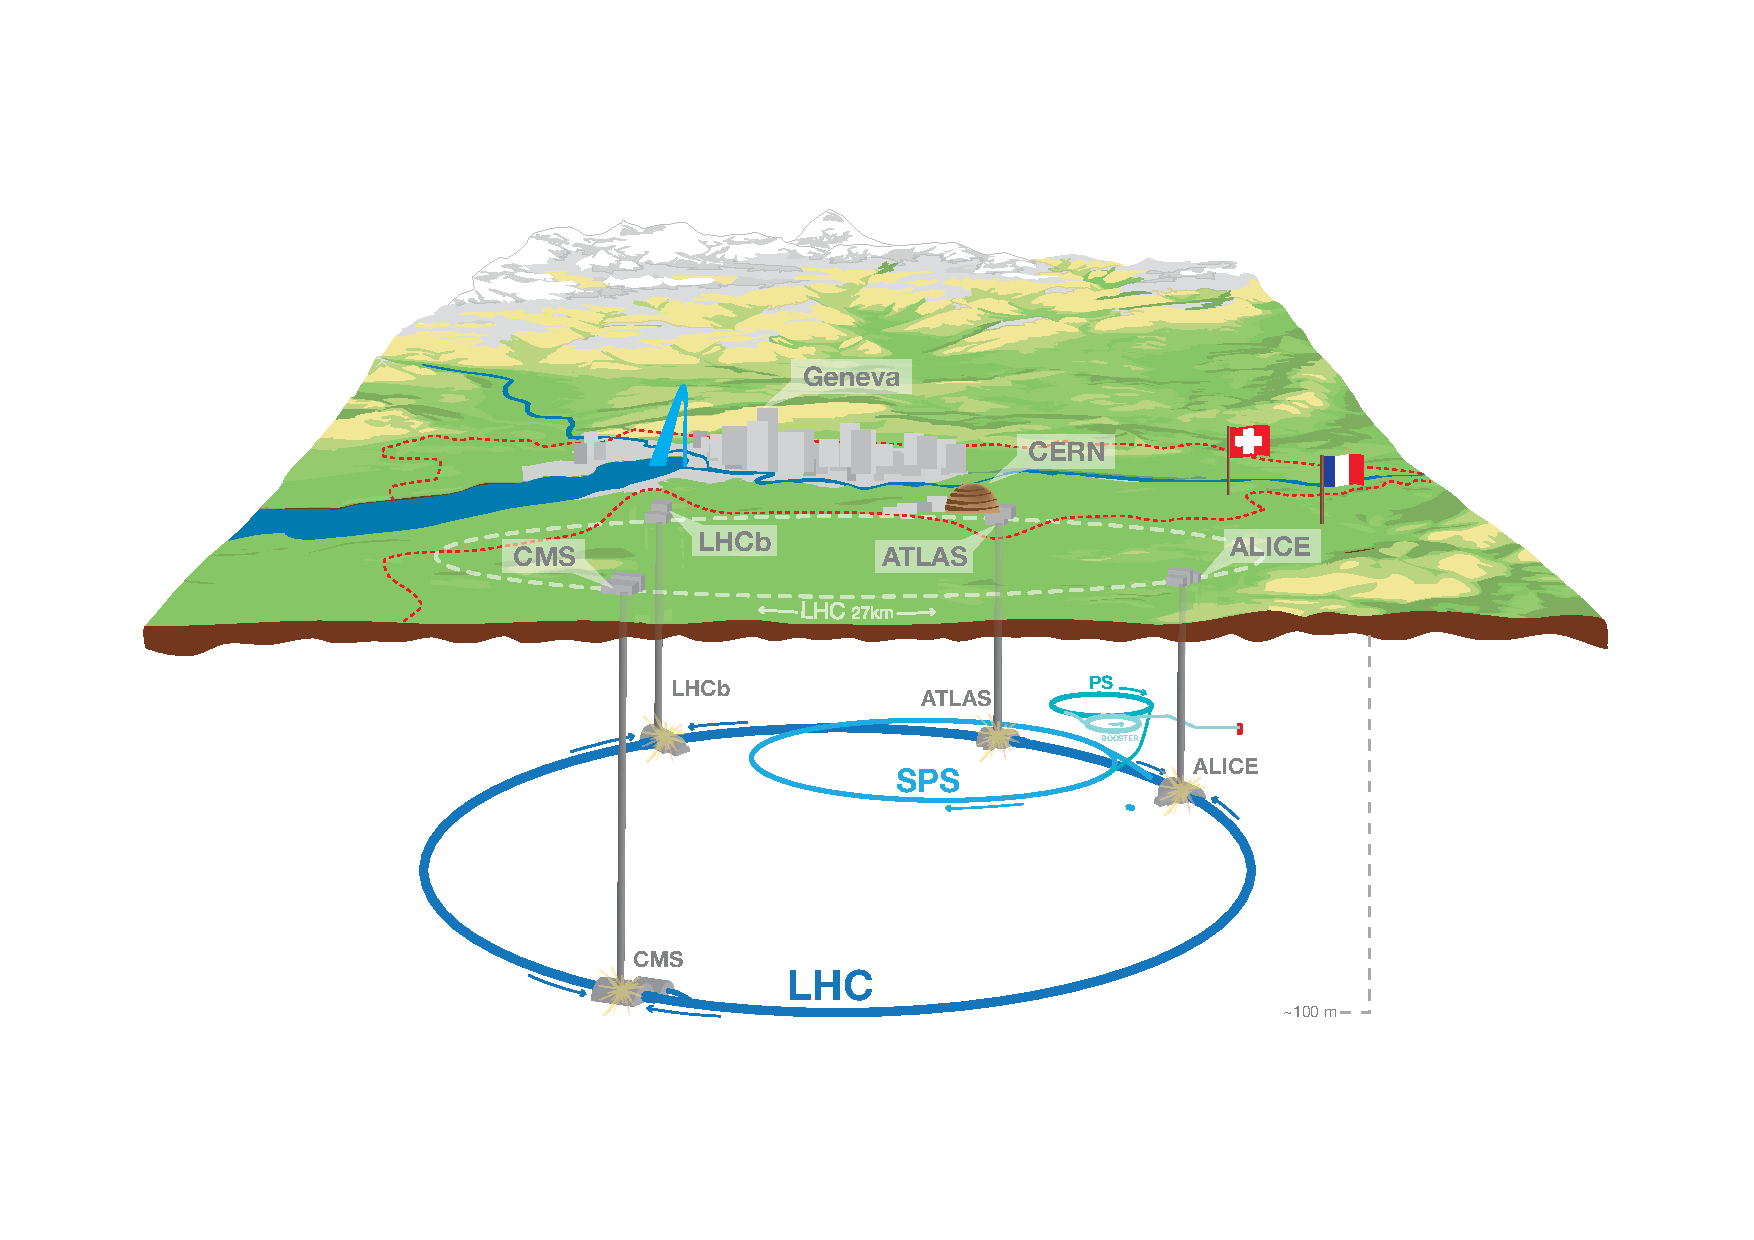
\includegraphics[width=16cm]{fig/Intro/LHCoverview.pdf}
\caption[LHC 加速器の概観]{LHC 加速器の概観\cite{cern_general_photo}}
\label{LHCoverview}
\end{figure}

ATLAS(A Toroidal LHC Apparatus)検出器は複数の検出器で構成された大型汎用検出器である。図\ref{ATLASdetector}に全体像を示す。ATLAS検出器は主に内部飛跡検出器、カロリメーター、ミューオンスペクトロメーターという3つの検出器群から成り立っている。最内層に設置された内部飛跡検出器はソレノイド磁石を使用して、荷電粒子の飛跡を再構成し、運動量を測定する。その外側に配置された電磁カロリメーターとハドロンカロリメーターでは、それぞれ電子、光子およびハドロンのエネルギーを測定する。最外層にあるミューオンスペクトロメーターでは内側の検出器を透過してきたミューオンを捉え、トロイダル磁石を使用してその運動量を測定する。本研究のテーマであるミューオンスペクトロメーターについては\ref{}節で詳しく説明する。

\begin{figure} 
    \centering
    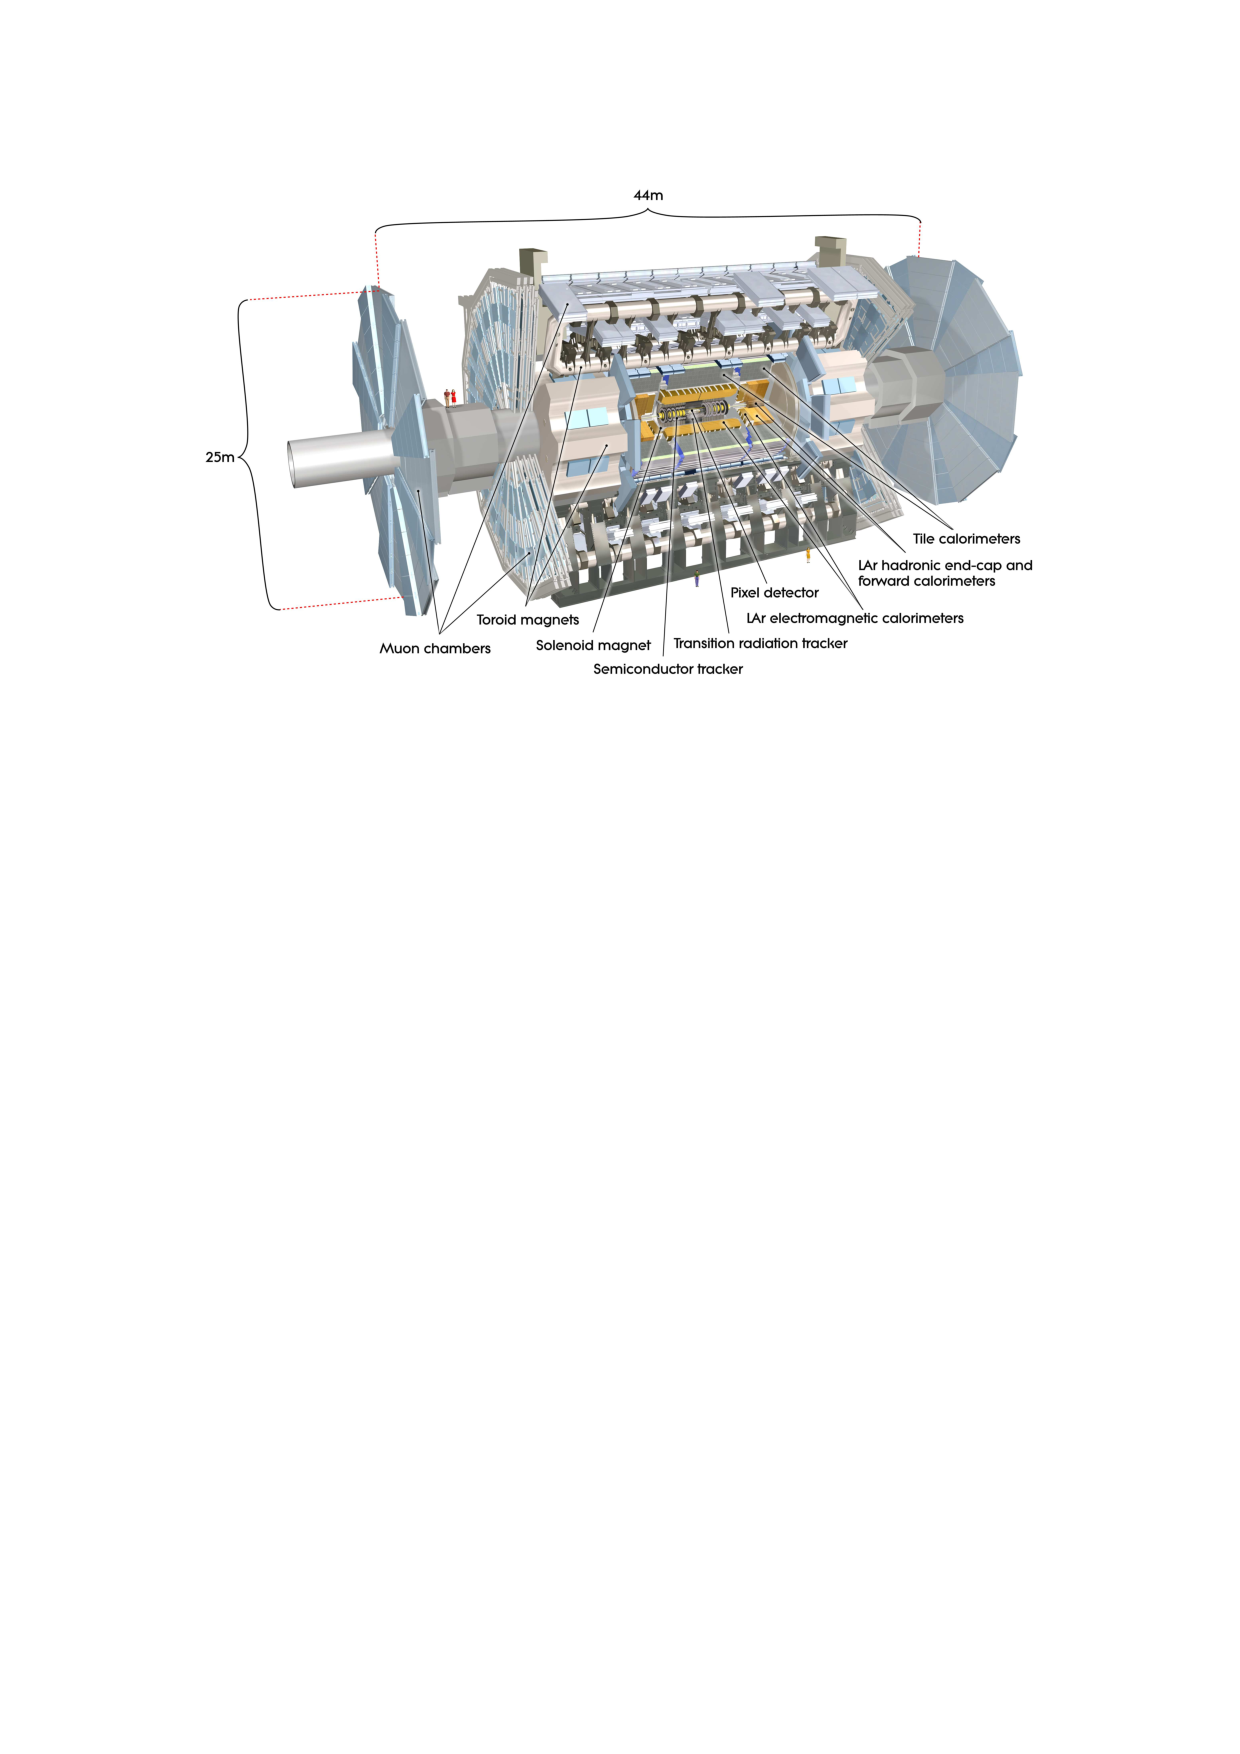
\includegraphics[width=16cm]{fig/Intro/ATLASdetector.pdf}
    \caption[ATLAS検出器の概要]{ATLAS検出器の概要図\cite{JINST:2008}}
    \label{ATLASdetector}
\end{figure}

LHC-ATLAS実験では陽子陽子衝突が40 MHzで行われ、1回のバンチ衝突ごとに約10\,Mb程度の信号が生じる。これは1秒間に約1\,Pbpsのデータ量に相当し、これらの全てのデータをストレージに転送し、保存することは技術的に不可能である。一方、陽子陽子衝突で生じるほとんどの事象は非弾性散乱など物理解析にとって興味の薄いものである。実際にATLAS実験で測定された各物理過程の反応断面積を図\ref{LHCcrosssection}に示す。pp→Xで示された陽子衝突の断面積に比べて、pp→Hで示されるヒッグス生成事象の断面積はO($10^10$)倍小さい。このような莫大な背景事象の中から、興味のある事象のみを選別し保存するシステムをトリガーシステムと呼ぶ。
新粒子探索や標準模型の精密測定の多くの解析において、統計量はその解析感度を決定する重要な要素である。ATLAS実験において、より洗練されたトリガーシステムを構築し、興味のある物理事象への感度を高めていくことは、物理探索に直結する重要な課題である。\par

\begin{figure} 
    \centering
    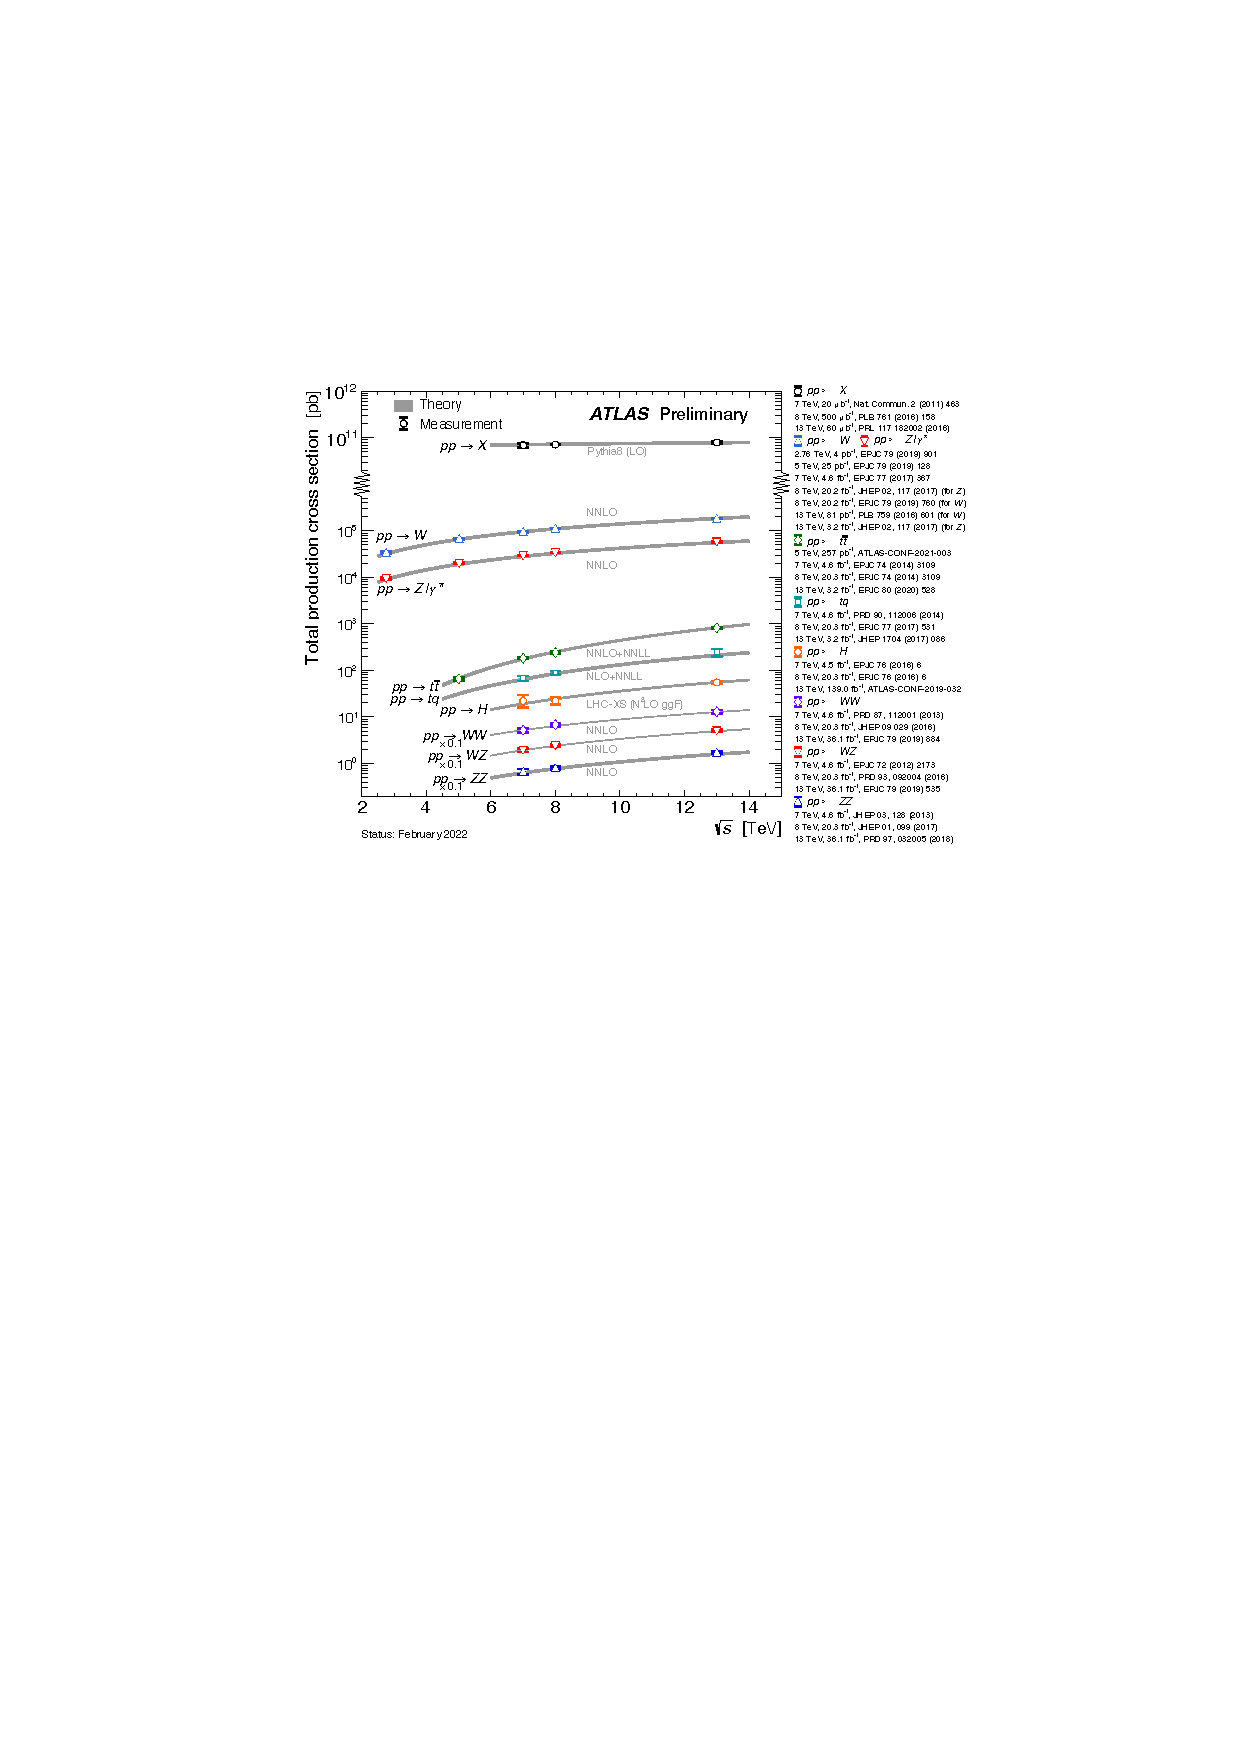
\includegraphics[width=16cm]{fig/Intro/LHCcrosssection.pdf}
    \caption[陽子陽子衝突における各反応事象の断面積]{陽子陽子衝突における各反応事象の断面積 \cite{atlas_phys_pub_hllhc}}
    \label{LHCcrosssection}
\end{figure}


\section{高輝度LHC実験に向けたPhase-\two アップグレード}
\label{sec_intro_phase2upgrade}

\begin{figure} 
\centering
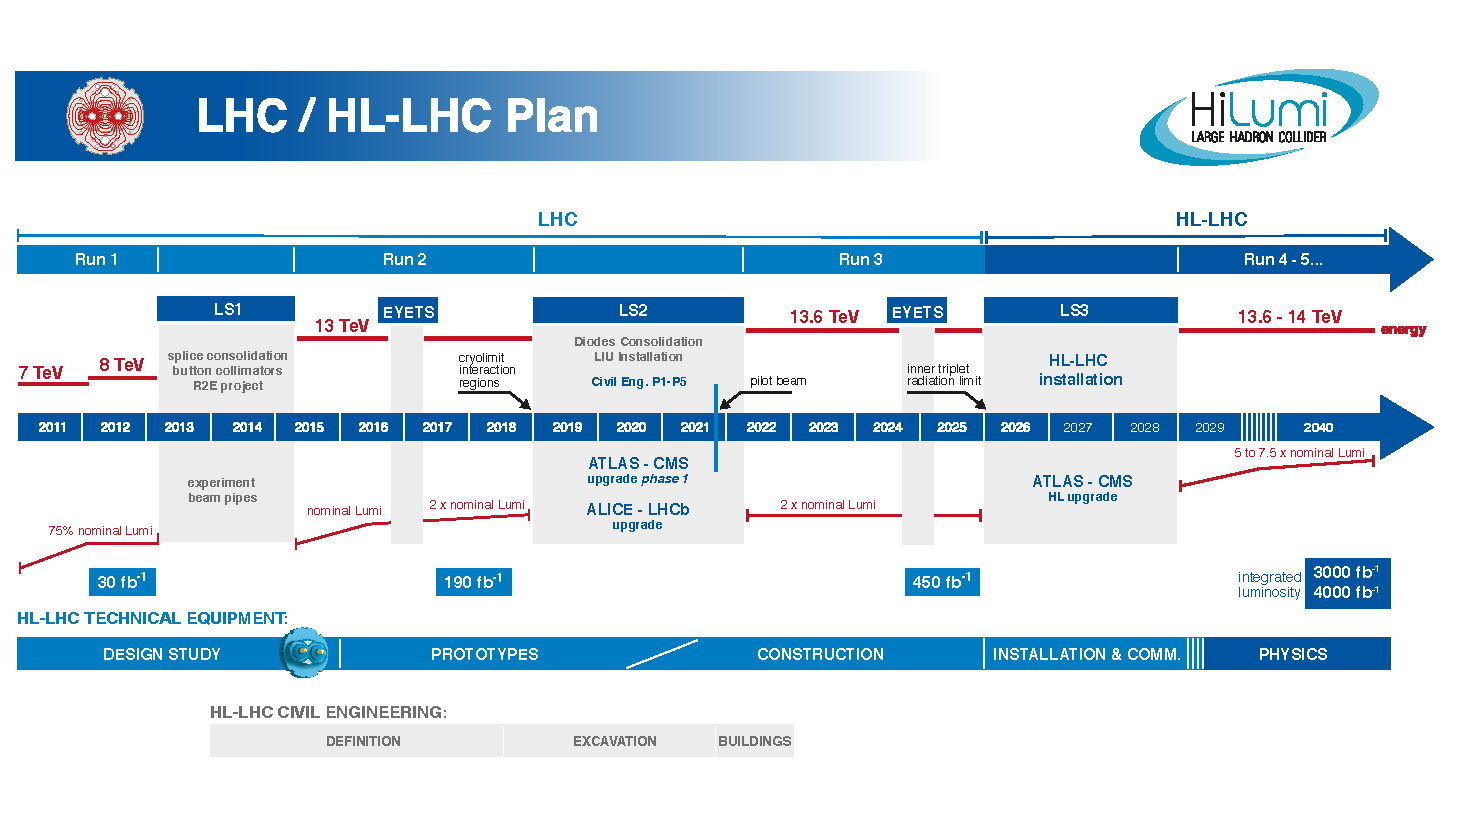
\includegraphics[width=16cm]{fig/Intro/LHCschedule.pdf}
\caption[LHC実験のスケージュール]{LHC実験のスケジュール\cite{cern_hllhc_industry}}
\label{LHCschedule}
\end{figure}

LHC実験は2010年から本格的に稼働を開始し、2024年現在、第三期運転(Run3)が進行中である。Run3では2025年までに累計450\,$\mathrm{fb}^{-1}$の統計量が蓄積することが予定されている。その後、3年間のLong Shutdown(LS3)を経てLHC実験は高輝度LHC実験に大幅にアプグレードされる。高輝度LHC実験では瞬間最高ルミノシティが現在のの$2\times10^{34}\,\mathrm{cm}^{-2}\mathrm{s}^{-1}$から$5 \text{~} 7.5\times10^{34}\,\mathrm{cm}^{-2}\mathrm{s}^{-1}$に増強され、2040年の実験終了までに3000 ~ 4000\,$\mathrm{fb}^{-1}$の統計量が貯められる予定である。一方で、高輝度LHC実験では瞬間ルミノシティの増加に伴い、一回のバンチ衝突ごとに発生する陽子陽子衝突数(パイルアップ)が増加し、背景事象が大幅に増加する。高輝度環境下で背景事象を適切に削減し、興味のある事象だけを効率的に取得するためには検出器やトリガーシステムのアップグレードが不可欠である。\par

図\ref{Ptthreshold}に高輝度LHC実験で現行のトリガーシステム(特に電子やミューオンの横方向運動量をもとに閾値を設定するシングルレプトントリガーシステム)を利用した場合の各物理事象へのアクセプタンスの見積を表す。現行のレプトンの運動量分解能や信号転送レートを維持したまま、信号事象や背景事象が増加すると、閾値を超えるレプトンの数が読み出し能力を超えるため、レプトンの横方向運動量閾値を50 GeV程度まで上げなくてはならない。対して、トリガーシステムをアップグレードしてシングルレプトンの運動量分解能を向上や、読み出し能力の増強を実現することができれば横方向運動量閾値を20 GeVまで低く抑えることができる。これにより、例えば、終状態に低運動量レプトンが生成される縮退したSUSY粒子の崩壊事象へのアクセプタンスは約4倍に増幅されることが見込まれる。


\begin{figure} 
\centering
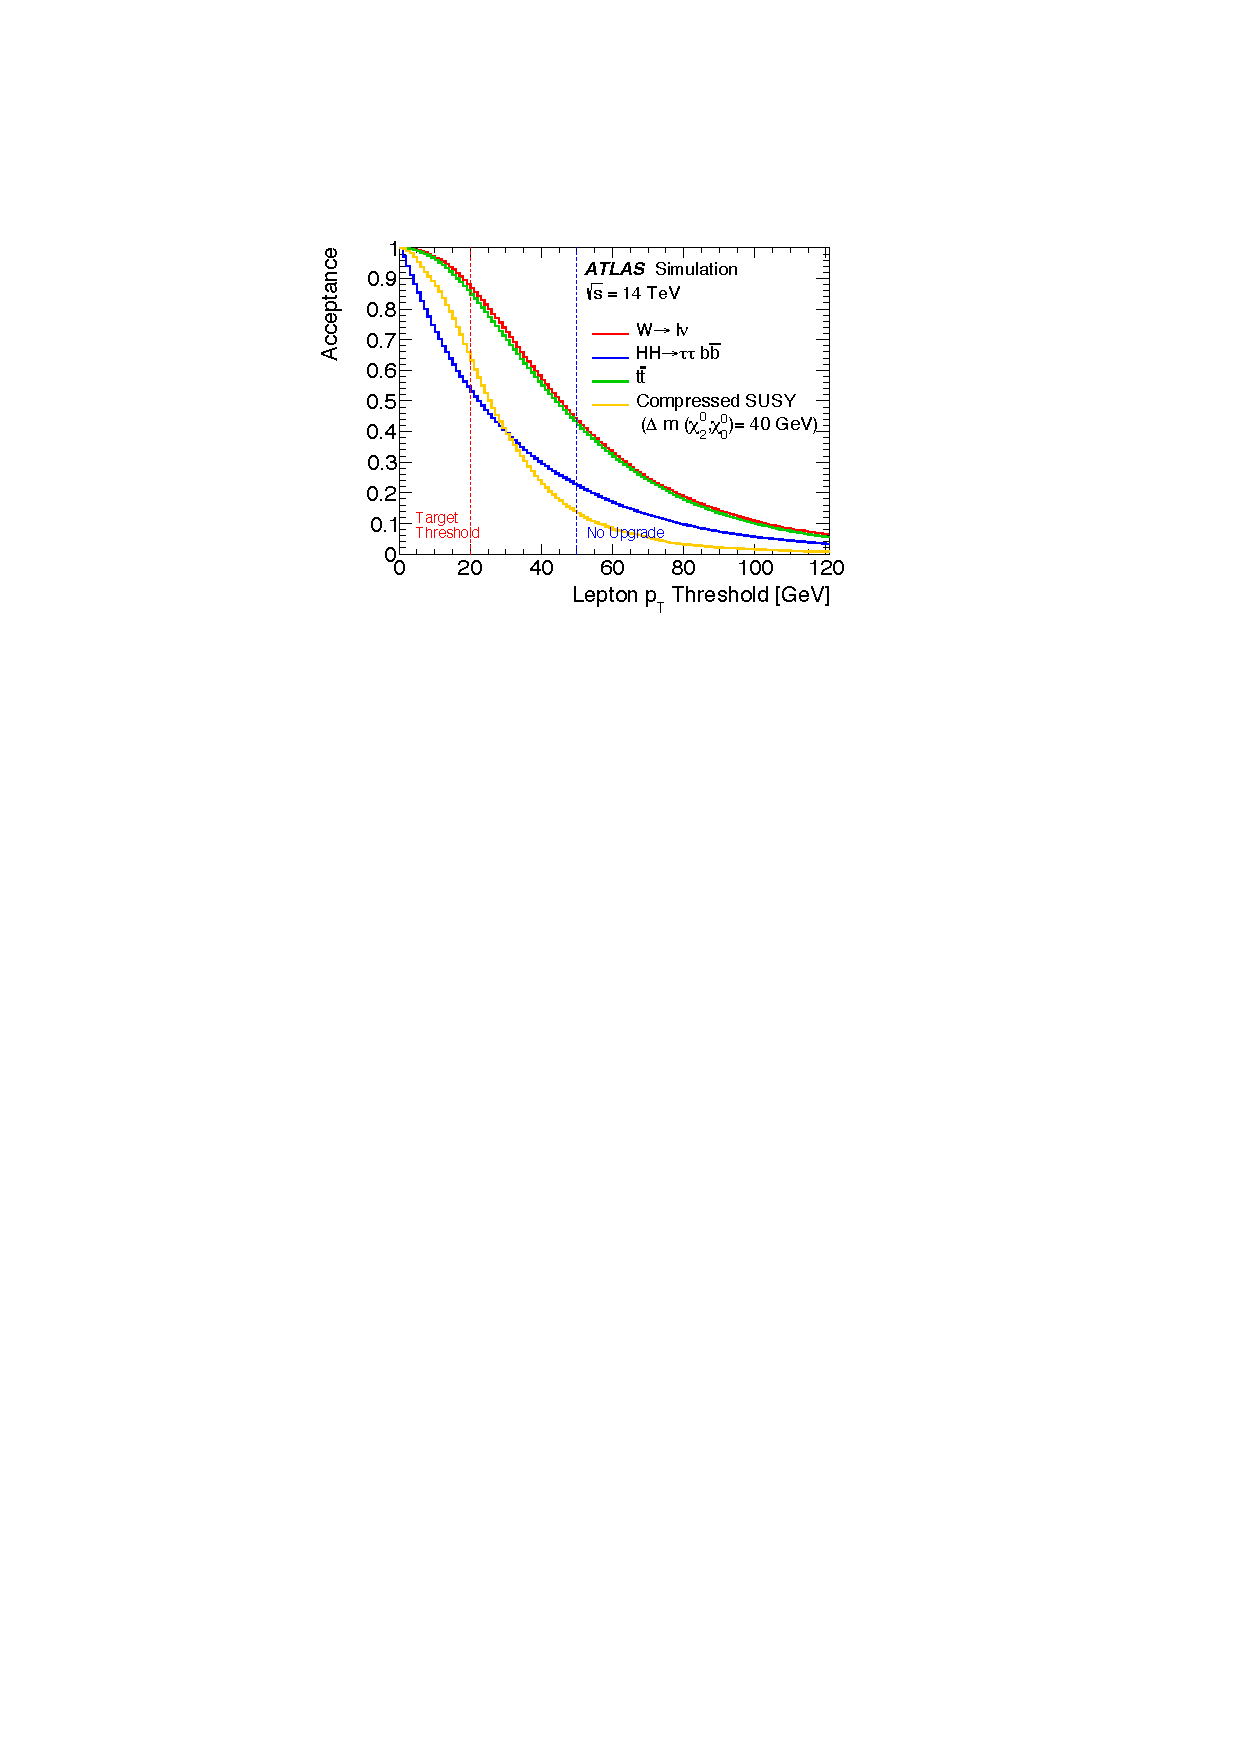
\includegraphics[width=16cm]{fig/Intro/Ptthreshold.pdf}
\caption[高輝度LHC-ATLAS実験の主なターゲットとなる事象における、レプトンの pT 閾値とアクセプタンスの関係]{高輝度LHC-ATLAS実験の主なターゲットとなる事象における、レプトンの pT 閾値とアクセプタンスの関係\cite{tdr_phase2tdaq_2017020}}
\label{Ptthreshold}
\end{figure}

\section{本論文の目的・内容と構成}
\label{sec_intro_purpose}






% \chapter{高輝度LHC-ATLAS実験に向けたTGC検出器システムのアップグレード}
\label{chap_TGC}

% この章では、自分の研究に関連する分野の歴史や現状について説明したり、研究を展開する上で重要となる知識の解説を行います。ここで使用している見出し「ガンマ線天文学…」はあくまで例ですが、もしCherekov Telescope Array(CTA)計画\footnote{省略語は必ず正式名称を先に書き、省略系は丸括弧に入れます。省略語はあくまで「以降このように略す」という用途だからです。また、日本語文章中で使う丸括弧は ()ではなく()です。}に携わる院生の書く修士論文であれば、ガンマ線天文学や宇宙線物理学全般について、現行望遠鏡とガンマ線観測の原理について、またCTA計画についての記述がこの章では期待されます。

% 場合によっては「序論」と合体させても良いですが、本章は比較的長くなり結論に直結しない情報もたくさん出てくるため、独立した章である方が読者は読みやすいでしょう。

% またこの章が長くなるときには、例えば「ガンマ線天文学」と「CTA計画」のように、2つの章に分割するというのも良いと思います。\footnote{注意書きの練習です。}

\section{LHC-ATLAS実験におけるTGC検出器}
本節では本研究のテーマである、Thin Gap Chamber ( TGC ) 検出器について説明する。それに先んじて、ATLAS検出器で使われる座標系と、ATLAS検出器における磁場構造について説明する。

\subsection{ATLAS実験における座標系}
\label{subsec_ATLAScordination}
ATLAS実験では主に2種類の座標系が用いられる。図\ref{ATLAScordination}にその概要を示す。1つ目の座標系である直交座標系は、原点を検出器中心に取りLHCの中心方向を$x$、地上方向を$y$に取った右手系で定義する。この時、$z$軸はビーム軸方向に沿って定義される。$z>0$ の領域をA side、$z<0$の領域をC sideと呼ぶ。2つ目の座標系である円筒座標系は、ビーム軸を中心とした方位角方向を$\phi$、ビーム軸からの天頂角方向を$\theta$、同型方向を$R$と定義する。また、$\theta$ 方向を表す変数として、擬ラピデティ  (Pseudorapidity)
\begin{equation}
    \eta = -\ln(\mathrm{tan}\frac{\theta}{2})
\end{equation}
を定義し、粒子の四元運動量を記述する際\footnote{$\eta$はハドロンコライダーで生じる物理現象を説明する際によく利用される。2粒子間の$\eta$の差は$z$軸方向のブーストに対してローレンツ不変であり、始状態の粒子の$z$方向の運動量に関わらず崩壊事象を統一的に記述することができる。}やビーム衝突点から見た時の各検出器の立体角を議論する際に利用する。本研究で扱うミューオンシステムの議論でも$\eta$を利用し、|$\eta$| < 1.05の円筒側面領域をバレル領域 ( Barrel ) 、|$\eta$| > 1.05の円筒底面領域をエンドキャップ ( Endcap ) と区別する。

またATLAS実験では粒子の状態を表す物理量として$z$軸垂直方向の運動量 (横方向運動量、\pt) やエネルギー (横方向エネルギー、$E_{\mathrm{T}}$) を利用する。
高エネルギーの陽子陽子衝突は、陽子の内部構造であるパートン同士の衝突であり、その担う運動量の差により衝突重心系は実験室系では$z$軸方向にローレンツブーストされている。一方で横方向の運動量は (交差角の効果や、フェルミ運動量を除けば) 実験室系で厳密にゼロとなる。終状態粒子の運動量の$z$軸方向の成分はパートン同士の運動量の非対称による寄与が大きく、パートン同士の衝突重心系の全エネルギーの良い指標にはならない。一方で横方向の運動量はパートン同士の衝突重心系の全エネルギーの良い指標となるため、横方向運動量や横方向エネルギーが事象選別の重要な指標となる。同様にオンライン事象選別であるトリガーでも横方向運動量、横方向エネルギーを指標にして興味のある事象を選択する。

\begin{figure} 
\centering
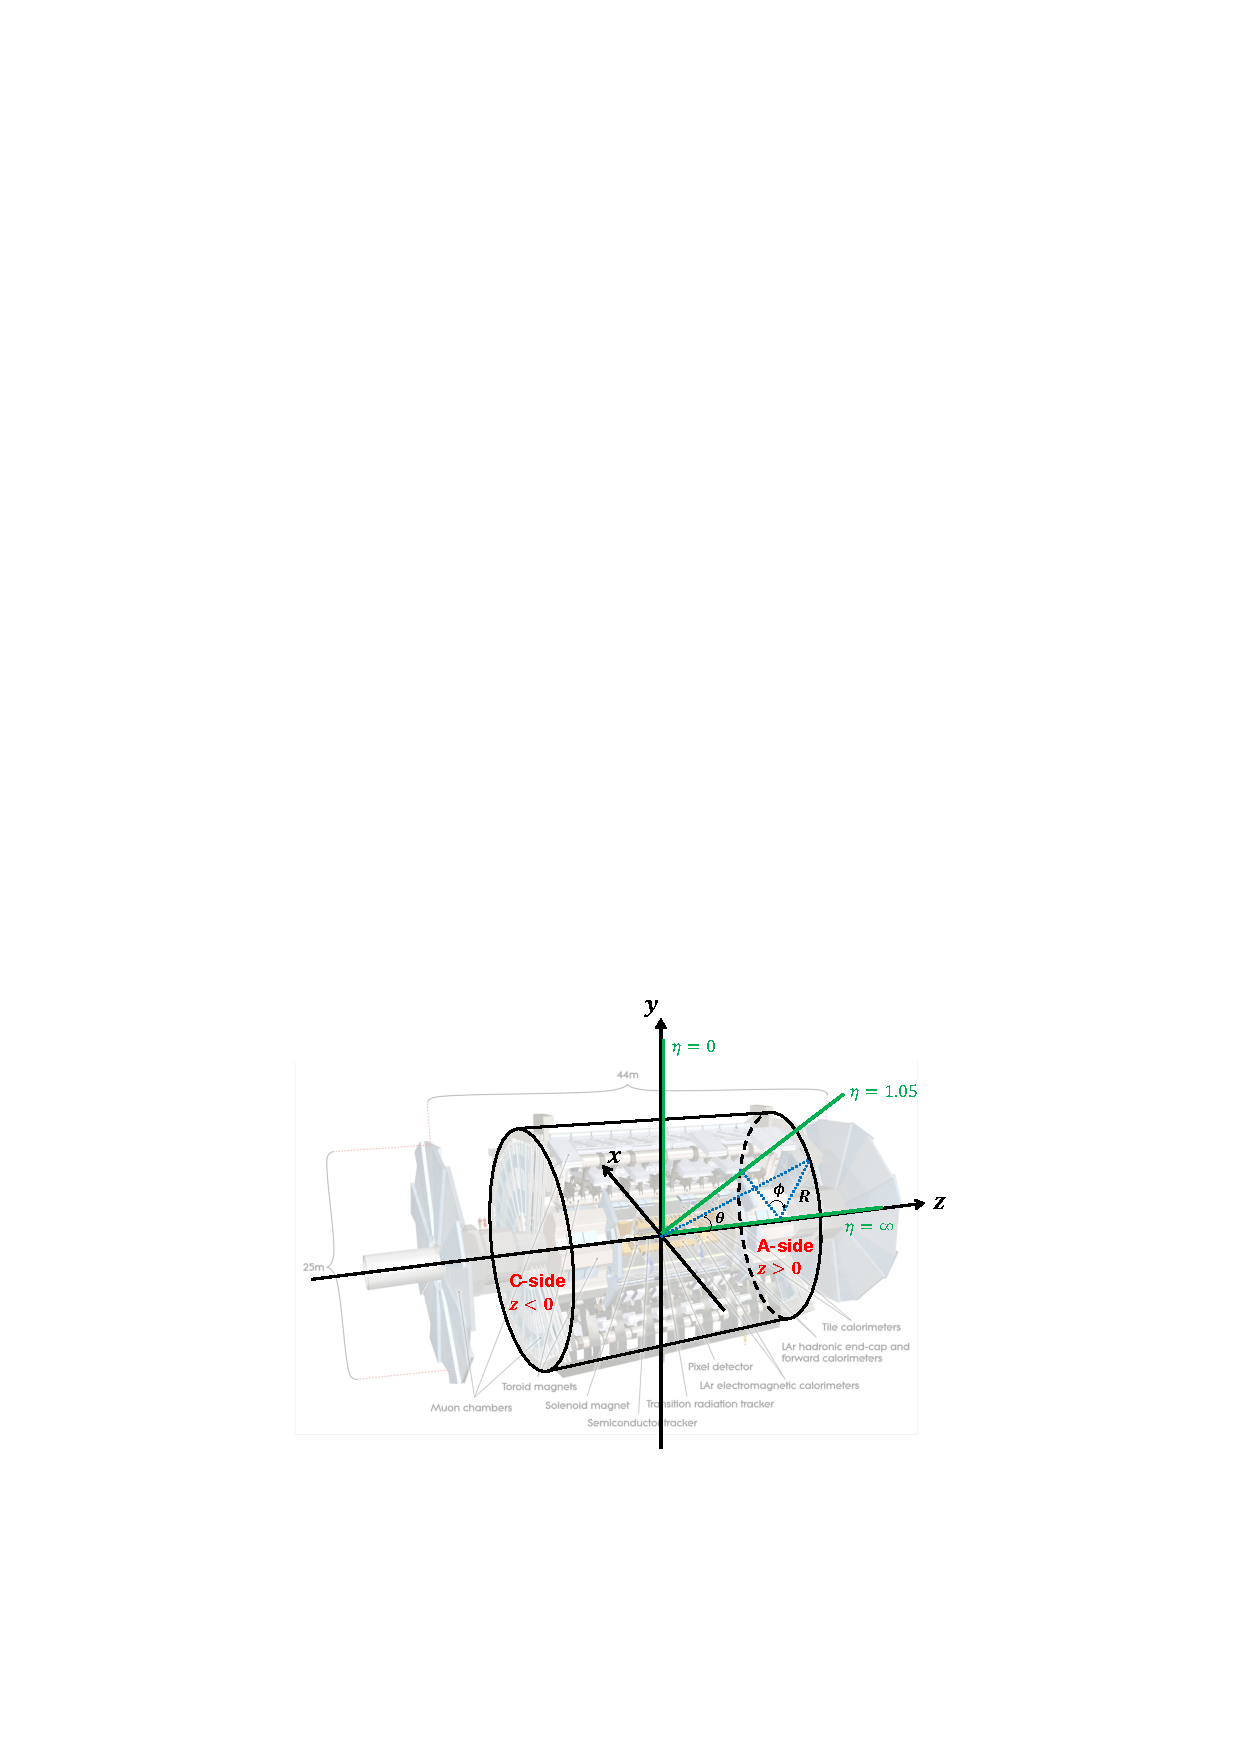
\includegraphics[width=16cm]{fig/Intro/ATLAScordination.pdf}
\caption[ATLAS検出器における座標系]{ATLAS検出器で用いられる座標系。直交座標系はtビーム軸方向を$z$軸、LHC中心方向を$x$軸正の向きとした右手系で定義される。$z>0$をA side、$z<0$をC sideと呼ぶ。円筒座標系も利用され、特にビーム衝突点から見た時の各検出器の立体角を議論する際などに利用する。最外層のミューオンシステムは|$\eta$| = 1.05でバレル領域とエンドキャップ領域に分かれる。}
\label{ATLAScordination}
\end{figure}

\subsection{ATLAS検出器における超伝導磁石}
\label{subsec_magnet}
ATLAS検出器では荷電粒子の運動量を測定するため、2種類の超伝導磁石が設置されている。図\ref{ATLASmagnet}にATLAS検出器における超伝導磁石の配置を示す。1つ目は、内部飛跡検出器内で荷電粒子を曲げるのに利用されるソレノイド磁石である。ソレノイド磁石は内部飛跡検出器とカロリメーターの間の領域に設置され、$z$軸方向の磁場を生成する。2つ目は、内部検出器を透過してきたミューオンを曲げるのに利用されるトロイド磁石である。トロイド磁石はバレル部用とエンドキャップ部用で2種類用意される。バレル部とエンドキャップ部のトロイド磁石はそれぞれ$\phi$方向に8回対称の構造をとっており、互いの干渉を避けるため22.5度ずらして設置される。トロイド磁石は主に$\phi$方向の磁場を生成し、$\eta$方向に荷電粒子を曲げるが、磁石の構造によって磁場は場所ごとに不均一になっている。

\begin{figure} 
    \centering
    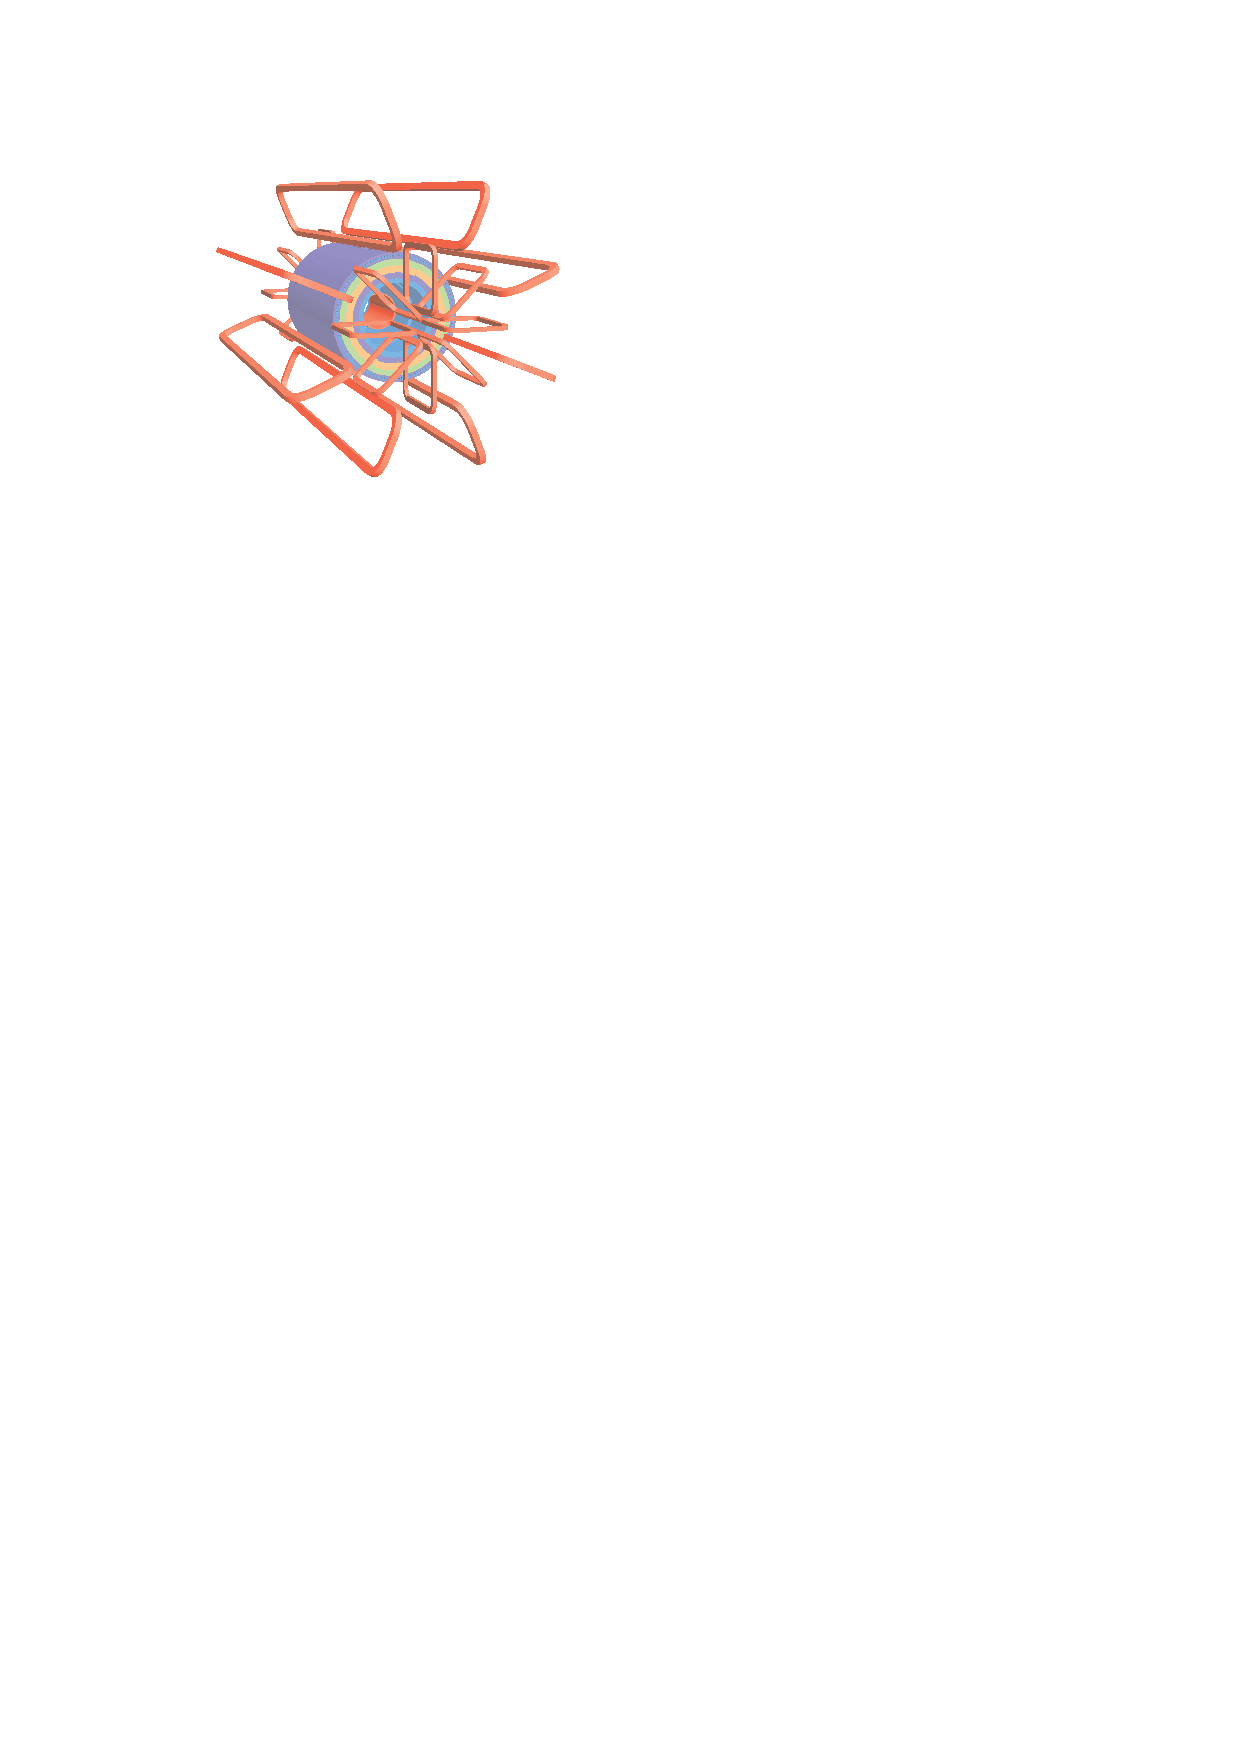
\includegraphics[width=12cm]{fig/Intro/ATLASmagnet.pdf}
    \caption[超伝導磁石の配置]{超伝導磁石の配置\cite{JINST:2008}。内部飛跡検出器を囲うようにソレノイド磁石が、カロリメーターの外側にトロイド磁石が設置されている。トロイド磁石はバレル用のものとエンドキャップ用のものが22.5度ずらして設置される。}
    \label{ATLASmagnet}
\end{figure}

\subsection{ミューオンスペクトロメーター}
\label{subsec_Muonspectrometer}
ミューオンスペクトロメーターはATLAS検出器最外層に設置された検出器で、カロリーメーターを透過したミューオンの横方向運動量を測定する役割を担う。
ミューオンスペクトロメーターはトロイド磁場の構造に合わせて$\phi$方向に8回対称になっており、そのうちバレル部のトロイド磁石が位置する領域を Small sector、トロイド磁石間に位置する領域をLarge sectorと呼ぶ。ミューオンスペクトロメーターの全体像を図\ref{Muonspectrometer2}に示す。

高輝度LHC-ATLAS実験においてエンドキャップ部ミューオントリガーに関わる検出器としては、TGC検出器、New Small Wheel (NSW)、Resistive Plate Chamber (RPC)、Monitored Drift Tube (MDT) 、Tile カロリメーターがある。TGC検出器については後ほど詳述する。NSWはエンドキャップトロイド磁場の内側に設置されたトリガーおよび精密測定用のミューオン検出器であり、1.3 < |$\eta$| < 2.7の全$\phi$方向をカバーする。small-strip TGC (sTGC) とMicromegas (MM) の2種類の検出器を4層ずつ組み合わせた構造をしており、荷電粒子が通過した位置および飛跡の角度情報を取得する。RPCは |$\eta$| < 1.05のバレル領域に設置されたトリガー用のミューオン検出器である。直交するストリップで$\eta$と$\phi$の位置情報を読み出す。Run 3以降ではSmall sector にRPC BIS78 というエンドキャップ領域に位置する検出器が設置され、エンドキャップミューオントリガーにおいても利用される。MDTはバレル領域およびエンドキャップ領域に設置された精密測定用のミューオン検出器である。ドリフトチューブを6層または8層並べた構造をとっており、荷電粒子が通過した位置および飛跡の角度情報を再構成する。MDTはドリフト時間が長く、Run 3までは初段トリガーで用いることができなかったが、高輝度LHC-ATLAS実験からは拡張されるレイテンシーを活用して、初段トリガーにも用いられる。Tile カロリメーターは電磁カロリメーターの外側に設置されたハドロンカロリメーターであり、複数の層が重なった構造をとっている。最外層に到達する粒子のほとんどがミューオンであることを利用して、エンドキャップ領域のトリガー判定に用いられる。


\begin{figure}
\begin{minipage}[b]{1.0\linewidth}
\centering
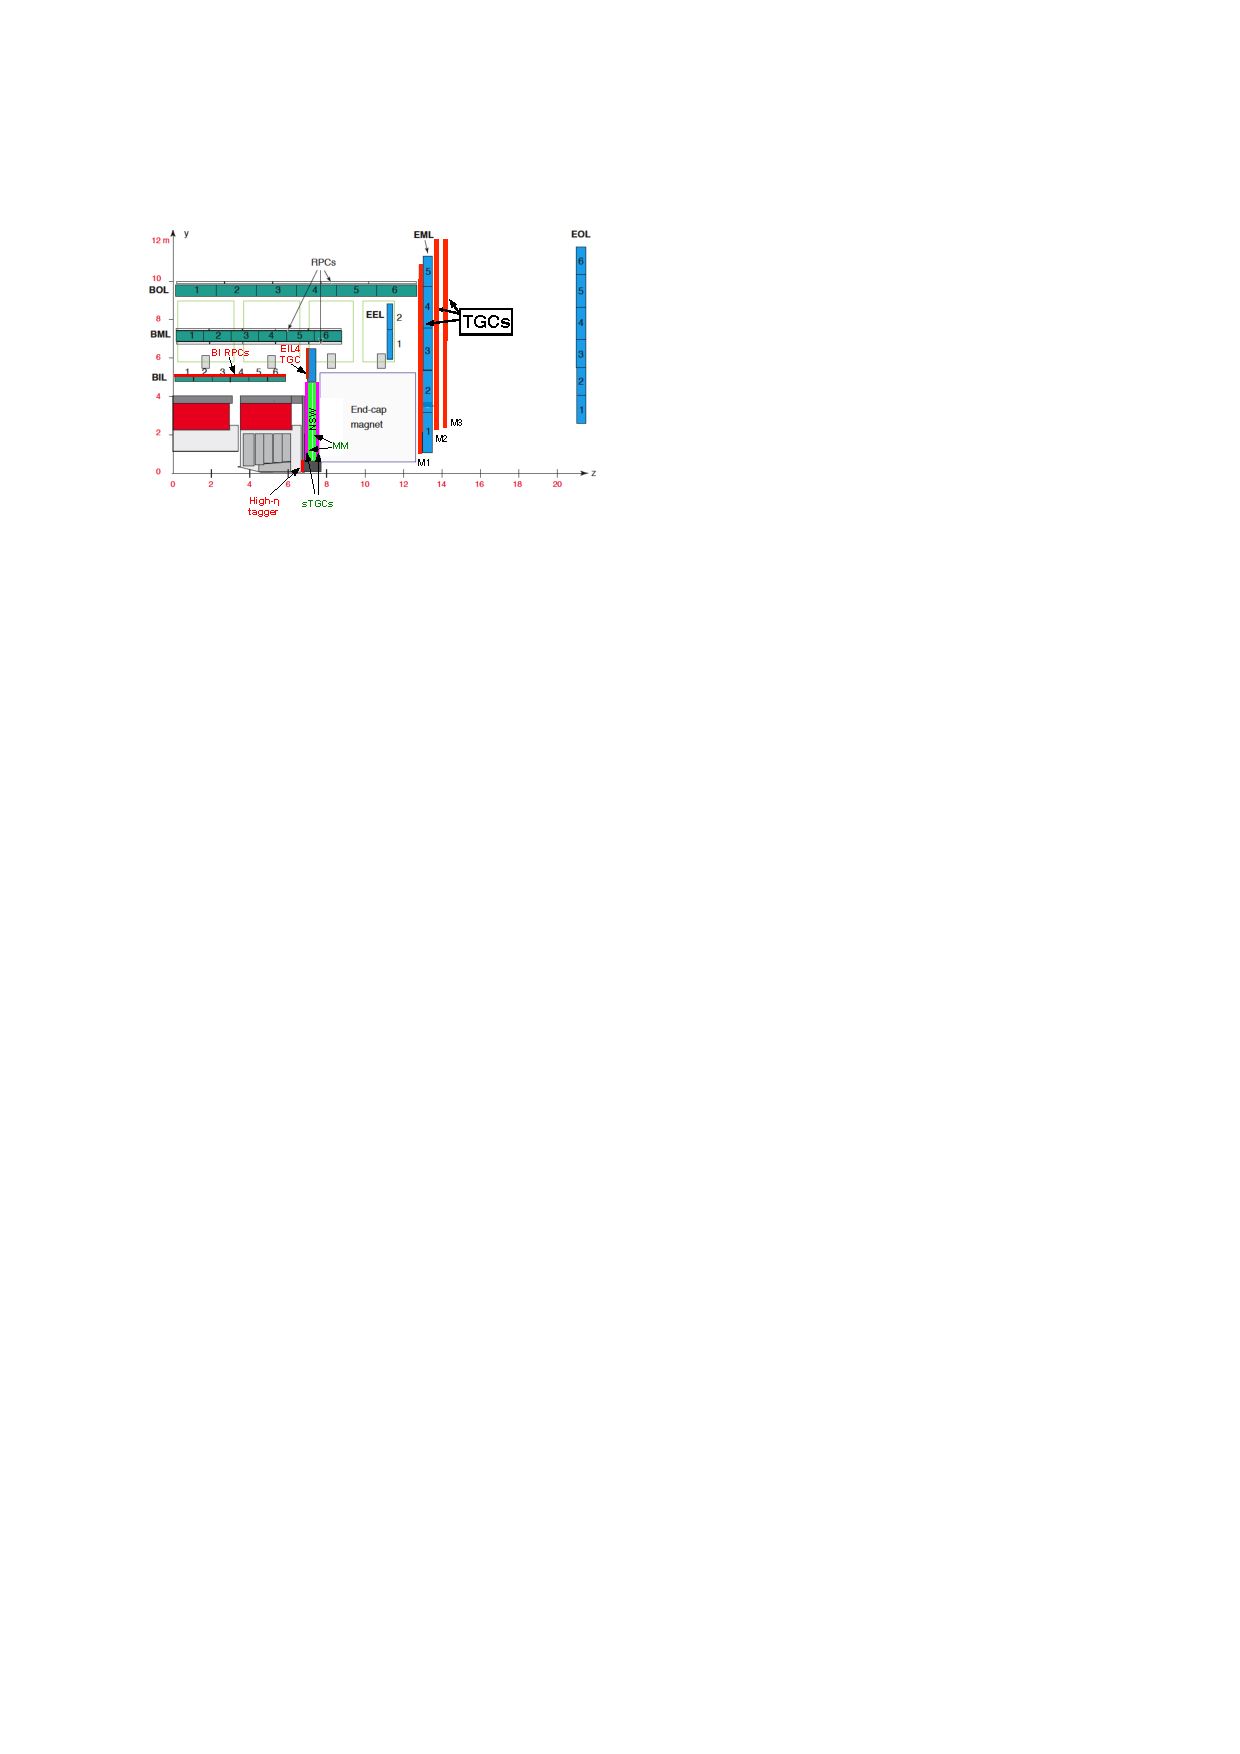
\includegraphics[width=16cm]{fig/Intro/MuonSpe_Large.pdf}
\subcaption{Large sectorでのミューオン検出器の配置}
\end{minipage}\\
\begin{minipage}[b]{1.0\linewidth}
\centering
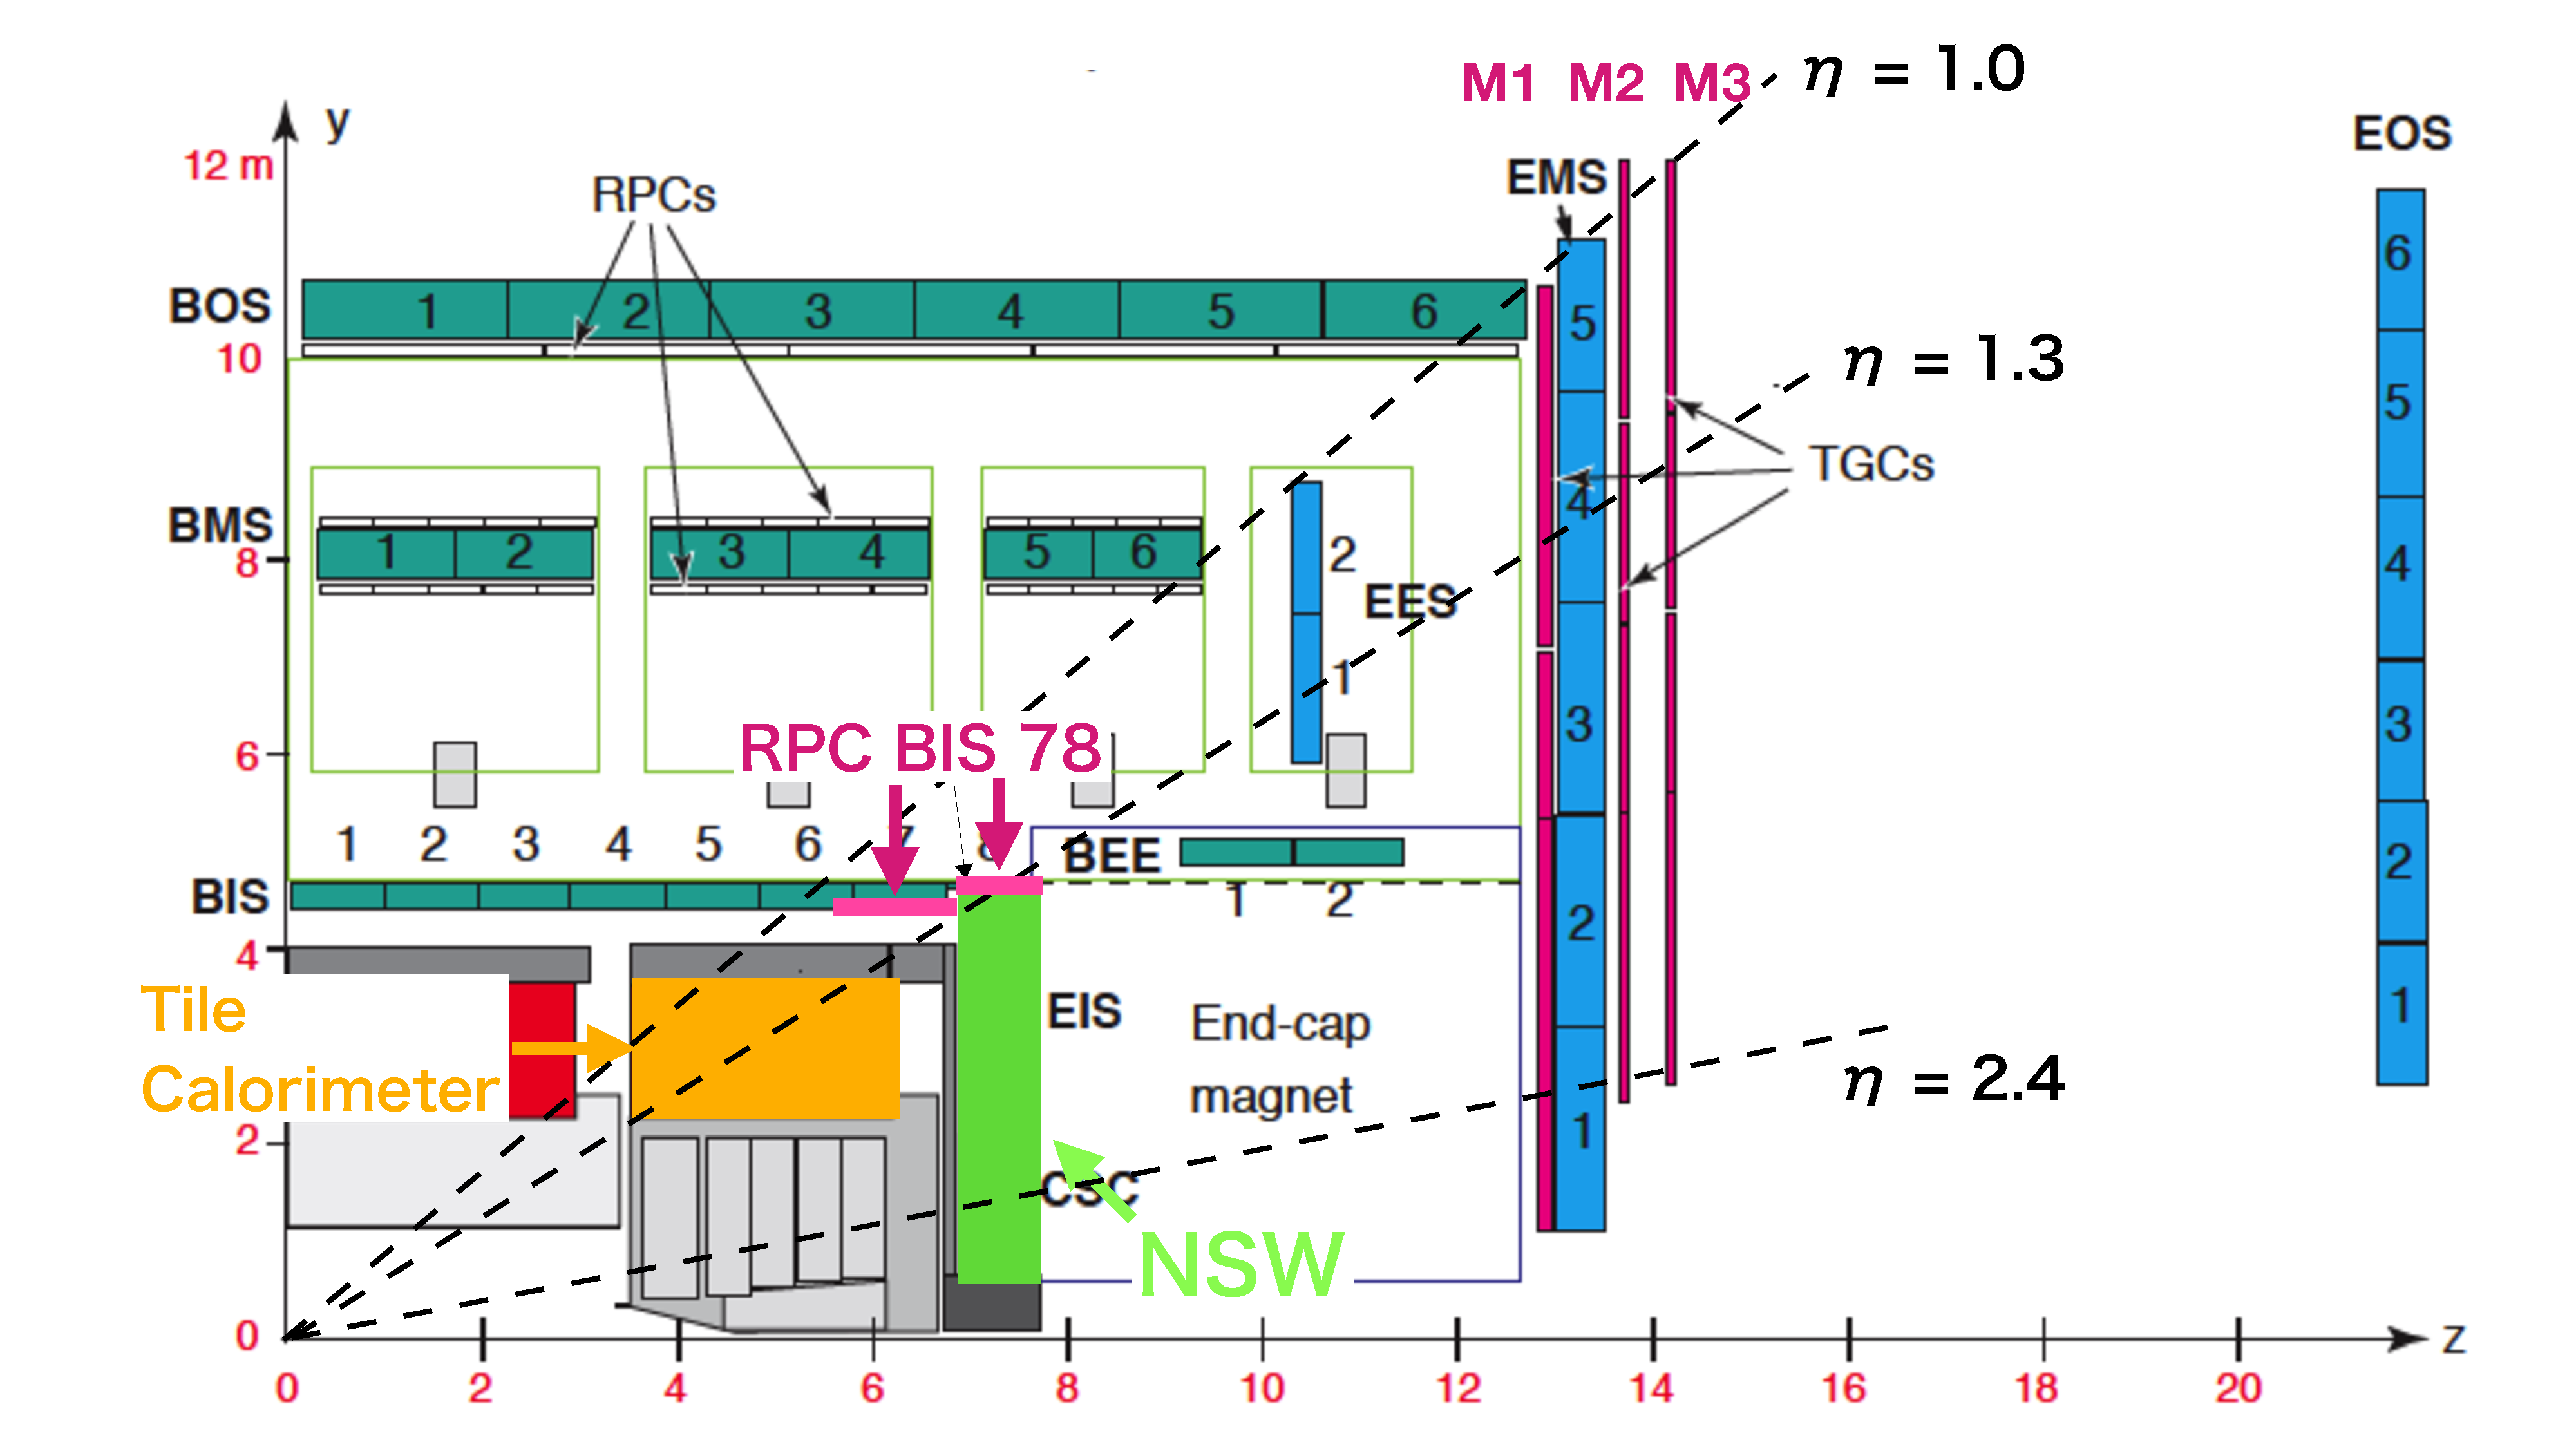
\includegraphics[width=16cm]{fig/Intro/MuonSpe_small.pdf}
\subcaption{Small sectorでのミューオン検出器の配置}
\end{minipage}%
\caption[高輝度LHC-ATLAS実験でのミューオンスペクトロメーターの$R$-$z$平面断面図]{高輝度LHC-ATLAS実験でのミューオンスペクトロメーターの$R$-$z$平面断面図\cite{tdr_phase2muon_2017017}。TGC BW 以外のミューオンスペクトロメーターはトロイドマグネットの磁場構造に合わせて8回対称になっており、$\phi$方向にLarge Sector、Small sectorという2種類のsectorに分かれている。エンドキャップ部のミューオントリガーには1.05 < |$\eta$| < 1.3の領域ではTGC、RPC BIS78、TGC EIL4、Tile カロリメーターが、1.3 < |$\eta$| < 2.4の領域ではTGCとNSWが用いられる。}
\label{Muonspectrometer2}
\end{figure}

\subsubsection*{TGC検出器}
TGC検出器は1.05 < |$\eta$| < 2.4のエンドキャップ領域に設置されたミューオントリガー用の検出器である。エンドキャップトロイド磁石より内側に位置するEndcap Innner  (EI) と外側に位置するBig Wheel  (BW) に大別される。TGC BWは$z$方向に3つのステーションが連なって構成され、衝突点に近い方からM1、M2、M3ステーションと呼ぶ (図\ref{Muonspectrometer2}参照)。各ステーションは2層または3層のガス層で構成されており、2層のものをdoublet、3層のものをtripletと呼ぶ。BWではM1がtriplet、M2、M3がdoubletになっている。

TGCチェンバーの構造を図\ref{TGC_structure}に示す。TGCはアノードワイヤー間隔が1.8 mm、アノードとGNDの間隔が1.4 mmであるMWPCである。ワイヤーは$R$方向、ストリップは$\phi$方向に直交して張られており、それぞれのヒット信号からミューオンが通過した2次元位置を検出することができる。ガス層には$\mathrm{CO_2}/n\text{-}\mathrm{C_5H_{12}}$が55:45で混合されたガスが充填されている。荷電粒子がTGCに入射すると、電磁相互作用によりガス分子が電離される。電離した電子はワイヤーに印加された2.8 kVの電圧によりワイヤー方向に集められ、ワイヤー付近に到達すると強い電場により電子雪崩を生じる。ワイヤーでは電子雪崩で生じた正イオンのドリフトが、ストリップではそれらの鏡像電荷が電流信号として検出される。

\begin{figure}
\begin{minipage}[b]{.4\linewidth}
\centering
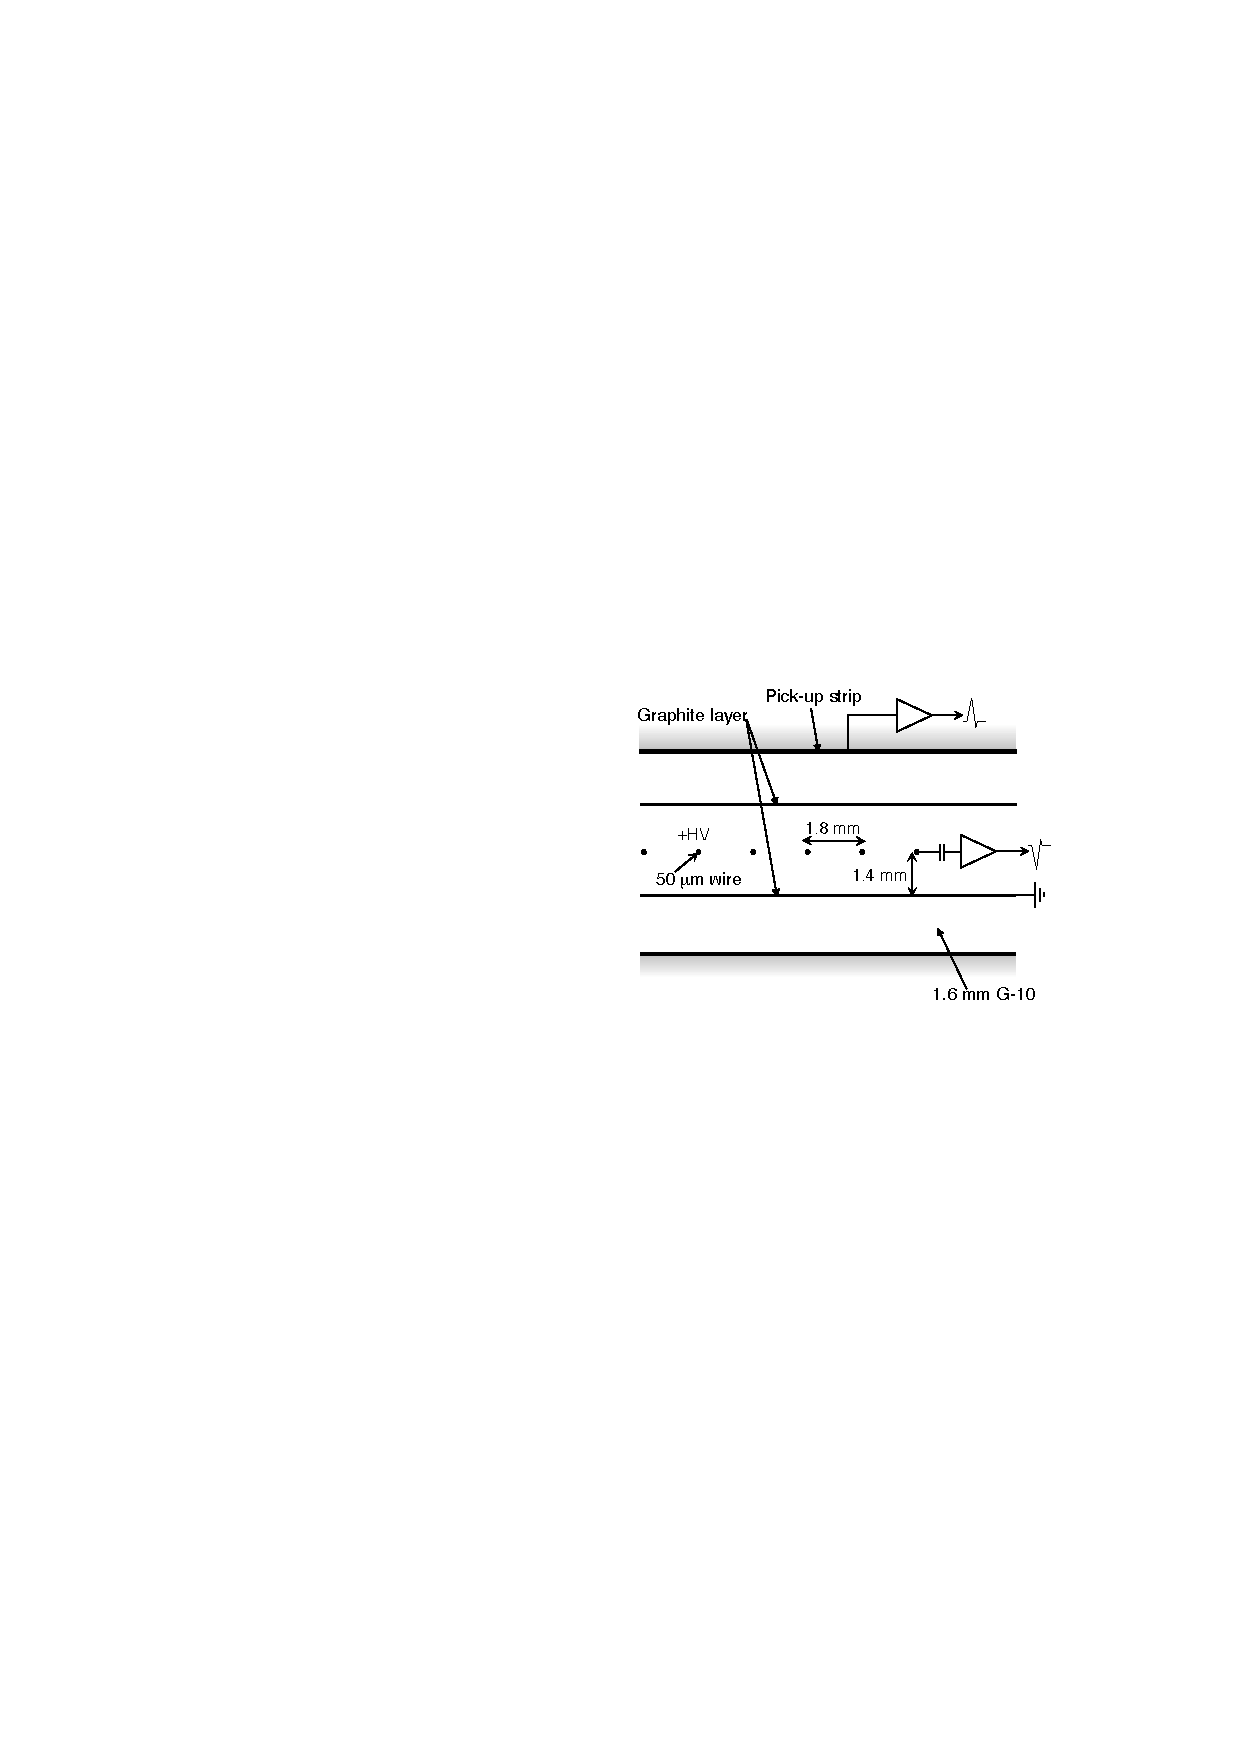
\includegraphics[height=5cm]{fig/Intro/TGC_structure.pdf}
\subcaption{TGCチェンバーの断面図}
\end{minipage}%
\begin{minipage}[b]{.6\linewidth}
\centering
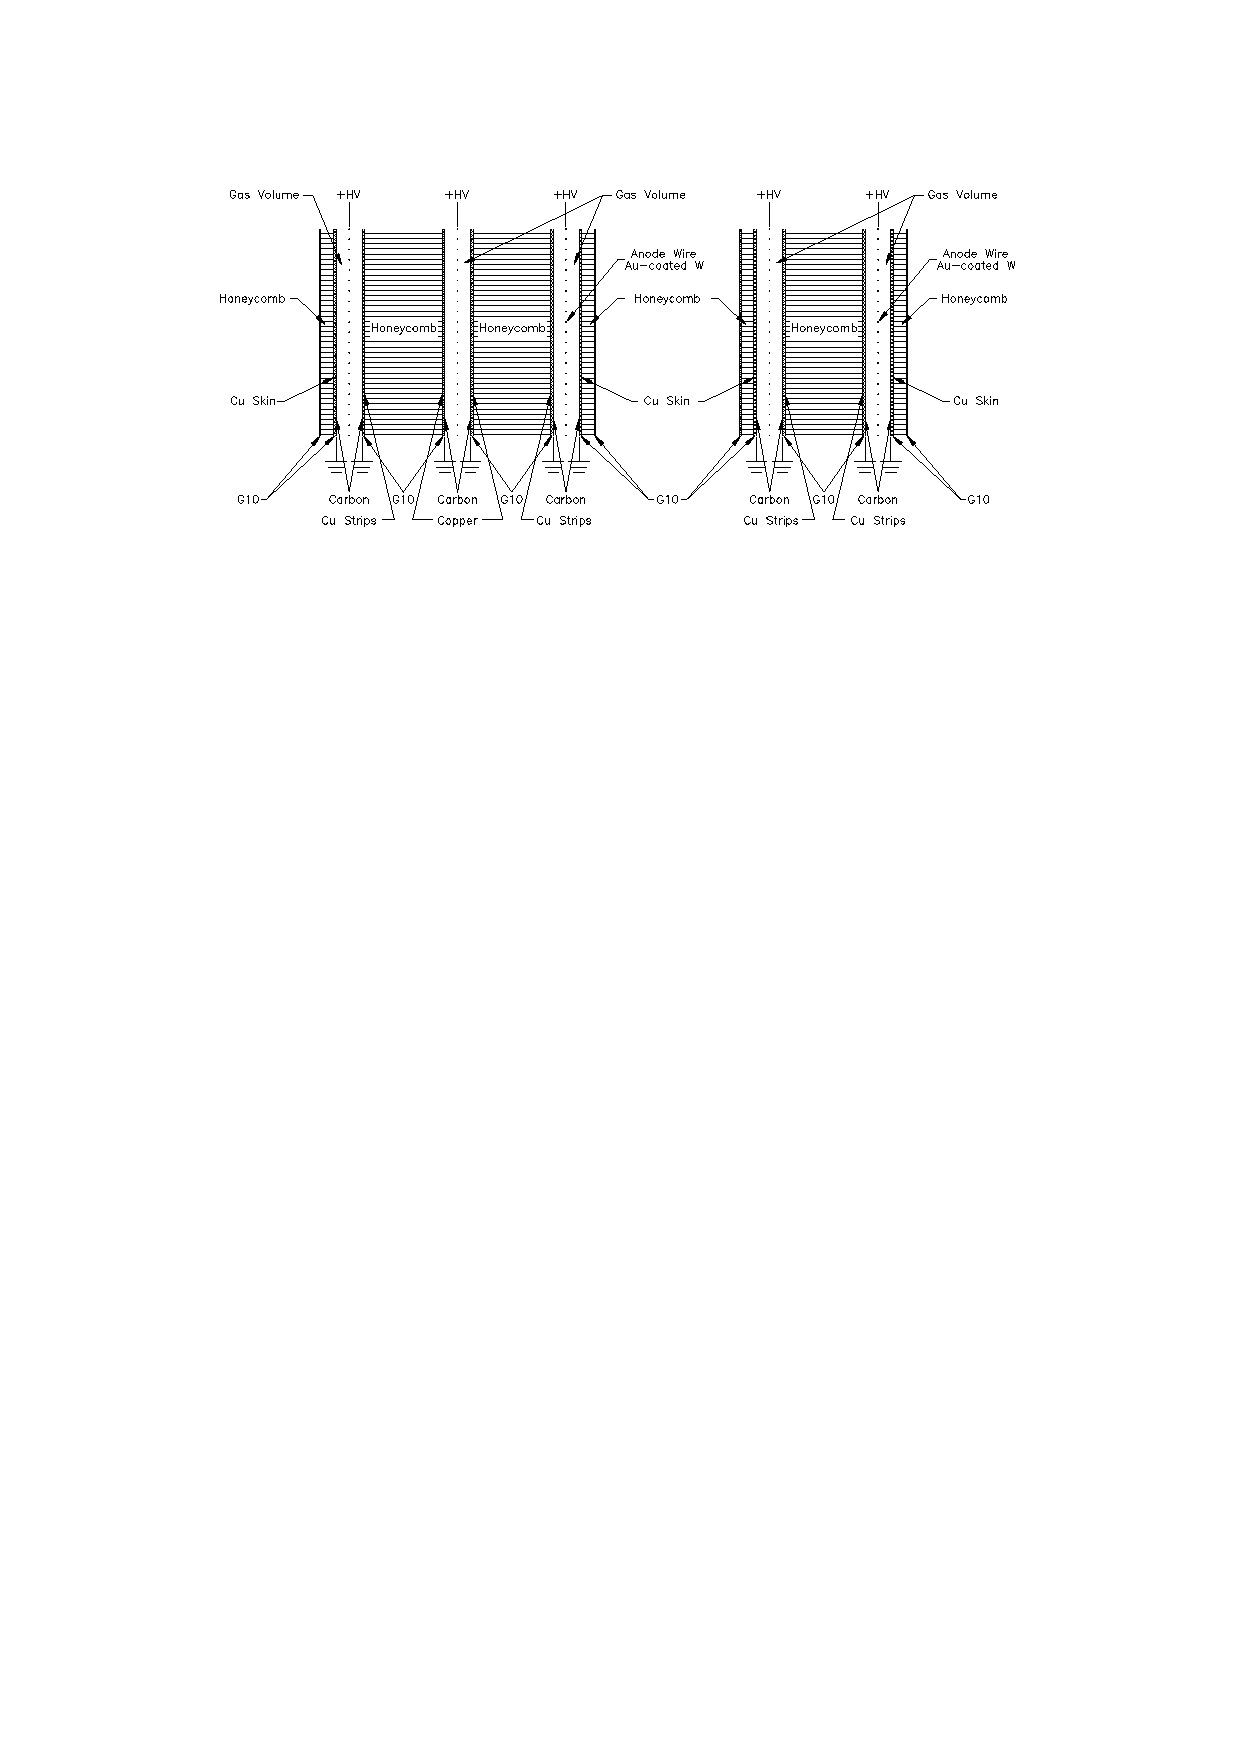
\includegraphics[height=5cm]{fig/Intro/TGC_crosssection.pdf}
\subcaption{TGC doubletとtripletの断面図}
\end{minipage}%
\caption[TGCチェンバーの断面図]{ (a)はTGCチェンバーの断面図を表す\cite{JINST:2008}。ワイヤーとストリップが直交して張られていることがわかる。 (b)はTGC doubletとtripletの断面図である。それぞれ2層、3層のガスギャップで構成されており、各ガスギャップの間はペーパーハニカムにより満たされている。}
\label{TGC_structure}
\end{figure}

TGC検出器はトリガー用の検出器であり、ワイヤー間隔が小さいため時間応答がよい。これにより陽子衝突頻度である25 nsより細かな時間分解能でミューオンを検出し、そのミューオンがどの陽子バンチ交差に由来するのかを識別 ( Bunch Crossing IDentification, BCID) することができる。一方、TGC検出器はそれほど高い位置分解能が求められていないため、ワイヤー電極を4 $\sim$ 20本まとめてから読み出しを行う。結果としてワイヤー、ストリップは合計32万チャンネルをもつ。

図\ref{TGC_picture}にTGC BWの写真を示す。BWの外側の領域 (1.05 < |$\eta$| < 1.92) はエンドキャップ領域、内側の領域  (1.92 < |$\eta$|< 2.4) はフォワード領域と呼び、異なる構造を取っている。エンドキャップ領域では$\phi$方向に48 回対称になるように、フォワード領域では$\phi$方向に24 回対称になるようにチェンバーが設置されている。エンドキャップ領域の 1/48、フォワード領域の 1/24 はトリガー回路的に独立しており、それぞれが"トリガーセクター"と呼ばれる。
また、電源供給、ガス供給、電気回路制御、読み出しの観点からBWは$\phi$方向に 12 個のセクターに分割されており、これを 1/12 セクターと呼ぶ。
\begin{figure} 
    \centering
    \includegraphics[width=14cm]{fig/Intro/TGC_picture.pdf}
    \caption[TGC検出器]{TGC検出器の正面写真 ( M1 )\cite{cern_document_server}。TGC検出器は電源供給、ガス供給、電気回路制御、読み出しの観点から$\phi$方向に 12 回対称になっており、赤枠で囲った範囲を 1/12 セクターと呼ぶ。また、TGC検出器は$\eta$方向に2種類の構造をとっており、円盤の外側の領域  (1.05 < |$\eta$| < 1.92) をエンドキャップ領域、円盤の内側の領域  (1.92 < |$\eta$|< 2.4) をフォワード領域と呼ぶ。エンドキャップ領域では$\phi$方向に 48 回対称になるよう、フォワード領域では$\phi$方向に 24回 対称になるようにチェンバーが設置されている。}
    \label{TGC_picture}
\end{figure}



\section{TDAQシステムとPhase\two アップグレード}
\label{sec_TDAQ}
    LHCでは 25 nsの間隔で陽子バンチが衝突するため、衝突で生じたすべてのデータを保存することはできない。限られた読み出し帯域とオフラインの計算リソースを最大限有効活用するためには興味のある衝突事象のみを記録するトリガーが重要となる。またトリガー判定がなされたイベントに対して正しくデータを取得するには、トリガーシステムとデータ取得 (data acquisition、DAQ) システムが連動して機能する必要がある。ATLAS実験では、トリガーとデータ取得をまとめてTrigger and Data Acquisition (TDAQ) システムと呼ぶ。本節ではRun 3 でのTDAQシステムとPhase\two でのTDAQシステムについて説明し、Phase\two アップグレードにおける変更点を述べる。
   
    \subsection{Run 3でのTDAQシステム}
    \label{subsec_run3TDAQ}
    図\ref{Run3_TDAQ}にRun 3におけるTDAQシステムの概要を示す。ATLASのトリガーシステムはLevel-1という初段のハードウェアトリガーと、それに続くHigh Level Trigger (HLT) という後段のソフトウェアトリガーから構成される。

    \begin{figure} 
    \centering
    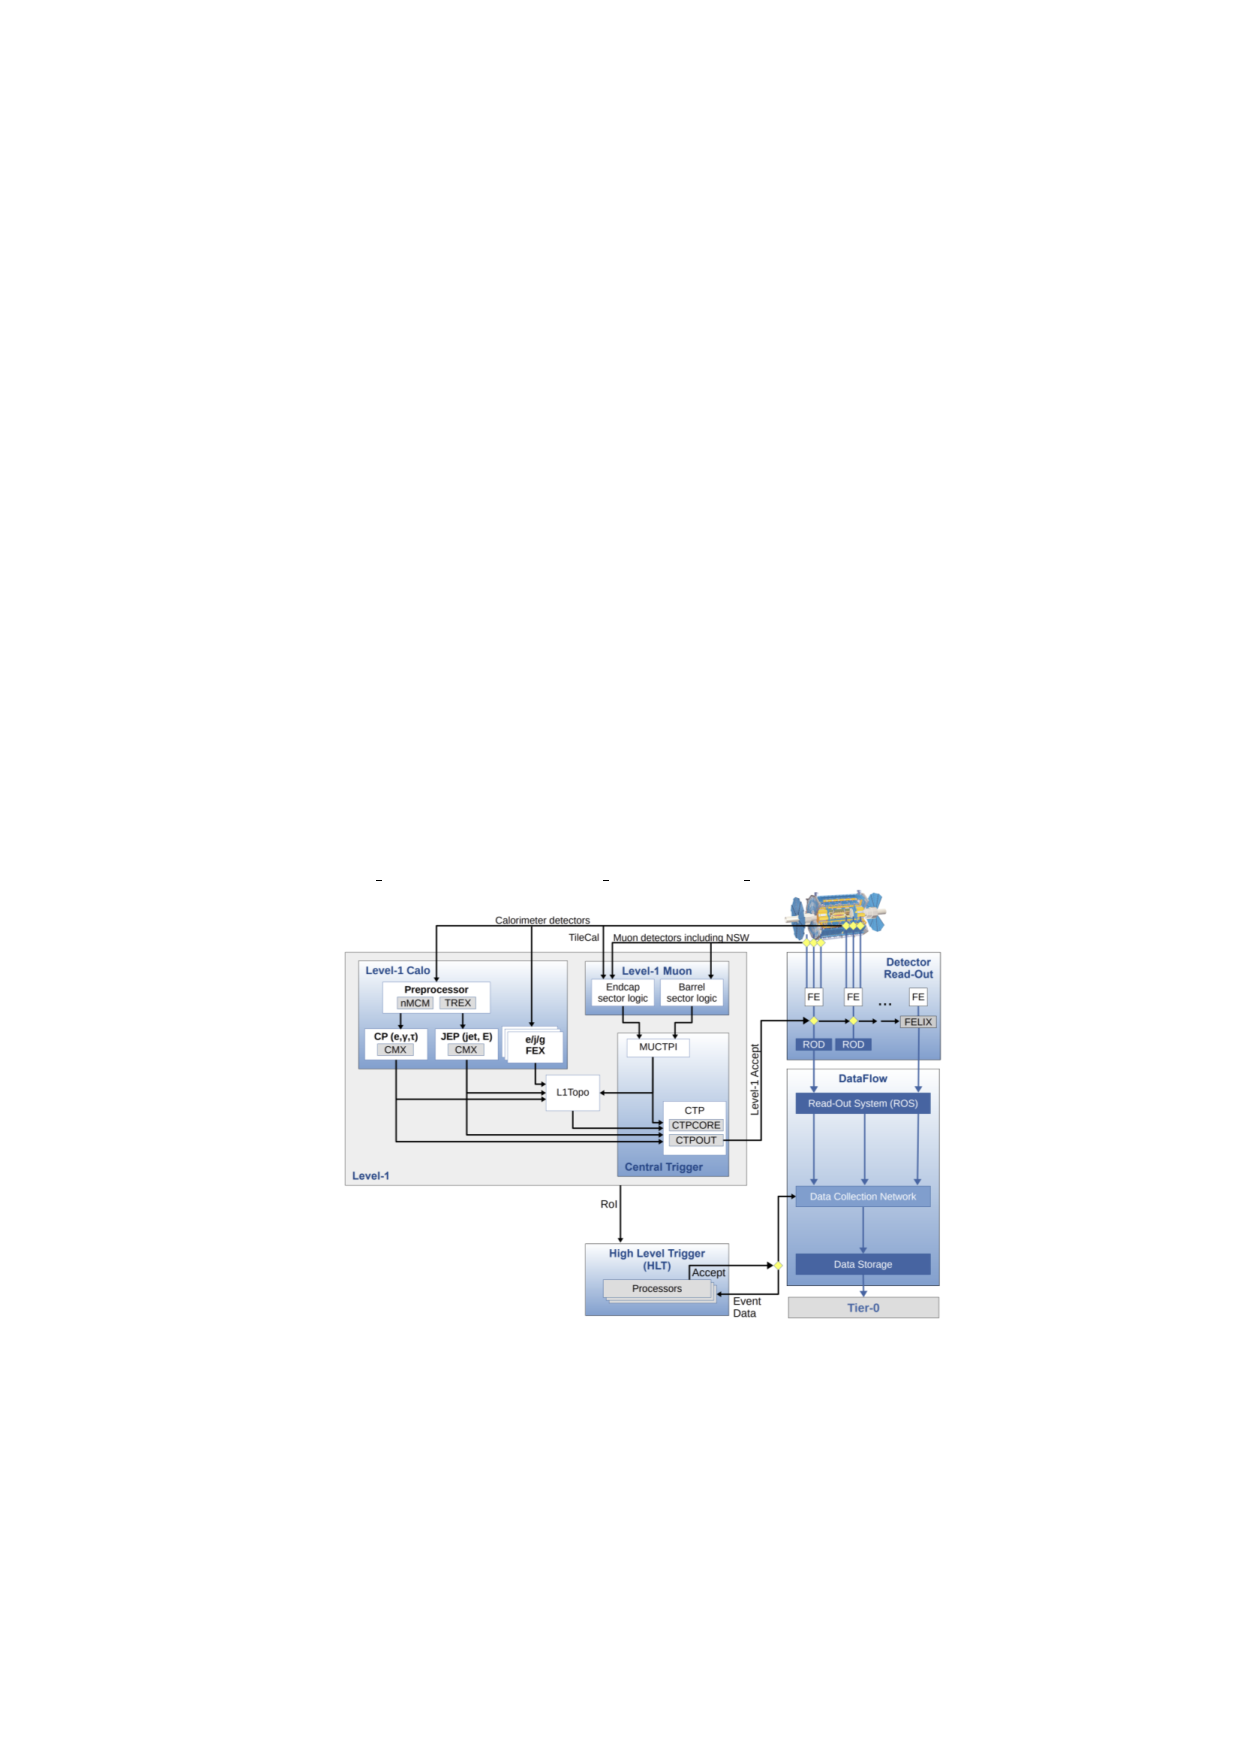
\includegraphics[width=16cm]{fig/Intro/Run3_TDAQ.pdf}
    \caption[Run 3におけるTDAQシステムの概要]{Run 3におけるTDAQシステムの概要\cite{Run3_TDAQ}。トリガーシステムはLevel-1 Triggerという初段ハードウェアトリガーとHigh Level Trigger (HLT)という後段のソフトウェアトリガーから構成される。L1 TriggerはLevel-1 CaloとLevel-1 Muonに大別されCTPで総合的なトリガー判定がなされる。L1 TriggerをパスしたイベントはHLTでより精度の高いトリガー判定が行われ、CERN Permanent Storageに保存される。 }
    \label{Run3_TDAQ}
    \end{figure}

    \subsubsection{Level-1 Trigger}
    \vskip0.5\baselineskip
    Level-1 Triggerは 25 ns間隔で行われるすべての陽子バンチ交差の中から、物理的に興味のある衝突事象を高速で選別する初段トリガーである。L1 Trigger 判定に従い、40 MHzの陽子バンチ交差に対して100 kHzまでのレートでデータが読み出される。L1 Triggerは全ての衝突のデータを処理し、トリガー判定を行う必要があるため、ASICやFPGAなどのハードウェアを利用し、高速処理を実現する。

    ATLASでのL1 Triggerシステムは主にカロリメータートリガー (Level-1 Calo) と ミューオントリガー (Level-1 Muon) で構成される。Level-1 Caloはカロリーメーターからのエネルギー情報をもとに、高いエネルギーを持つ電子、光子、ジェットを検出する。Level-1 MuonはRPCとTGCからの情報をもとに、横方向運動量の大きなミューオンを検出する。RPCとTGCからのトリガー情報はMUon-to Central Trigger Processor Interface (MUCTPI) で統合される。Level-1 CaloとLevel-1 Muonからの信号はCentral Trigger Processor (CTP) に渡され、総合的にLevel-1トリガー判定が行われる。L1 Triggerによって選別されたイベントについては、各検出器のフロントエンド回路にLevel-1 Accept (L1A) が送られ、そのバンチ交差に由来する検出器のヒット信号がReadout Driver (ROD) へと送られる。

    Level-1 Triggerではバンチ交差が生じてからL1Aが届けられるまでの時間 (Level-1 レイテンシー) が一定であるFIxed Latency Schemeを採用している。L1Aが出されるまでの間、陽子バンチ交差で生じるデータは各フロントエンドエレクトロニクス上のバッファーに保管される。現行システムではL1 レイテンシーは2.5 $\mu\mathrm{s}$に設定されており、それを満たすようフロントエンドエレクトロニクスの設計が行われている。

    \subsubsection*{High Level Trigger (HLT) }
    \vskip0.5\baselineskip
    HLTは初段トリガーをパスしたイベントから最終的にストレージに保存する事象を選ぶ役割を担う、ソフトウェアベースのトリガーである。初段トリガーでは使われなかった内部飛跡検出器やMDTなどの精密測定用検出器からの情報も利用して、より高い精度でイベント再構成を行う。HLTによりトリガーレートは3.3 kHzまで削減され、トリガーをパスしたイベントは、データセンターのストレージに記録される。その後CERNのコンピューティングセンターであるTier-0において処理され、イベントが再構成される。

    \subsubsection*{トリガーメニュー}
    ATLAS実験は陽子陽子衝突で生じるさまざまな事象を取得することで、幅広い終状態を持つ多様な物理解析を展開する。広範な物理事象を取得するため、複数のトリガー選別条件が用意されており、それぞれに適切なトリガーレートが分配されている。図\ref{Run2_Triggermenu}にトリガーメニューと呼ばれる、各トリガー選別条件とそれに割り振られたトリガーレートをまとめたリストを示す。
    トリガーメニューでは、解析で利用されるlepton、jet、消失横方向エネルギー ($E_\mathrm{T}^{\mathrm{miss}}$)などの典型的なオブジェクトを取得するための、Level-1およびHLTトリガー閾値が定められている。

    \begin{figure} 
    \centering
    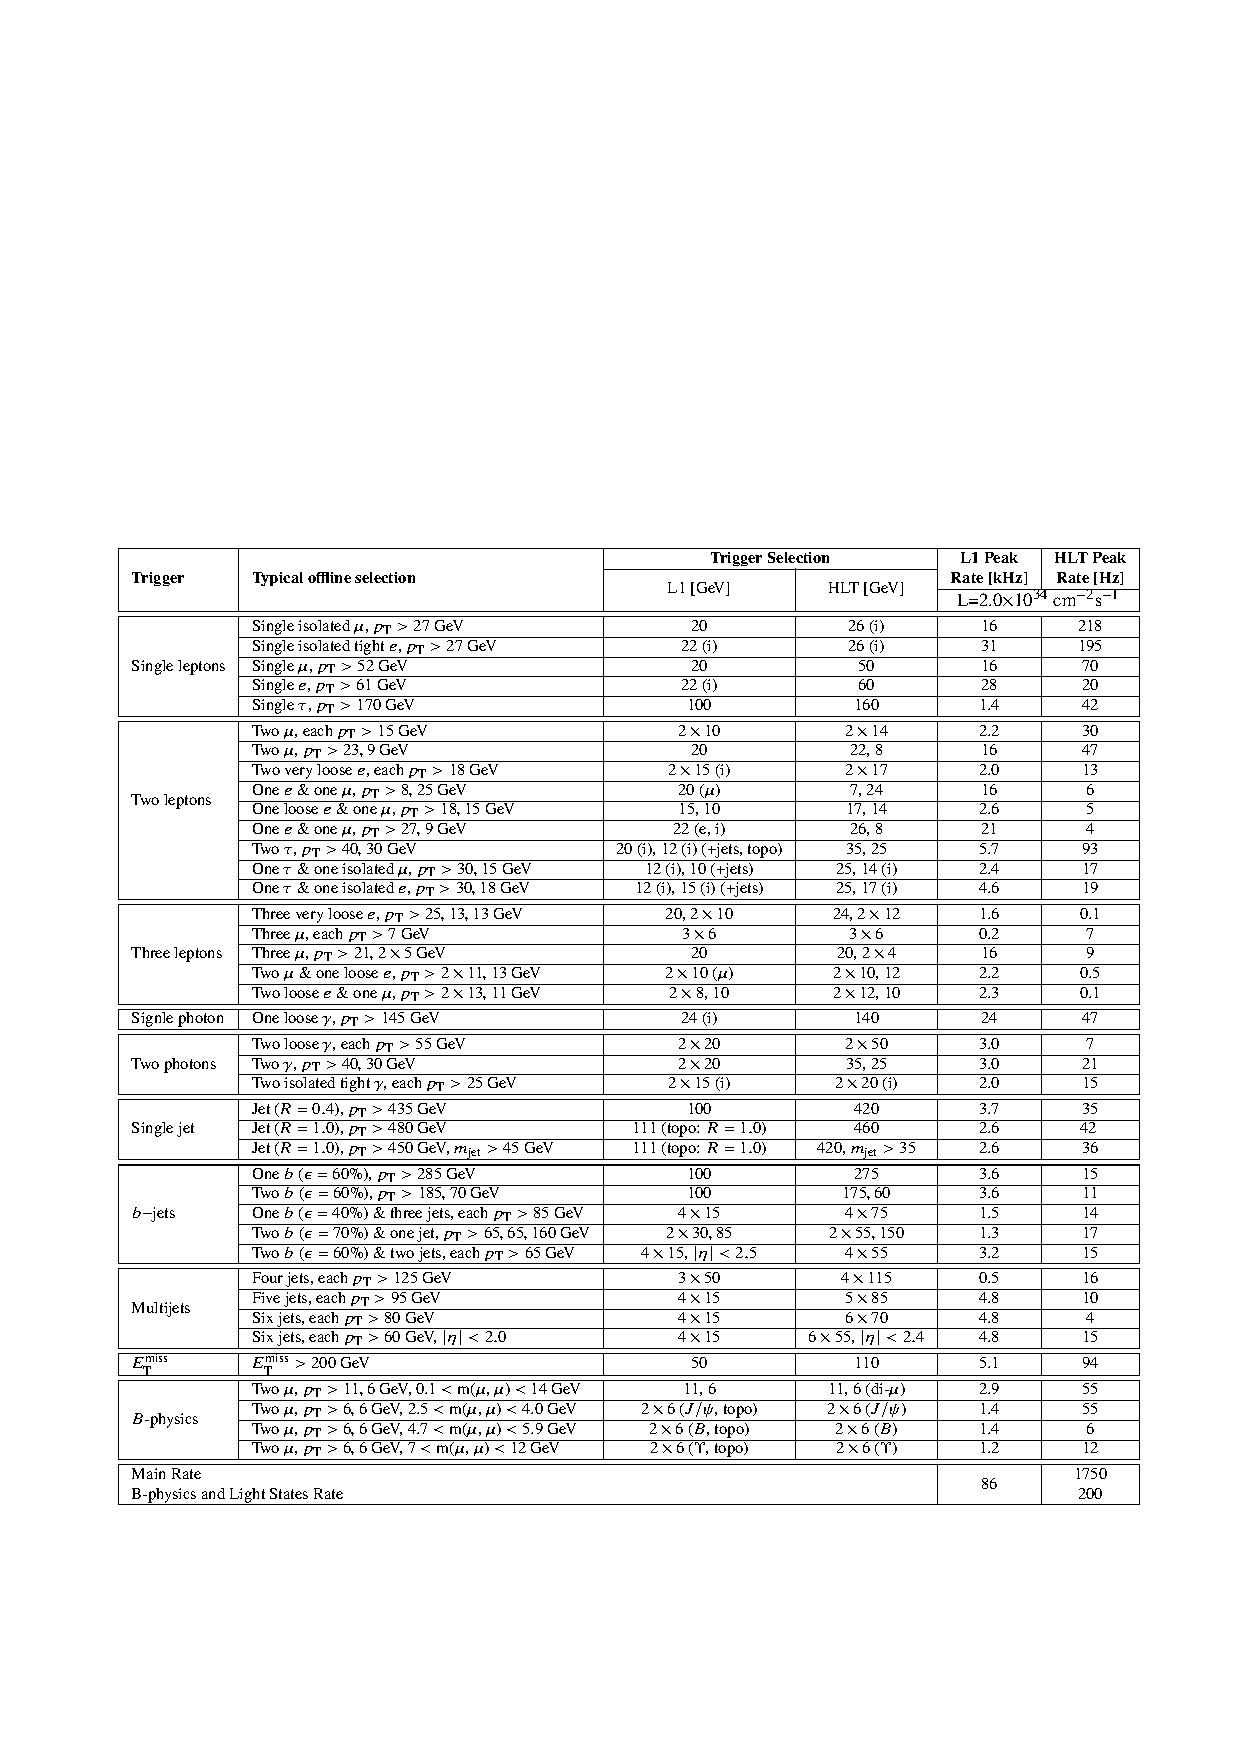
\includegraphics[width=16cm]{fig/Intro/Run2_Triggermenu.pdf}
    \caption[Run2でのトリガーメニューの一例]{Run2でのトリガーメニューの一例\cite{Run2_Triggermenu}。解析で利用される典型的なオブジェクトを取得するためのLevel-1およびHLTでのトリガー閾値が定められる。全体を通してトリガーレートの制約を守るよう設計される。}
    \label{Run2_Triggermenu}
    \end{figure}

    \subsection{高輝度LHC-ATLAS実験でのTDAQシステム}
高輝度LHC-ATLAS実験ではパイルアップによる背景事象が大幅に増加し、トリガーレートが増加する。現行のTDAQシステムのままでは、読み出し能力の限界からトリガー制約を厳しくせざるを得ず、その結果、興味のある物理事象へのアクセプタンスを落としてしまう。そこで高輝度LHC-ATLAS実験に向けて、大規模なTDAQシステムのアップグレードが行われる。初段トリガーレートは 100 kHzから 1 MHzへ、後段トリガーレートは 3.3 kHzから 10 kHzへと拡張される。さらに、初段トリガーレイテンシーも 2.5 $\mu\mathrm{s}$から 10 $\mu\mathrm{s}$へと拡張される。図\ref{Phase2_TDAQ}に高輝度LHC-ATLAS実験でのTDAQシステムの概要を示す。
高輝度LHC-ATLAS実験では初段トリガーをLevel-0 Trigger、後段トリガーをEvent Filter (EF) と呼ぶ。

\begin{figure}
\begin{minipage}[b]{.5\linewidth}
\centering
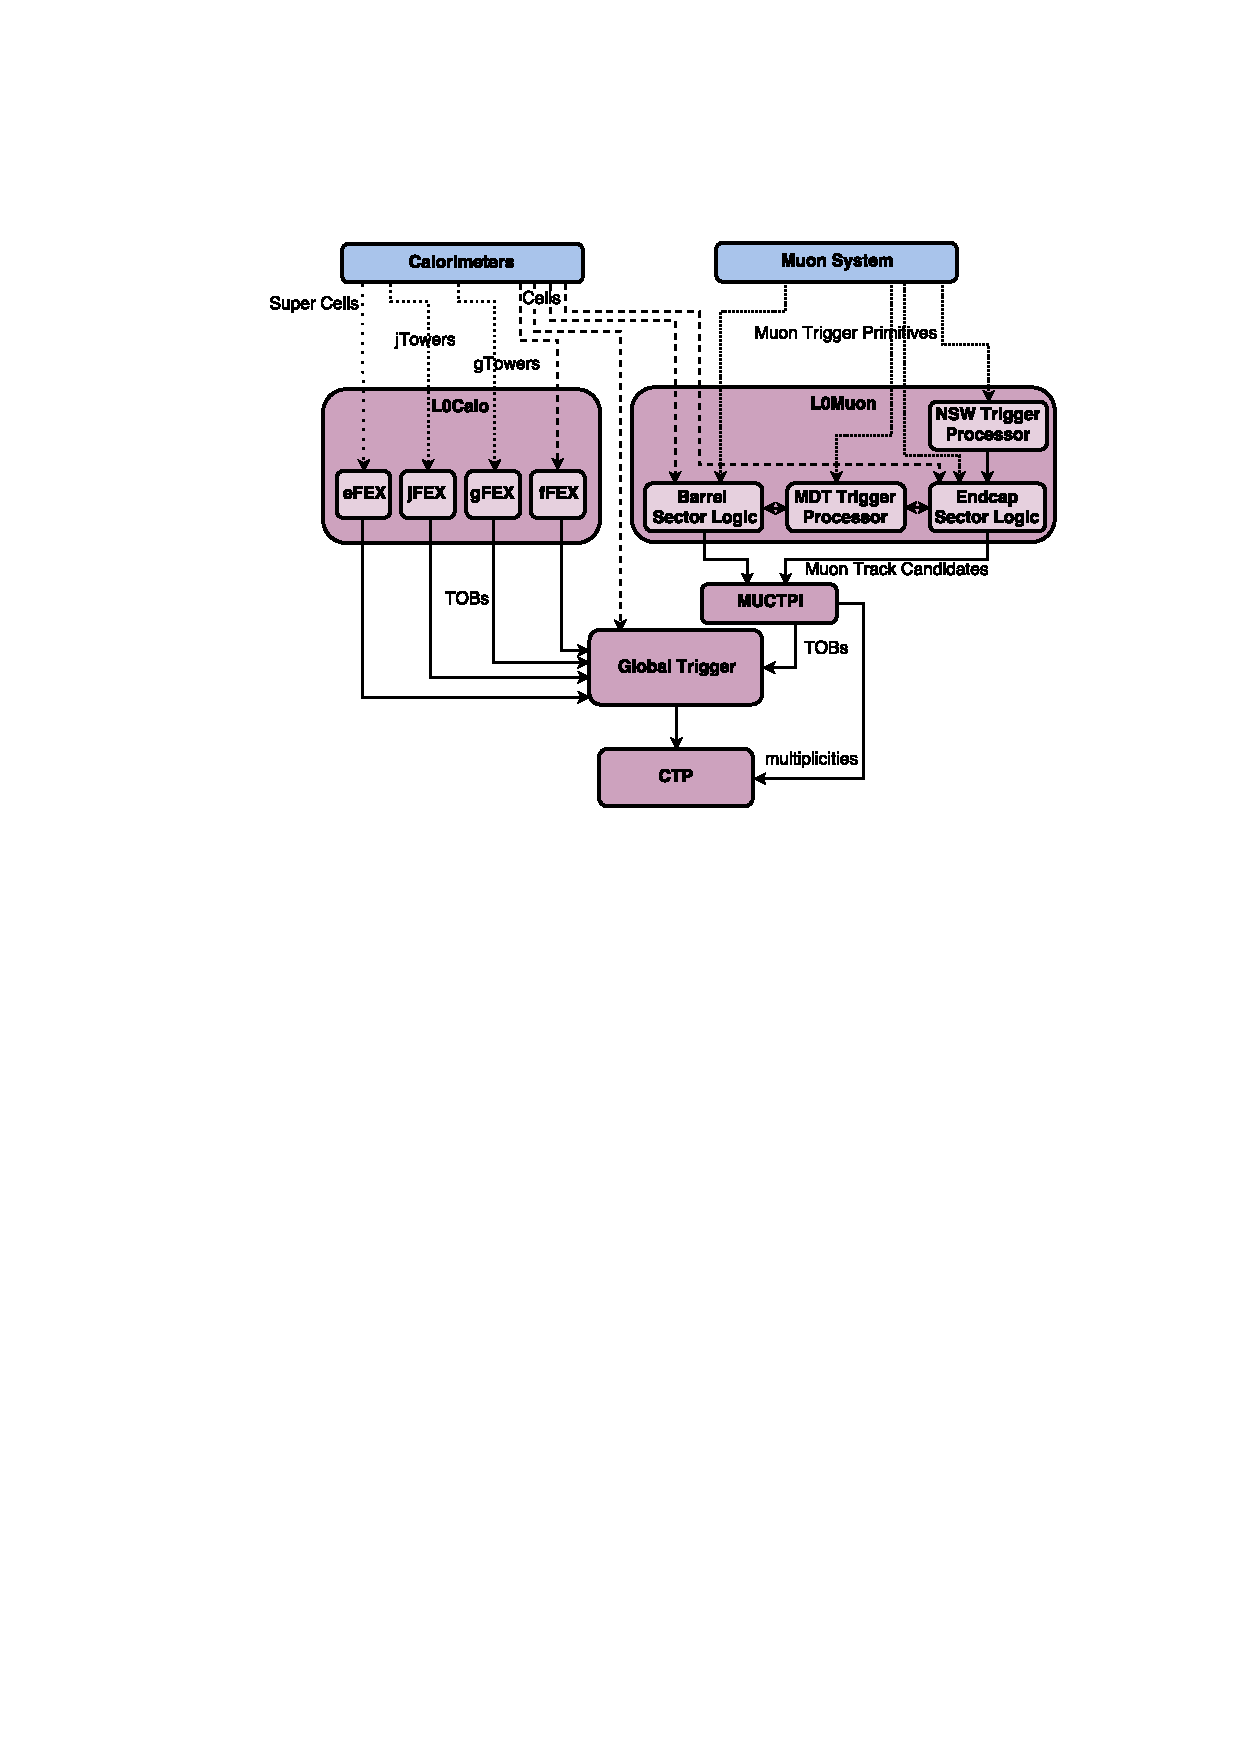
\includegraphics[height=6.5cm]{fig/Intro/Phase2_L0trigger.pdf}
\subcaption{Level-0 Triggerシステムの概要}
\end{minipage}%
\begin{minipage}[b]{.5\linewidth}
\centering
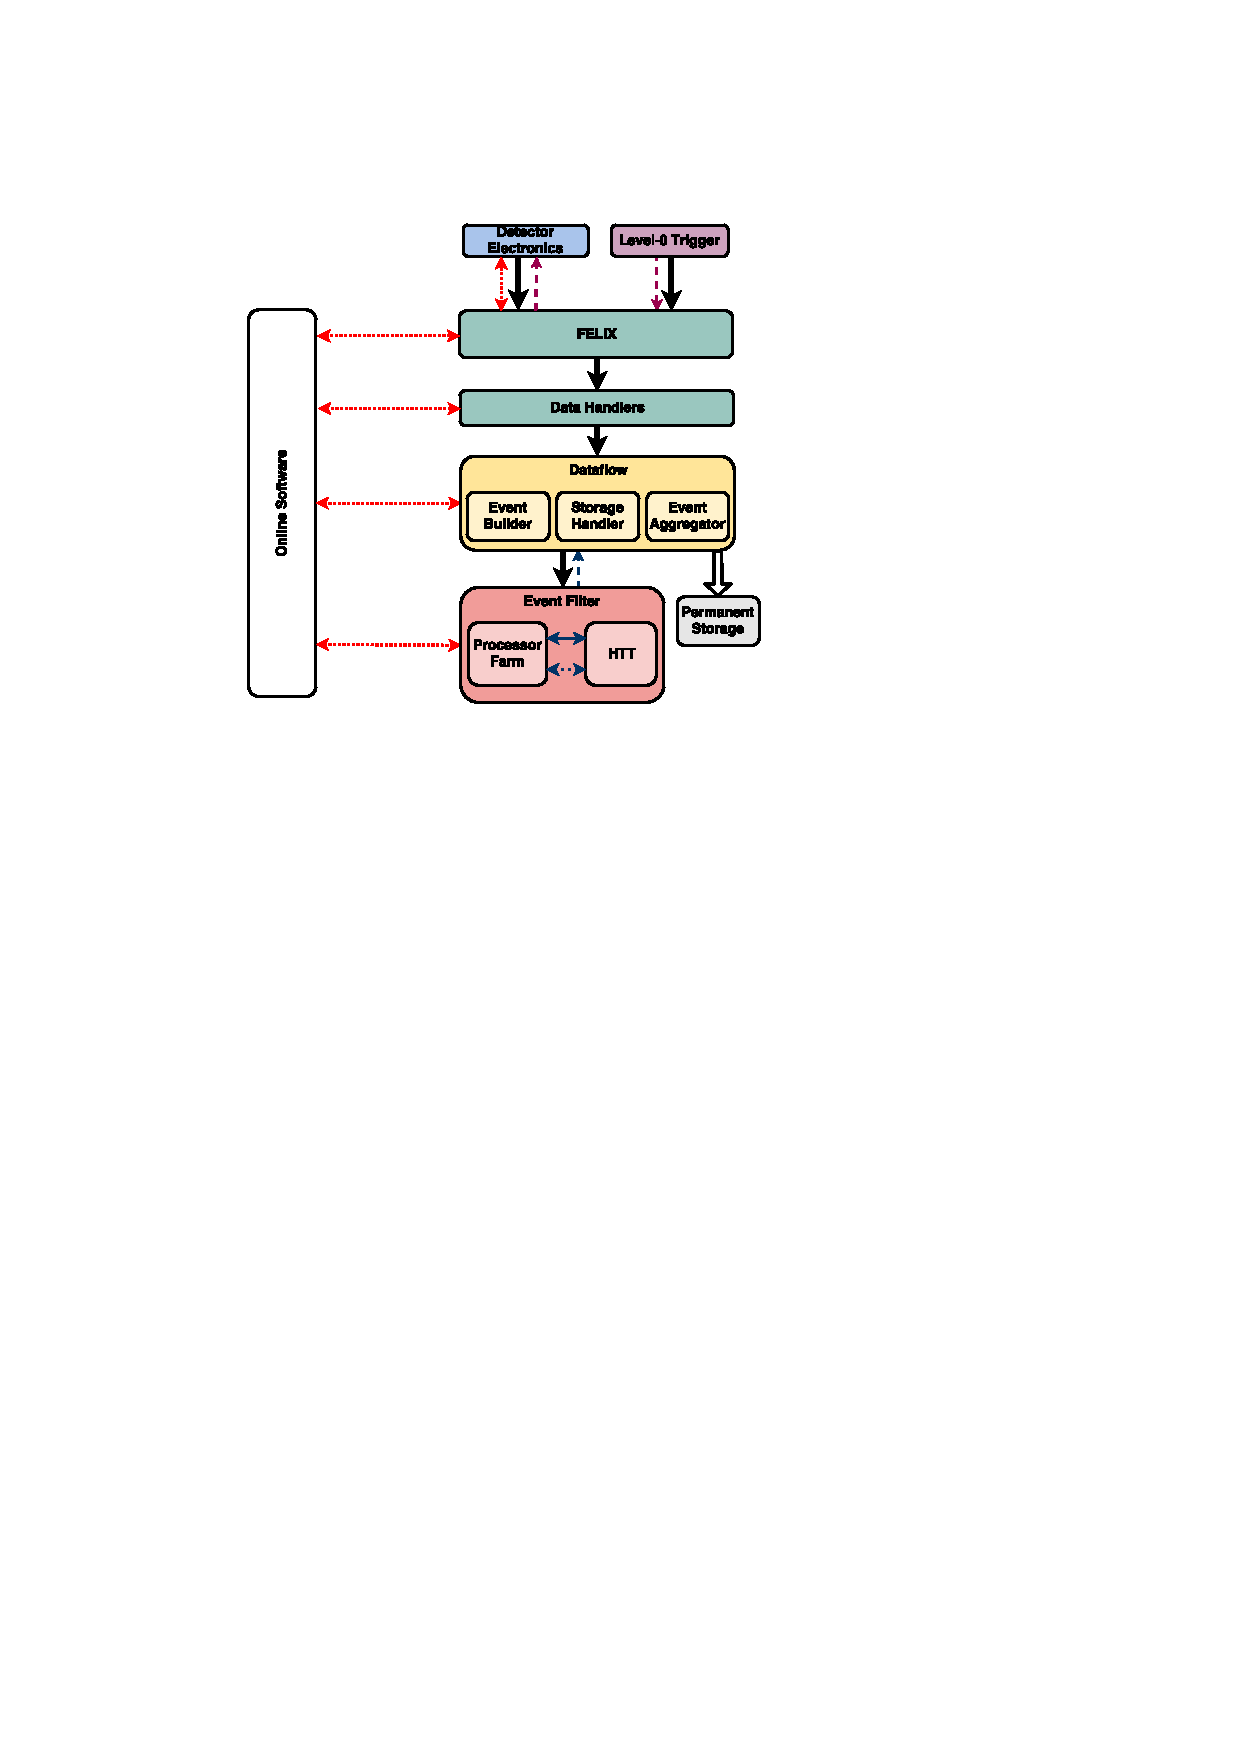
\includegraphics[height=6.5cm]{fig/Intro/Phase2_EF.pdf}
\subcaption{Event FilterとDAQシステムの概要}
\end{minipage}%
\caption[高輝度LHC-ATLAS実験におけるTDAQシステムの概要]{高輝度LHC-ATLAS実験におけるTDAQシステムの概要\cite{tdr_phase2tdaq_2017020}。 (a)にLevel-0 Triggerシステムの概要を示す。Level-0 TriggerはLevel-0 CaloとLevel-0 Muonに大別され、CTPで総合的なトリガー判定がなされる。CTPで後段に送られるべきと判断された場合、FELIXを経由して各フロントエンドエレクトロニクスにL0A信号が分配される。 (b)にEvent FilterとDAQシステムの概要を示す。L0Aを受けた各システムは検出器からのヒットデータをFELIXに送る。FELIXは受け取ったデータをEvent Filterに渡す。EFではソフトウェアベースのトリガー判定が行われ、最後まで残ったデータがCERNのPermanent Strageに保存される。}
\label{Phase2_TDAQ}
\end{figure}

L0 TriggerはL0 Calo、L0 Muon、Global Trigger、CTPで構成される。L0 Muonでは、新たに精密測定用のMDTもトリガーに用いられるようになる。TGCやRPCの情報と組み合わせることで、より精度の高いトリガー判定を実現する。Global TriggerはL0 CaloとMUCTPIからの位置や\pt、\Et などの情報を基に、特徴的なトポロジーを持つ事象か判断し、その結果をCTPに送る。CTPはL0 Calo、L0 Muon、L0 Globalからの入力に基づき、トリガーメニュー (図\ref{Phase2_Triggermenu}) に従い、各トリガー条件に指定されたプリスケーリングファクターを適用してトリガー判定を行う。各フロントエンドエレクトロニクスにはFront-End Link eXchange  (FELIX) を経由してLevel-0 Accept (L0A) 信号が分配される。L0Aを受けた各エレクトロニクスは該当する陽子バンチ交差に由来する、データをFELIXに送信する。FELIXはこれらのデータをEvent Filterに転送する。Event Filterではソフトウェアベースのトリガー判定が行われ、トリガーレートは10 kHzまで削減される。最終的に残った生データは、CERNのデータセンターのストレージに保存される。

\begin{figure} 
\centering
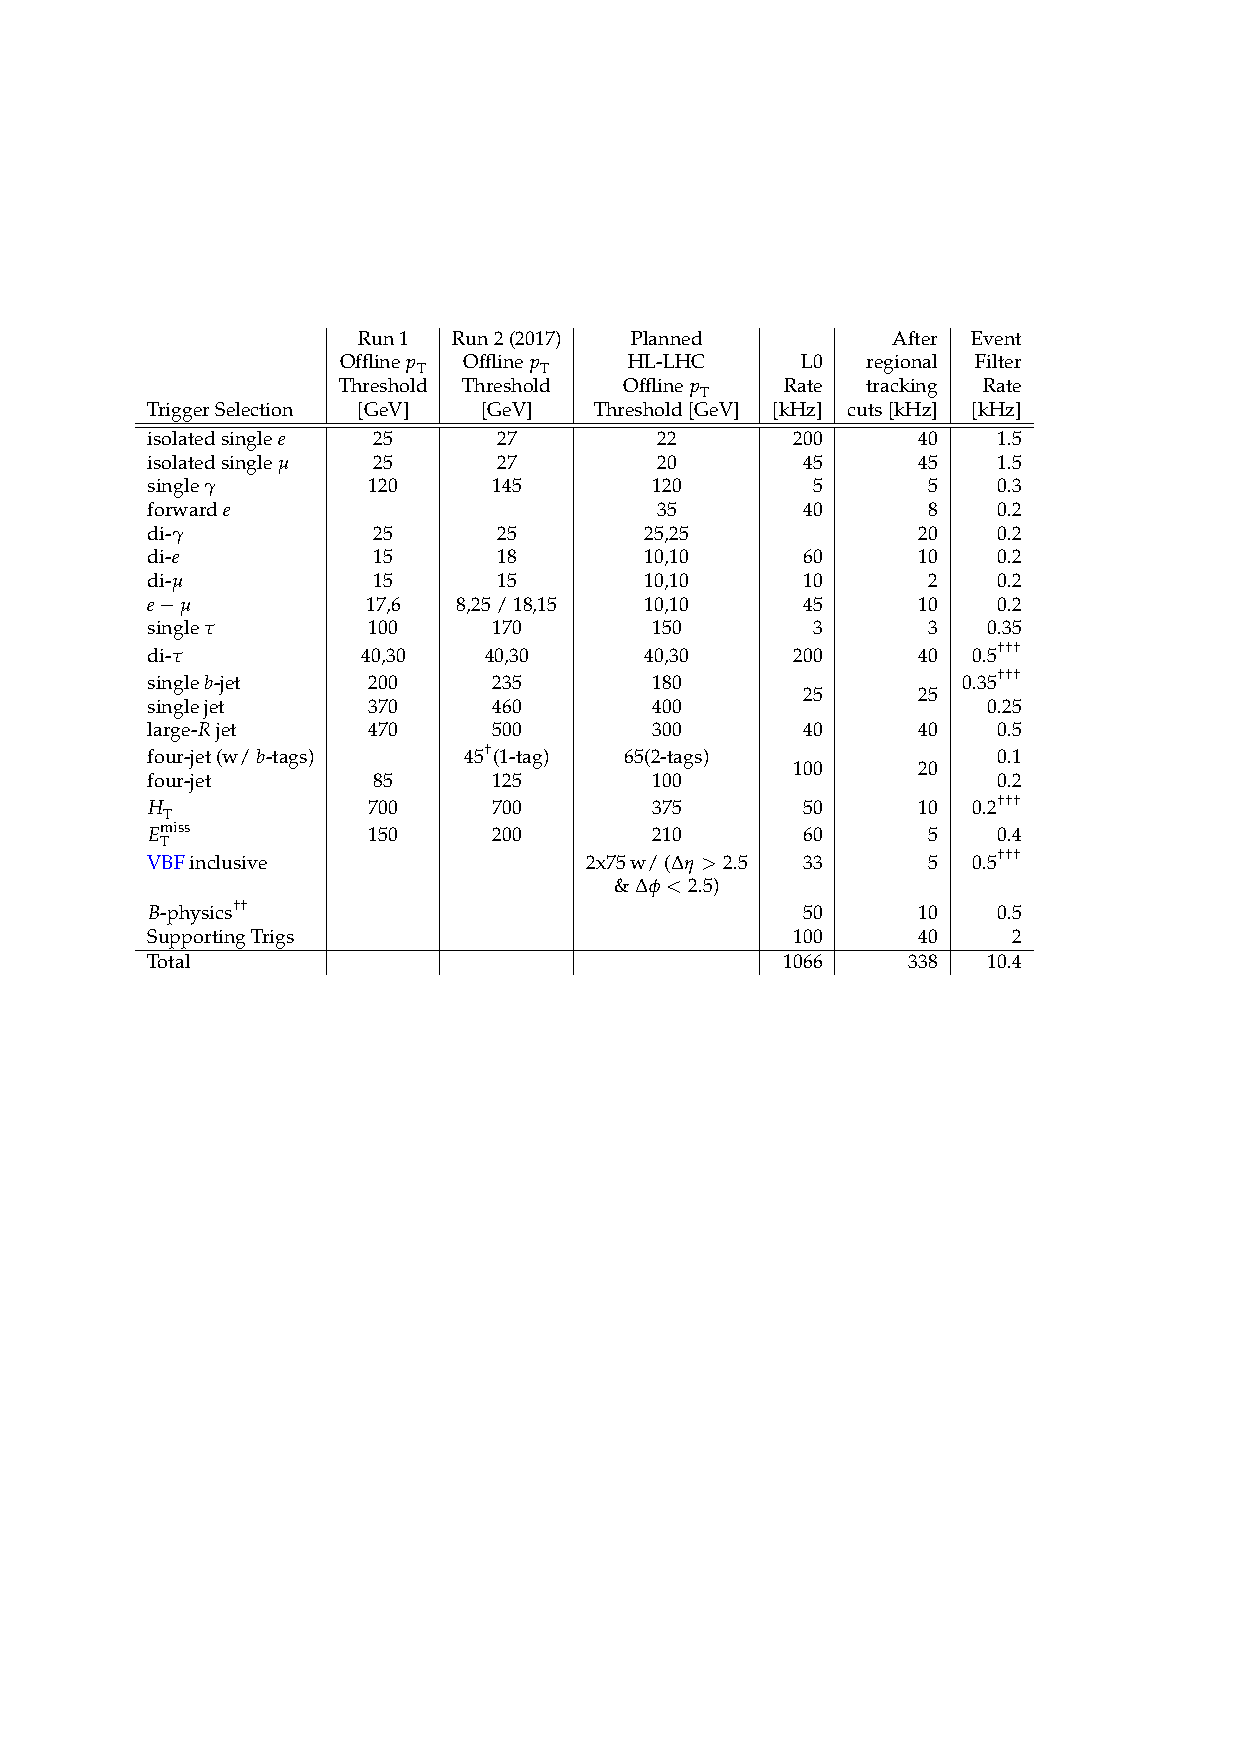
\includegraphics[width=16cm]{fig/Intro/Phase2_Triggermenu.pdf}
\caption[高輝度LHCにおけるトリガーメニューの例]{高輝度LHCにおけるトリガーメニューの例\cite{tdr_phase2tdaq_2017020}。解析に利用される典型的なオブジェクトに対してL0 TriggerおよびEvent Filterでのトリガーレートが分配されている。L0 TriggerレートはRun 3の約10倍、Event Filterでのレートは約6倍に増強される。}
\label{Phase2_Triggermenu}
\end{figure}

\section{TGC検出器の読み出し、トリガー、電気回路システムとPhase\two アップグレード}
\label{sec_TGCtrigger}
高輝度LHC-ATLAS実験に向けたTDAQシステムのアップグレードに伴い、TGC検出器の読み出し、トリガー、電気回路システムも大幅にアップグレードされる。本節ではまずTGC検出器におけるトリガーのコンセプトを説明する。次にRun 3 でのTGC検出器システムとPhase\two でのTGC検出器システムについて説明し、Phase\two アップグレードにおける変更点を述べる。

    \subsection{TGCトリガーのコンセプト}
    \label{subsec_trigger_concept}
衝突点からエンドキャップ方向  (1.05 < |$\eta$| < 2.4) に飛来するミューオンは、エンドキャップトロイド磁石で曲げられTGC検出器に入射する。TGC検出器の各層ではワイヤー、ストリップによる2次元読み出しで、TGCを通過したミューオンの  ($R$、$\phi$) 座標を検出する。TGC検出器は$z$方向に3つのステーションを持っており、ステーション間のコインシデンスをとることでミューオンの3次元飛跡を再構成し、それをもとに運動量を概算する。より具体的な運動量概算手法の概要を図\ref{TGC_triggerconcept}に示す。

\begin{figure} 
\centering
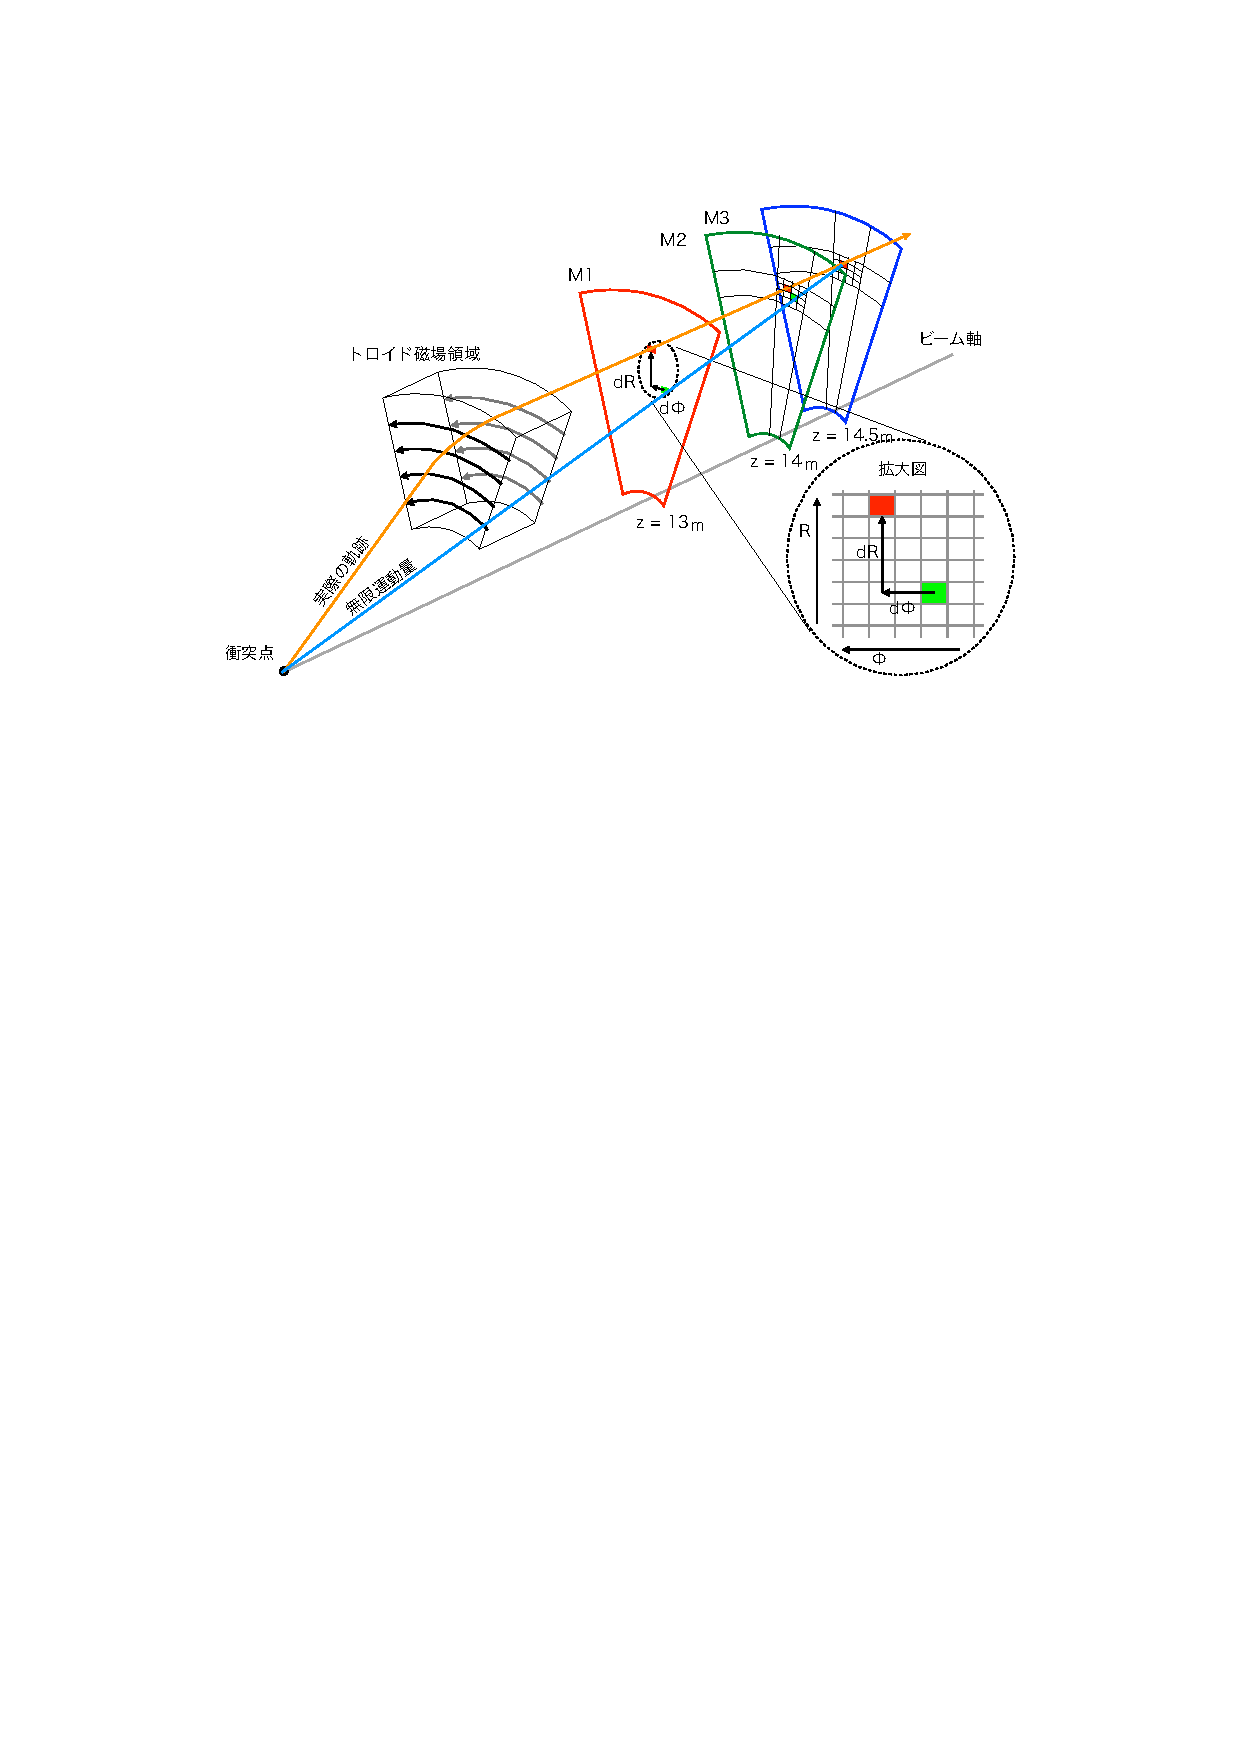
\includegraphics[width=16cm]{fig/Intro/TGC_triggerconcept.pdf}
\caption[TGCにおけるトリガーのコンセプト]{TGCにおけるトリガーのコンセプト\cite{mt_akatsuka}。ミューオンがTGCに残したヒット点から再構成した"実際の飛跡"と無限運動量飛跡の位置の差分 ($\mathrm{dR}$,$\mathrm{\phi}$)を利用して\pt を概算する。}
\label{TGC_triggerconcept}
\end{figure}

TGC検出器はエンドキャップトロイド磁場の外側に位置するため、ミューオンは検出器を直線的に通過する。TGC検出器では、3つのステーションのヒットから再構成したミューオンの飛跡 (図中の実際の飛跡) と、M3のヒット点 (ピボット) と衝突点を直線的結んだ"無限運動量飛跡"のなす角を分別変数に利用して、\pt を概算する。具体的にRun 3のロジックでは、ミューオンが実際に残したヒット点と無限運動量飛跡のM1およびM2の交点との位置の差分  ($\mathrm{d}R$ , $\mathrm{d}\phi$)を 利用する\footnote{高輝度LHC-ATLAS実験では実際の飛跡と無限運動量飛跡のなす角($\mathrm{\Delta\theta, \Delta\phi}$)が利用される。本質的に等価なロジックである。}。特に、ミューオンはエンドキャップトロイド磁場で主に$R$方向に曲げられるため、$\mathrm{d}R$は\pt と強い相関を持った値となる。一方、$\phi$方向にはあまり曲げられないため、衝突点から飛来するミューオンの$\mathrm{d\phi}$は\pt によらず小さい値を取る。そのため$\mathrm{d}\phi$は再構成したミューオン飛跡が、衝突点に由来するものであることを担保するために利用される。

\ref{subsec_magnet}節で述べたように、エンドキャップ領域に生成されるトロイド磁場は、$\phi$方向にも方向にも均一ではない上、その大きさも一様でない。そのため、($\mathrm{d}R$ , $\mathrm{d\phi}$)と\pt の関係はミューオンの飛来する場所に依存する複雑な関数となり、代数的にも電気回路的にも求めるのは難しい。そこでシミュレーションを用いて、あらかじめ  ($\mathrm{d}R$ , $\mathrm{d\phi}$) と\pt の関係性をまとめたテーブル  (Look Up Table、LUT) を領域ごとに用意することで、複雑な計算をすることなく、高速で\pt を計算する。この手法をパターンマッチングと呼ぶ。

上述したTGC BW のヒットデータのみを用いたトリガーロジックでトリガー判定を行なっていたRun 1では、フェイクトリガーと呼ばれる、衝突点に由来しない荷電粒子に対して誤ってトリガーを発行してしまう事象が多く発生していた。図\ref{TGC_faketrigger}にRun 1でのミューオントリガーをパスしたイベント数の$\eta$分布を示す。TGCがトリガーを担当する1.05 < |$\eta$|の領域では、オフラインで再構成されたミューオンイベントよりはるかに多くのイベントがトリガーをパスしていることがわかる。この差分の多くがフェイクトリガーによるものであると考えられる。フェイクトリガーの主な原因として、陽子陽子衝突や、ハドロンカロリメーター内で生じた中性ハドロンが、エンドキャップトロイド磁石の支持構造体と相互作用し荷電粒子を放出するケースが挙げられる。

この問題に対処するため、Run 2以降のトリガーではInner Coincidenceという新しいロジックが追加された。Inner Coincidenceの概要を図\ref{TGC_Inner_concept}に示す。Inner Coincidenceは、TGC検出器で再構成したミューオン飛跡と、エンドキャップトロイド磁石内部に設置された検出器で再構成したミューオン飛跡のマッチングをとるもので、これによって衝突点に由来する粒子とそうでないものを見分けることが可能となる。さらに、NSWなどの精密測定用の検出器で再構成された飛跡情報を組み合わせることで、TGC BW 単体での\pt 計算より精度を向上させることができる。


\begin{figure} 
\centering
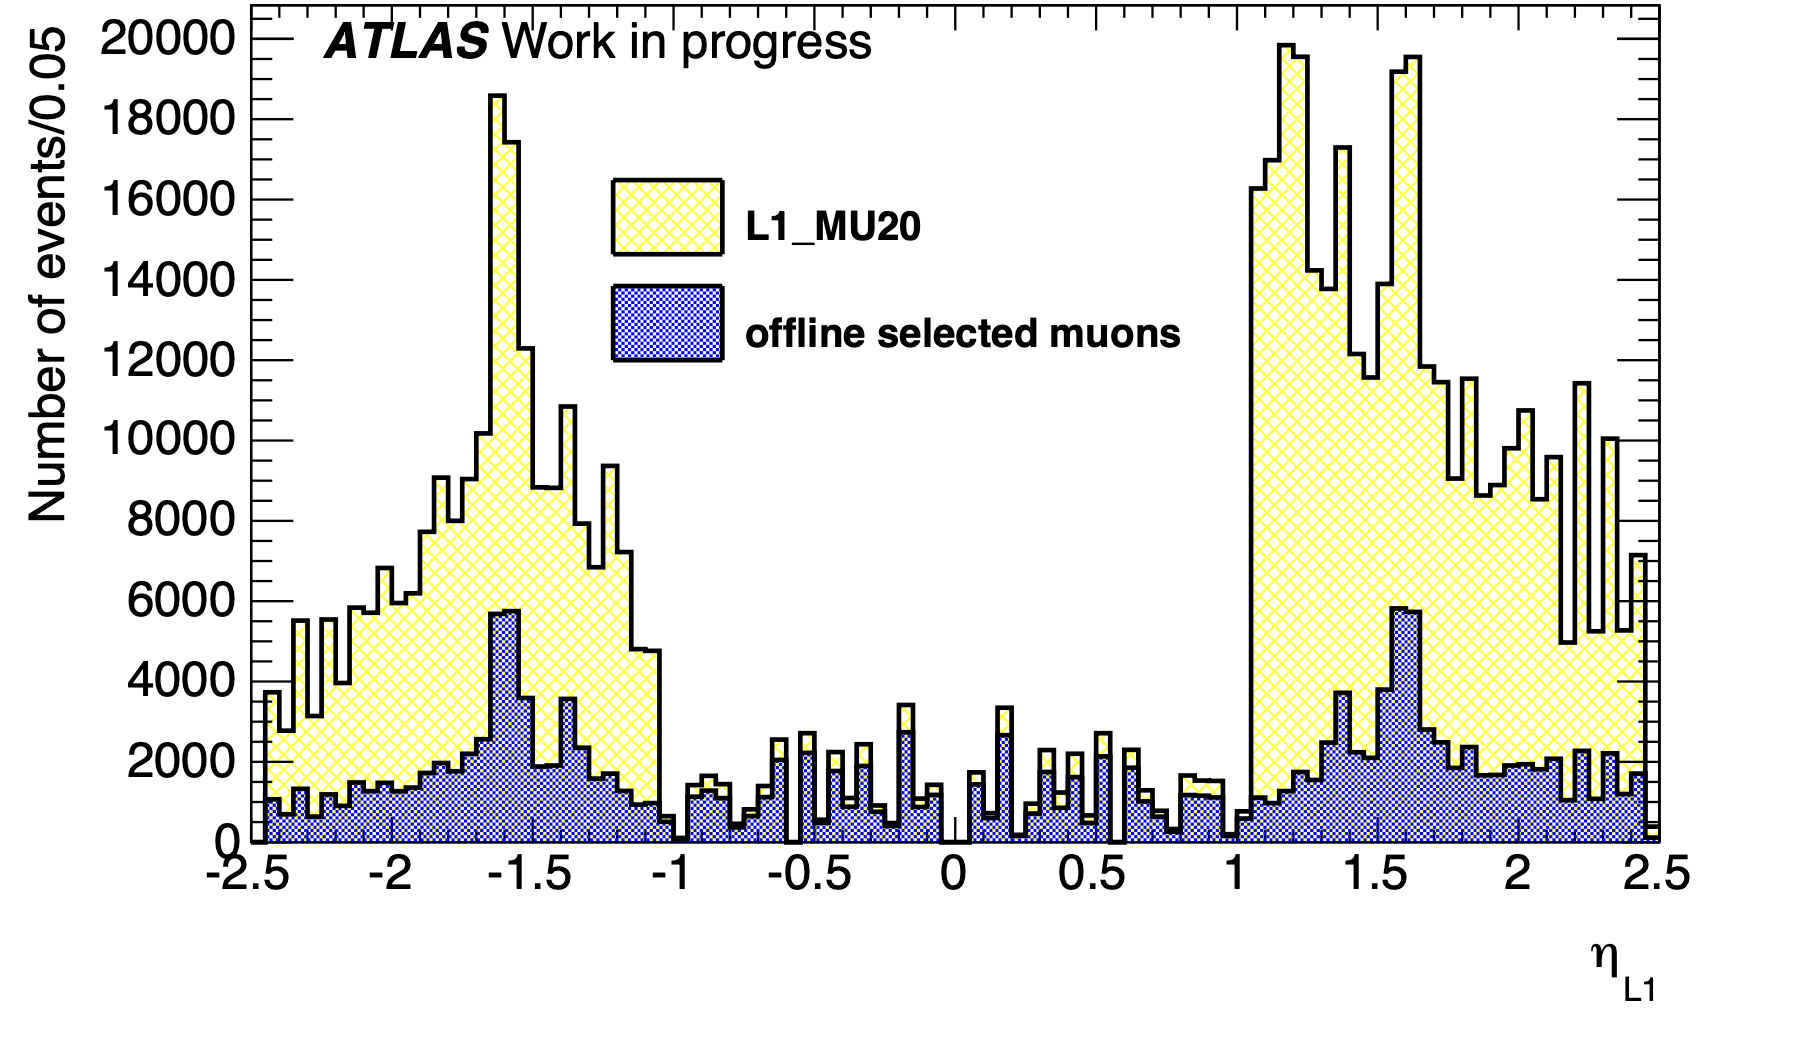
\includegraphics[width=16cm]{fig/Intro/TGC_faketrigger.png}
\caption[Run-1での\pt 閾値]{Run 1における、L1 Muonをパスしたイベント数とオフラインで再構成されたミューオンイベント数の比較。TGCがトリガーを担当する1.05 < |$\eta$|の領域で、オフラインで再構成されたミューオンイベント数より多くのイベントがミューオントリガーをパスしていることがわかる。この差分がフェイクトリガーによるものと考えられる。}
\label{TGC_faketrigger}
\end{figure}

\begin{figure} 
    \centering
    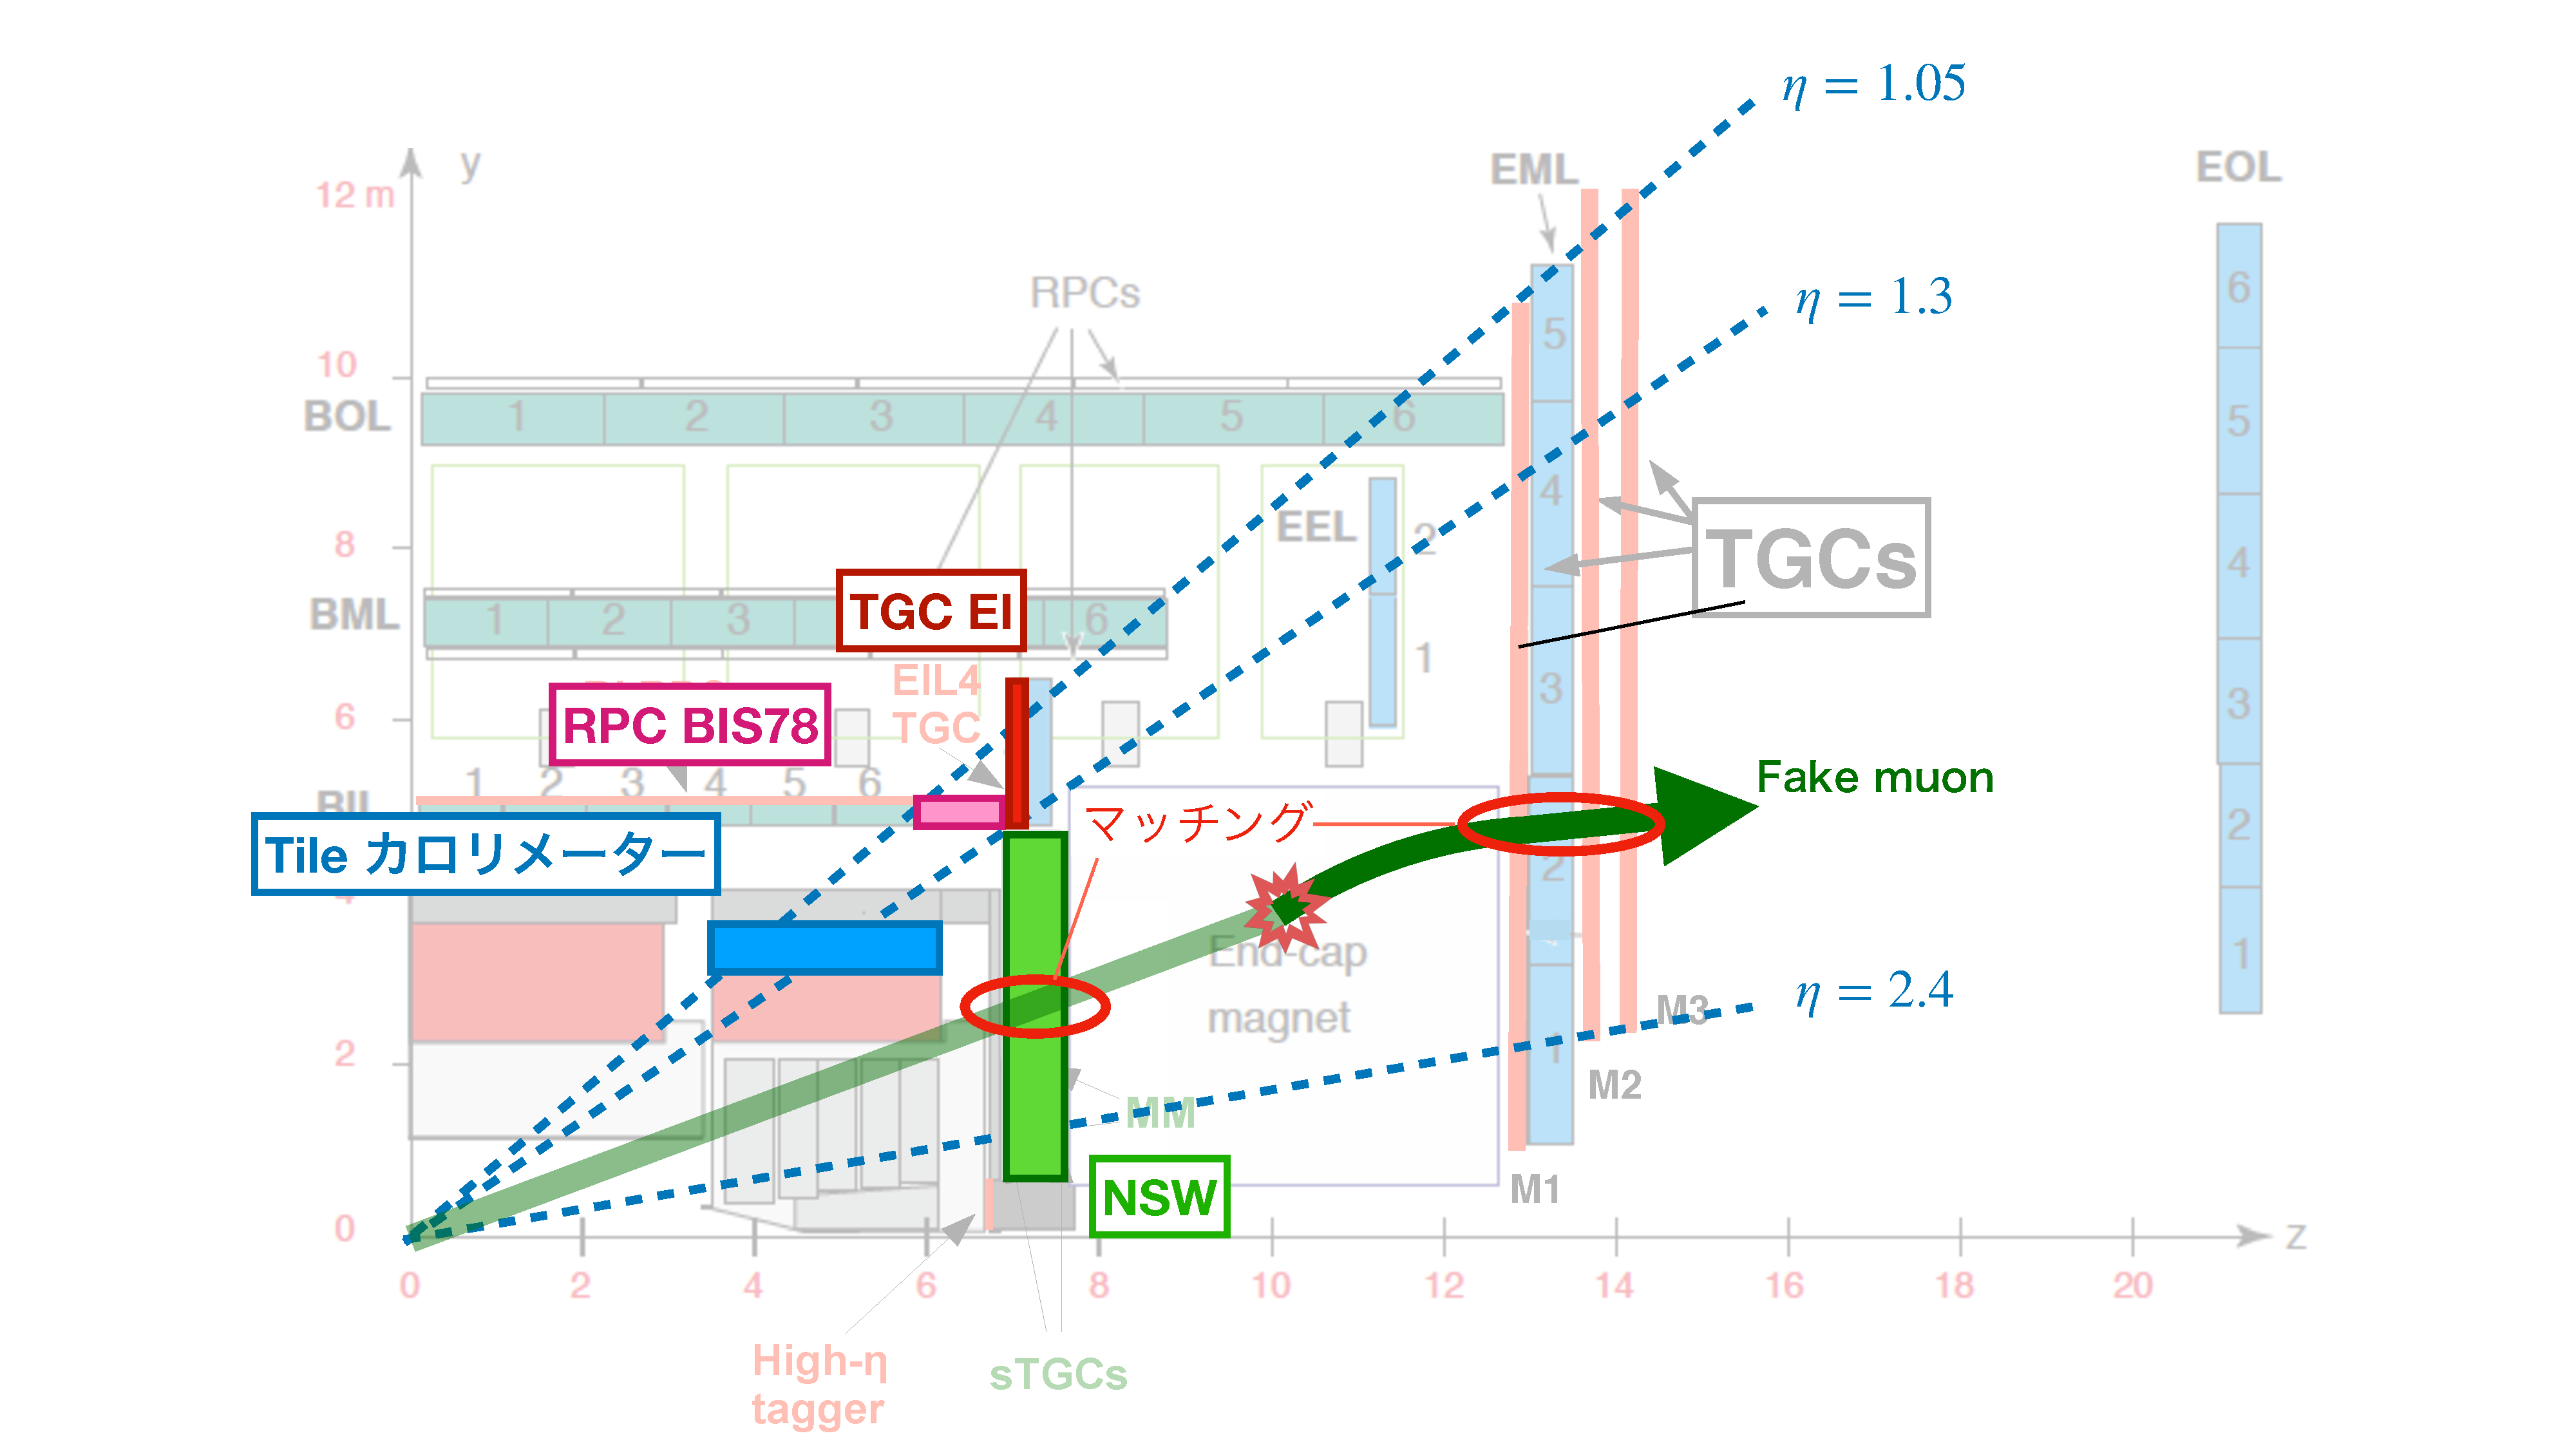
\includegraphics[width=16cm]{fig/Intro/TGC_Inner_concept.pdf}
    \caption[フェイクトリガーの例]{Inner Coincidenceの概念図\cite{mt_kawamoto}。エンドキャップトロイド磁場内部の検出器にヒットを要求することで、衝突点由来でない荷電粒子に対してトリガーを発行してしまう事象を削減する。}
    \label{TGC_Inner_concept}
\end{figure}

    \subsection{Run 3でのTGC検出器システム}

\begin{figure} 
\centering
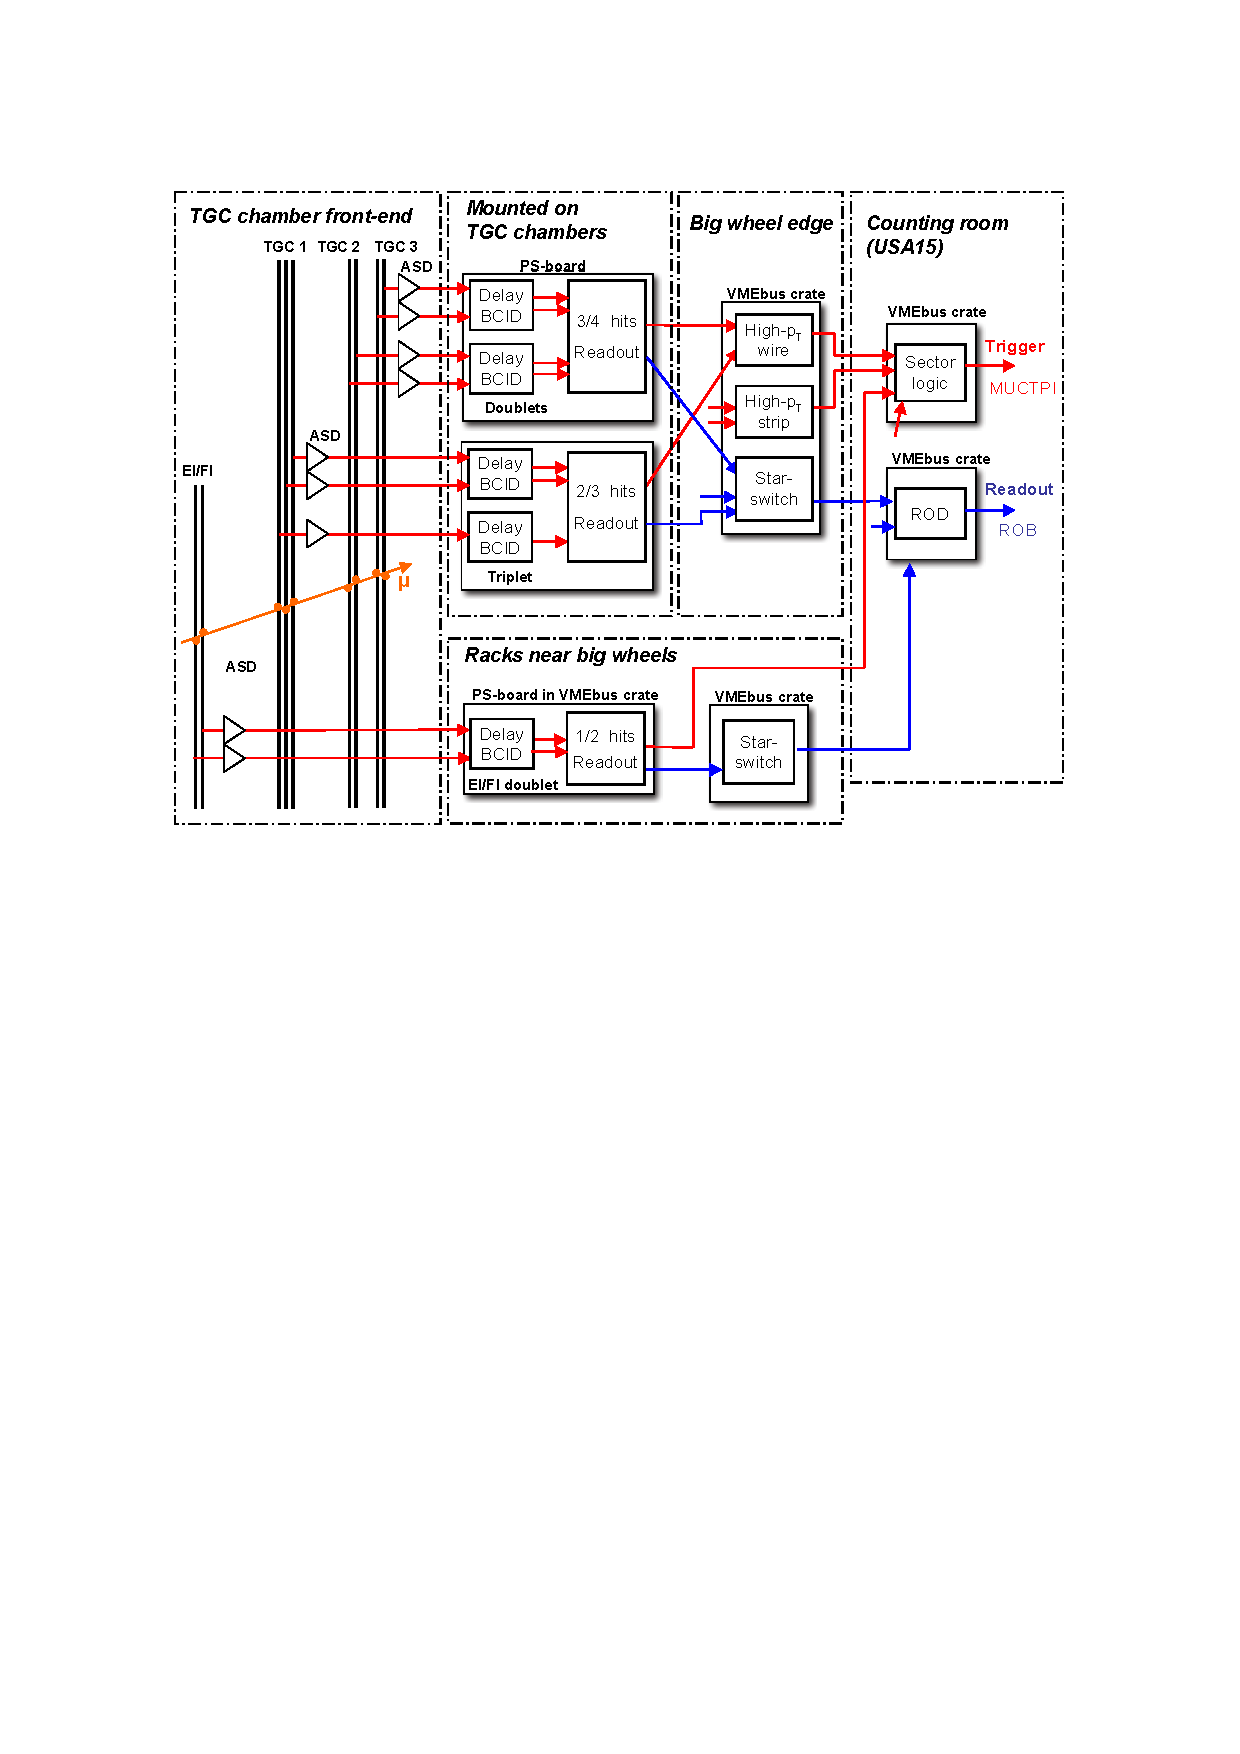
\includegraphics[width=16cm]{fig/Intro/TGC_run3tdaq.pdf}
\caption[Run 3におけるTGC TDAQシステム]{Run 3におけるTGC TDAQシステム。赤線がトリガーパス、青線が読み出しパスを表す。TGC検出器からの電流信号はASDでデジタル信号に変換され、PS boardに集められる。PS boardではBCIDが行われ、ワイヤーとストリップそれぞれでステーション内コインシデンスおよびM2-M3コインシデンスを取られる。その後HPTでM1-M3コインシデンスがとられたのち、SLでワイヤー・ストリップ間コインシデンス及び磁場内部に位置する検出器とのコインシデンスがとられる。SLで得られた$p_\mathrm{T}$情報はMUCTPIを介してCTPに送られ、L1 トリガー判定が行われる。L1 トリガー判定を待っている間、ヒットデータはPS board でバッファーされ、L1A信号が発行された場合にはSSW、RODを通して後段に読み出される。}
\label{TGC_run3tdaq}
\end{figure}

上記のトリガーコンセプトを実現する現行 (Run 3) のTGC TDAQシステムのブロック図を図\ref{TGC_run3tdaq}に示す。図の赤色の線はトリガー判定のための信号の流れを示しており、LHCの陽子バンチ交差に同期してFixed latencyで動作する (トリガーパスと呼ぶ)。青色の線はL1A後のデータ読み出しのための信号の流れを示しており、LHCとは非同期に動作する (読み出しパスと呼ぶ)。TGC検出器にミューオンが入射すると、ガスレイヤーに張られたワイヤーとストリップでアナログの電流信号が発生する。アナログ信号はTGC検出器に直接取り付けられたAmplifier Shaper-Discriminator  (ASD) に集められる。ASDは信号を電圧信号に変換し増幅した後、閾値電圧との比較によりデジタル信号を生成する。デジタル信号は後段のPS board上に搭載されたPatch-Panel ASIC  (PP ASIC) において、どの陽子バンチ交差に由来するものか識別される  (BCID) 。この後から信号はトリガーパスと読み出しパスに分けられる。

トリガーパスは、Slave Board (SLB) ASIC、High-pt (HPT)、Sector Logic (SL) で構成される。SLBではまずワイヤーとストリップ、それぞれでステーション内コインシデンスがとられる。またM2、M3の間のコインシデンスがとられ、 ($\mathrm{d}R_{23}$,$\mathrm{d\phi_{23}}$)が計算される。その後HPTでM1、M3間のコインシデンスがとられ、($\mathrm{d}R_{13}$,$\mathrm{d\phi_{13}}$)が計算さる。SLではM3におけるヒット位置および ($\mathrm{d}R_{13}$,$\mathrm{d\phi_{13}}$)をもとにワイヤー・ストリップ間のコインシデンスがとられ、\pt が概算される。またInner Coincidenceにより、背景事象の除去およびより精度の高い\pt 計算が行われる。SLで再構成された入射位置と\pt 情報は MUCTPI に送られ、CTPへ渡される。CTPでトリガー条件を満たしたバンチ交差にはL1Aが発行される。

読み出しパスはSLB、Star SWitch (SSW)、ReadOut Driver (ROD) というパスを経由して後段へ渡される。PP ASICで同期された信号は、トリガー判定が完了するまでSLB内のL1 Bufferに保存される。SLBでは最大128イベント分の信号をバッファリングすることが可能である。前節で述べた通り、L1 TriggerはFixed latency Schemeを採用しており、L1 Bufferにデータが入ってからそのイベントにL1Aが出されるまでの時間  (L1 latency) は固定されている。そのためSLBはL1Aを受信した後、L1 latencyだけ前のデータを読み出すことで、正しくデータを読み出すことができる。SLBから読み出されたデータはSSWでゼロサプレスと呼ばれるデータ圧縮が行われ、イベント毎にパッケージされる  (Event Building)。RODは1つのセクター内の全てのSLB-SSWから送られたデータ集約し、さらに後段のReadOut System  (ROS) へとデータを送信する。

これらのTGCエレクトロニクスのうち、ASD、PS board、HPT、SSWはATLAS実験室内に設置され、フロントエンドエレクトロニクスと呼ばれる。図\ref{TGC_elec_mount}にフロントエンドエレクトロニクスの設置場所を示す。ASDはTGCチェンバーに直接取り付けられたアダプタボードにマウントされる。PS boardは2枚ごとにアルミニウムで作られたケース  (PS-pack) に収納され、TGCチェンバー付近に設置される。HPTおよびSSWはBWの外側にあるMini-Rack内のVMEクレートに収められる。SL、ROD以降のエレクトロニクスはUX15からUSA15というATLAS回路室内に設置され、バックエンドエレクトロニクスと呼ばれる。HPTとSLおよびSSWとRODはRun 3ではG-linkと呼ばれる旧式の光シリアル通信規格で接続される。G-linkにおけるシリアルデータ転送レートはおよそ800 Mpbsである。

\begin{figure} 
    \centering
    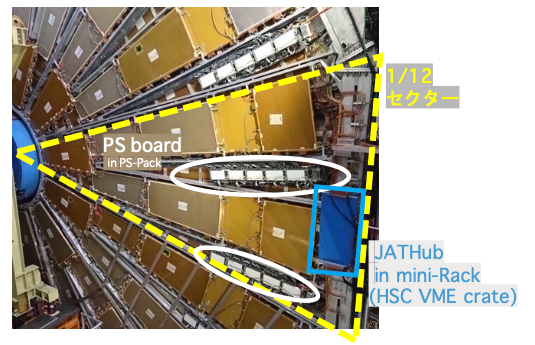
\includegraphics[width=16cm]{fig/Intro/TGC_elec_mount.pdf}
    \caption[TGCエレクトロニクスが設置されている場所]{TGCエレクトロニクスの設置場所。ASDはTGCチェンバーに直接取り付けられたアダプタボードに設置される。PS board は検出器付近のPS-packに収納される。HPT および SSW は BWの外側に設置されたMini-Rack内のVMEクレートに収められる。}
    \label{TGC_elec_mount}
\end{figure}

次にTTC系について述べる。Level1 Bufferより前の読み出し回路およびトリガー回路は、Fixed latency schemeを実現するためLHCの陽子バンチ交差と同期して動作する必要がある。この同期のために、各検出器とLHCを同期させるシステムをTiming, Trigger and Control  (TTC) システムとよび、そのために配布される信号をTTC信号と呼ぶ。TTC信号には陽子バンチ交差と同期した40.079 MHzのLHCバンチ交差クロック  (LHCクロック) やL1A信号などが含まれる。Run 3におけるTTC系の概要を図\ref{Run3_TTC}に示す。TTC信号はCTPから各検出器サブシステムのLocal Trigger Processor  (LTP) に配られる。その後TTC信号はTTCvi、TTCex、TTXrxと呼ばれるTTC専用モジュールおよび専用線を通じて、PS board、HPT、SSW、SLへ分配される。

\begin{figure} 
\centering
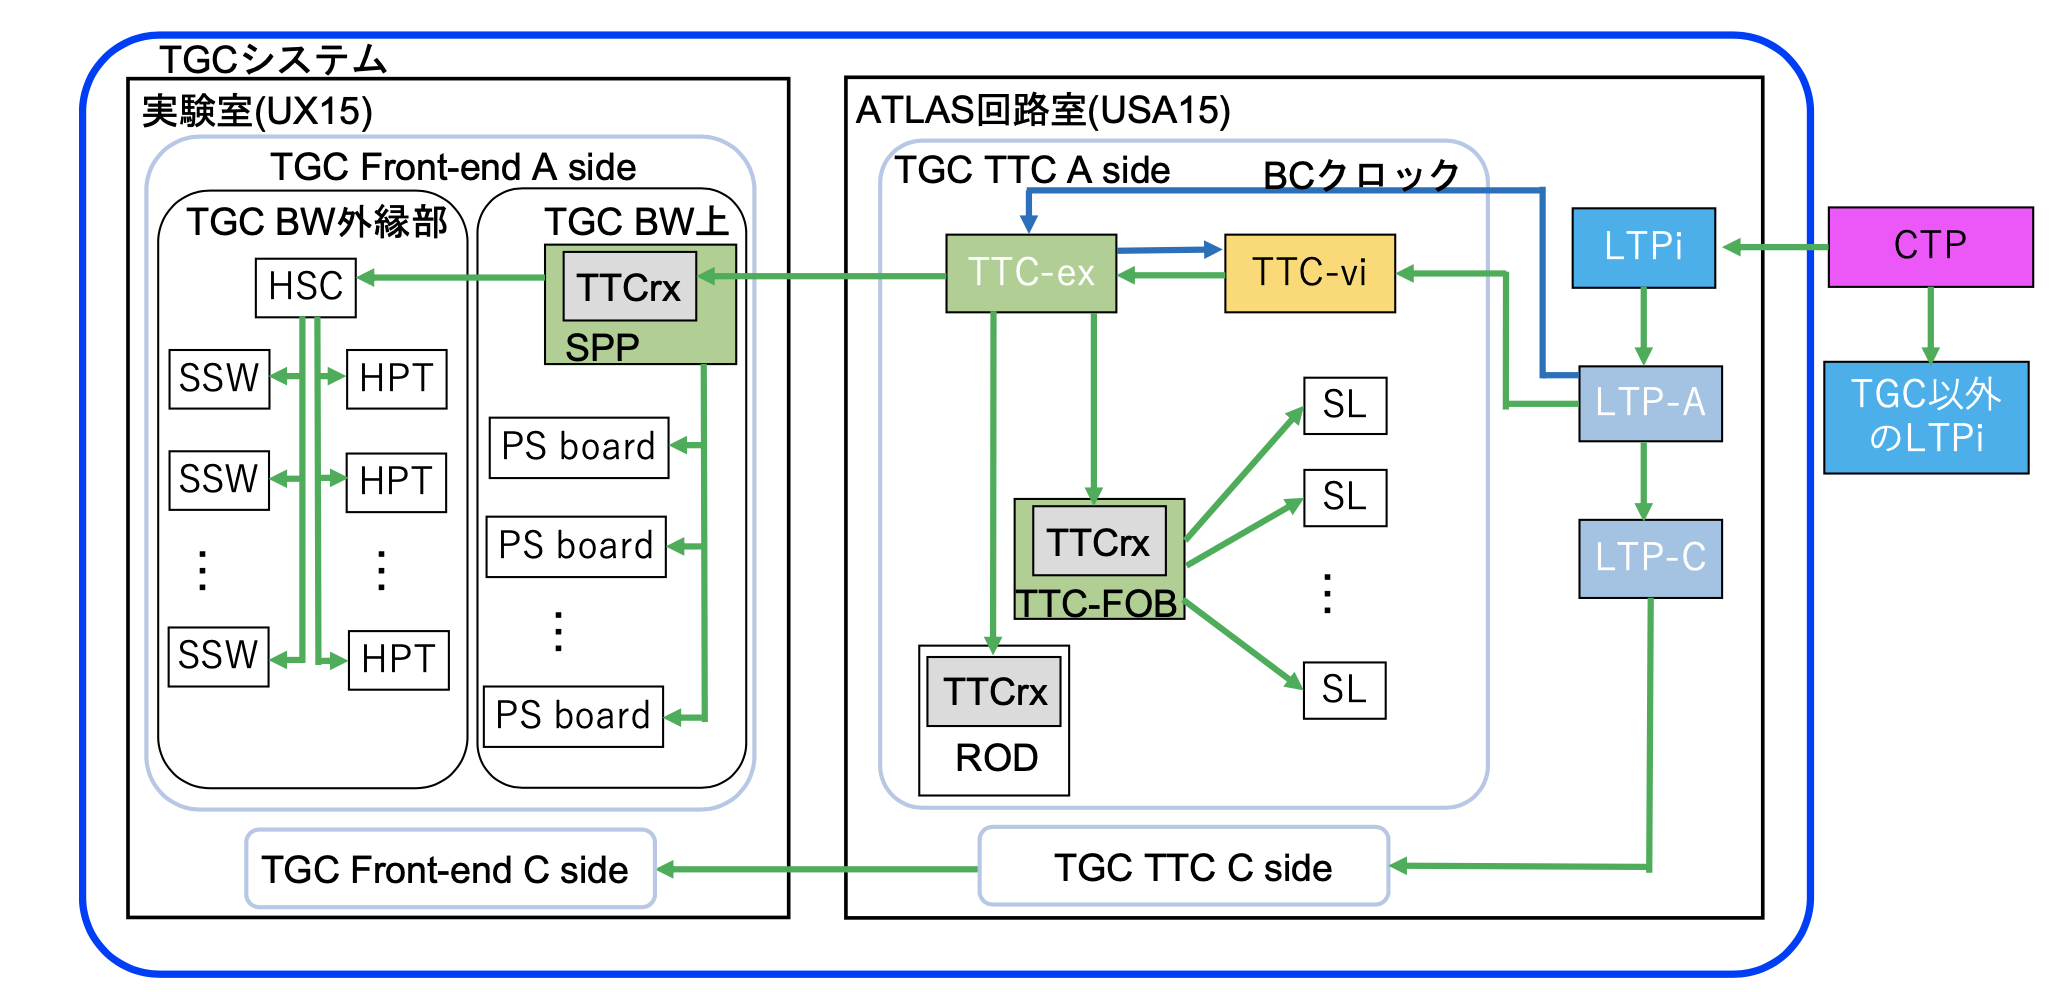
\includegraphics[width=16cm]{fig/Intro/Run3_TTC.png}
\caption[Run 3 TGCシステムにおけるTTCシステムの概要]{Run 3 TGCシステムにおけるTTCシステムの概要\cite{JINST:2008}。TTC信号はCTPから各検出器のサブシステムのLTPに分配され、TTCvi、TTCex、TTCrxを介してPS board、HPT、SSW、SLへと分配される。}
\label{Run3_TTC}
\end{figure}

以上に述べたRun 3のTDAQシステムでは、高輝度LHC-ATLAS実験のトリガーおよび読み出し性能の要求を満たすことができない。この限界は、主にSLBに設置されるL1 Bufferの容量と、ATLAS実験室と回路室間の帯域幅に由来している。Run 3では、L1 Bufferは最大128イベント分のデータしか保存できないため、高輝度LHC-ATLAS実験のL0 latencyの要求である10us  (400バンチ) の間データを保持することができない。さらに、1 MHzの初段トリガーレートに対応するデータ量を読み出すためには、現行システムのATLAS実験室と回路室間の帯域幅では不十分である。

    \subsection{高輝度LHC-ATLAS実験でのTGC検出器システム}  
前節で述べた問題を解決するため、高輝度LHC-ATLAS実験ではTGC検出器のエレクトロニクスを大幅にアップグレードする。主な変更点はPS boardでBCIDしたすべてのヒット信号を、ヒットの有無に関わらず、すべてのBCについてSLに送る点である。Run 3のトリガーパスでは、検出器からの信号はSLBやHPTでのコインシデンスを通じて、段階的にデータ量を削減しながら回路室へ送られた。高輝度LHC-ATLAS実験では実験室と回路室の間で、新しく高速シリアル通信技術を導入し、帯域幅を大幅に拡張する。これにより、PS boardが処理した全チャンネル分のヒットビットマップをすべて、回路室のSLへ送信することができる。回路室では、ボードサイズや放射線耐性に対する制約が少なく、SLには大規模なFPGAを搭載することができる。その結果、CTPからL0Aが発行されるまでデータを保管しておくL0 Bufferも余裕を持って実装することができ、10 usのL0 latencyに対応することが可能となる。またSLに1つのトリガーセクター内の全てのPS boardからのヒット信号を集約させることで、TGC BW 7層分のヒットデータを利用した、より包括的なトリガーアルゴリズムを実現する。高輝度LHC-ATLAS実験でのトリガーロジックの詳細は\ref{sec_Phase2TriggerLogic}節で説明する。

\subsection*{全体像}
図\ref{TGC_phase2tdaq}に高輝度LHC-ATLAS実験でのTGC検出器エレクトロニクスの概要を示す。ASDは現行システムのものを引き続き使用する。一方で、Run 3で使われていたPS board、SLB、HPT、SLはすべて撤去され、新しくPrimary ProceSsor board  (PS board)、JTAG AssisTance Hub  (JATHub)、Endcap Sector Logic  (SL) が設置される。PS boardはRun 3と同様にPS-packに格納され、TGC検出器付近に設置される。JATHubはMini-pack内のVMEクレートに設置される。SLはUSA15のATCAクレートに設置される。1つのSLはTGCの1/24セクター担当し、このセクターを担当する最大31枚のPS boardからヒットデータを受け取る。

\begin{figure} 
\centering
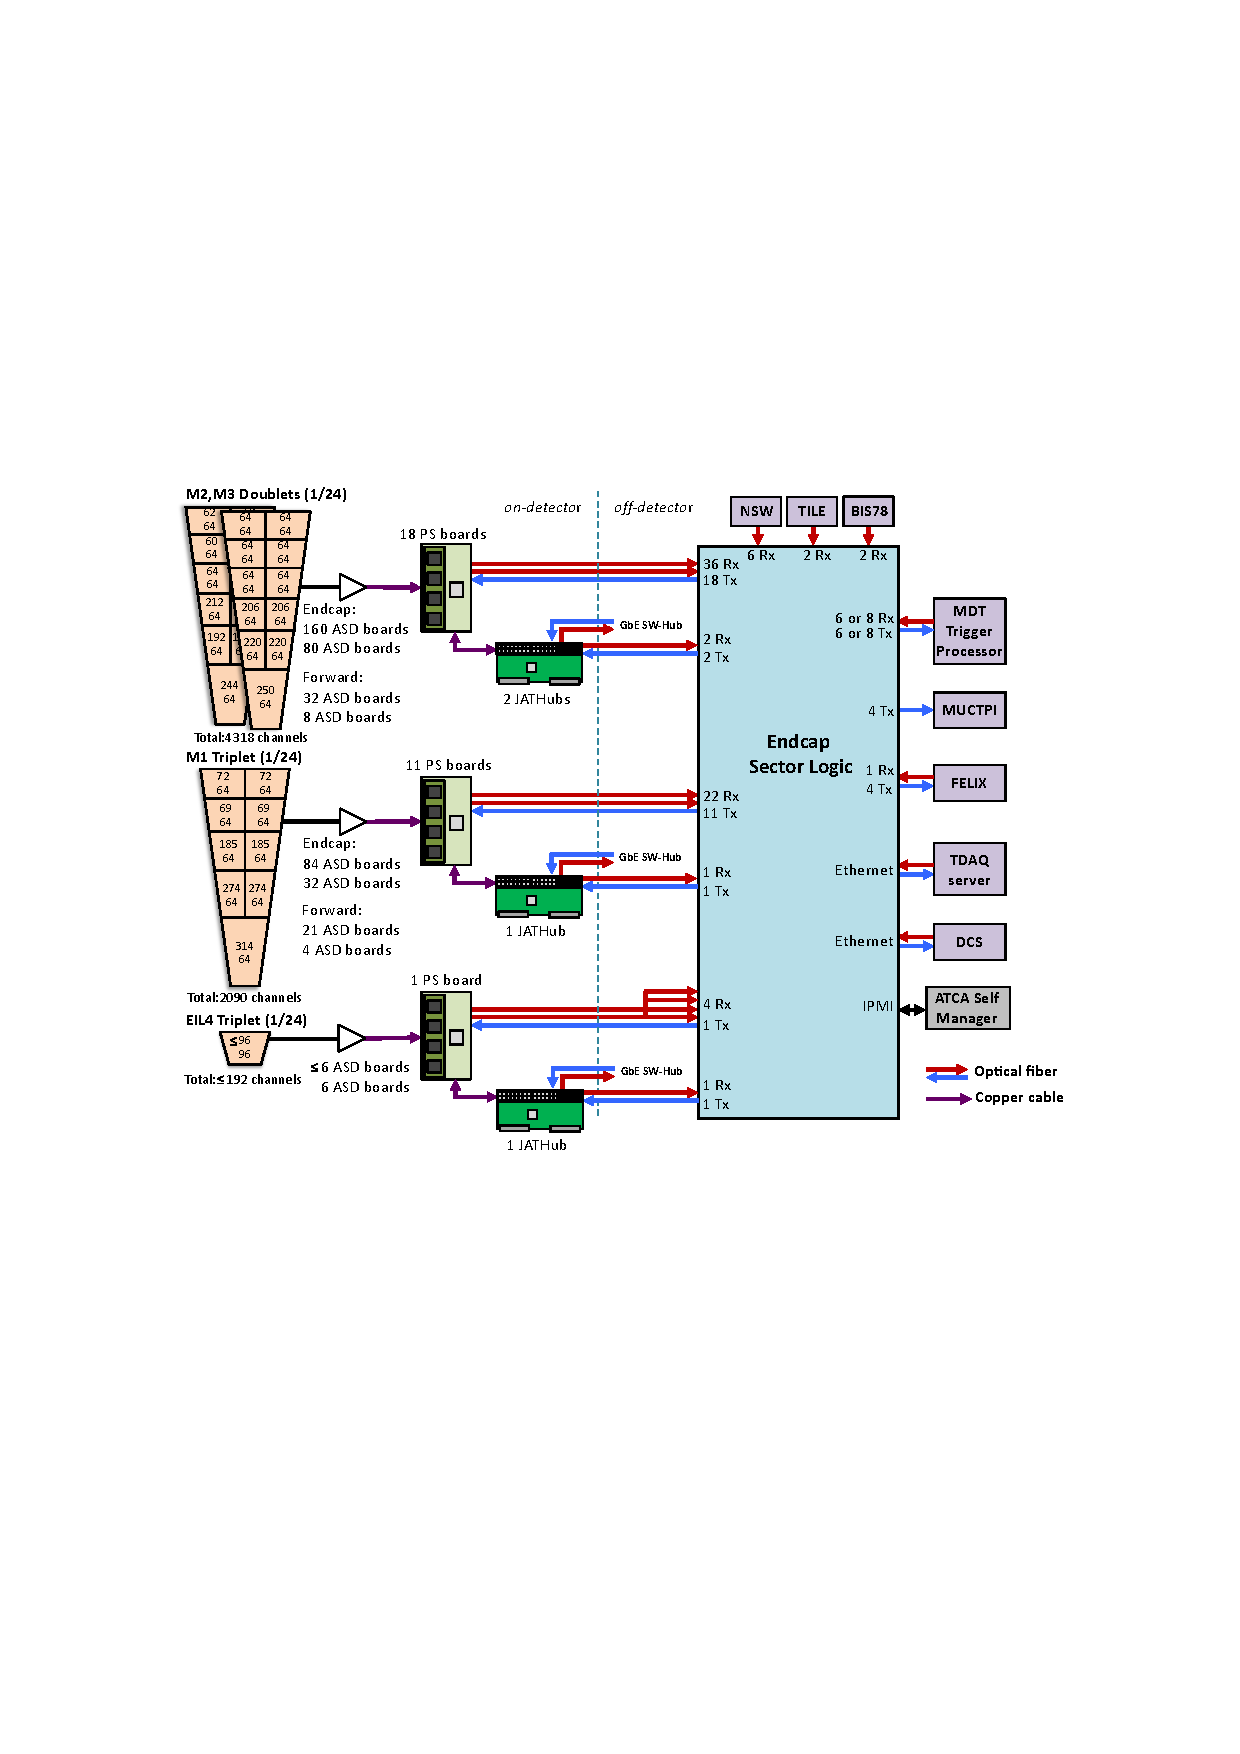
\includegraphics[width=16cm]{fig/Intro/TGC_phase2tdaq.pdf}
\caption[高輝度LHC-ATLAS実験におけるTGC検出器システムの概要]{高輝度LHC-ATLAS実験におけるTGC検出器システムの概要\cite{tdr_phase2muon_2017017}。TGCからの電流信号はASDでデジタル信号に変換され、PS board上のPP ASI で BCIDされる。PP ASIからのヒット信号はヒットの有無に関わらず、PS board FPGA から光ファイバーを通じてSLへ送られる。1枚のSLは1つの1/24セクターを担当し、PS board からのヒット信号に加えてTGC EI、NSW、RPC BIS78、Tile カロリーメーターの情報も利用して$p_{\mathrm{T}}$を判定する。その後SLは再構成した飛跡情報をMDT Trigger Processorに送信し、より精度の高い$p_{\mathrm{T}}$を計算する。SLからのトリガー出力は、MUCTPIを介してCTPへ送信され、L0 トリガー判定が行われる。CTPでL0 トリガー判定を待っている間、衝突データはSLでバッファーされ、L0Aが出されたものはFELIXを通して後段へ読み出される。TTC信号はCTPからFELIXを介して各SLに分配され、PS board へのコントロール信号に乗せられPS boardに分配される。JATHubはデータパスとは独立したモジュールで、PS board の制御を担当する。}
\label{TGC_phase2tdaq}
\end{figure}

トリガー回路および読み出し回路は主にSL上のFPGAに集約される。TGCで生じる電流信号はASDでデジタル信号に変換された後、PS board上のPP ASICでBCIDされる。PP ASICからのヒット信号は、PS board上のFPGAでまとめられ、光ファイバーを通じてSLに送信される。SLは、PS boardから送られるTGC BW 7層の情報に加え、TGC EI、NSW、RPC BIS78、Tile カロリメーターの情報も用いてミューオンの\pt を概算する。その後SLはMDT Trigger Processor (MDTTP) にミューオン飛跡候補を送信し、よりよい分解能で\pt を再構成する。SLのトリガー出力はMUCTPI通じてCTPへ送信され、L0 トリガー判定が行われる。CTPでのトリガー判定を待っている間、ヒットデータはSL内でバッファーされ、L0Aが発行されたバンチ交差事象のデータはFELIXを通じて後段へ読み出される。

TTC信号はCTPからFELIXを通じて各SLに分配され、PS board へのコントロール信号に乗せて各PS board に分配される。JATHubはデータパスと独立しており、PS board の制御を担当する。
このシステムではバックエンドのSLとフロントエンドのPS boardが光リンクのみで接続されており、トリガー、データ読み出し、コントロール、TTCの分配をコンパクトに実現している。

以下にTGC検出器における読み出し、トリガー、制御に関わるういお0それぞれのエレクトロニクスとその役割を説明する。

        \subsection*{Amplifier-Shaper-Discriminator (ASD)}
    ワイヤー、ストリップからの電流信号はTGCのチェンバーに直接取り付けられた、Amplifier-Shaper-Discriminator  (ASD) ボードで電圧信号に変換された後に増幅され、閾値電圧との比較による信号識別を経て、最終的にLVDS規格のデジタル信号へ変換される。図\ref{TGC_ASD}にASDの概要を示す。ASDはチャージアンプである前段増幅器 (Preamplifier)、差動電圧増幅回路、コンパレーターから構成されている。前段増幅回路では、0.8 V/pCのゲインを用いて、16 nsの時定数で電流信号を電圧信号に変換する。その信号は差動電圧増幅回路で7倍に増幅され、コンパレーターで閾値電圧を超えている時間に対応するパルス長のLVDS信号に変換される。この閾値電圧はPS boardから設定できるようになっている。またASDにはTGCのチャージ出力をエミュレートするTest Pulse源が実装されており、ASD以降のトリガー・データパスの試験に利用される。1枚のASDボードには4枚のASDチップが搭載されており、1枚あたり4チャンネル、全部で16チャンネルの信号を処理する。TGCの読み出しチャンネルはおよそ32万チャンネルであるため、システム全体ではおよそ2万枚のASDボードが設置される。

    \begin{figure}
    \begin{minipage}[b]{.5\linewidth}
    \centering
    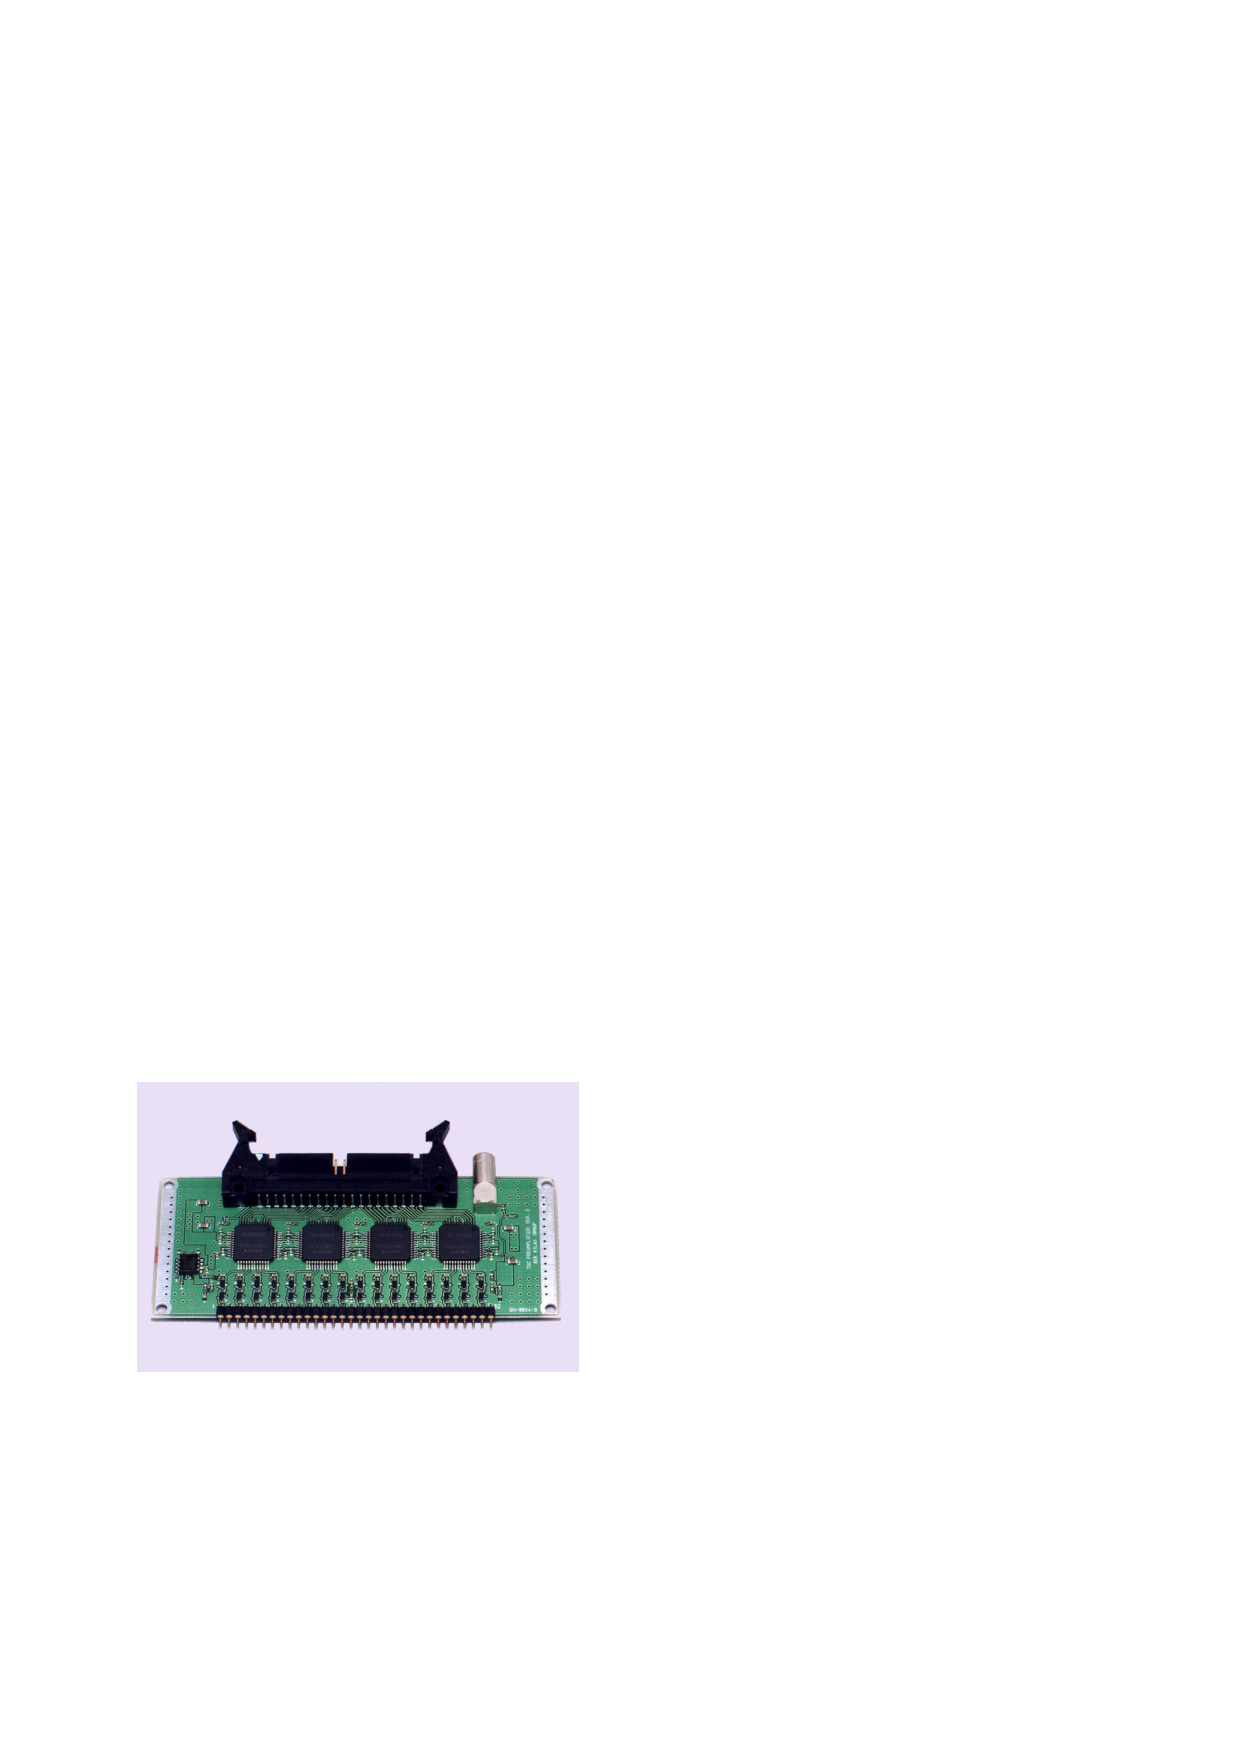
\includegraphics[height=5cm]{fig/Intro/TGC_ASD.pdf}
    \subcaption{ASDボードの写真}
    \end{minipage}%
    \begin{minipage}[b]{.5\linewidth}
    \centering
    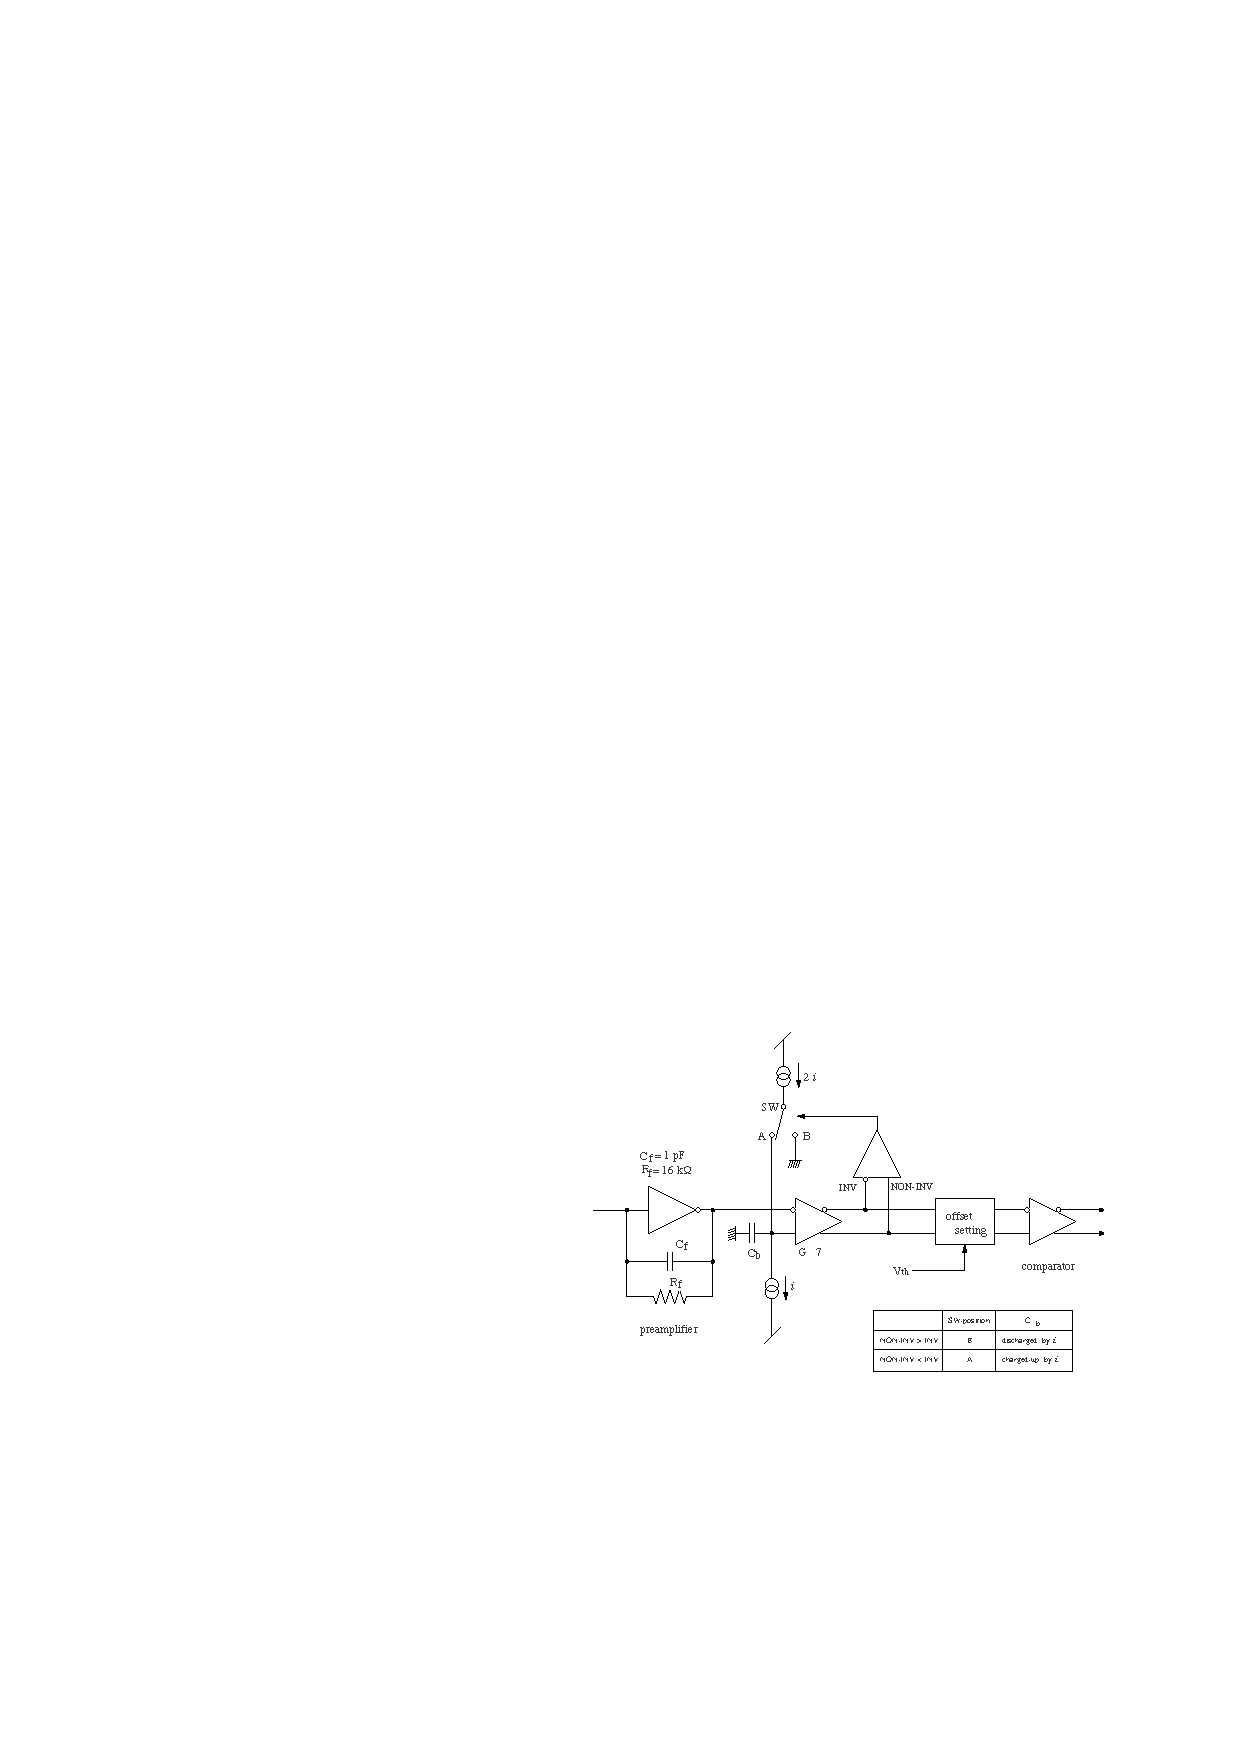
\includegraphics[height=5cm]{fig/Intro/TGC_ASDcircuite.pdf}
    \subcaption{ASDチップの回路ブロック図}
    \end{minipage}%
    \caption[ASDの概要]{ASDの概要\cite{ASD}。(a)にASDボードの写真を示す。1枚のASDボードには4枚のASDチップが搭載されており、1つにつき4チャンネル分のヒット信号を処理する。(b)にASDチップの回路図を示す。ASDチップは前段増幅回路、差動電圧増幅回路、コンパレーターから構成される。}
    \label{TGC_ASD}
    \end{figure}

        \subsection*{Primary ProceSsor board (PS board)}
    ASDボードからのヒット信号は、次にPS boardに送られる。PS boardはPP ASICとXilinx 社製のKintex-7 FPGAという2 種類の集積回路を搭載している。PP ASICは可変遅延機能により各ASDからの入力信号の到着時間を揃え、その信号がどの陽子バンチ交差に由来するかを識別する (BCID)。PS board FPGAはBCIDされたヒット信号を高速光シリアル通信に乗せてSLへ転送する。図\ref{TGC_PSB}にPS boardの最終試作機の写真とブロック図を示す。PS boardには8つのPP ASIが搭載され、そのうち4つはメザニンカードに乗せられる。1つのPP ASICは2台のASDと接続され、合計で32チャンネルの信号を処理する。PS board FPGAは8つのPP ASICからのヒット信号をまとめて、合計256チャンネル分のヒットビットマップをSLに送る。

    PS boardはボード上にDAC  (Degital Analog Converter) 、ADC  (Analog Degital Converter) 、クロックジッタークリーナー、QSPIフラッシュメモリーなどの電子素子を搭載している。DACはASDのコンパレーターにアナログの閾値電圧を供給する。PS board FPGAから閾値電圧の大きさを設定することができる。ADCはDACから供給される閾値電圧をモニターする。クロックジッタークリーナーは、PS board FPGAがシリアルデータから再構成したLHCバンチ交差クロックのジッターを低減する。QSPI フラッシュメモリーは不揮発性のメモリーで、ボードの電源が落とされた場合でも書き込まれた値を保持することができる。これを利用して、PS board FPGAのファームウェアや、ボードごとに最適化されたPP ASICの遅延値などのパラメーターを保存する役割を果たす。また、インターフェイスとして、電気信号を光信号に変換するSFP+モジュール、Cat-6ケーブルのコネクターであるRJ45を有しており、それぞれSLとJATHubに接続される。
    
    PS board はTGCシステム全体で1434 枚設置され、それぞれの個体の量産が2024 年から始まる。本研究では、量産される各個体にハードウェアの不具合がないことを検証する、品質保証試験の設計およびそれに向けた機能開発を行なった。これに関する詳細は\ref{chap_QAQC}章で議論する。
    以下にPP ASICとPS board FPGAの役割について詳しく説明する。

    \begin{figure}
    \begin{minipage}[b]{.5\linewidth}
    \centering
    \includegraphics[height=8cm]{fig/Intro/TGC_PSB.pdf}
    \subcaption{PS boardの写真}
    \end{minipage}%
    \begin{minipage}[b]{.5\linewidth}
    \centering
    \includegraphics[height=8cm]{fig/Intro/TGC_PSBblock.pdf}
    \subcaption{PS boardのブロック図}
    \end{minipage}%
    \caption[PS boardの概要]{PS boardの概要。1枚のPS board は、1つのFPGAと8つの PP ASIC (メインボードに4個、メザニンボードに4個)を搭載している。1つのPP ASICは2台のASDと接続され、合計で32チャンネルの信号を処理する。また、PS board はDAC、ADC、クロックジッタークリーナー、QSPIフラッシュメモリーなどの素子を搭載しており、これらはPS board FPGAからコンフィギュレーションすることができる。}
    \label{TGC_PSB}
    \end{figure}

    \subsubsection*{Patch-Panel ASIC (PP ASIC)}


    \begin{figure} 
    \centering
    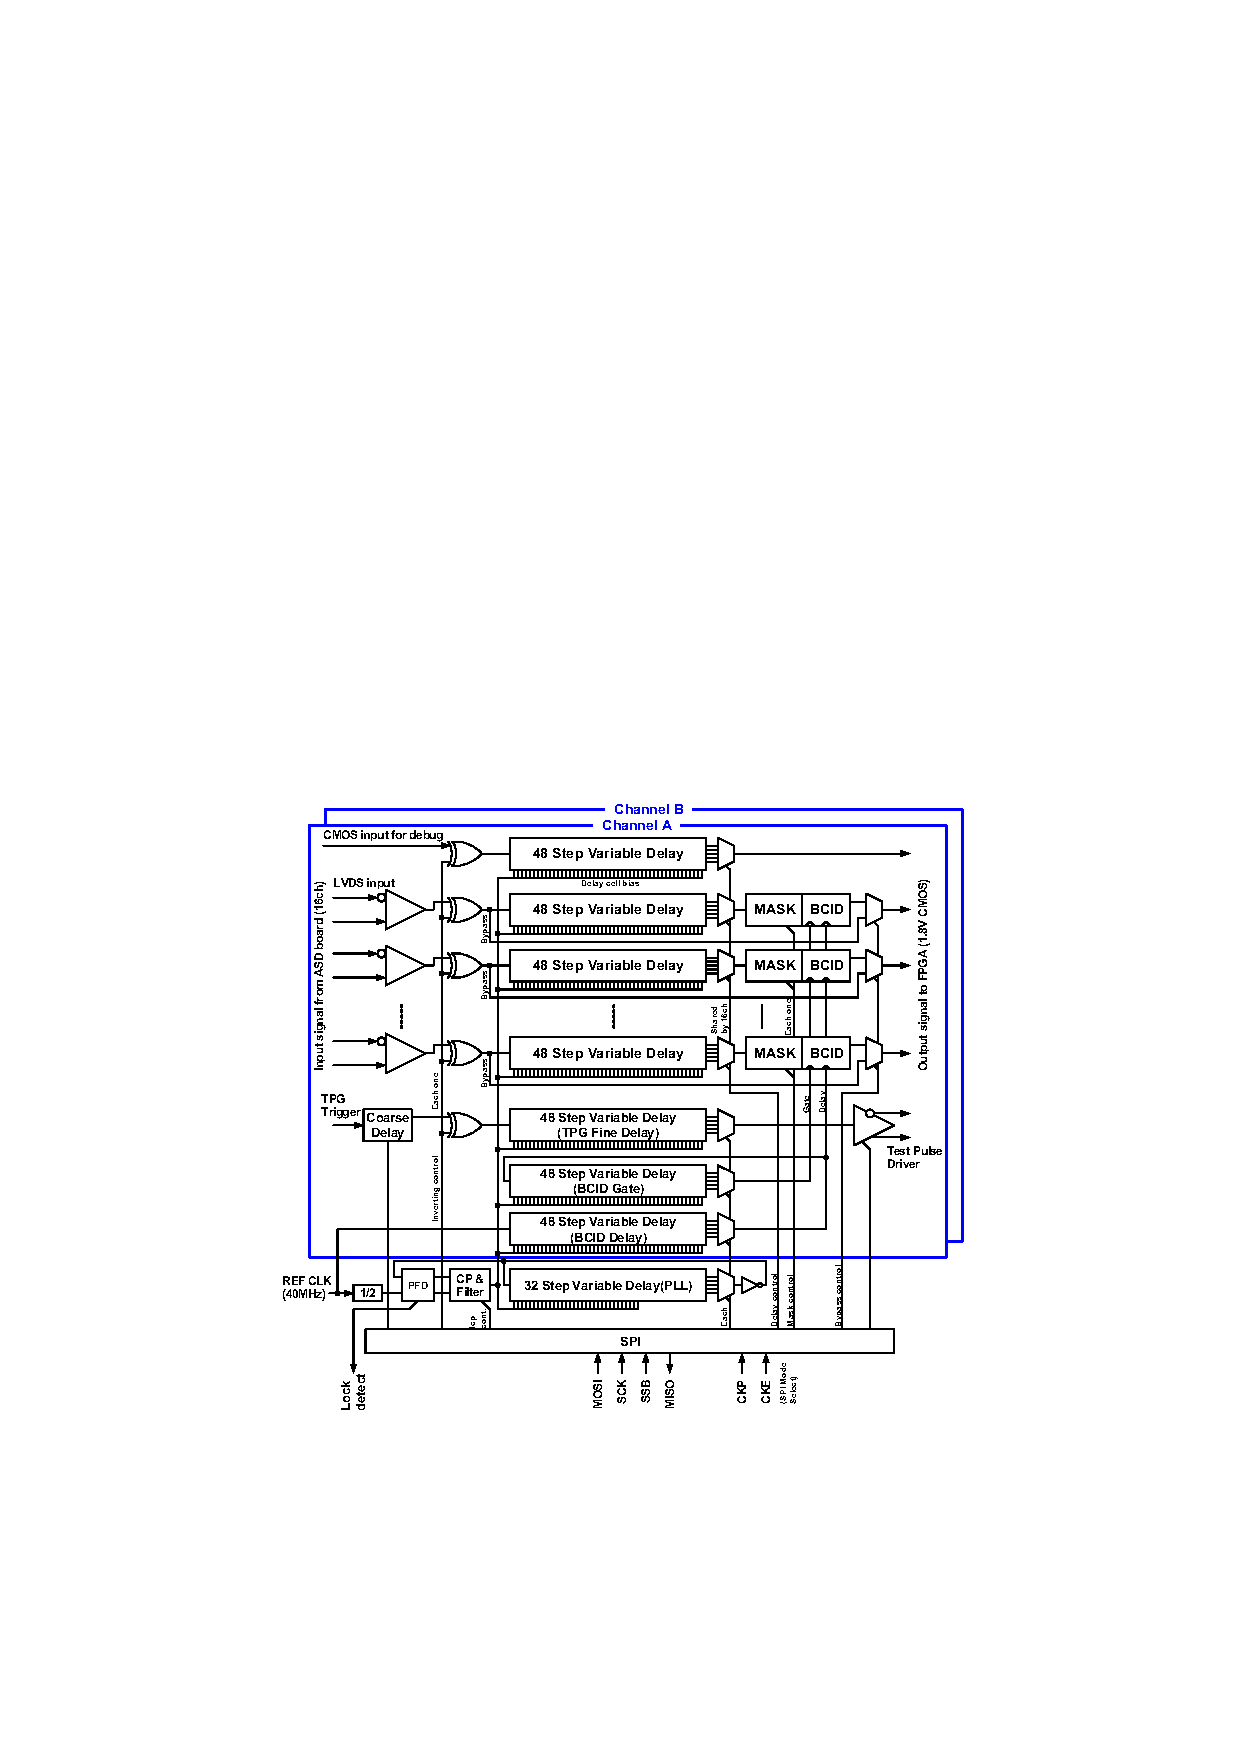
\includegraphics[width=16cm]{fig/Intro/TGC_PPASIC.pdf}
    \caption[PP ASIC回路のブロック図]{PP ASIC回路のブロック図\cite{PPASIC}。Channel AとChannel Bがそれぞれ1つのASDボードに対応し、1つの PP ASICは32チャンネルのLVDS信号を受け取る。PP ASICは主に可変遅延回路と陽子バンチ識別回路で構成され、この2つを用いてBCIDを行う。}
    \label{TGC_PPASIC}
    \end{figure}

    図\ref{TGC_PPASIC}にPP ASICのブロック図を示す。PP ASICは主に可変遅延回路と陽子バンチ識別回路で構成される。PP ASICが受け取るLVDS信号の入力時間には、チャンネルごとに$\mathcal{O}(10\,\mathrm{ns})$のばらつきが存在する。これは、衝突点から検出器までの飛行時間 (Time-of-Flight) や、ASDからPP ASICまでのLVDSケーブルの長さがチャンネルごとに異なるためである。また、同一チャンネル内でもイベントごとに信号の到着時間が20 $\sim$ 30 ns 程度変動する (図\ref{TGC_fructuation})。これは、ミューオンの入射位置に応じて、電荷が検出される位置からASDまでの距離が異なり、結果として信号の伝播遅延や電荷のドリフト時間にばらつきが生じるためである。

    \begin{figure} 
    \centering
    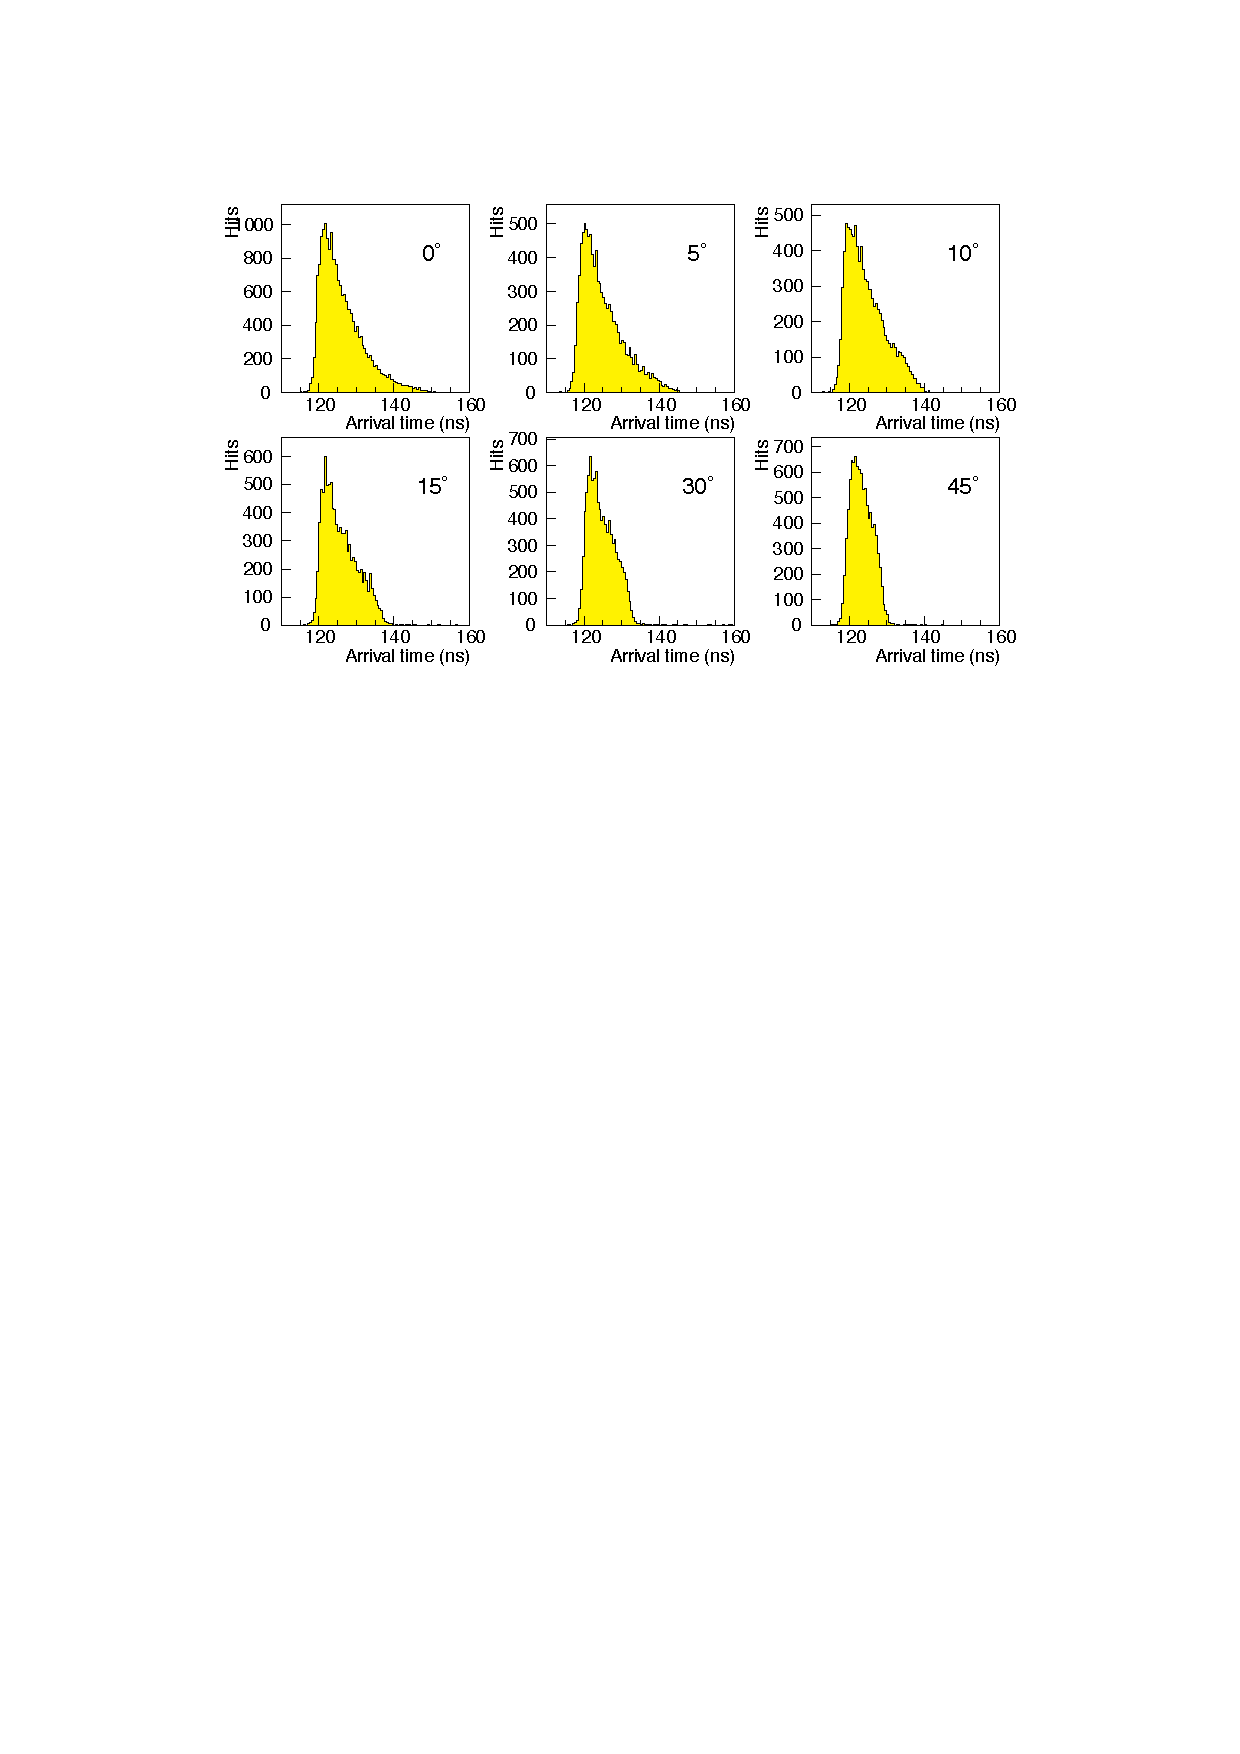
\includegraphics[width=16cm]{fig/Intro/TGC_fructuation.pdf}
    \caption[ミューオンがTGC検出器に入射してから、ASDに信号が到着するまでの時間分布]{ミューオンがTGC検出器に入射してから、ASDに信号が到着するまでの時間分布\cite{TGC_fructuation}。時間分布はミューオンが入射する角度に依存して、20 $\sim$ 30 nsの幅を持つ。}
    \label{TGC_fructuation}
    \end{figure}

    このばらつきを揃えるために、各ASDごとに固有の遅延を加えるのが可変遅延回路である。可変遅延回路は1 ns以下の刻み幅で、最大45 nsまでの遅延をかけることができる。PP ASICに一番遅く到着するASDからの信号の立ち上がりに、他のASDからの信号の立ち上がりを合わせるように遅延パラメーターが設定される。この遅延パラメーターはPS boardのFGPAから設定可能である。

    可変遅延回路でタイミングが揃えられた後、信号は陽子バンチ識別回路に送られる。陽子バンチ識別回路は、PP ASICに入射するデジタル信号の立ち上がりを検出し、その信号がどの陽子バンチ交差に由来するのか識別する。陽子バンチ回路の概念図を図\ref{TGC_BCID}に示す。前述の通り、同じチャンネル内であってもヒット信号の到着時間はイベント毎に20 $\sim$ 30 ns程度の幅を持ち、この時間幅のうちに来るヒット信号には同じBCIDを付与する必要がある。そのため、同じBCIDを付与する時間幅 (有効ゲート幅) をASDごとに設定できるようになっており、信号到着時間幅が25 nsを超える場合に対応するため、有効ゲート幅は25 ns以上に設定できるようになっている。その場合、2つの有効ゲートが重なる時間が存在するが、このタイミングに入射した信号には2バンチ分の信号が出力される。有効ゲート幅もPS boardのFPGAから設定することができる。

    \begin{figure} 
    \centering
    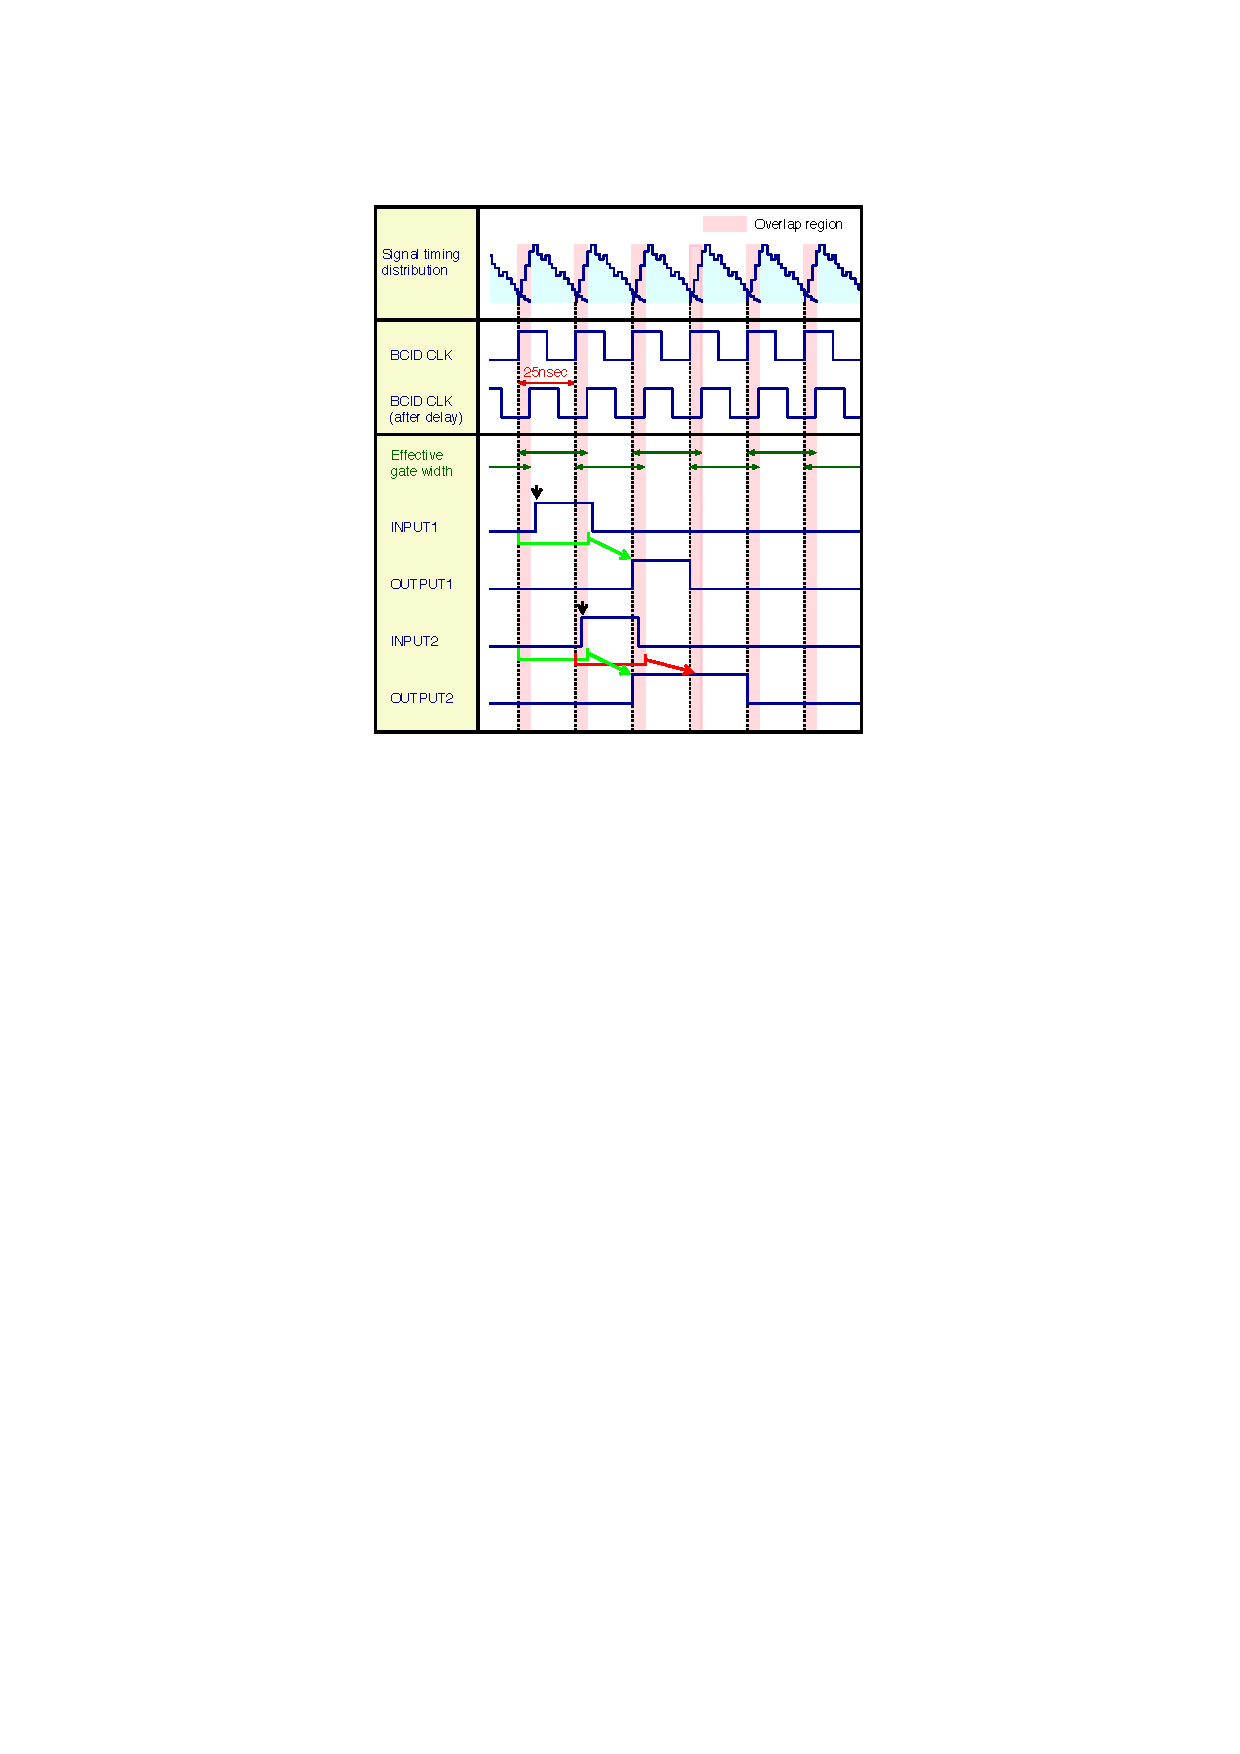
\includegraphics[width=14cm]{fig/Intro/TGC_BCID.pdf}
    \caption[陽子バンチ識別回路のタイミングチャート]{陽子バンチ識別回路のタイミングチャート\cite{mt_takemoto}。BCID CLKの立ち上がりのタイミングでINPUTがhighであった時、次のBCID CLKから1 BC分デジタル信号が出力される(INPUT1のとき)。BCID CLKの立ち上がりのタイミングが有効ゲートが重なる領域に来た場合には、2 BC分のデジタル信号を出力する(INPUT2のとき)。}
    \label{TGC_BCID}
    \end{figure}

    \subsubsection*{PS board FPGA}

    PS board FPGAはSLにヒットデータを送信することに加えて、PS board上の各素子の制御/監視およびLHCバンチ交差クロックの再構成を担当する。
    PP ASICによりLHCバンチ交差クロックと同期された256チャンネルのヒット信号は、PS board FPGAでまとめられ、光ファイバーを通じてSLに転送される。
    PS boardからSLに送信されるデータフォーマットを図\ref{TGC_PSBuplink}に示す。256チャンネルのヒットデータに加え、64 bitのヘッダーが付与され合計320 bitのデータが25 nsおきに送信される。320 bitのデータは2本の光ファイバーに分けられ、32 bitごとにワードとしてまとめられて送信される。ここでワード0ではヘッダーが、ワード1 $\sim$ 4にはヒットデータが詰められる。データ転送は高速シリアル通信で行われ、FPGA内のパラレルデータをシリアルデータに変換する際には8b10bコーディングが用いられる。そのため、1本の光ファイバーのラインレートは$160 \, \mathrm{bit} \times 10/8 \times 40 \mathrm{\,MHz} = 8 \,\mathrm{Gbps}$となる。

    \begin{figure} 
    \centering
    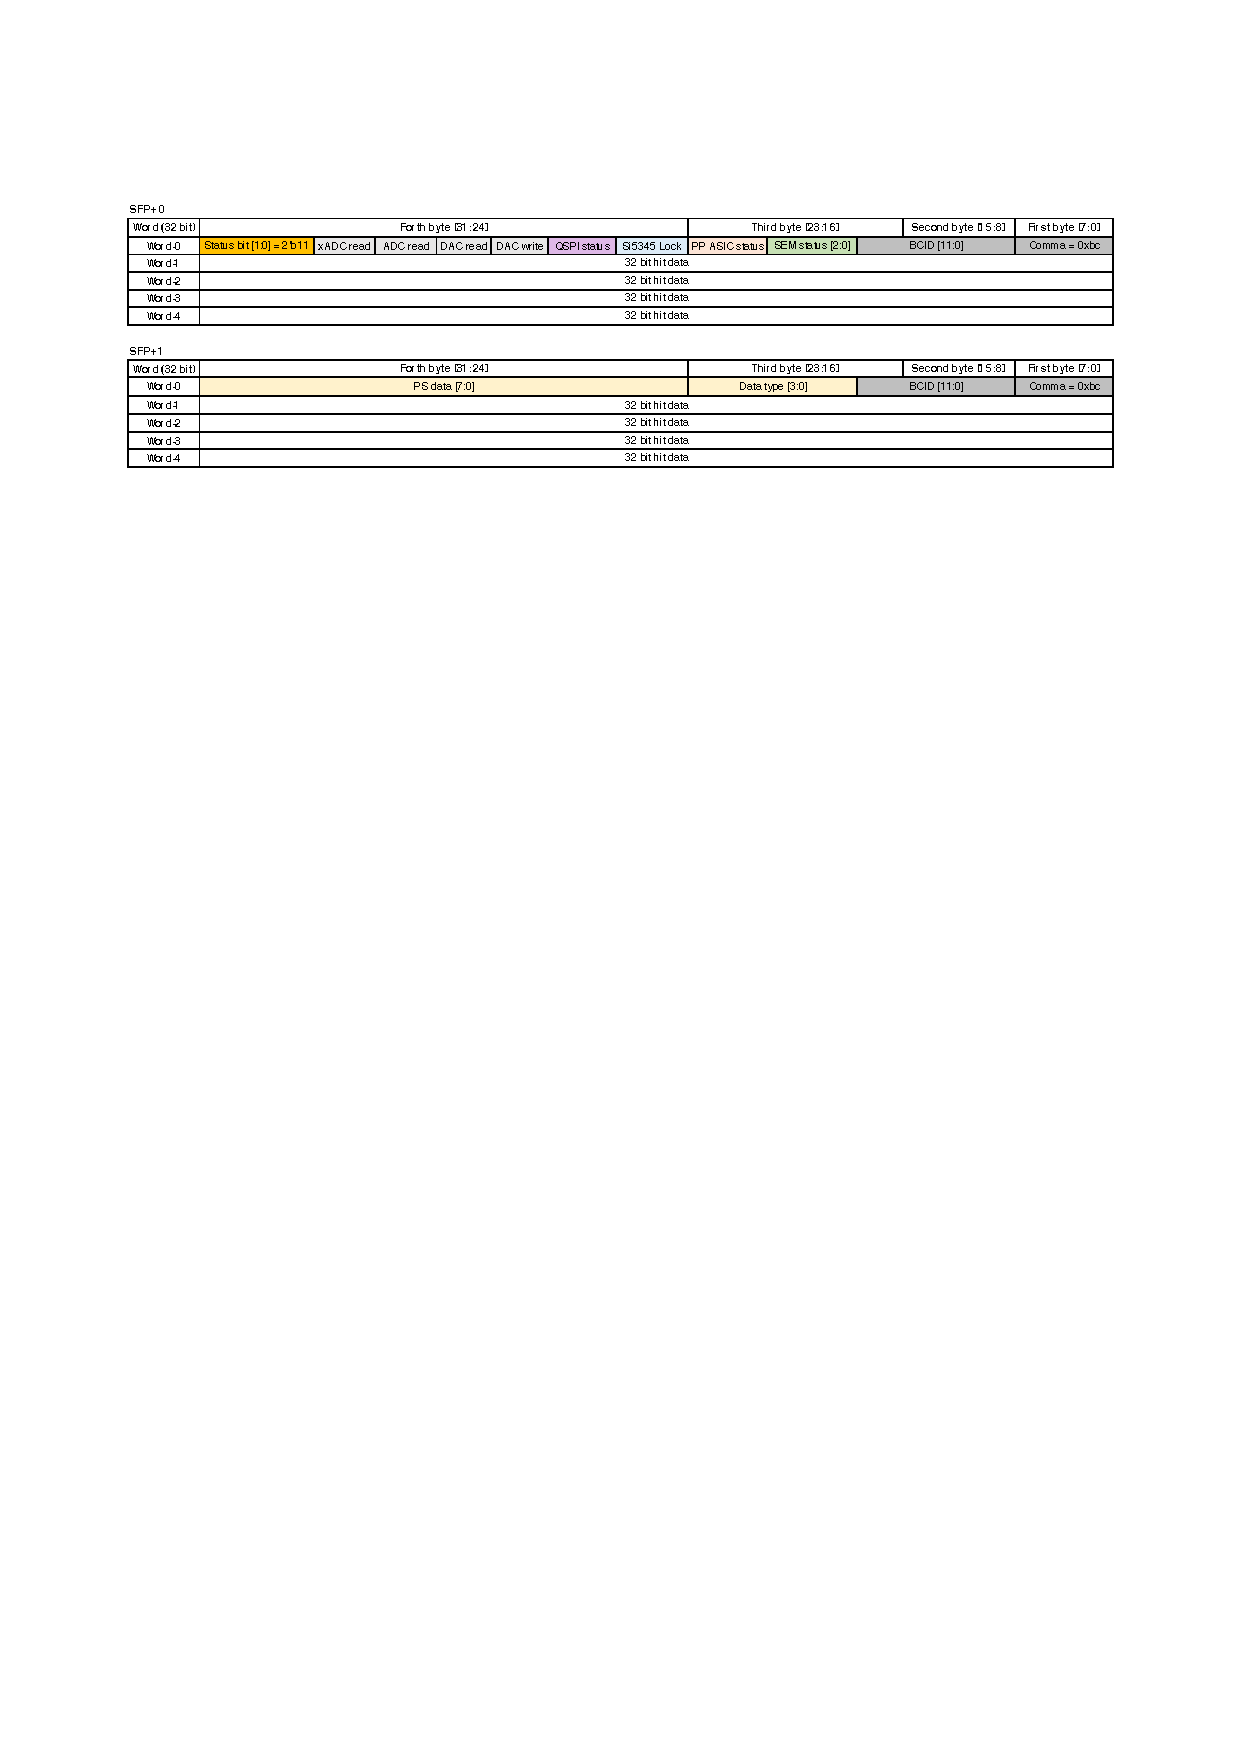
\includegraphics[width=16cm]{fig/Intro/TGC_PSBuplink.pdf}
    \caption[PS boardからSLへ送るデータフォーマット]{PS boardからSLへ送るデータフォーマット\cite{mt_aoki}。256チャンネルのヒットデータに64 bitのヘッダーが付与された、合計320 bit のデータが2リンクに分けられ、25 nsおきに送信される。ヘッダーワードには主にPS board FPGAやその他の素子のstatusを表すデータが含まれる。}
    \label{TGC_PSBuplink}
    \end{figure}

    PS board FGPAはSLからのコントロール信号を1本の光ファイバーを通じて受け取る。コントロール信号のデータフォーマットを図\ref{TGC_PSBdownlink}に示す。SLはワード2と3で定義されたAddress、Data、Commandを利用してPS board FPGA内のレジスタを操作する。PS board FPGAとQSPIフラッシュメモリーはSPIバスで接続されており、SLがFPGAを介してSPIバスを制御することで、QSPIフラッシュメモリーにデータを書き込むことができる。この通信パスを利用して、PP ASICの遅延パラメーターや有効ゲート幅、ASDに供給する閾値電圧などの制御用パラメーターをQSPI フラッシュメモリー上に保存することができる。

    PS board FPGAはQSPIフラッシュメモリーに保存された制御用パラメーターを読み取り、PP ASIC、ASDに自動で分配する。これを自立型制御機構と呼ぶ。この機構により、1434 枚のPS boardには同じファームウェア\footnote{正確にはPS boardからSLに送るデータフォーマットに3種類のバラエティが必要であるため、3種類のファームウェアを使い分けることになる。}を書き込んだ上で、ボード毎に必要な設定は自動で行うという、次世代的な制御モデルを実現している。
    PS board FPGA にはPS board上の素子の状態を監視するための機構も備わっており、DACに分配した設定値、ADC、xADC\footnote{Xilinx Analog-Digital Converter、FPGA内部の温度、電源電圧、外部からのアナログ信号を監視するためのモジュール。PS boardに供給される3.3 VD  (デジタル) 、+ 3 VA  (アナログ) 、-3 VAをモニターする}のモニター値、GTXトランシーバーのロック信号を定期的に読み出し、SLに送信する。これによりSLはフロントエンドのPS boardの状態を常に把握し、異常が生じた際には瞬時に対応することができる。

    \begin{figure} 
        \centering
        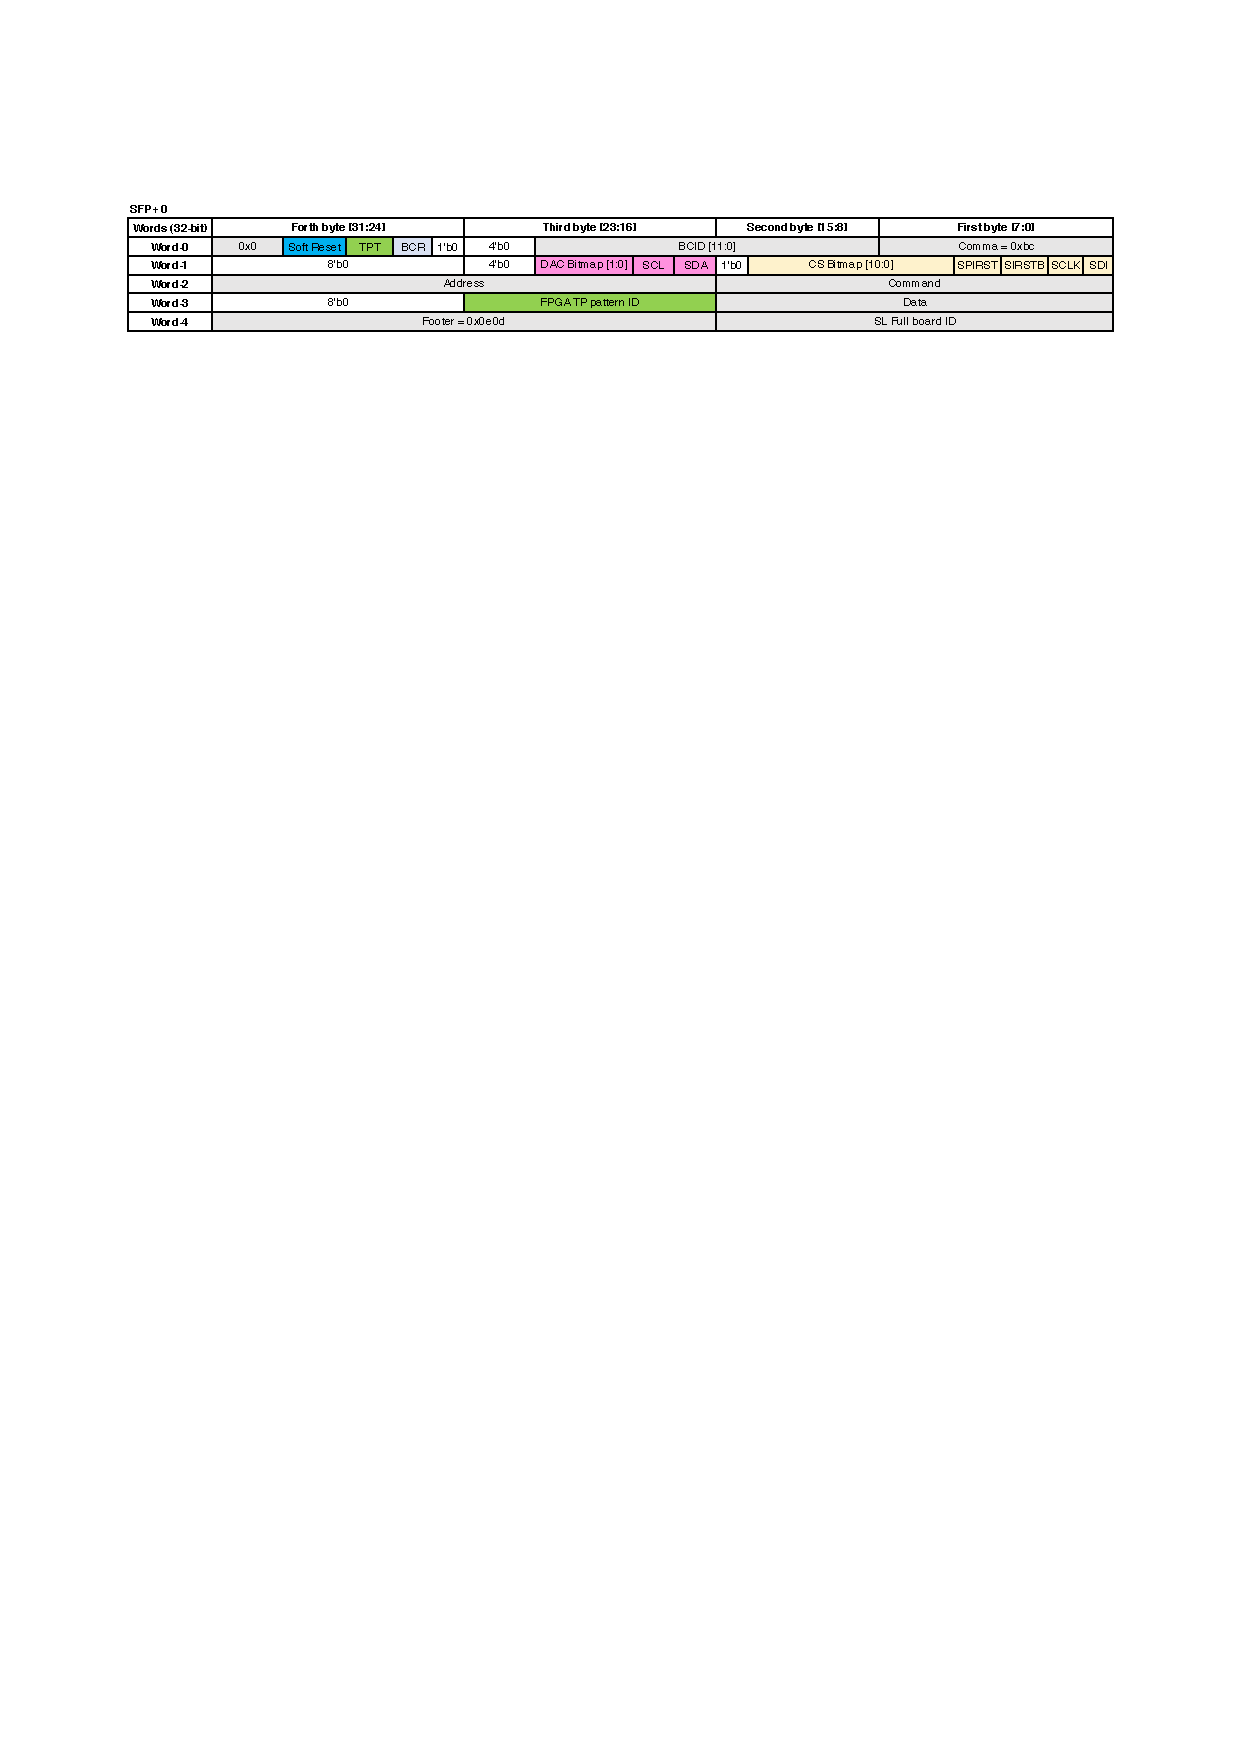
\includegraphics[width=16cm]{fig/Intro/TGC_PSBdownlink.pdf}
        \caption[SLからPS boardへ送るコントロールデータのフォーマット]{SLからPS boardへ送るコントロールデータのフォーマット\cite{mt_aoki}。Word0にはTTC信号、Word1にはビットバンギング用のデータ、Word 2、Word3にはPS board FPGA内のレジスタ操作用のデータが含まれる。}
        \label{TGC_PSBdownlink}
    \end{figure}
    
    TTC信号もこのコントロール信号に乗せられてPS boardに分配される。PS boardのGTXトランシーバーは、ワード0で定義されるComma ワードを使用して、シリアルデータからLHCバンチ交差クロックを再構成する。PS boardで再構成されたLHCバンチ交差クロックはPS board 間で位相を揃えるための適切な遅延が加えられた後、ジッタークリーナーを経由してFPGA、GTXトランシーバー、PP ASICへ分配される。    

    さらに、PS boardは放射線損傷に対する堅牢性を実現するシステムを搭載している。PS boardは実験室に置かれるため、FPGAは電子回路上のメモリのビットが反転してしまうSingle Event Upset (SEU) などの放射線損傷を受ける可能性がある。先行研究\cite{PSB_SEU}によると、1つのPS board FPGAでは3時間に一回程度SEUが発生する。FPGAには修復可能なSEU  (1ビットエラーおよび隣接する2ビットエラー)を自動的に修復するSoft Error Mitigation Controller  (SEM) が実装されている。また修復不可能なSEU  (隣接しない2ビットエラーおよび3ビット以上のエラー) が生じた際には、PS boardの制御を担当するJATHubに対して救難信号を送り、JATHubにFPGAの再コンフィギュレーション用の信号を送信させることでこれに対処する。このように、放射線損傷に対して堅牢なシステムを実現することで、データ取得時のデッドタイムを最小限に抑えることができる。    

        \subsection*{JTAG AssisTance Hub (JATHub)}
    JATHubはデータパスとは独立した、PS board制御用の回路である。概要を図\ref{TGC_JATHub}に示す。JATHubはXilinx社製のZynq-7000 SoCをメインドライバーとして搭載する。Zynqはプロセッサー部分であるProcessing System  (PS) と、FPGA部分であるProgrammable Logic  (PL) で構成されている。PS部分ではLinuxなどのカーネルを立ち上げることが可能で、C言語などで記述されたアプリケーションを実行してFPGAを操作することができる。これにより、JATHubは高い自由度と拡張性を実現する。
    JATHubはインターフェイスとして、PS boardとLVDS通信するためのRJ45コネクターと、イーサーネット通信のためのSFP+モジュールを搭載している。1枚のJATHubは最大で11枚のPS boardと接続可能であり、それぞれ2本のCat-6\footnote{Category-6 twisted pair cable。4対8線の動線で構成されており、4種類の差動信号線を束ねている。}ケーブルで接続される。一本のCat-6ケーブルはJTAG線と呼ばれ、JATHubを起点に遠隔でPS boardのファームウェアを書き込む際に利用される。
    もう一本のCat-6ケーブルはRecovery/Monitor線と呼ばれ、PS boardの放射線損傷に対する回復、およびLHCバンチ交差クロックのモニターに利用される。図\ref{JATHubsem}にJATHubのRecovery/Monitor線の概要を示す。PS board FPGAで自己修復不可能なSEUが生じた場合、Recovery線 (RcvB) を通じて救難信号が出される。JATHubは救難信号を受け取ると、PS boardにFPGA再コンフィギュレーション用の信号 (PROGB) を送信する。この一連の手続きをリカバリー手続きと呼ぶ。Monitor線 (MON) はPS boardが再構成したLHCバンチ交差クロックをJATHubに送信するために利用される。JATHubは接続される11台のPS boardで再構成されたクロックの位相をモニターし、その位相差を測定する。
    
    PS board の量産試験について議論する\ref{chap_QAQC}章では、JATHubのPS領域とPL領域には実験本番とは異なるシステムを実装し、JATHubをコンパクトなDAQシステムとして利用する。このシステムの詳細は\ref{sec_QAQC_JATHub}節で説明する。



    \begin{figure} 
        \centering
        \includegraphics[width=16cm]{fig/Intro/TGC_JATHub.pdf}
        \caption[JATHubの写真]{JATHubの写真\cite{mt_aoki}。JATHubはVMEクレートにメインドライバーとしてCPUとFPGAが統合されたSoCデバイスであるZynq-7000を搭載している。PS board とのインターフェイスとしてLVDS通信用のRJ45コネクターと、イーサーネット通信用のSFP+モジュールを持つ。Mini-Rack内のVMEクレートに設置されるため、VME connectorも有している。}
        \label{TGC_JATHub}
    \end{figure}

    \begin{figure} 
    \centering
    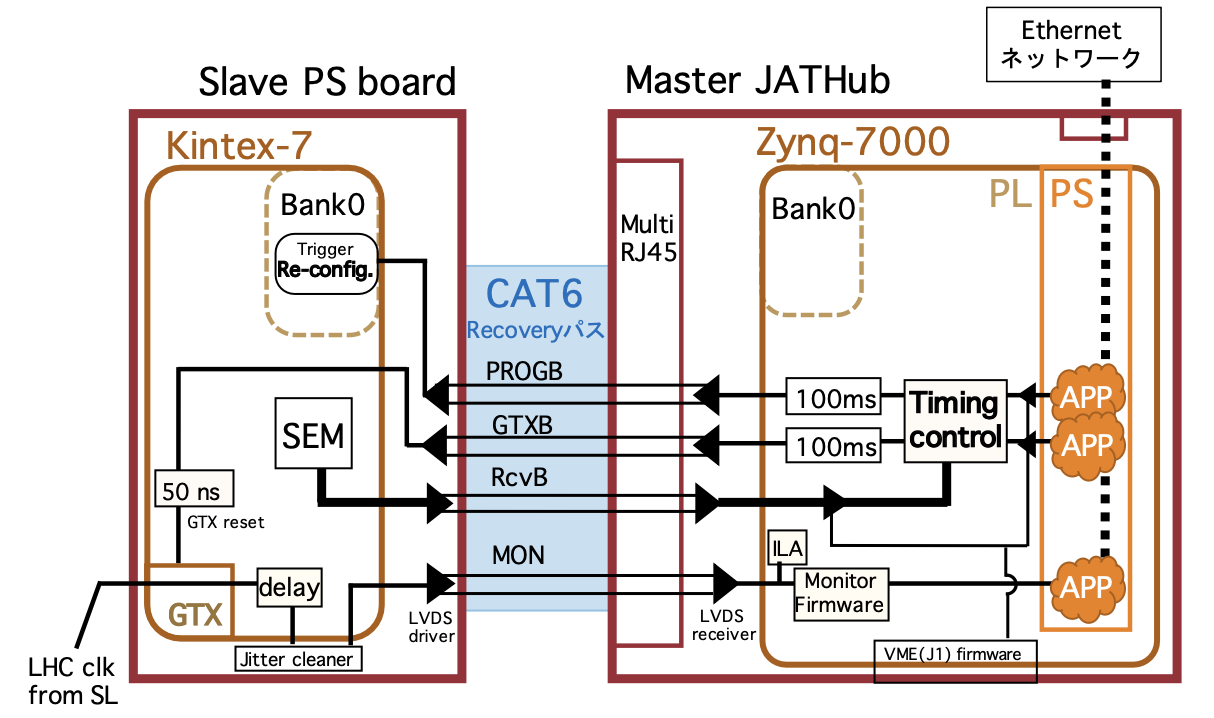
\includegraphics[width=16cm]{fig/QAQC/JATHubsem.png}
    \caption[JATHub によるリカバリー手続きの概要]{JATHub によるリカバリー手続きの概要\cite{mt_atanaka}。PS board に自己修復不可能な SEU 事象が発生した場合、RcvB線を通じてJATHubに救難信号が発出される。これを受信したJATHubはPROBG線をアサートすることでPS board FPGAの再コンフィギュレーションを行う。}
    \label{JATHubsem}
    \end{figure}

        \subsection*{Sector Logic  (SL) }
TGC BW 全7層分のヒットデータはSLに集められる。SLはVirtex UltraScale+ FPGAという大規模FPGAとZynq UltraScale+ MPSoCという2種類の集積回路を搭載している。Virtex UltraScale+ FPGAのデバイスはSL FPGAと呼ばれ、PS boardから受信したヒットデータを用いてトリガー計算を行う。また、SL FPGAはCTPからL0Aが発行されるまでのデータのバッファリングおよび後段への読み出しも担当する。Zynq UltraScale+ MPSoCはVirtex UltraScale+ FPGAやPS boardのコントロールマスターとして機能する。

\begin{figure} 
    \centering
    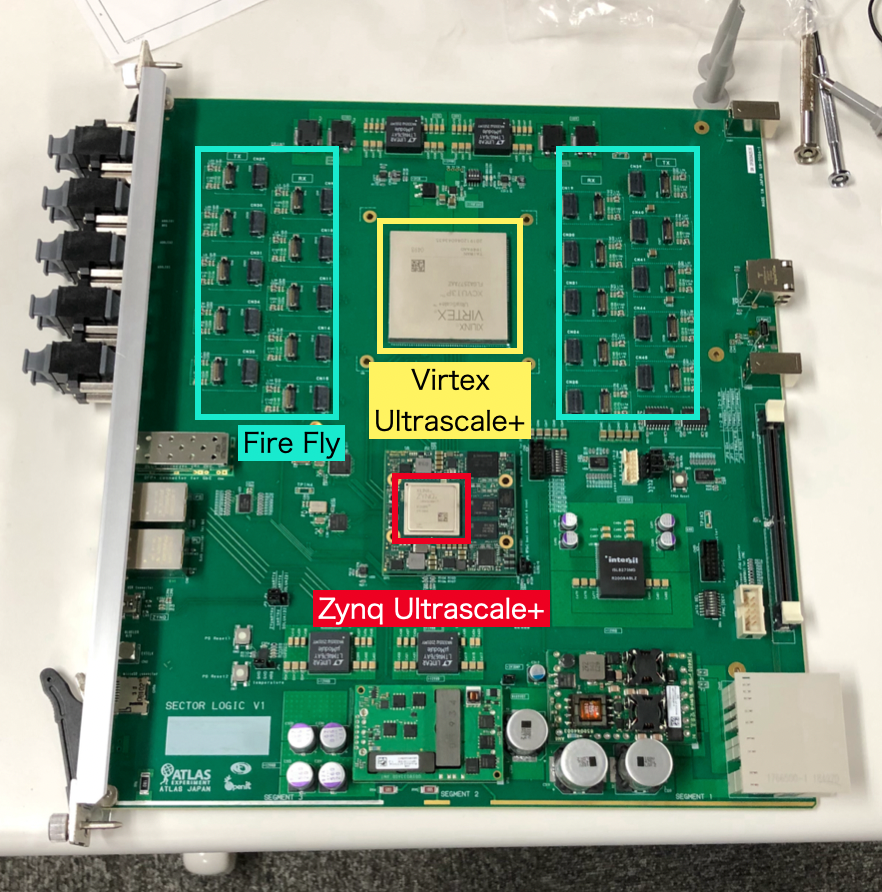
\includegraphics[width=14cm]{fig/Intro/TGC_SL.jpg}
    \caption[SL第一試作機の写真]{SL第一試作機の写真。SLはUSA15内のATCAクレートに設置される、ATCA規格のボードである。Virtex UltraScale+ FPGAとZynq UltraScale+ MPSoCという2種類の集積回路を搭載している。他のモジュールとのインターフェイスとして、FireFlyを送信用に10個、受信用に10個搭載している。1つのFireFlyは12リンクを束ねるため、合計120リンクの光通信が可能である。LANケーブルのインターフェイスであるRJコネクターも搭載しており、ethernetを介したネットワーク通信も可能である。}
    \label{TGC_SL}
\end{figure}

SLの第一試作機の写真を図\ref{TGC_SL}に示す。
SLはAdvanced Telecommunications Computing Architecture (ATCA)規格のボードである。ユーザーはATCAクレートのShelf managerからCERNで開発されたIntelligent Platform Management Controller  (IPMC) カードを介して、SLの電圧や温度のモニターや遠隔での電源操作を行うことができる。SLは外部とのインターフェイスとして電気信号を光信号に変換するためのFireFlyを送信用に10個、受信用に10個搭載している。それぞれが12レーンを束ねるため、送受信120リンクの光通信が可能である。1GイーサーネットケーブルのインターフェイスであるRJ45コネクターも搭載しており、イーサーネットを介したネットワーク通信も可能である。

1枚のSLはTGCの1/24セクターからの信号処理を担当し、合計31台のPS boardと接続する (BW用に29 枚、EI用に2 枚)。AsideとCsideを合わせて、合計で48枚のSLが設置される。以下にそれぞれの集積回路の機能の詳細を述べる。

    \subsubsection{SL FPGA}
SL FPGAに実装するファームウェアの概要を図\ref{SL_FW_overview}に示す。ファームウェアは大別してトリガー回路、読み出し回路、コントロール回路に分けられる。PS boardから光リンクを経由して送られるヒット情報は、トリガー回路および読み出し回路に入れられる。

\begin{figure} 
\centering
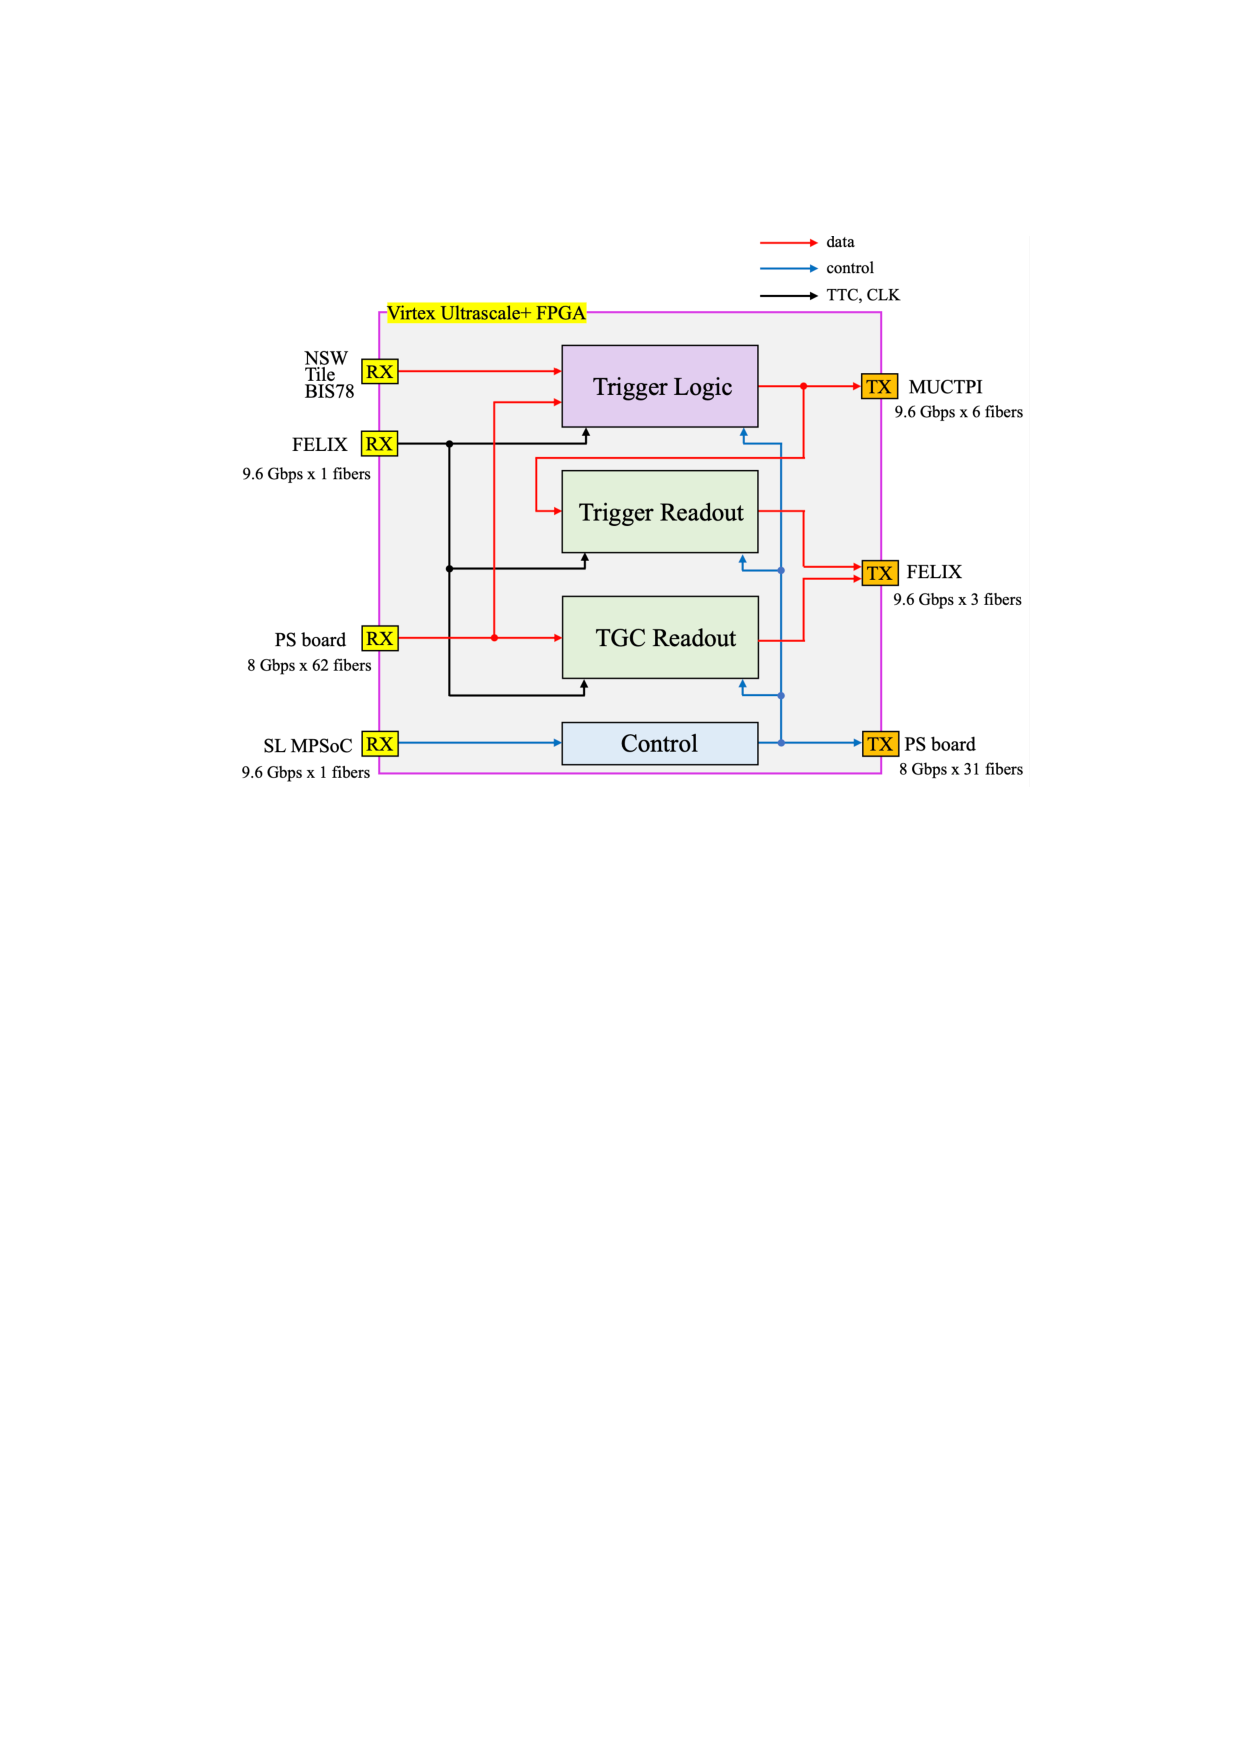
\includegraphics[width=16cm]{fig/Intro/SL_FW_overview.pdf}
\caption[SL FPGAに実装されるファームウェアの概要]{SL FPGAに実装されるファームウェアの概要\cite{mt_mishima}。SL FPGAは大別してトリガー回路、読み出し回路、コントロール回路に分けられる。トリガー回路はPS boardや磁場内部に位置する検出器からのヒットデータを受け取り、トリガー出力をMUCTPIに送信する。読み出し回路はPS boardからのヒットデータをバッファーし、FELIXからL0Aが出されたイベントのデータを取り出し、FELIXに送信する。コントロール回路はSL MPSoCからコントロール用信号を受け取り、各ロジックの制御を行う。}
\label{SL_FW_overview}
\end{figure}

トリガー回路は、PS boardから送られるBW 7層分のヒットデータを用いて\pt 判定を行なった後、エンドキャップトロイド磁石より内側にあるNSW、RPC BIS78、TIleカロリメーターからの情報も用いて、より精度の高い\pt の概算を行う。
SLで再構成されたミューオン飛跡の一部は、より精度の高い\pt 計算のためMDTTPへ送信される。MDTTPで処理された飛跡情報は、SLに送り返され、MDTTPに送られなかったものと合わせてMUCTPIへ送信される。
トリガー回路はこれまでにATLAS TGC グループの共同研究として開発が進められてきた。本研究では開発されたトリガーモジュールの全体ファームウェアへの統合および試験システムの開発を行った。この詳細は\ref{chap_TriggerIntegration}章、\ref{chap_TriggerTest}章で議論する。

読み出し回路は、PS board から受信したヒットビットマップとそのイベントに対応するトリガーデータをバッファーしておき、L0A が発行されたイベントのデータを選択的に後段へ転送する役割を担う。読み出されるデータにはゼロサプレスという圧縮処理が行われ、すべてのPS boardからのデータはイベントごとにパッキング  (Event Building) され、FELIXに送られる

コントロール回路は、LHC バンチ交差クロックと同期する必要のないスローな制御を担当する。MPSoCを起点にSL FPGA内のレジスタを操作することで、SLのトリガー・読み出しに関連するパラメーターの設定や、PS boardの制御を行う。

SL FPGAは4つのシリコンダイ (Super Logic Region, SLR) で構成される大規模なFPGAである。図\ref{ISEE_abstract}に示すように、隣接するSLRはSuper Long Line (SLL) と呼ばれる専用のワイヤーで接続されており、これを通じて信号の送受信が行われる。しかし、SLLを介した信号の伝搬は通常よりも大きなレイテンシーが生じる。さらに、SLLの位置はSLR内で物理的に固定されているため、SLLを過剰に使用する設計ではタイミング制約を満たすことが難しくなる。ファームウェアを物理的な制約 ( タイミング制約やリソース使用量など ) を満たしつつ効果的に実装するためには、I/Oや各種ロジックをFPGA上の適切な場所へ配置することが重要となる。

\begin{figure} 
\centering
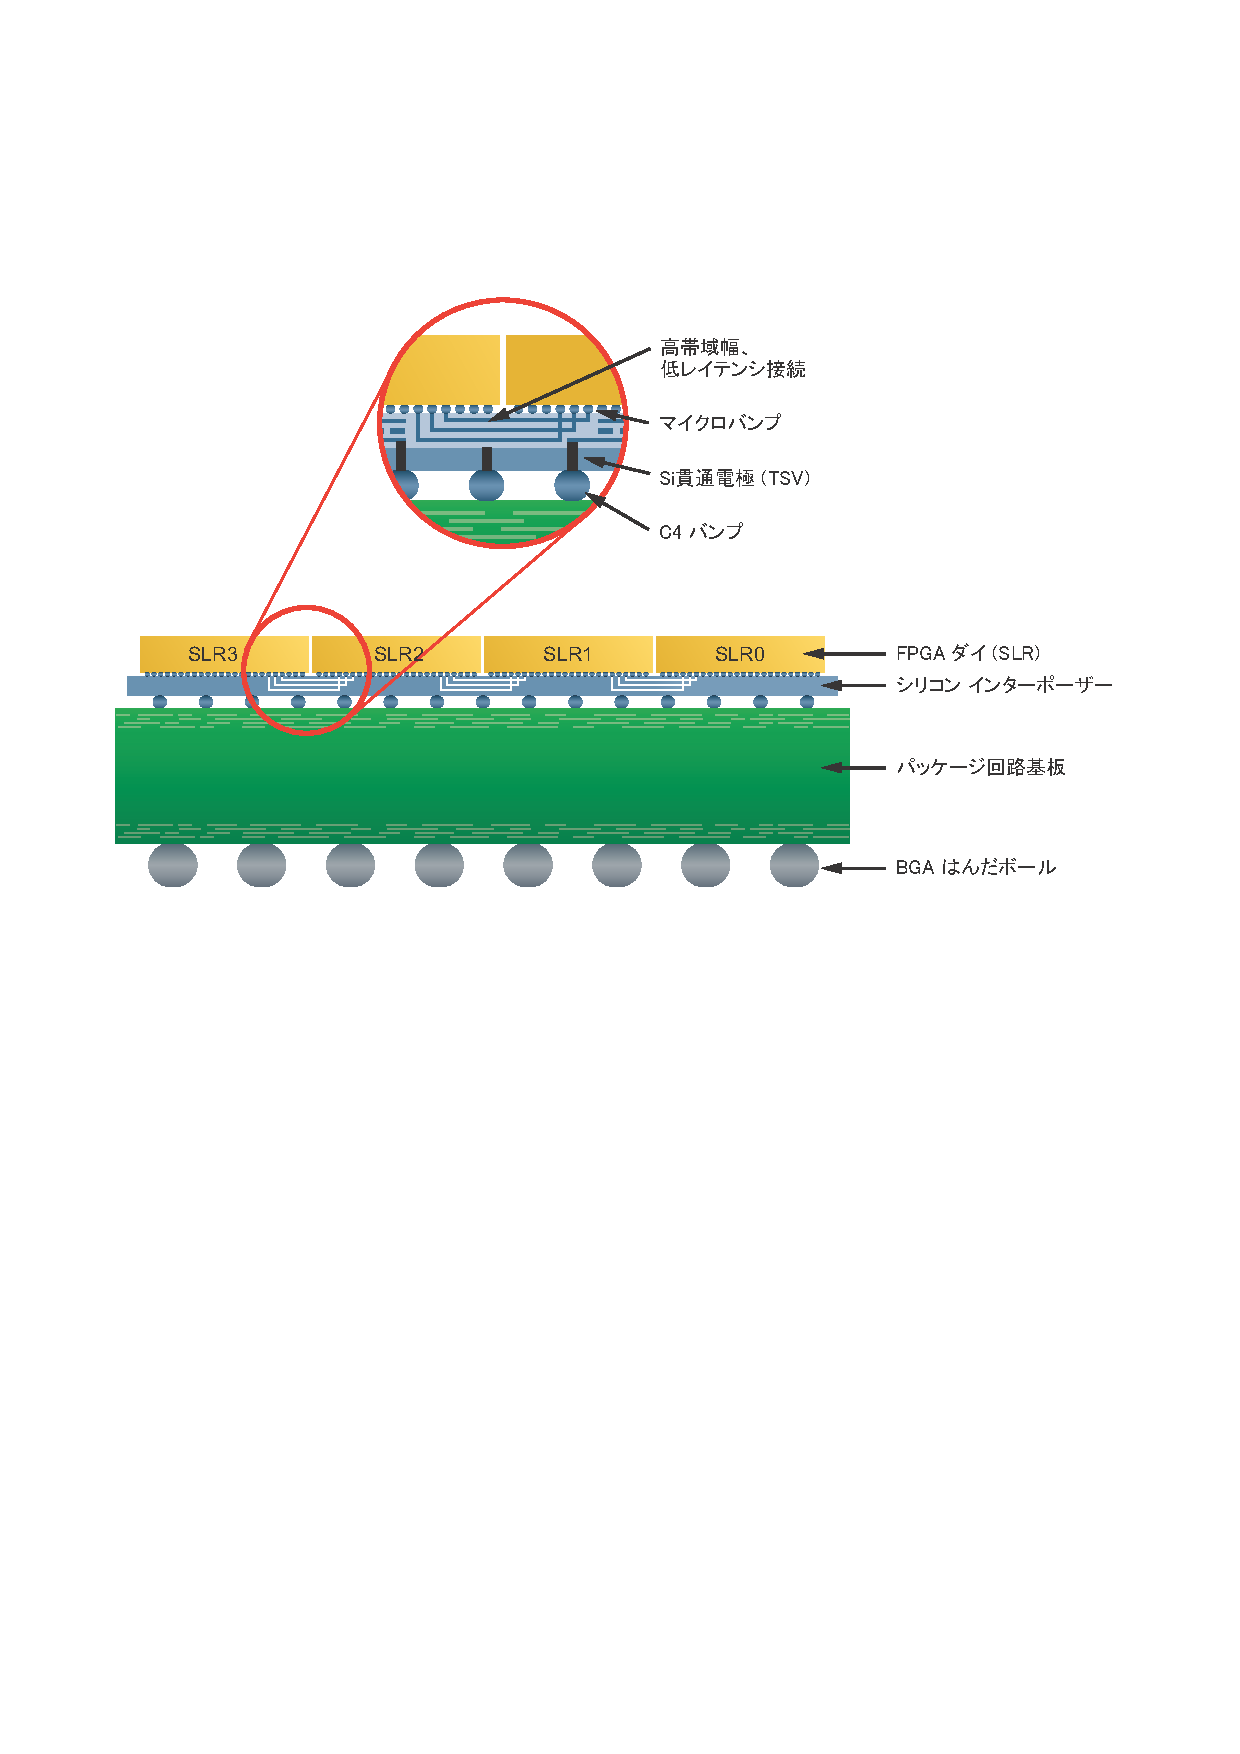
\includegraphics[width=16cm]{fig/Intro/ISEE_abstract.pdf}
\caption[SLRの概略図]{SLRの概略図。SL FPGAは4つのSLRで構成されており、隣接するSLRはSLLで接続されている。これによりSLR間で信号を送受信することができる。}
\label{ISEE_abstract}
\end{figure}

図\ref{SL_floor}に設計されたSL FPGAのフロアマッピングを示す。PS boardからのヒット信号はSLR0、SLR2、SLR3で受信され、磁場内部の検出器からの信号はSLR1で受信される。この配置に基づき、TGCのヒット信号のみを使用するトリガーロジック (TGC BW Coincidence) はそれぞれのSLRに配置され、Inner CoincidenceはSLR1に配置される。これにより、8,000 bit に及ぶPS board からのヒット信号はそれぞれのSLRで十分にデータ量が削減された後、SLR間で伝送される。
TGC BW Coincidenceは各SLRごとにトリガーセクターを分けて配置されており、SLR0にエンドキャップ$\phi\,0$、SLR2にエンドキャップ$\phi\,1$、SLR3にはフォワード領域のコインシデンスロジックが配置される。

SLからFELIXにヒットデータを送信するリンクはSLR3に配置される。SLRを超える信号をできるだけ小さくするため、読み出し回路はZero Suppressなどのデータ圧縮処理をそれぞれのSLR内で行い、SLR3で各SLRからのヒット信号を集め、イベントごとにパッキングする。また、MPSoCとSL FPGA間のチップ間通信リンクもSLR3に実装され、各SLRのレジスタ操作はSLR3を介して行われる。読み出し回路やコントロール回路などのFixed latencyでの実装が求められていないロジックでは、キューイングを適用しリソースを十分に節約した。

\begin{figure} 
\centering
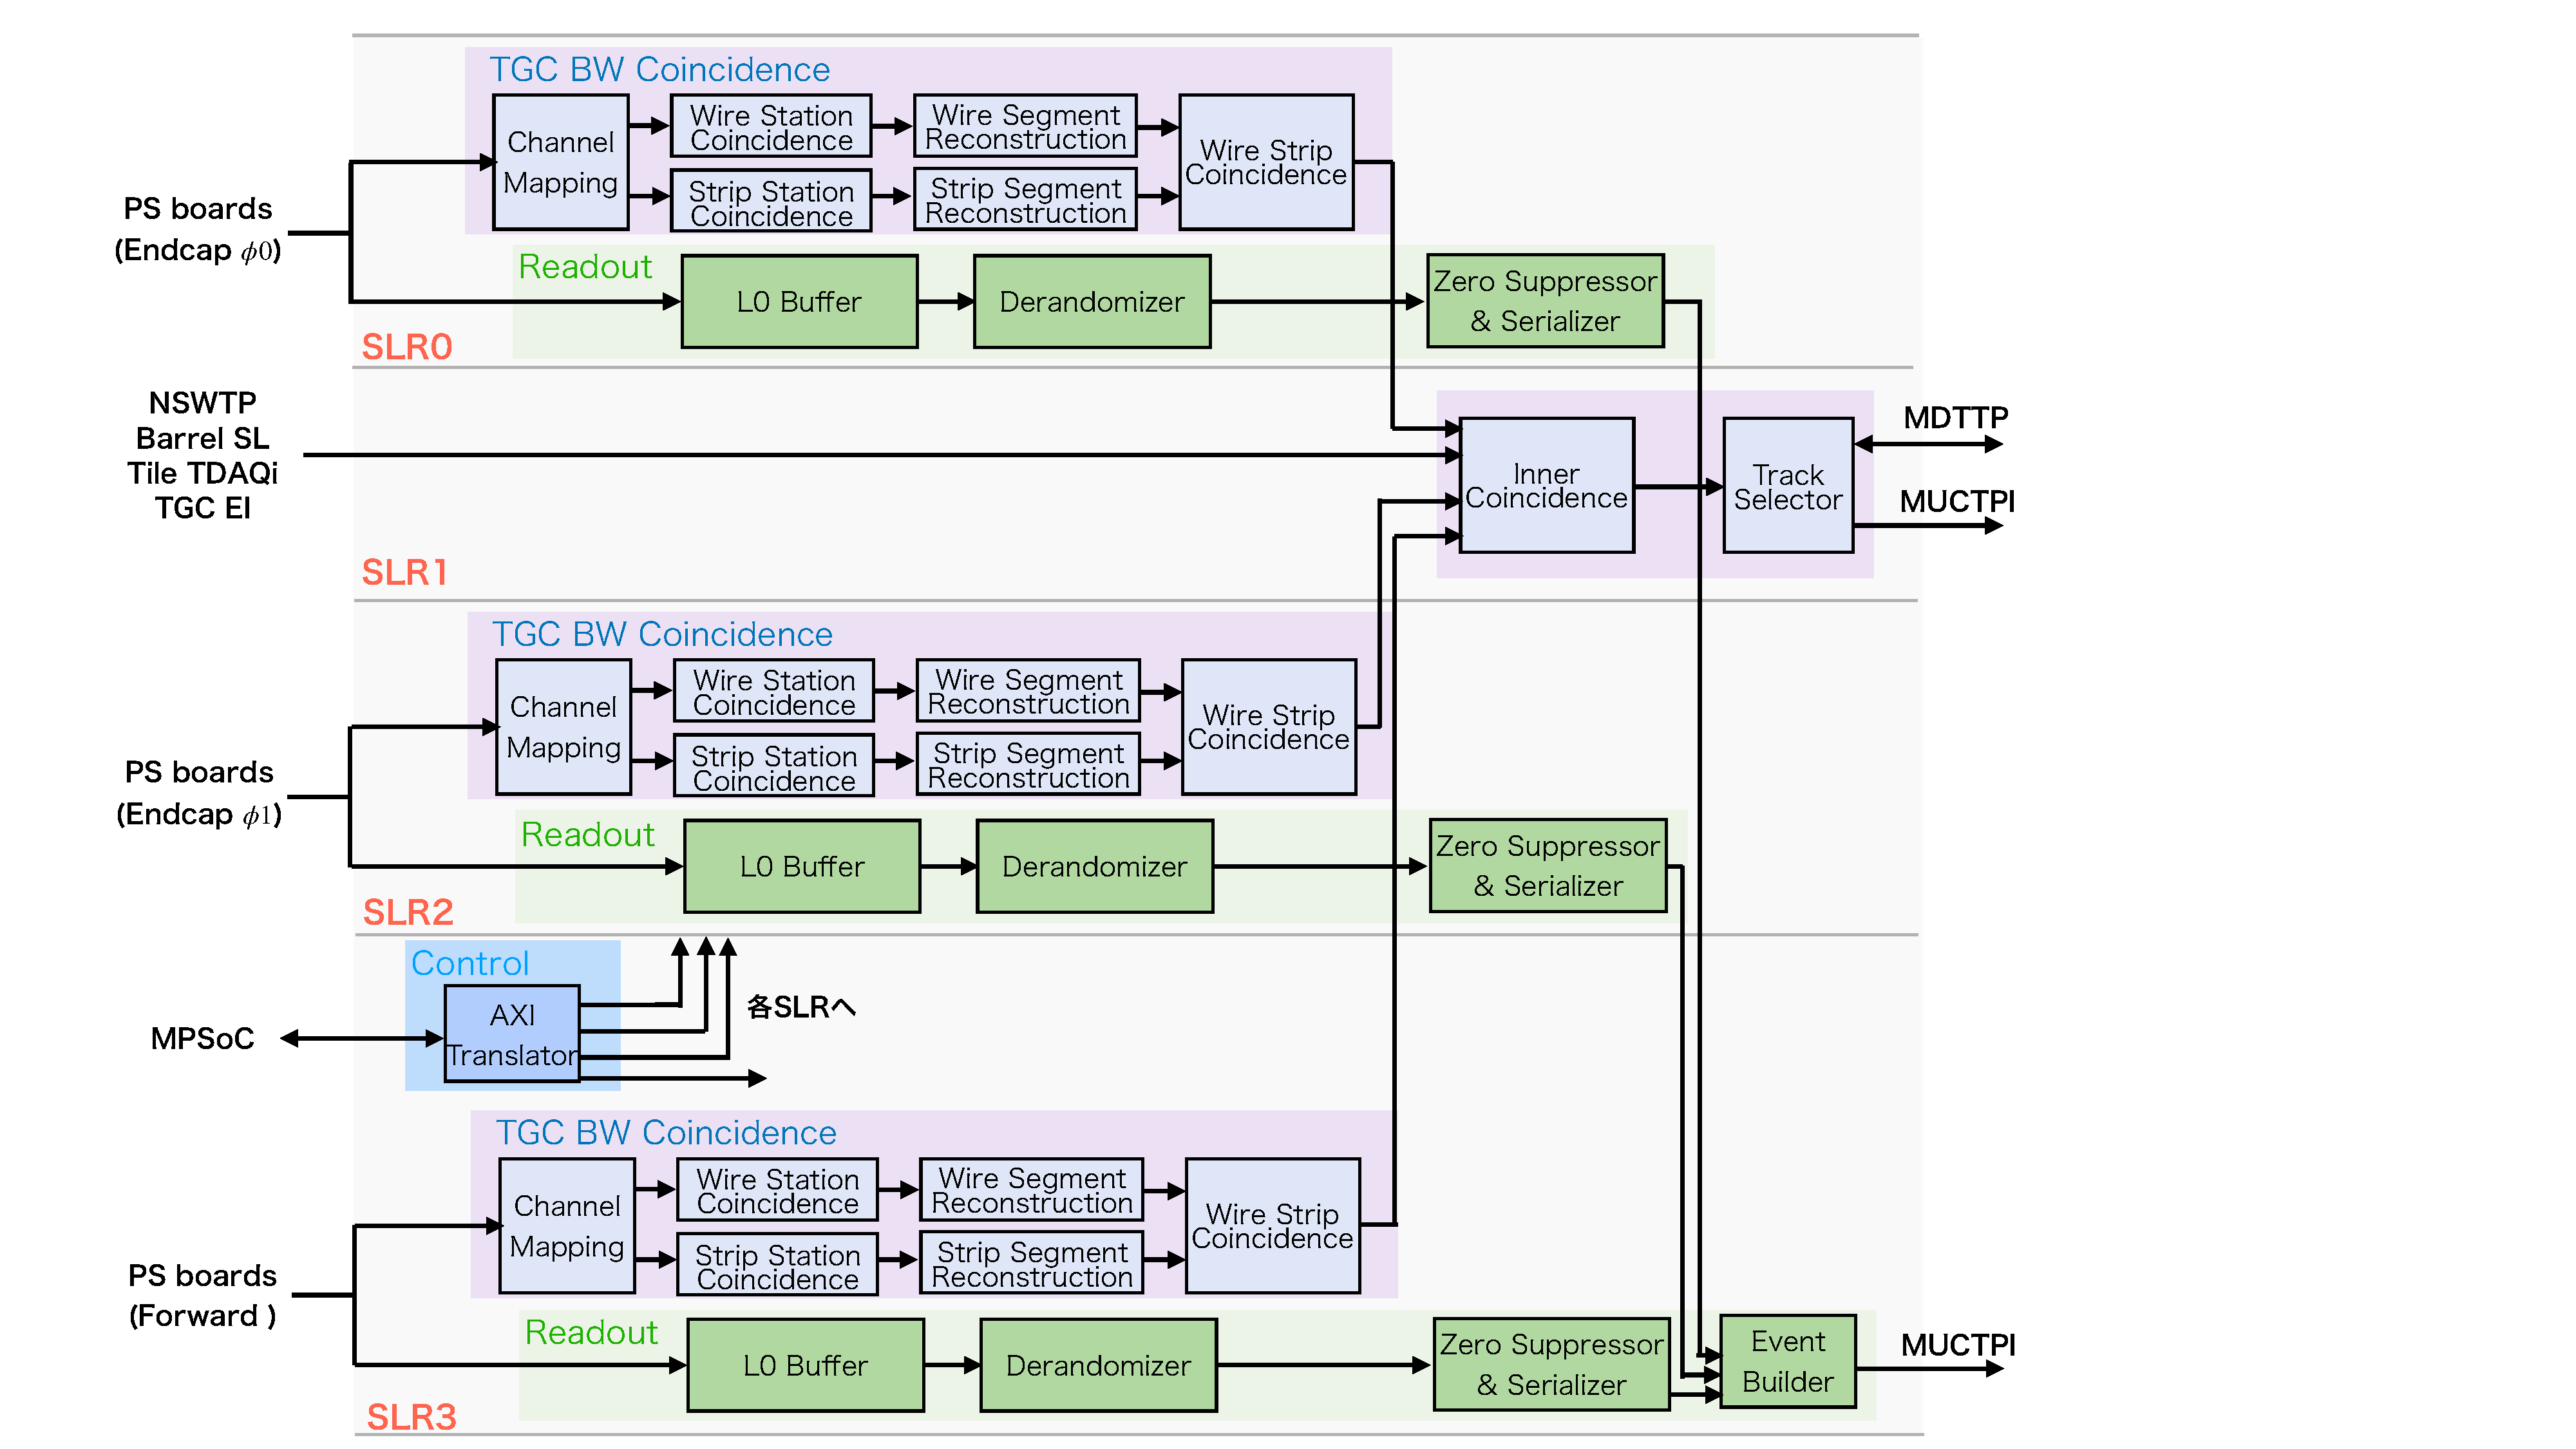
\includegraphics[width=16cm]{fig/Intro/SL_floor.pdf}
\caption[SL FPGAのフロアマップ]{SL FPGAのフロアマップ。PS boardからのヒット信号はSLR0、SLR2、SLR3で受信し、磁場内部の検出器からの飛跡情報はSLR1で受信する。それに合わせてSLR0、2、3にはTGC BW Coincidenceおよび読み出し回路の一部を配置し、SLR1にはInner Coincidenceを配置する。MPSoCとのインターフェイスはSLR3に配置し、これを介して各SLR内のレジスタ操作を行う。}
\label{SL_floor}
\end{figure}



    \subsubsection*{Zynq MPSoC}
Zynq MPSoCはSL FPGAおよびPS boardのコントロールマスターとして動作する。加えてATLASのTDAQシステムやDetector Control System (DCS)とのインターフェイスとしての役割も果たす。
Zynq MPSoCもPSとPLから構成されるシリコンデバイスである。PSにはプロセッサやメモリが搭載されていて、SLでは標準的なOSであるCentOS7を起動する。\footnote{Run 4で使用するOSは今後選定される。}

SLのMPSoCはEnclustra社が開発しているMercury XC5メザニンカードに搭載されている。このメザニンには高速通信を行うためのIOが搭載されており、SL FPGAとMPSoCは2レーンの高速シリアル通信を行うことができる。これにより、MPSoCからSL FPGAのコントロールやSL FPGAからMPSoCへのデータ読み出しを行なっている。
Mercury XU5には他にも、DDR4 SDRAMやeMMC、Gigabit Ethernet PHY、USB PHY、QSPI フラッシュメモリなどが搭載されている。市販のメザニンを活用することで、SLボードの開発コストを下げることに加え、メンテナンスを容易にすることができる。Mercury XU5メザニンカードの構造と、SLボード上における接続関係を図\ref{SL_mezanin}に示す。

\begin{figure} 
\centering
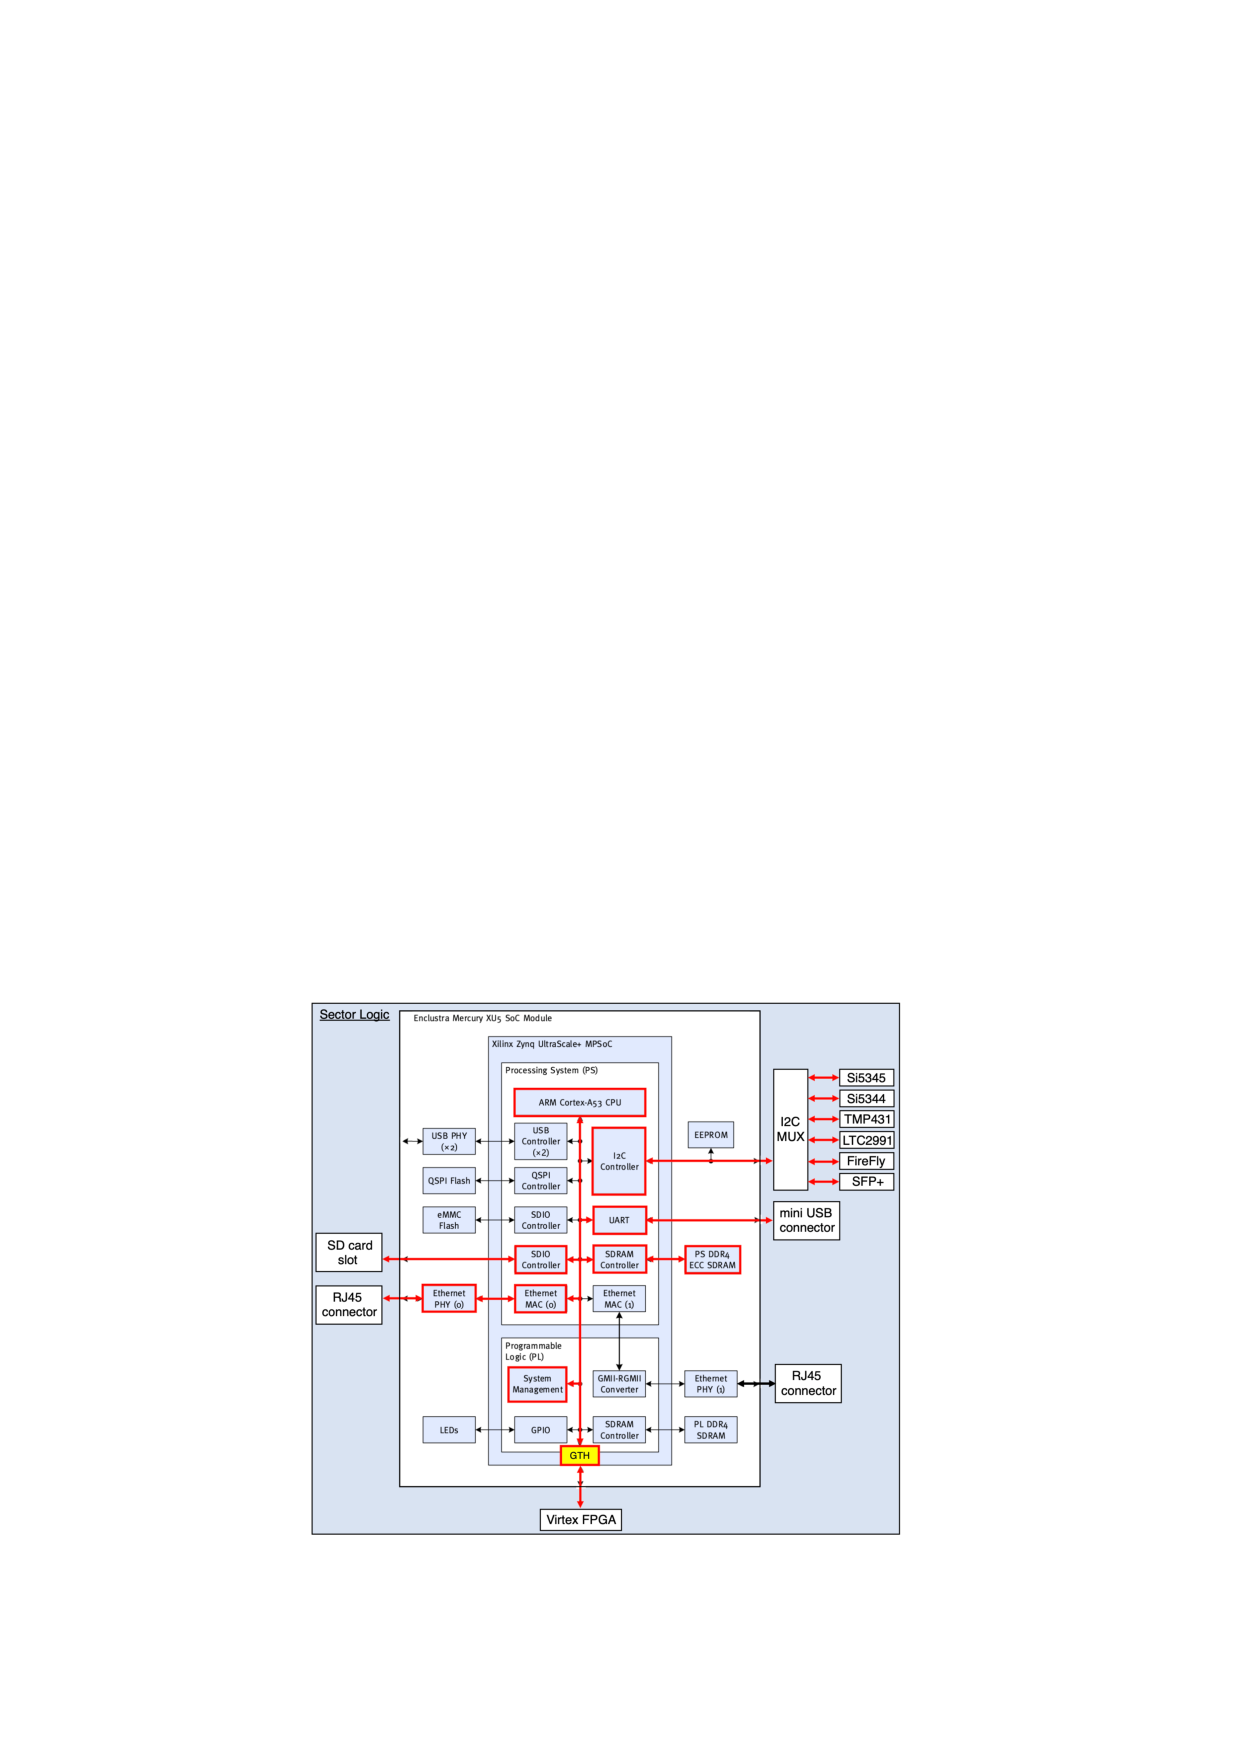
\includegraphics[width=16cm]{fig/Intro/SL_mezanin.pdf}
\caption[Mercury XU5 メザニンカードの構造とSLボード上における接続関係]{Mercury XU5 メザニンカードの構造とSLボード上における接続関係\cite{mt_mishima}}
\label{SL_mezanin}
\end{figure}
\chapter{高輝度LHC-ATLAS実験に向けたエンドキャップミューオントリガーの統合}
\label{chap_TriggerIntegration}
高輝度LHC-ATLAS実験において、エンドキャップ部トリガーロジックは大規模論理回路としてSL FPGA上に実装される。トリガーロジックはこれまで、東京大学、京都大学、名古屋大学をはじめとするATLAS TGC JAPAN グループの共同研究として開発が進められてきた。本章ではまず、トリガーロジック開発の流れを説明する。次にこれまでに開発されたトリガーロジックのコンセプトとHDL実装について述べた後、本研究で行なった統合作業について述べる。

\section{トリガーロジック開発の流れ}
\label{sec_TriggerTestSystem}
本節では、高輝度LHC-ATLAS実験に向けたエンドキャップ部ミューオントリガー回路の開発流れを説明し、トリガー開発全体の流れにおける本研究の位置づけを説明する。図\ref{Trigger_flow}にトリガーロジックの開発フローを示す。トリガーロジックは最終的にバックエンドエレクトロニクスであるSLのFPGA上でデジタル回路として稼働するが、それまでにコンセプトの設計、モジュールごとのHDL実装、全体ファームウェアへの統合という3ステップで開発が進められてきた。また、それぞれの工程において検証システムも同時に構築することで、期待した性能をもつトリガーロジックが実現できていることを確かめながら、着実に開発が進められている。

\begin{figure} 
\centering
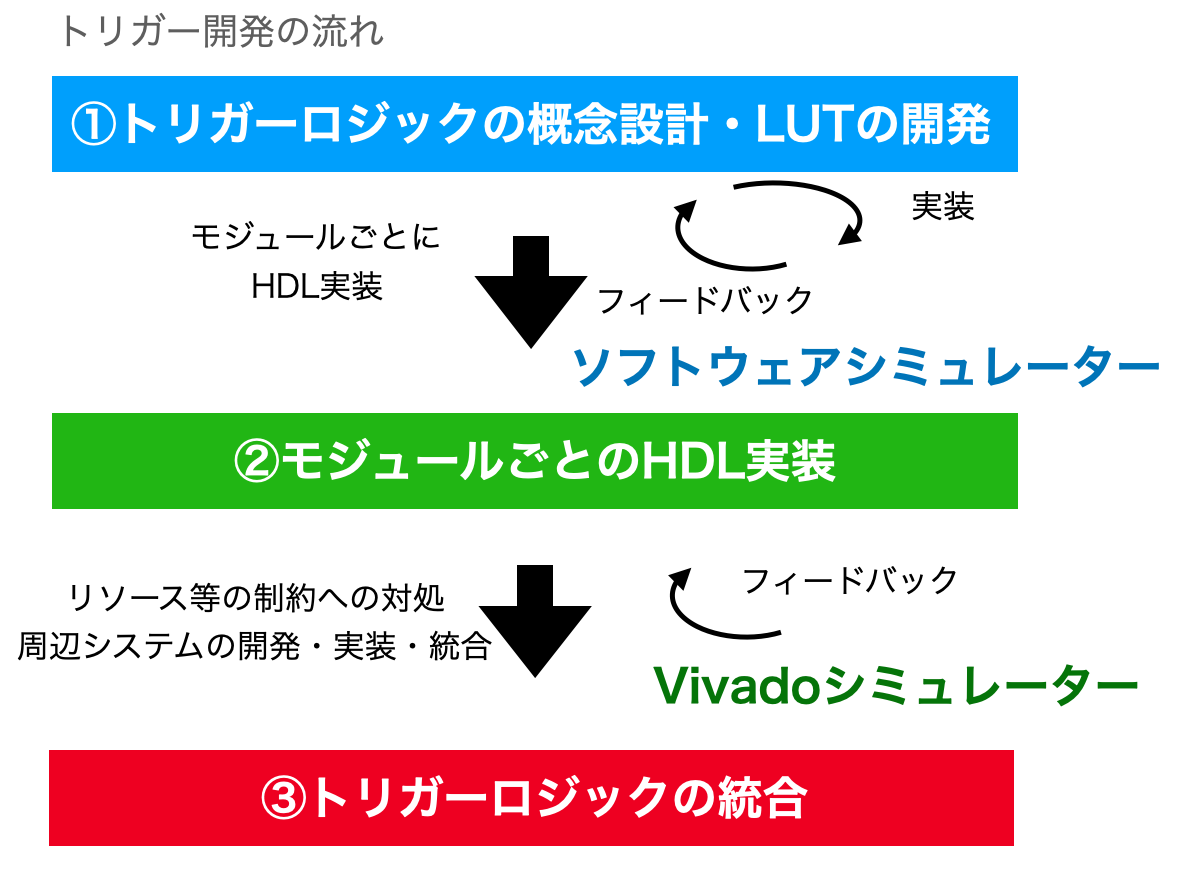
\includegraphics[width=16cm]{fig/SL/Trigger_flow.png}
\caption[TGCトリガー開発の流れ]{TGCトリガー開発の流れ。}
\label{Trigger_flow}
\end{figure}

\subsection*{トリガーロジックの概念設計}
トリガーの開発は、まず高輝度LHC-ATLAS実験におけるL0 Trigger systemの要求を満たすよう、概念的な設計を行う。L0 Trigger systemの要求には具体的にトリガー効率、再構成した角度分解能、トリガーレート、トリガーレイテンシーなどが含まれる。Run3ロジックの例でいうと、SLBでM1、M3間のコインシデンスをとり、HPTで3ステーションのコインシデンスをとり、SLでWireとStripのコインシデンスをとる、というようなグローバルな設計から、複数なヒットがあった場合にどのような優先順位で飛跡候補を選ぶか、という具体的な設計までこの段階で行われる。

設計されたロジックを、より具体的なデザインに落とし込み、性能を評価していく作業にはソフトウェアシミュレーターを用いる。ソフトウェアは開発が容易で、ロジックの実装→性能評価→ロジックの修正→…という開発サイクルを素早く回すことができる。そのため、グローバルなデザインを決めていく初期の開発には有用である。さらに、パターンマッチングに利用されるLUTもロジックの設計と同時にソフトウェア的に開発される。

\subsection*{モジュールごとのHDL実装}
コンセプト設計が固まったあとには、そのロジックを電子回路上で動作させるためにHardware Description Language ( HDL ) の記述に落とし込む作業が行われる。ミューオントリガー回路は複数のトリガーモジュールをパイプライン的に接続することで実現するため、まずは個々のモジュールごとにHDL実装が進められた。この工程ではロジックをRegister Transfer Level (RTL) として解釈し直すことに加え、そのロジックをFPGAの物理制約を満たした形で実現するための最適化が行われる。具体的には、ステーション間コインシデンスで使用するLUTはFPGA上のRAMに格納するため、使用するLUTのサイズは物理的な制限がかかる。その中で、どのようにパターンマッチングを行う最小領域 (Unit ) を設定するべきか、などの最適化研究はこの段階で行われた。

開発されたHDLの動作検証および実装されたトリガー回路の性能評価には、Vivado シミュレーターが用いられる。Vivado シミュレーターとはHDLで記述されたデジタル回路の動作を逐次的にエミュレートトするソフトウェアツールである。デジタル回路に含まれる全ての信号の遷移を厳密にシミュレーションし、任意の時間の任意の信号線をプローブすることができる。

\subsection*{トリガーロジックの統合}
最後にHDLで実装されたトリガーモジュールをSL ファームウェア全体の中で動作させる統合作業を行う。トリガー回路をシステムの中で動作させるためには、PS boardや磁場内部の検出器からトリガーロジックへの入力を作成するインターフェイス、LUTの書き込みやタイミング制御を行うコントロール機能、トリガー出力をバッファーおよび成形する読み出し機能が必要である。周辺機能の実装と接続を丁寧に行い、1つの大規模論理回路として統合していく。

HDLで統合したロジックはVivadoによるインプリメンテーション\footnote{Vivadoのインプリメンテーションプロセスは、主に1. ロジック最適化、2.デザイン配置、3.配置後のデザインの物理最適化、4. デザインの配線、5. 配線後のデザインの物理最適化、6 ビットストリームの生成で構成される。}プロセスを経て、ハードウェア上で動作させることができる。これにはファームウェア全体を通じて、リソース使用量やタイミング制約などの物理制約を満たす必要があり、SLのような大規模論理回路ではこれに向けた最適化が必要不可欠となる。

\subsection*{本研究の立ち位置}
これまでの先行研究で各モジュールのHDL実装およびVivado シミュレーターを用いた性能評価研究が完了している。そこで本研究では、まずトリガーロジックの統合に取り組む。この詳細は\ref{sec_TriggerIntegration}節で述べる。また、本研究では実際に実機上で動作しているトリガー回路を、本番運用に近い形で試験することができる次世代的なシングルボード試験システムを開発した。これにより、実機上で動作するトリガー回路を詳細に調査、デバッグすることが可能となり、トリガーロジックの本番運用に向けた重要なインフラが実現した。この詳細は\ref{chap_TriggerTest}章で述べる。

\section{高輝度LHC-ATLAS実験におけるトリガーロジックのコンセプトとHDL実装}
\label{sec_Phase2TriggerLogic}
本節では先行研究で開発されたトリガーロジックのコンセプト設計と、HDLでの実装について述べる。

高輝度LHC-ATLAS実験でのミューオントリガー回路の全体像を図\ref{Trigger_over}に示す。前章で述べたように、高輝度LHC-ATLAS実験におけるSLは1/24セクター内のTGC BW 7層からのヒットビットマップを、トリガーをかけることなくすべて受信するようになる。そのため、Run3でSLBボード、HPTボード、SLで分割されていたトリガーロジックは、すべてSLのFPGA上に実装されるようになる。

\begin{figure} 
\centering
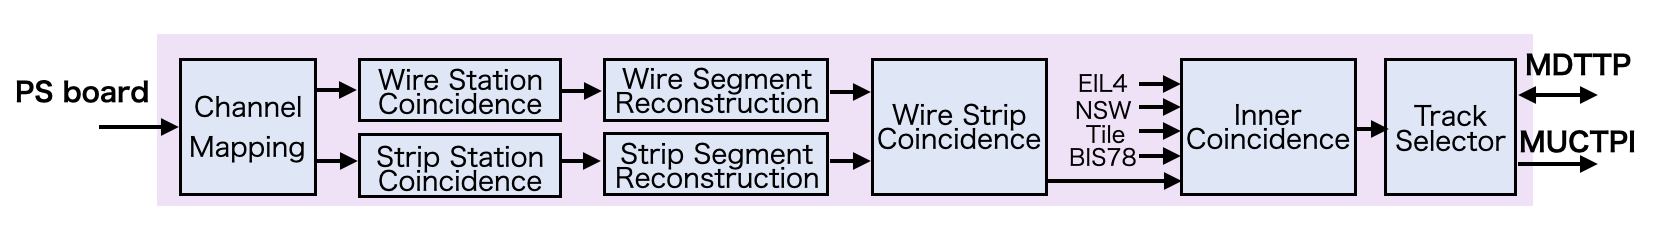
\includegraphics[width=16cm]{fig/SL/Trigger_over.png}
\caption[トリガー回路の全体像]{トリガー回路の全体像}
\label{Trigger_over}
\end{figure}

SL FPGAに実装されるトリガーロジックはChannel Mapping、Station Coincidence、Segment Reconstruction、Wire Strip Coincidence、Inner Coincidence、Track Selectorという6つのモジュールをパイプライン的に接続することで実現される。
PS board から受信するヒットビットマップはChannel Mapping でコインシデンスロジックの入力に適した形へと並び替えられる。入力されたヒットデータはStation CoincidenceおよびSegment reconstructionでワイヤー、ストリップそれぞれでコインシデンスがとられる。Segment Reconstruction ではTGCのヒットから再構成される飛跡と無限運動量飛跡のなす角d$\theta$、d$\phi$が計算される。Wire Strip coincidenceは、Wireで再構成されたd$\theta$とStripで再構成されたd$\phi$のコインシデンスを取ることで、横方向運動量閾値\pt を概算する。ここまでのコインシデンスロジックをまとめてTGC BW コインシデンスと飛ぶ。TGC BW コインシデンスで再構成されたミューオン飛跡候補はInner Coincidenceにて、磁場内部の検出機(NSW、BIS78、RPC、EIL4 TGC、Tile カロリメーター)とコインシデンスが取られ、フェイクトリガーの削減および\pt 精度の向上が実現される。Inner Coincidenceは最大112個の飛跡候補を出力する。最後にTrack selectorで、112個の飛跡候補から\pt の大きい順に最大6つの飛跡候補が選別される。そのうち3つはMDTTPに転送され、MDTTTPにてさらに高い精度でミューオンの運動量を計算された後、その結果を再度受け取る。SLはMDTTPから受信した飛跡候補3つと、MDTTPへ転送しなかった飛跡候補3つ合わせて6つをMUCTPIに転送する。以下にそれぞれのロジックの詳細と、HDLへの実装方法を説明する。

\subsection{Channel Mapping}
\subsubsection*{コンセプト}
Channel MappingではPS board から受信するTGC BW 全チャンネルのヒット情報 (128 bit x 62 link)を、飛跡再構成に先んじてトリガー入力に適したフォーマットへとマッピングする処理を行う。この工程ではただチャンネルを並び変えるだけでなく、TGC検出器のジオミトリに合わせて設計されたフロントエンドのチャンネル構造をトリガーロジックとして取り扱いやすいものへと変換する。TGC BW のエンドキャップ領域は$\eta$方向にM1は4つ、M2、M3は5つのチェンバーで構成されており、それぞれ不完領域がないようにオーバーラップを持って設置されている。このオーバーラップ領域では一つのミューオンのヒットを重複してカウントする可能性があるため、トリガーに入力する際にはWIred ORと呼ばれる統合処理を行う。また、ストリップのコインシデンスはチェンバーごとに行われるが、ミューオン飛跡が$\eta$方向に曲げられ、複数のチェンバーに跨ってヒットを残した場合には、コインシデンスをとることができない。これに対処するため、とあるM3チェンバーとのコインシデンスと担当するM1及びM2チェンバーでは図\ref{}のようにORを取った上で、コインシデンスが取られる。

\begin{figure} 
\centering
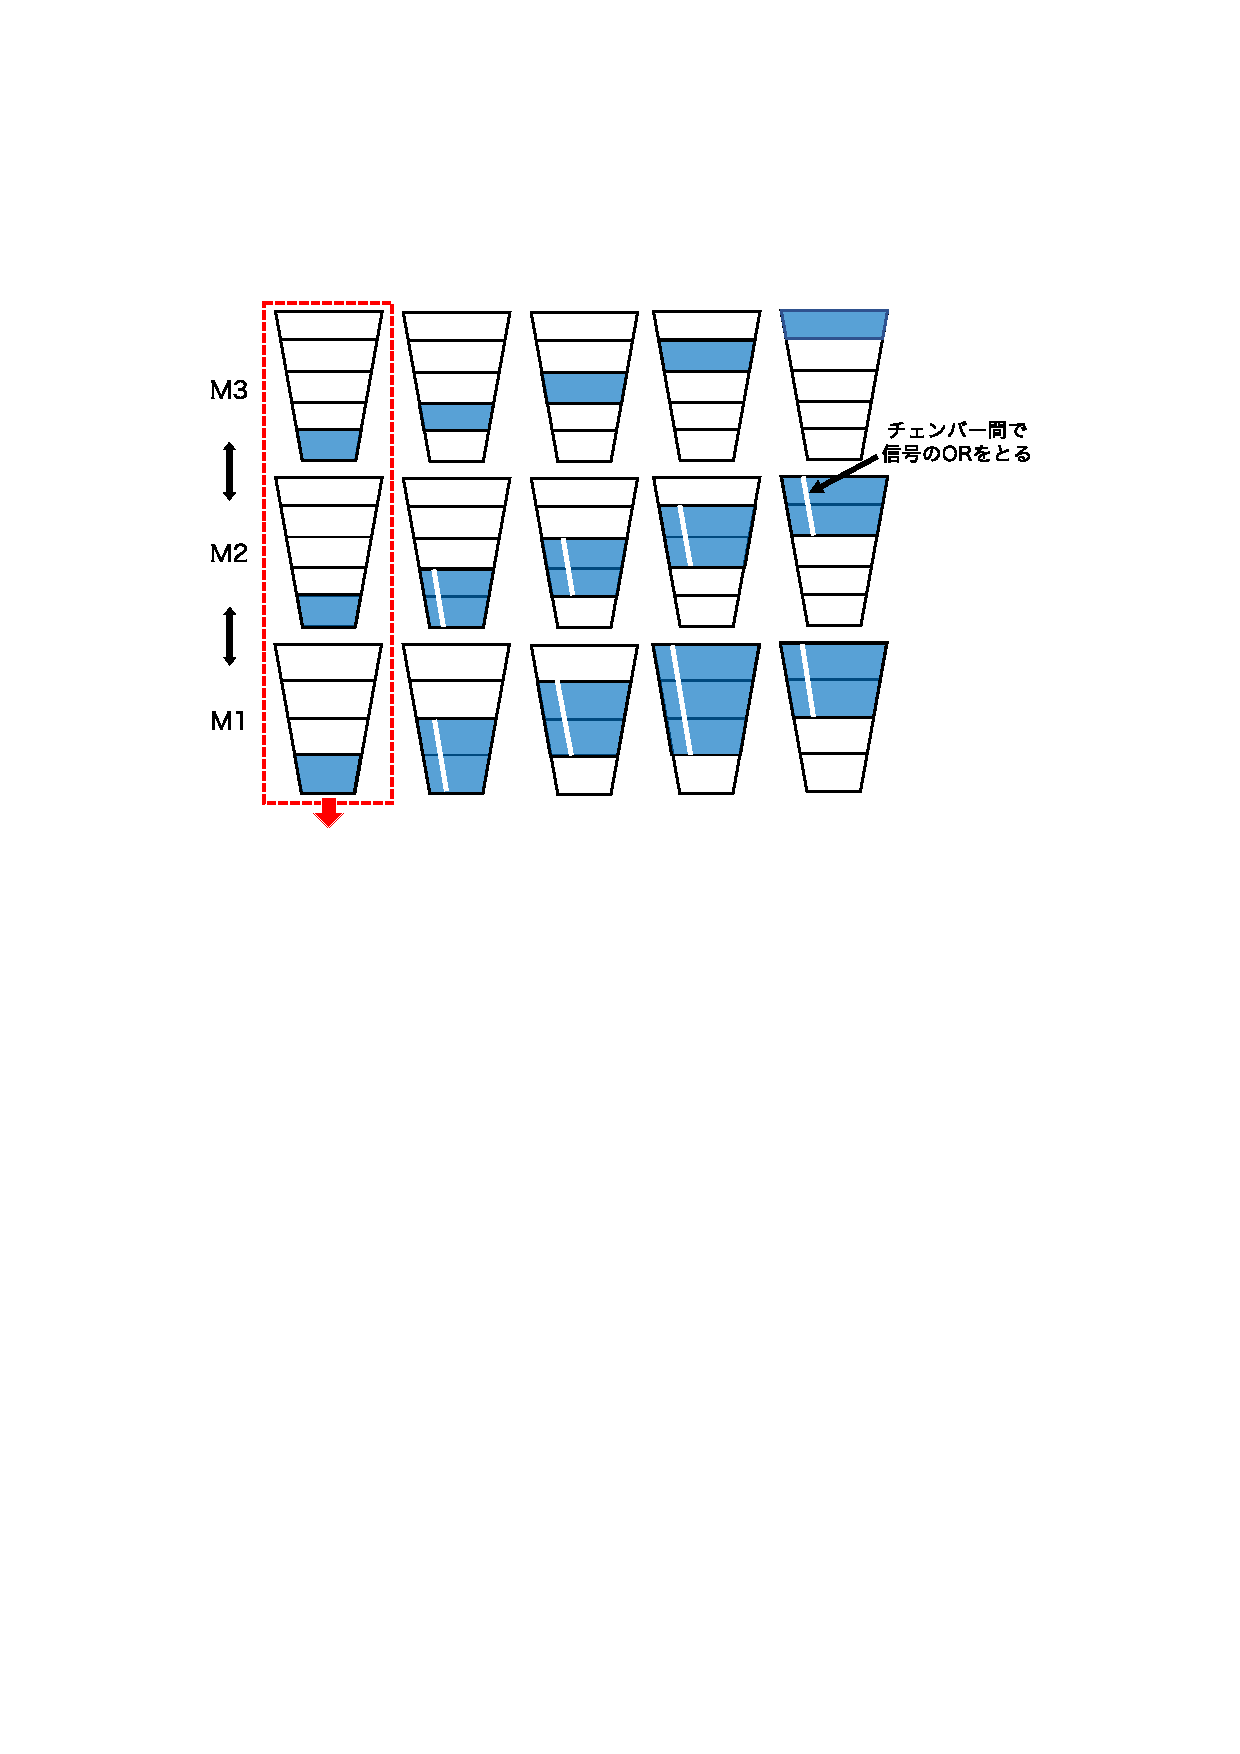
\includegraphics[width=16cm]{fig/SL/Channel_Mapping.pdf}
\caption[]{ストリップにおけるチェンバー間のORの取り方。M3チェンバーとのコインシデンスと担当するM1及びM2チェンバーではORをとった情報を後段に流す。\cite{mt_kawamoto}}
\label{fig_CTA}
\end{figure}

\subsubsection*{HDL実装}
Channel MappingモジュールはHDLでは単純な配線とOR回路で実装されている。

\subsection{Station Coincidence}
\subsubsection*{コンセプト}
図\ref{}にStation Coincidenceの概要を示す。TGC検出器はスタッガリング構造を取っており、ステーション内のワイヤーは互いに$\eta$方向にずらして、ストリップは互いに$\phi$方向にずらして設置されている。M1、M2、M3の各チャンネルが重複してカバーする$\eta$領域、$\phi$領域を代表点として定義する。Station CoincidenceはM1 3層、M2 2層、M3 2層のヒットチャンネルを入力として、コインシデンスが取れた代表点を出力する。これによりデータ量を落としながら、より位置分解能を上げてミューオンの位置情報を決めることができる。

\begin{figure} 
\centering
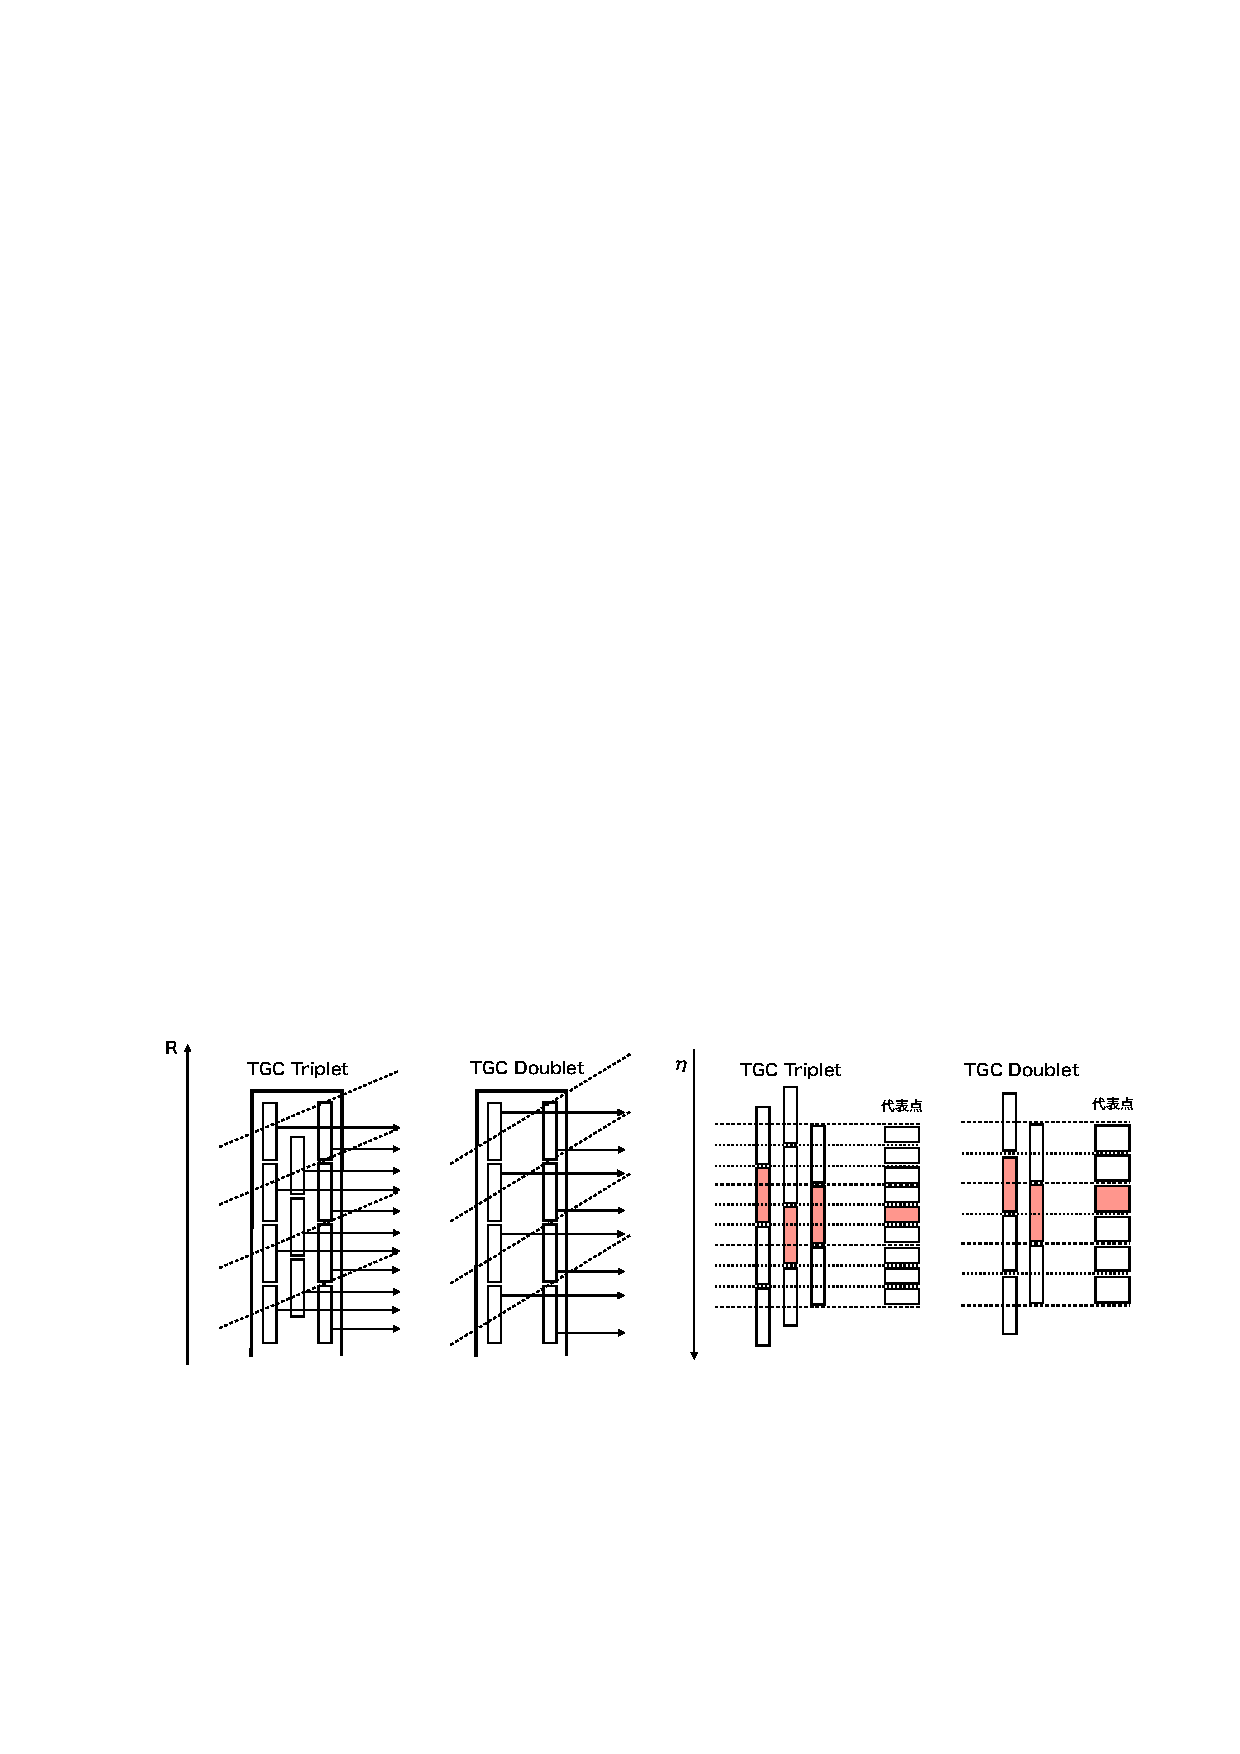
\includegraphics[width=16cm]{fig/SL/Concept_station.pdf}
\caption[Station コインシデンスの概要]{Station コインシデンスの概要\cite{mt_mino}。スタッガリング構造をとっている。}
\label{Concept_station}
\end{figure}

\subsubsection*{Wire Station CoincidenceのHDL実装}
このモジュールの駆動クロックは、LHCバンチ交差クロックに同期した40 MHzクロックでレイテンシーは1クロックチック ( 25 ns )である。
Wire Station Coincidenceおよび\ref{subsec:segment_reco}節で説明するWire Segment ReconstructionはUnit、Subunitと呼ばれる単位領域でトリガーセクターを分割して、Subunitごとに並列にコインシデンス処理を行う。UnitやSubunitは先行研究にて、とあるM3チャンネルにヒットを残した\pt 5 GeVのミューオンを再構成するのに必要な、M1、M2チャンネルを網羅するよう定義された。

ワイヤーロジックではエンドキャップ領域を37分割、フォワード領域を16分割したものをUnitと定義する。図\ref{StationCoin_unit}にユニットの構造を示す。1つのユニットはM1ステーションの96 代表点、M2ステーションの32代表点、M3ステーションの16代表点をカバーする。また、1つのユニットを4等分するようにしてSubunitが定義されている。

\begin{figure} 
    \centering
    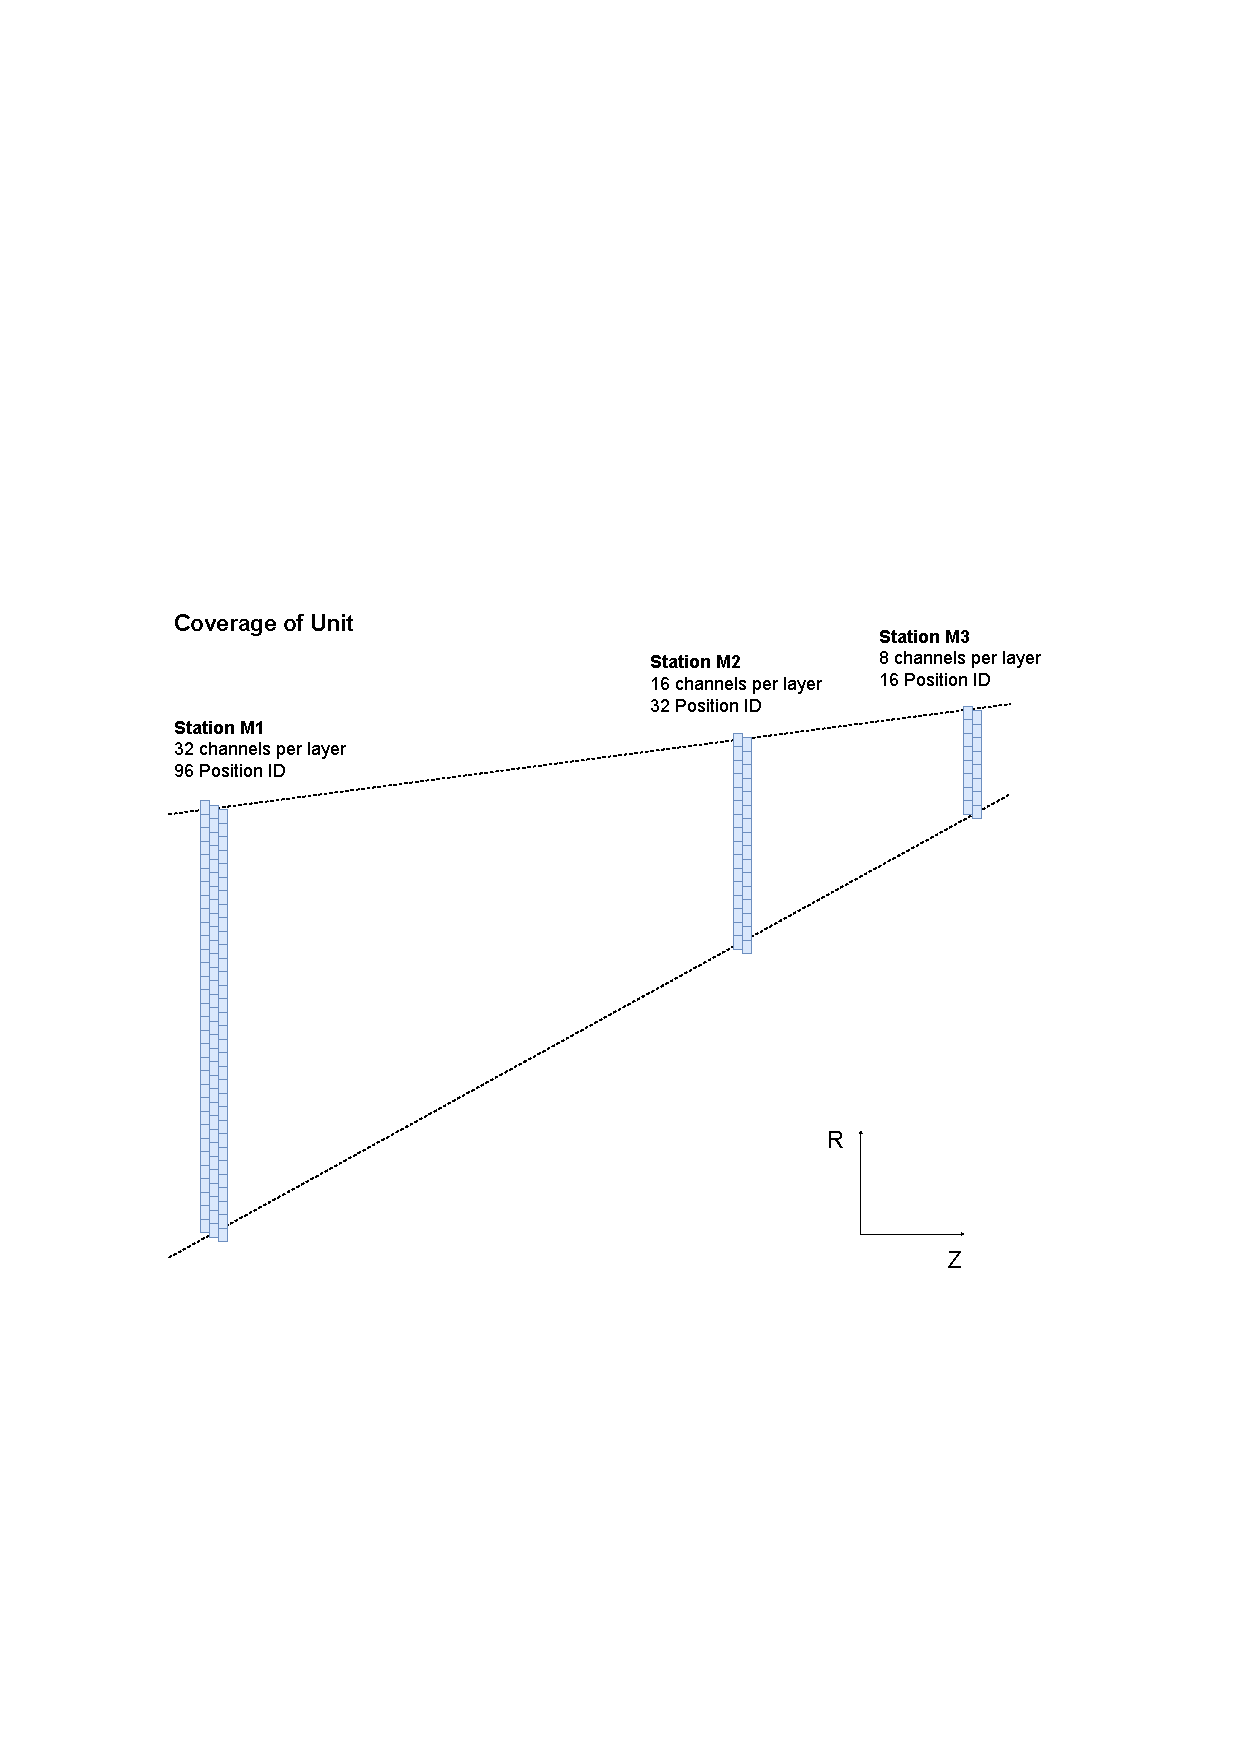
\includegraphics[width=16cm]{fig/SL/StationCoin_unit.pdf}
    \caption[Wire Station Coincidence および Wire Segment Reconstruction におけるユニット]{Wire Station Coincidence および Wire Segment Reconstruction におけるユニット}
    \label{StationCoin_unit}
\end{figure}

M1ステーションにおけるコインシデンスロジックの概要を図\ref{StationCoin_wire}に示す。ステーションコインシデンスはHDLではandとorの組み合わせ回路として実装される。3層中3層にヒットがあった場合に代表点を出力する3/3コインシデンス、2層にヒットがあった場合の2/3コインシデンス、1層にヒットがある場合の1/3コインシデンスが独立に用意されており、それぞれが並列に動作する。

\begin{figure} 
    \centering
    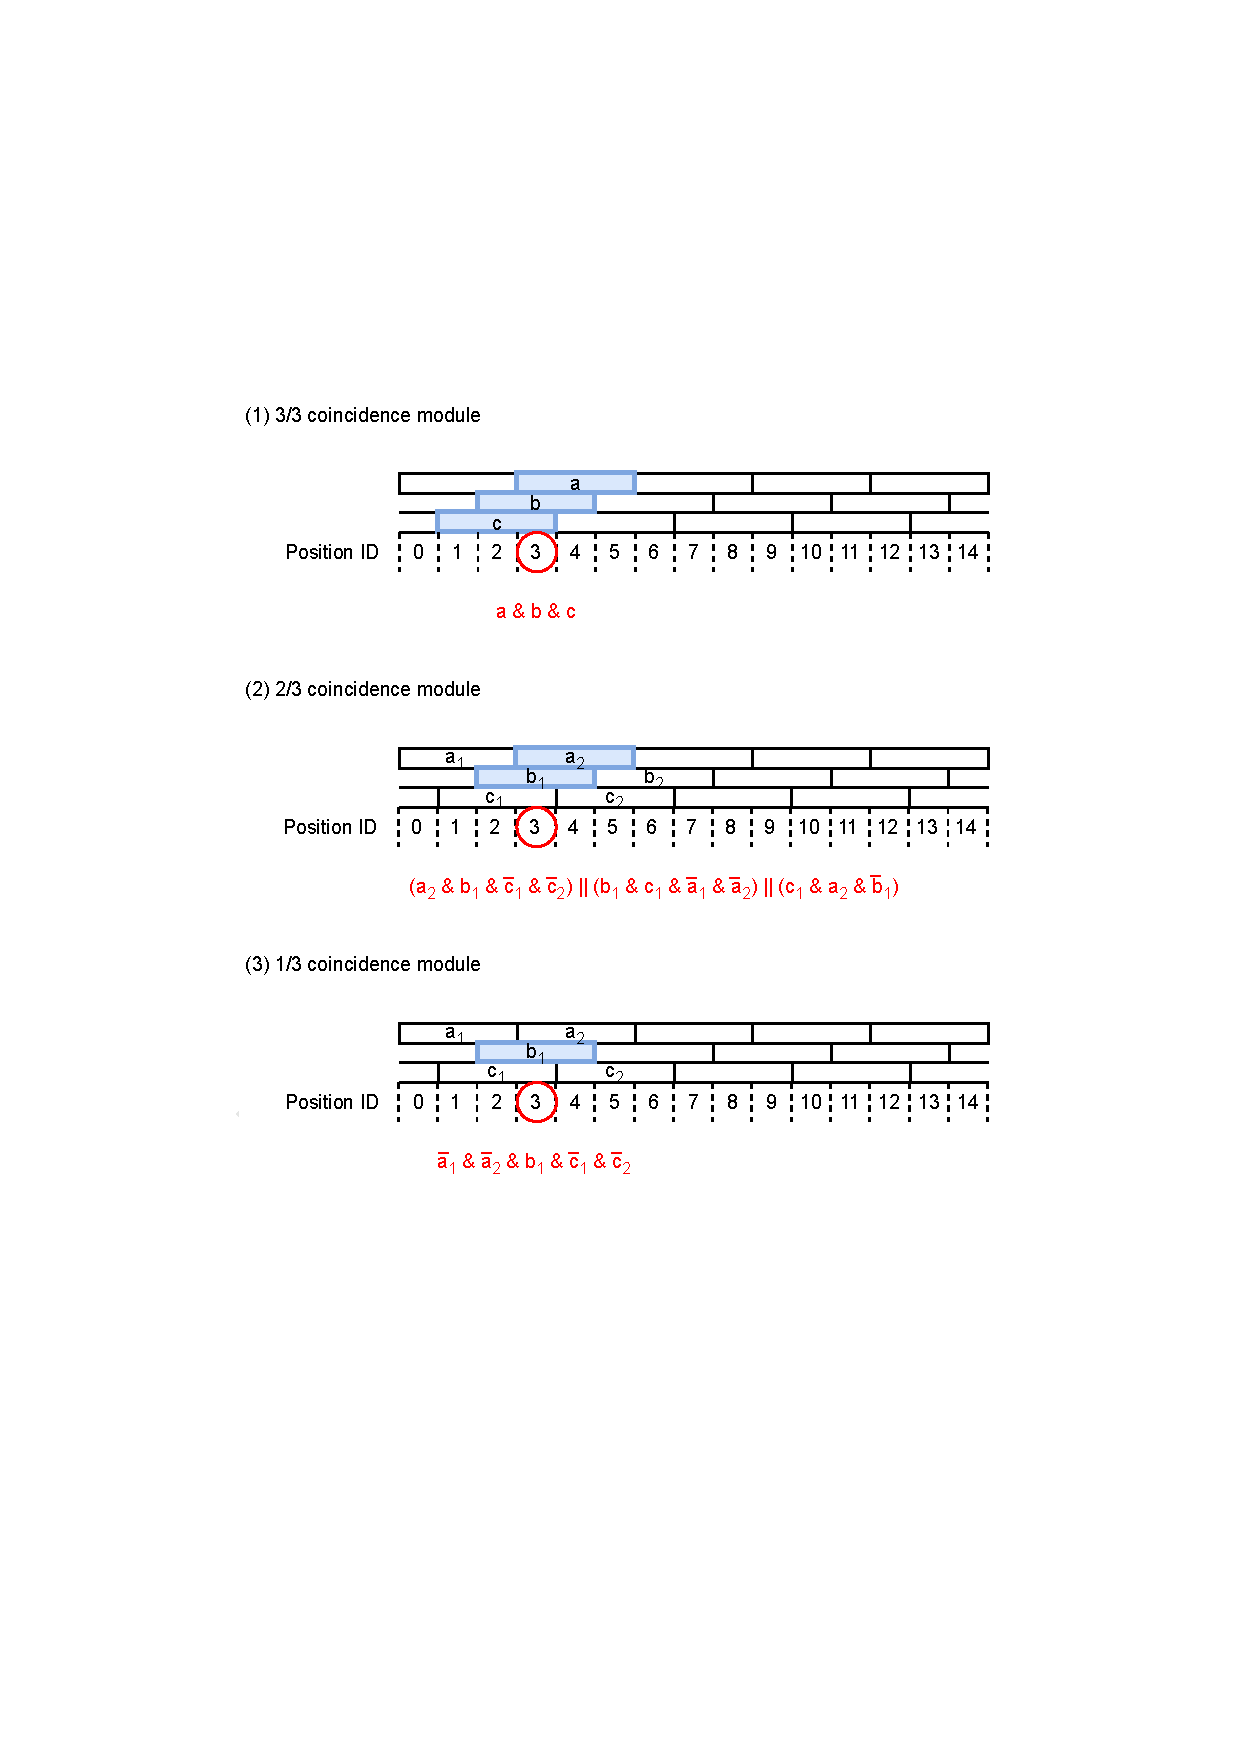
\includegraphics[width=16cm]{fig/SL/StationCoin_wire.pdf}
    \caption[M1 tripletにおけるコインシデンスロジック]{M1 tripletにおけるコインシデンスロジック}
    \label{StationCoin_wire}
\end{figure}

M2、M3ステーションは2層で構成されているため、2/2コインシデンスと1/2コインシデンスが用意されており、それぞれのロジックは図\ref{StationCoin_doublet}のように実装される。
    
\begin{figure} 
\centering
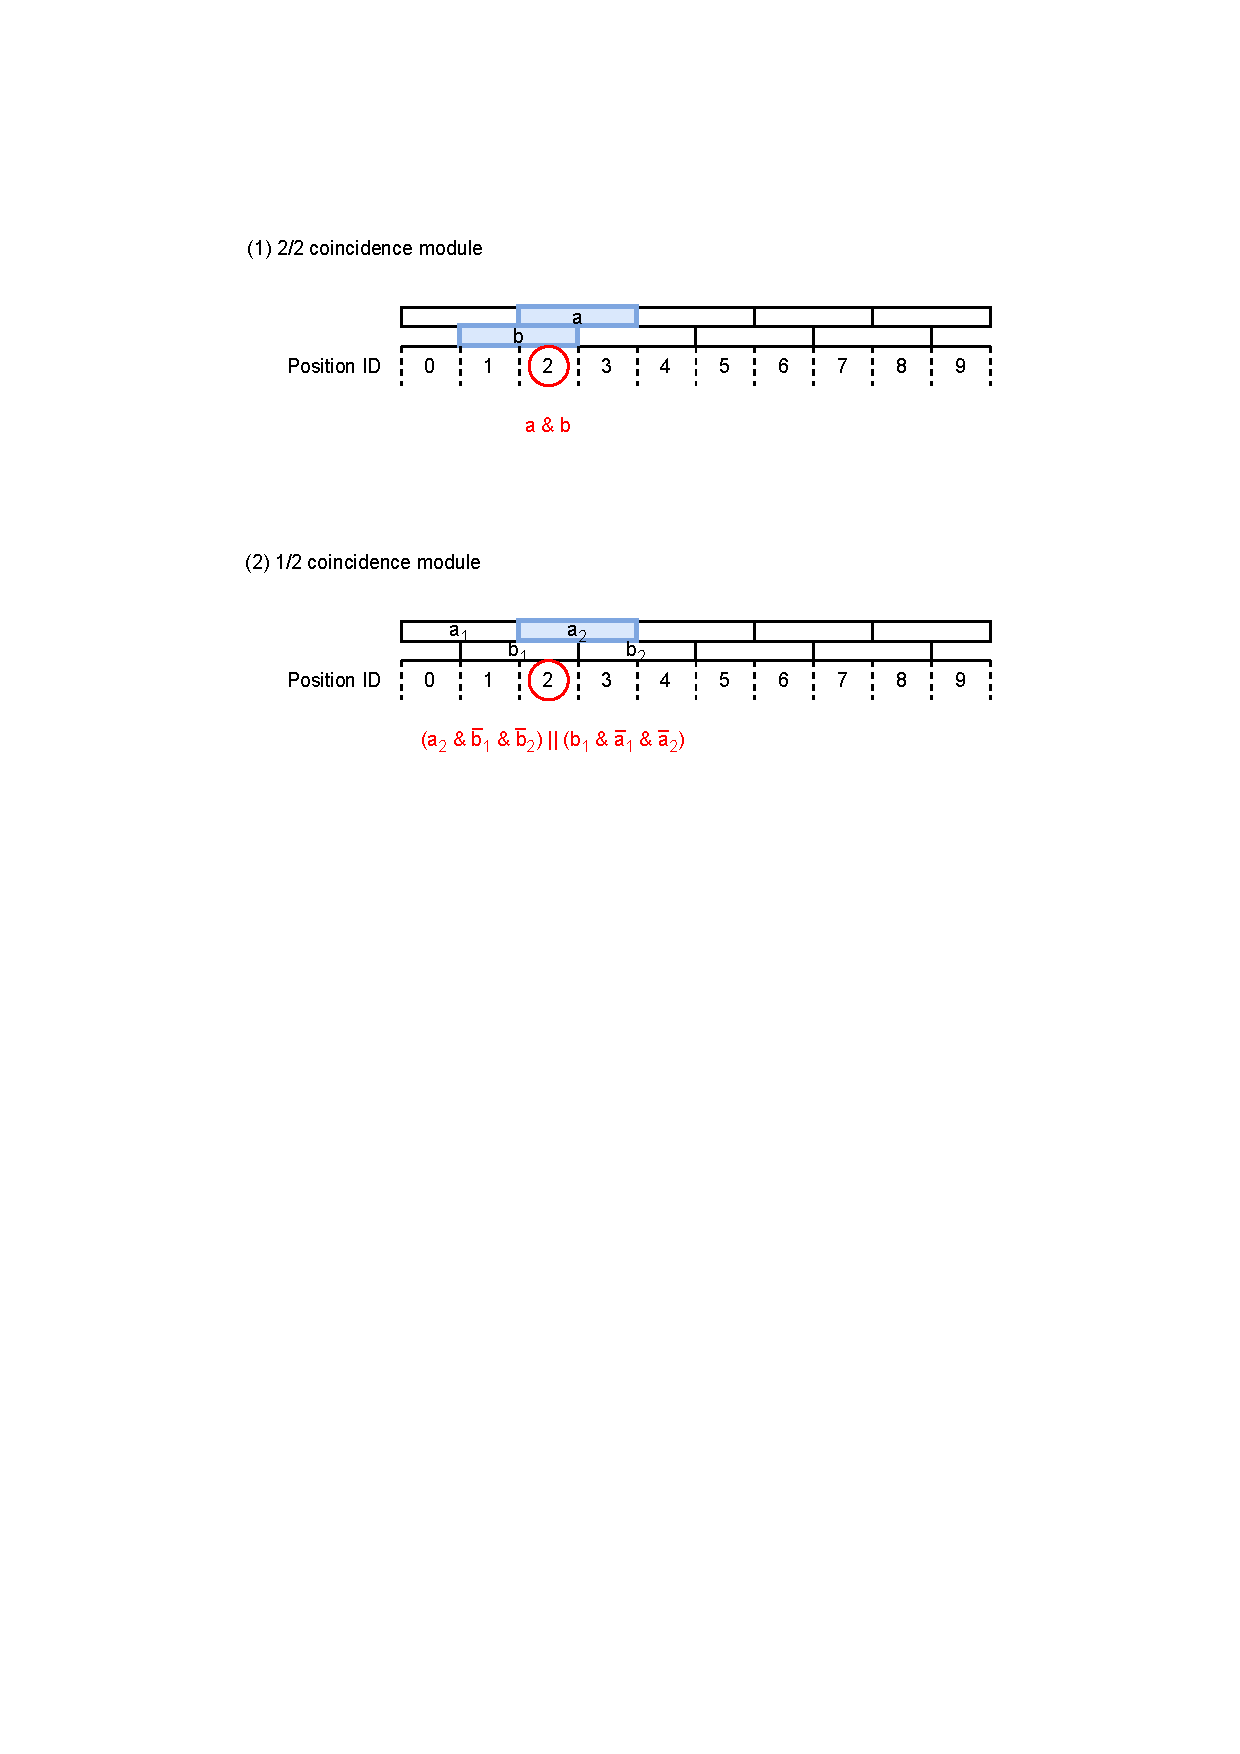
\includegraphics[width=16cm]{fig/SL/StationCoin_doublet.pdf}
\caption[M2・M3 ステーションにおけるコインシデンスロジック]{M2・M3 ステーションにおけるコインシデンスロジック}
\label{StationCoin_doublet}
\end{figure}

各コインシデンスロジックで、複数の代表点が出力された場合には各サブユニットごとに後段に送る代表点を選別する。M1、M2ステーションでは検出器がユニットの中心により近いものが2つ、M3ステーションでは$\eta$がより小さいものが1つ選ばれる。これらのロジックはより大きな\pt のミューオンを通すことを目的に、ソフトウェアでのシミュレーションなどを経て最適化されたものである。
% ステーションコインシデンスの最終的な出力は図\ref{}のテーブルのようにまとめらる。

\subsubsection*{Strip Station CoincidenceのHDL実装}
このモジュールの駆動クロックは、LHCバンチ交差クロックに同期した40 MHzクロックでレイテンシーは1クロックチック ( 25 ns )である。Strip Station Coincidenceおよび\ref{subsec:segment_reco}節で説明するStrip Segment ReconstructionもUnit、Subunit呼ばれる単位領域でトリガーセクターを分割して、Subunitごとに並列にコインシデンスロジックを走らせる。Strip では 1つのチェンバーを4分割するようユニットが定義される。エンドキャップ領域は5枚のチェンバーで構成されるため20 Unit、フォワード領域は1枚のチェンバーで構成されるため5 unit 存在する。図\ref{StationCoin_unit_strip}にユニットの構造を示す。1つのユニットはM1ステーションの40 代表点、M2ステーションの24代表点、M3ステーションの16代表点をカバーする。また、1つのユニットを2等分するようにしてSubunitが定義されている。

\begin{figure} 
    \centering
    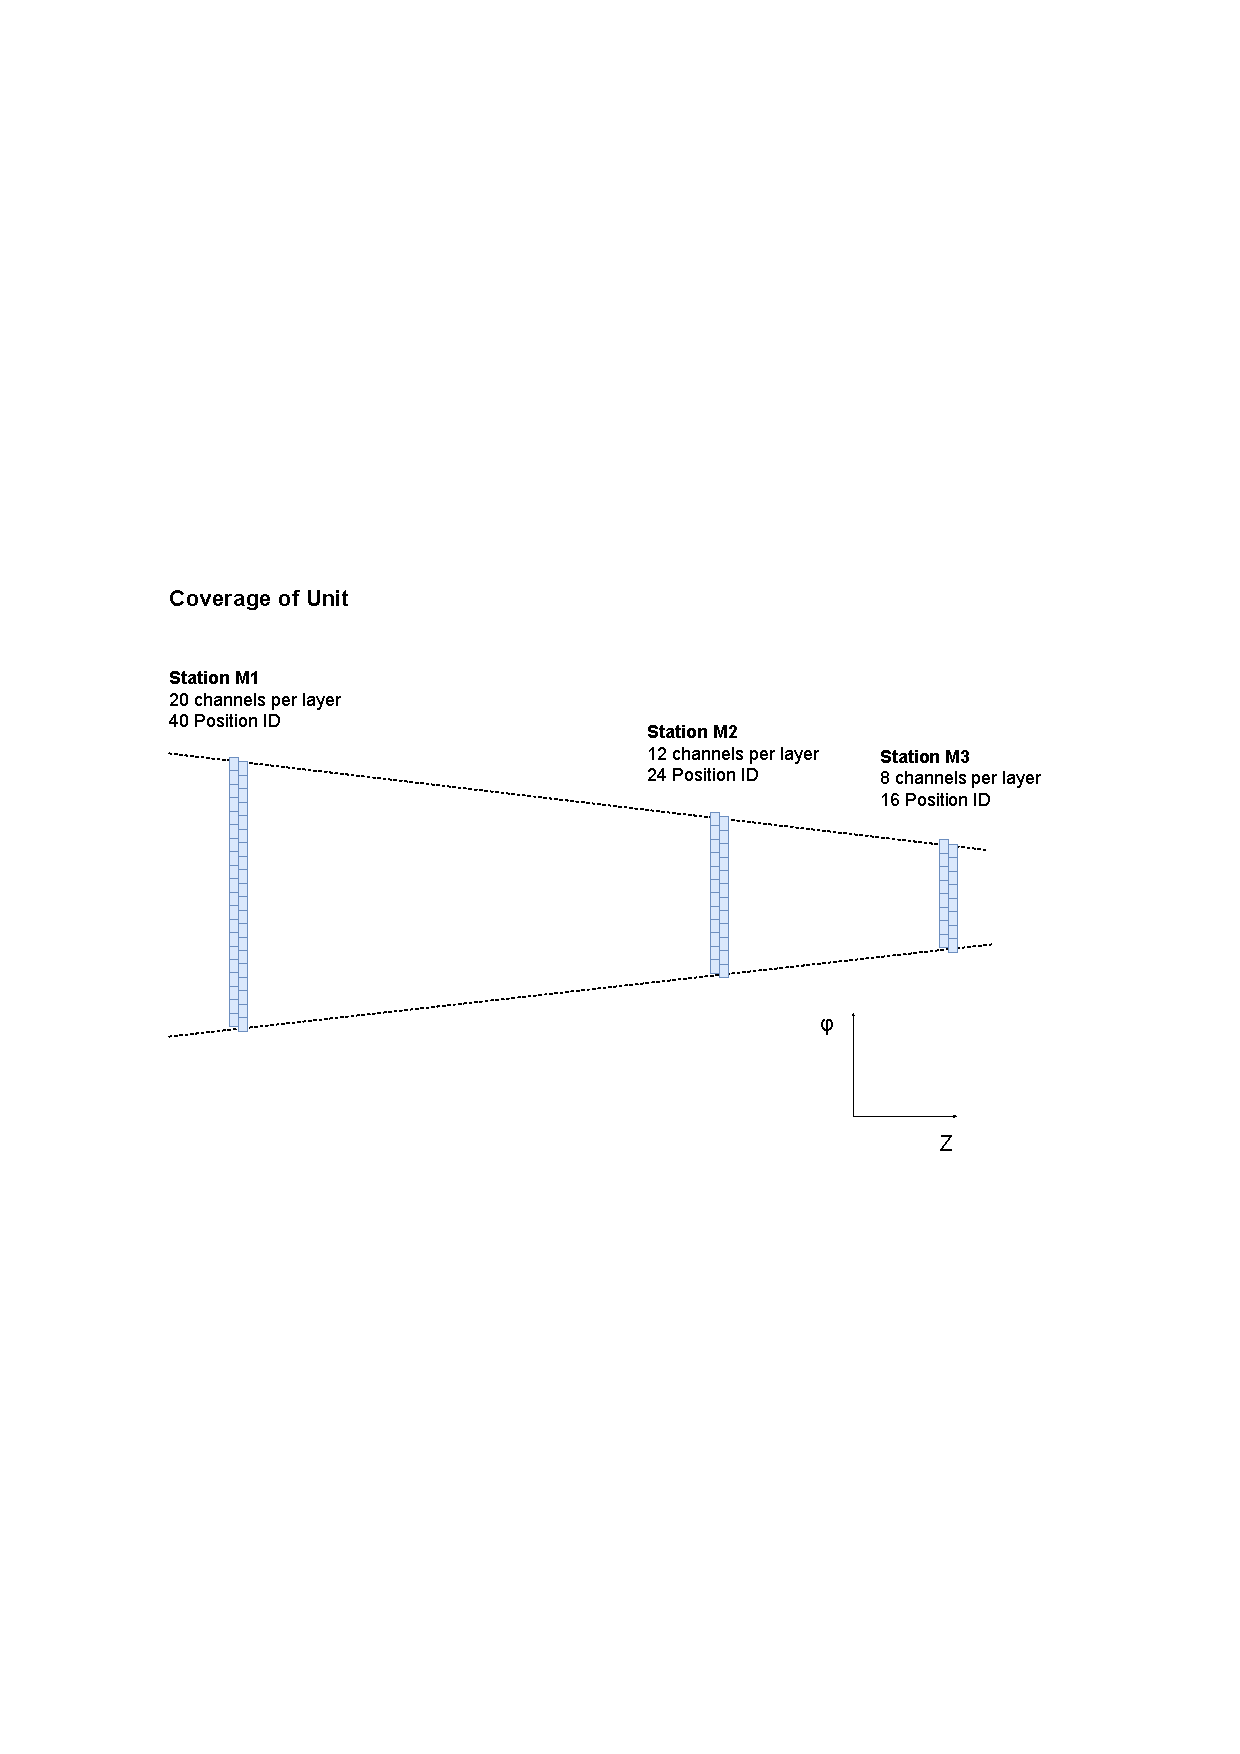
\includegraphics[width=16cm]{fig/SL/StationCoin_unit_strip.pdf}
    \caption[Strip Station Coincidence および Strip Segment Reconstruction におけるユニット]{Strip Station Coincidence および Strip Segment Reconstruction におけるユニット}
    \label{StationCoin_unit_strip}
\end{figure}

コインシデンスのロジックは基本的にワイヤーと同じで、M1、M2、M3ともに2層構造になっているためそれぞれ2/2、1/2ロジックが並列に走っている。
% 最終的な出力は図\ref{}のようにまとめられ、後段に送られる。


\subsection{Segment Reconstruction}
\label{subsec:segment_reco}
\subsubsection*{コンセプト}
Segment Reconstructionではステーションコインシデンスで取り出された、各ステーションの代表点の組み合わせから、無限運動量飛跡と実際の飛跡のなす角度 ($\Delta\theta$、$\Delta\phi$)を算出する。Segment Reconstructionの概念図を図\ref{Concept_segment}に示す。角度情報の概算には、パターンマッチングと呼ばれる手法を用いる。この手法ではあらかじめ、代表点の組み合わせとそこから計算される角度情報の対応関係をまとめたテーブル (パターンリスト、LUTともよぶ) を用意することで、複雑な計算をせずとも高速で角度情報を再構成する。

\begin{figure} 
\centering
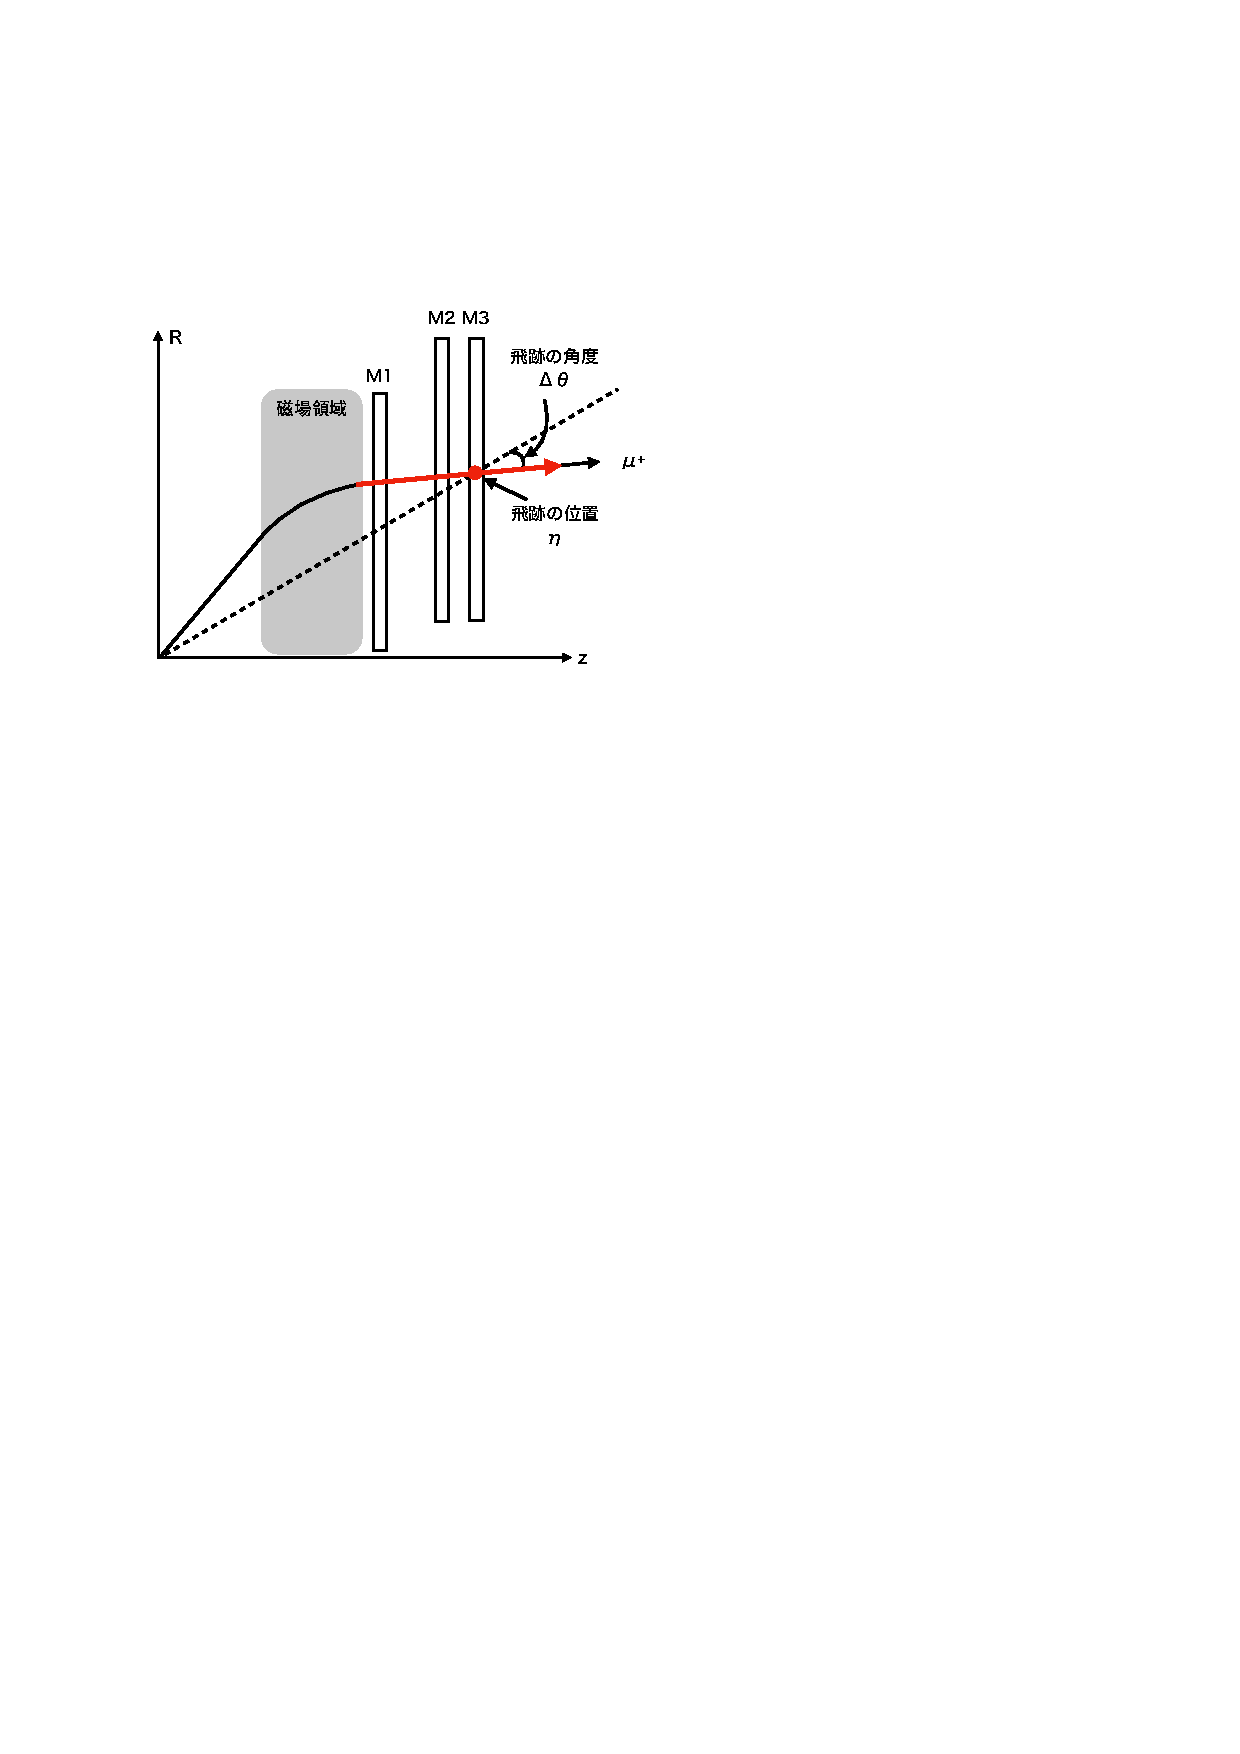
\includegraphics[width=16cm]{fig/SL/Concept_segment.pdf}
\caption[Segment Reconstructionのコンセプト]{$\eta$方向 (左) および$\phi$方向 (右) のパターンマッチングの概念図\cite{mt_mino}。黒い線が実際のミューオンの飛跡を表し、赤い線がTGCのヒットから再構成される飛跡を表す。黒い点線はM3ステーションの代表点と衝突点を結んだ、無限運動量飛跡を表し、再構成した飛跡と無限運動量飛跡との角度をパターンとして保存する。}
\label{Concept_segment}
\end{figure}

\subsubsection*{Wire Segment ReconstructionのHDL実装}
このモジュールの駆動クロックは、LHC クロックに同期した周波数 160 MHz のクロックであり、レイテンシは 12 クロックチック分 (75 ns) である。
Wire Segment Reconstructionではサブユニットごとに1つLUTが用意され、サブユニット内のM1、M2、M3代表点を組み合わせることでパターンマッチングを行う。最終的にはそれぞれのサブユニットから最大1つの飛跡情報を出力するため、SL全体では最大360の角度情報が出力される。Wire Segment Reconstructionの各サブユニット内でのロジックの概要を図\ref{SegReco_wire}に示す。各サブユニットはAddress Specifier・Segment Extractor・Segment Selector で構成される。以下でそれぞれのモジュールについて述べる。

\begin{figure} 
\centering
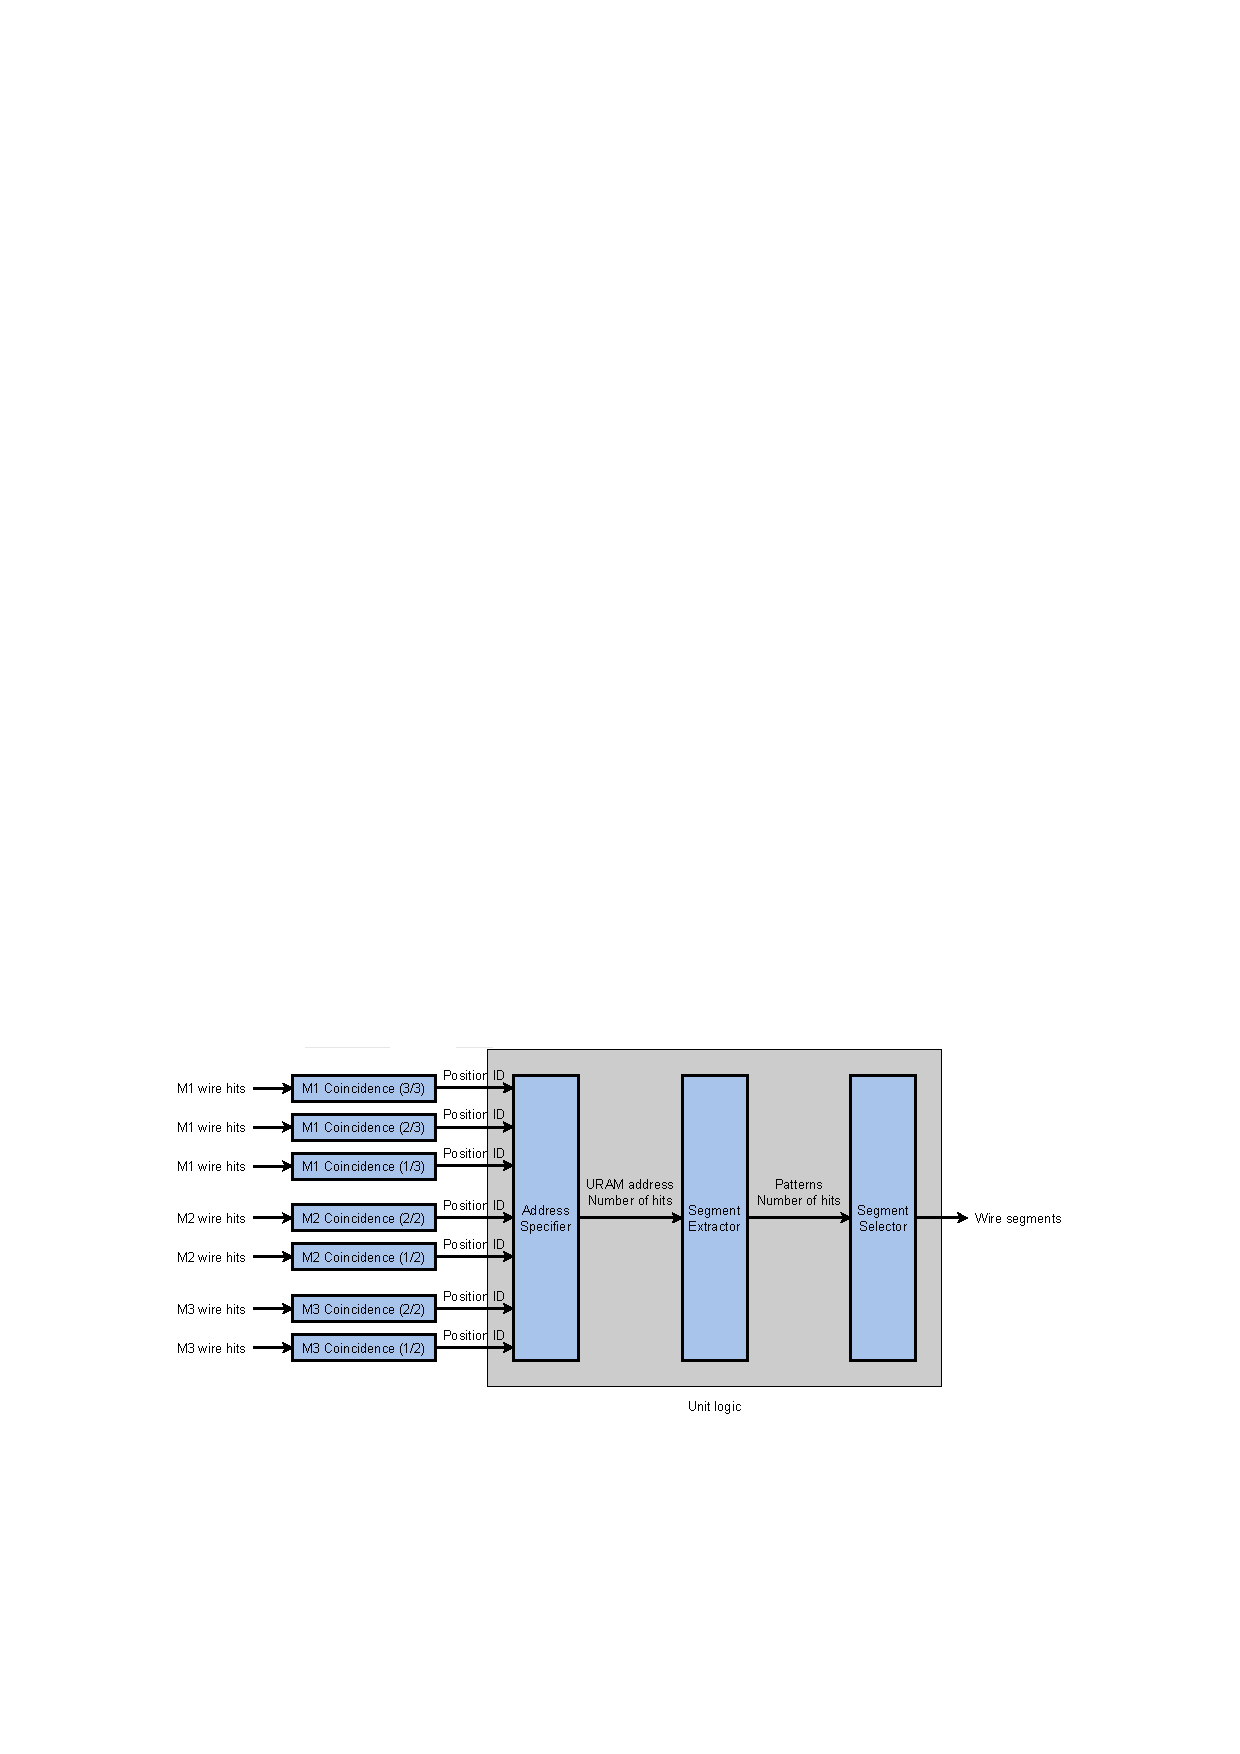
\includegraphics[width=16cm]{fig/SL/SegReco_wire.pdf}
\caption[Wire Segment Reconstructionのブロックダイアグラム]{Wire Segment Reconstructionのブロックダイアグラム\cite{SLPDR}}
\label{SegReco_wire}
\end{figure}

\subsubsection*{Address Specifier}
Wire Station Coincidenceで得られた各ステーションの代表点を組み合わせて、LUT にアクセスするためのアドレスを作成する。ステーションコインシデンスからは最大M1 個 6個、M2 4個、M3 2個の代表点が送られるため、最大 6 x 4 x 2 = 48 パターンの組み合わせが取られるが、この中から8つのパターンを選抜してSegment Extractorへ送る。パターンを選択する際にはマッチレイヤーが多いもの優先する。具体的に優先順位を定めたテーブルを表\ref{tab:StationCoin_wire}に示す。より上位にリストされているコインシデンスパターンが優先して送られる。また同じコインシデンスパターンが複数存在する場合には、$\eta$がより小さいものが選ばれる。この選び方もソフトウェアシミュレーションによる先行研究に基づいており、こうすることでより高い角度分解能で飛跡を再構成できることがわかっている。なお、同表中のFractionの値はミューオンがガスレイヤーを通過した時にヒットを残す確率を94 \%と仮定して算出したものである。

\begin{table}[h]
    \centering
    \caption{Wire Station Coincidenceにおけるコインシデンスパターン}
    \label{tab:StationCoin_wire}
    \begin{tabular}{|cc|c|}
    \hline
    \multicolumn{1}{|c|}{\multirow{2}{*}{Coincidence Pattern}} & Hit Pattern & \multirow{2}{*}{Faraction} \\ \cline{2-2}
    \multicolumn{1}{|c|}{}                                     & M1 M2 M3    &                            \\ \hline\hline
    \multicolumn{1}{|c|}{7/7}                                  & 3/3 2/2 2/2 & 0.649                      \\ \hline
    \multicolumn{1}{|c|}{6/7A}                                 & 2/3 2/2 2/2 & 0.124                      \\ \hline
    \multicolumn{1}{|c|}{6/7B}                                 & 3/3 1/2 2/2 & 0.083                      \\ \hline
    \multicolumn{1}{|c|}{6/7C}                        & 3/3 2/2 1/2 & 0.083                      \\ \hline
    \multicolumn{1}{|c|}{5/7A}                                 & 2/3 1/2 2/2 & 0.016                      \\ \hline
    \multicolumn{1}{|c|}{5/7B}                                 & 1/3 2/2 1/2 & 0.016                      \\ \hline
    \multicolumn{1}{|c|}{5/7C}                                 & 3/3 1/2 1/2 & 0.011                      \\ \hline
    \multicolumn{1}{|c|}{5/7D}                                 & 1/3 2/2 2/2 & 0.008                      \\ \hline\hline
    \multicolumn{2}{|c|}{Total}                                              & 0.988                      \\ \hline
    \end{tabular}
\end{table}

\subsubsection*{Segment Extractor}
Wire Segment Reconstructionで利用されるLUTはFPGAのURAM上に格納される。Segment ExtractorではAddress Specifierで作られたアドレスをもとに、URAMにアクセスし、対応するデータ (Wire Segment) を出力する。Wire Segmentのデータフォーマットを表\ref{tab:WireSegment}に示す。URAMはdual portで設計されており、1つのサブユニットが2ポート利用する。そのため1つのサブユニットは40 MHz クロック 1チックの間で 8つのデータを処理する。

\begin{table}[h]
    \centering
    \caption{Wire Segmentのフォーマット}
    \label{tab:WireSegment}
    \begin{tabular}{|c|c|}
    \hline
    \# of bits & Name                                                                       \\ \hline\hline
    1          & Flag of successful reconstruction                                          \\ \hline
    2          & Number of the stations with hits used for coincidence                      \\ \hline
    8          & Angle difference $\Delta\theta$ between the segment and the vector from IP \\ \hline
    12         & Global $\eta$ position of the segment                                      \\ \hline
    \end{tabular}
\end{table}

\subsubsection*{Segment Selector}
Segment Extractorから送られる最大8つのWire Segment から マッチレイヤーの多さを基準に最大1つ選択して、Wire Strip Coincidence へと送信する。マッチレイヤーも同じものが複数ある場合には$\Delta\theta$がより小さいものを選ぶ。

\subsection*{Strip Segment Reconstruction}
このモジュールの駆動クロックは、LHC クロックに同期した周波数 240 MHz のクロックであり、レイテンシーは 21 クロックチック分 (87.5 ns) である。
Strip Segment Reconstructionではサブユニットごとに1つLUTが用意され、サブユニット内の代表点を組み合わせることでパターンマッチングを行う。最終的にはユニット内の2つのサブユニット合わせて、1つの角度情報が出力される。SL全体では最大45の飛跡情報が出力される。Strip Segment Reconstructionの各サブユニット内でのロジックの概要を図\ref{SegReco_strip}に示す。各サブユニットはAddress Specifier・Segment Extractor・Segment Selector で構成される。以下でそれぞれのモジュールについて述べる。

\begin{figure} 
\centering
\includegraphics[width=16cm]{fig/SL/SegReco_strip.pdf}
\caption[Strip Segment Reconstruction のブロックダイアグラム]{Strip Segment Reconstruction のブロックダイアグラム}
\label{SegReco_strip}
\end{figure}

\subsubsection*{Address Specifier}
Strip Station Coincidenceで得られた各ステーションの代表点を組み合わせて、LUT にアクセスするためのアドレスを作成する。ステーションコインシデンスからは最大M1 個 4個、M2 4個、M3 2個の代表点が送られるため  4 x 4 x 2 = 32 パターンの組み合わせが取られうるが、この中から6つのパターンを選抜してSegment Extractorへ送る。パターンを選択する際にはワイヤーのロジックと同様にマッチレイヤーが多いもの優先する。具体的に優先順位を定めたテーブルを表\ref{tab:SegmentReco_strip}に示す。

\begin{table}[]
    \centering
    \caption{Strip Segment Reconstructionにおけるwire segmentのデータフォーマット}
    \label{tab:SegmentReco_strip}
    \begin{tabular}{|cc|}
    \hline
    \multicolumn{1}{|c|}{\multirow{2}{*}{Coincidence Pattern}} & Hit Pattern \\ \cline{2-2} 
    \multicolumn{1}{|c|}{}                                     & M1 M2 M3    \\ \hline\hline
    \multicolumn{1}{|c|}{6/6}                                  & 2/2 2/2 2/2 \\ \hline
    \multicolumn{1}{|c|}{5/6A}                                 & 2/2 1/2 2/2 \\ \hline
    \multicolumn{1}{|c|}{5/6B}                                 & 1/2 2/2 2/2 \\ \hline
    \multicolumn{1}{|c|}{5/6C}                                 & 2/2 2/2 1/2 \\ \hline
    \multicolumn{1}{|c|}{4/6A}                                 & 1/2 1/2 2/2 \\ \hline
    \multicolumn{1}{|c|}{4/6B}                                 & 2/2 1/2 1/2 \\ \hline
    \multicolumn{1}{|c|}{4/6C}                                 & 1/2 2/2 1/2 \\ \hline\hline
    \multicolumn{2}{|c|}{Total}                                              \\ \hline
    \end{tabular}
\end{table}

\subsubsection*{Segment Extractor}
Strip Segment Reconstructionで利用されるLUTはFPGAのURAM上に格納される。Segment ExtractorではAddress Specifierで作られたアドレスをもとに、URAMにアクセスし、対応するデータ (Strip Segment) を出力する。Strip Segmentのデータフォーマットを表\ref{tab:StripSegment}に示す。URAMはdual portで設計されており、2つのサブユニットが1ポートずつ利用する。そのため1つのサブユニットは、40 MHzクロック 1チックの間に6つのデータを処理する。

\begin{table}[]
    \centering
    \caption{Strip Segmentのフォーマット}
    \label{tab:StripSegment}
    \begin{tabular}{|c|c|}
    \hline
    \# of bits & Name                                                                     \\ \hline\hline
    2          & Number of the stations with hits used for coincidence                    \\ \hline
    6          & Local $\phi$ position in the chamber                                     \\ \hline
    9          & Angle difference $\Delta\phi$ between the segment and the vector from IP \\ \hline
    \end{tabular}
\end{table}

\subsubsection*{Segment Selector}
Segment Extractorから送られる最大6つのStrip Segment から マッチレイヤーの多さを基準にユニットごとに最大1 Segment 選択して、Wire Strip Coincidence へと送信する。マッチレイヤーも同じものが複数ある場合には$\Delta\phi$がより小さいものを選ぶ。

\subsection{Wire-Strip Coincidence}
\subsubsection*{コンセプト}
Wire Strip CoincidenceではWire Segment Reconstructionで算出した$\Delta\eta$とStrip Segment Reconstructionで算出した$\Delta\phi$を組み合わせることで、横方向運動量\pt を概算する。\pt の計算もCoincidence Windowと呼ばれるLUTを用いて行う。Coincidence Windowの例を図\ref{Concept_WS}に示す。

\begin{figure} 
\centering
\includegraphics[width=16cm]{fig/SL/Concept_WS.pdf}
\caption[Wire Strip CoincidenceにおけるCoincidence Windowの例]{Wire Strip CoincidenceにおけるCoincidence Windowの例\cite{SLPDR}。本番運用時には$p_\mathrm{T}$は4 bit、16段階で出力する予定であるが、現状はテストのため5 GeV、10 GeV、15 GeV、20 GeVの4段階で出力している。}
\label{Concept_WS}
\end{figure}

\subsubsection*{Wire Strip CoincidenceのHDL実装}
駆動クロックはLHCバンチ交差クロックに同期した160 MHzクロック。レイテンシーは6クロックチック分 (37.5 ns)である。
Wire Strip CoincidenceではReginoと呼ばれる単位領域を新たに設定し、Regionごとに並列にコインシデンスを行う。Regionは後段のInner Coincidenceのコインシデンスをとる単位に合わせて定義されている。Wire Strip CoincidenceにおけるRegionの定義を図\ref{WS_region}に示す。エンドキャップ領域は|$\eta$| < 1.3 領域では 8 Unit、|$\eta$| < 1.3 領域では32 Unit という異なる大きさの Regionを定義し、それぞれの領域を22分割、13分割する。フォワード領域は32 Unit Regionで8分割する。

\begin{figure} 
\centering
\includegraphics[width=16cm]{fig/SL/WS_region.pdf}
\caption[Wire Strip Coincidence以降のRegionの分割]{Wire Strip Coincidence以降のRegionの分割\cite{mt_kawamoto}。Endcap 領域では 8 Unit Regionと32 Unit Regionという2種類の領域を用意する。}
\label{WS_region}
\end{figure}

図\ref{WS_Concept}に1つのUnitの構造を示す。8 Unit Regionはトリガーセクターの全て$\phi$領域に当たるストリップの4 Unitからのstrip segmentと ワイヤーの2 Subunitからのwire segmentを組み合わせて、最大1つの飛跡候補を出力する。32 Unit Regionはストリップの 4 Unitからのstrip segmentと、ワイヤーの 8 Subunitからのwire segmentを組み合わせて、最大4つの候補を出力する。SL全体では最大180この飛跡候補が出力される。

\begin{figure} 
\centering
\includegraphics[width=16cm]{fig/SL/WS_Concept.pdf}
\caption[]{8 Unit Region、32 Unit Regionにおけるコインシデンスの概要\cite{mt_kawamoto}}
\label{WS_Concept}
\end{figure}

Wire Strip Coincidenceの各Unit内でのロジックの概要を図\ref{}に示す。各ユニットは\pt Calculator、Wire Position Corrector、Block Selectorで構成される。以下でそれぞれのモジュールについて述べる。

\begin{figure} 
\centering
\includegraphics[width=16cm]{fig/SL/WS_logic.pdf}
\caption[Wire Strip Coincidence ファームウェアの概要]{Wire Strip Coincidence ファームウェアの概要\cite{mt_kawamoto}}
\label{WS_logic}
\end{figure}

\subsubsection*{\pt Calculator}
\pt Calculatorはwire segmentに含まれる8 bitの$\Delta\theta$及びstrip segmentに含まれる9 bitの$\Delta\phi$から、Coincidence Windowにアクセスするためのアドレスを作成し、Coincidence Windowに格納された4 bitの\pt を出力する。1つの\pt Calculatorは1つのwire segmentと4つのstrip segmentを組み合わせ、全ての組み合わせに対して\pt を出力する。Coincidence WindowはFPGAのdual BRAM上に格納されているため、この処理は2クロックチックで完了する。

\subsubsection*{Wire Position Corrector}
wire segment や strip segmentに含まれる位置情報は代表点のIDだが、Inner Coincidenceでは位置情報として$\eta$を利用する。また、代表点IDと$\eta$の関係はUnit Regionごとにばらつきがあることが知られており\footnote{wireの代表点が$\eta$に対して均一に並んでいないことと、$\phi$位置ごとでも代表点と$\eta$の対応関係は異なることによる}、全てのUnitで共通に変換できる訳ではない。そこでwireとstripの代表点と$\eta$位置の対応関係をパターンリストとして保存し、Unitごとに$\eta$の再構成を行う。これを担当するモジュールWire Position Correctorと呼ぶ。

\subsubsection*{Block Selector}
Block Selectorはワイヤーとストリップの組み合わせで生じる複数のミューオン飛跡候補から、後段に送る飛跡候補を選択する。飛跡の選抜はマッチした層数の多さを基準に行い、マッチした層数も同じ場合は角度がより小さいものを選択する。8 Unit Regionでは4つのストリップ飛跡と2つのワイヤー飛跡から再構成される計8個の飛跡候補から、最大1つの候補を絞り込む。32 Unit Regionでは4つのストリップ飛跡と8つのワイヤー飛跡の組み合わせからなる32個の飛跡候補から最大4つの候補を選ぶ。この時、2つは$\Delta\theta$が正の方向に曲げられたもの,もう2つは負に曲げられたものが選ばれるように設計する。これはJ/$\psi$ 粒子などから生じる、2つの異符号ミューオンを積極的に取れるようにするための実装である。
Wire Strip CoincidenceからInner Coincidenceに送られる飛跡情報のフォーマットを図\ref{tab:WS}に示す。本研究ではChannel MappingからWire Strip CoincidenceまでのトリガーロジックをTGC BW Coincidenceと呼ぶ。

\begin{table}[]
    \centering
    \caption{Wire Strip Coincidenceにおける飛跡候補のデータフォーマット}
    \label{tab:WS}
    \begin{tabular}{|c|c|}
    \hline
    \# of bits & Name                                                                                        \\ \hline\hline
    1          & Valid flag which means this region receive the more than one strip segment and wire segment \\ \hline
    4          & $p_{\mathrm{T}}$ threshold reconstructed using Coincidence Window                           \\ \hline
    8          & Local $\eta$ position in the unit                                                           \\ \hline
    3          & Unit ID                                                                                     \\ \hline
    7          & Angle difference $\Delta\eta$ between the segment and the vector from IP                    \\ \hline
    2          & Number of stations with the hits used for wire segment reconstruction                       \\ \hline
    4          & Angle difference $\Delta\phi$ between the segment and the vector from IP                    \\ \hline
    2          & Number of stations with the hits used for strip segment reconstruction                      \\ \hline
    \end{tabular}
\end{table}

\subsection{Inner Coincidence}
\subsubsection*{コンセプト}
nner CoincidenceではTGC BW コインシデンスで再構成された飛跡候補と磁場領域内部の検出器 (NSW、RPC BIS78、TGC EI、Tile カロリメーター)でコインシデンスととることで、衝突点に由来しないフェイクトリガーの削減と\pt 分解能の向上を図る。磁場内部に位置する検出器はそれぞれ異なる特徴を持っているため、コインシデンスをとる検出器ごとに独立したロジックが用意されている。ここでは具体例としてNSWとのコインシデンスロジックについて説明する。

図\ref{Concept_NSW}にNSWとのコインシデンスアルゴリズムの概要を示す。衝突点から飛来するミューオンはNSWにヒットを残した後エンドキャップトロイド磁場により主に$\eta$方向に曲げられ、TGCにヒットを残す。そのためTGC BW コインシデンスで再構成された$\eta$位置($\eta_{\mathrm{TGC}}$)とNSWで再構成された$\eta$位置($\eta_{\mathrm{NSW}}$)差が\pt と相関をもつ。この差$d\eta$を式(\ref{eq:deta})に定義する。

\begin{figure} 
\centering
\includegraphics[width=16cm]{fig/SL/Concept_NSW.pdf}
\caption[NSW を用いたコインシデンスロジックの概要]{NSW を用いたコインシデンスロジックの概要\cite{mt_akatsuka}}
\label{Concept_NSW}
\end{figure}

\begin{equation}
    d\eta = \eta_{\mathrm{TGC}} - \eta_{\mathrm{NSW}}
    \label{eq:deta}
\end{equation}

しかし、衝突点から飛来するミューオンは検出器内部の物質 ( 主に物質量の大きいカロリーメータ )と多重散乱を起こすことがあり、この場合では$d\eta$のみでは\pt が高いものと低いものを見分けることができない。そこで、ミューオンがNSWに入射した角度 ($\Delta\theta_{\mathrm{NSW}}$) を分別変数として追加することで、より正確に\pt 判定を行うことができる。この計算にも$d\eta$、($\Delta\theta_{\mathrm{NSW}}$) を入力、\pt を出力としたCoincidence Windowが利用される。

\subsubsection*{Inner CoincidenceのHDL実装}
このモジュールの駆動クロックは、LHC クロックに同期した周波数 160 MHz のクロックであり、レイテンシーは 7 クロックチック分 (43.75 ns) である。

Inner CoincidenceもRegionを1単位として並列に処理が行われる。$\eta$位置ごとにどの検出器とコインシデンスをとるかが決められており、|$\eta$| < 1.3 の領域では主にRPC、EI、Tileカロリメーターと、|$\eta$| > 1.3の領域では主にNSWとコインシデンスをとる。8 Unit RegionはWire Strip Coincidenceから1つの飛跡候補を受け取り、コインシデンスをとった後1候補を出力する。32 Unit RegionはWire Strip Coincidenceから4つの飛跡候補を受け取り、2つまで候補を絞って出力する。その結果SL全体では最大112候補を出力する。

Inner Coincidenceの各Unit 内でのロジックの概要を図\ref{Inner_logic}に示す。各ユニットはDecoder、Coincidence、Which Innerで構成される。以下に例としてNSWとのコインシデンスをとるRegionについて説明する。

\begin{figure} 
\centering
\includegraphics[width=16cm]{fig/SL/Inner_integrate.png}
\caption[Inner Coincidenceの概要]{Inner Coincidenceの概要\cite{mt_kobayashi}}
\label{Inner_logic}
\end{figure}

\begin{itemize}
    \item Decoder\\
    1つのSLはNSWで再構成された飛跡を最大16個受け取る。この中からTGC BW コインシデンスで再構成された飛跡候補と組み合わせる4候補を選ぶのがDecoderである。ここでは\pt が大きいミューオンの検出効率を高く保つため、|$d\eta$|が小さいものを優先的に選別する。
    \item NSW Coincidence\\
    TGC BW の1つの飛跡候補とNSWの4つの飛跡候補でコインシデンスをとる。Coincidence WindowはFPGAのURAMに格納されており、8 bitの$d\eta$情報と4 bitの$\Delta\theta$を入力、4 bitの\pt を出力とする。計算された飛跡のうち、\pt が最大の候補が保存され40 MHzごとに出力される。
    \item Which Inner\\
    Which Inner モジュールは複数の検出器とのコインシデンスロジックが並列に走る|$\eta$| < 1.3の領域において、どの検出器とのコインシデンス結果を最終出力とするかを決定する。
\end{itemize}

Inner CoincidenceからTrack Selectorに送られる飛跡候補のデータフォーマットを表 \ref{tab:InnerCoin} に示す。

\begin{table}[]
    \centering
    \caption{Inner Coincidenceにおける飛跡候補のデータフォーマット}
    \label{tab:InnerCoin}
    \begin{tabular}{|c|c|c|}
    \hline
    \# of bits & Name                             & Comment                                                                \\ \hline\hline
    14         & TGC $\eta$                       & $\eta$ in global candidate at the pivot plane of TGC                   \\ \hline
    9          & TGC $\phi$                       & $\phi$ in global candidate at the pivot plane of TGC                   \\ \hline
    8          & TGC \textbackslash{}pt           & TGC transverse momentum                                                \\ \hline
    4          & TGC \textbackslash{}pt threshold & TGChighest \textbackslash{}pt thresholdsatisfied                       \\ \hline
    1          & TGC charge                       & TGC TC charge                                                          \\ \hline
    3          & Coincidence type                 & Identifier of coincidence type                                         \\ \hline
    14         & MDT $\eta$                       & $\eta$ coordinate of the MDT segment position of the innermost station \\ \hline
    8          & MDT \textbackslash{}pt           & MDT transverse momentum                                                \\ \hline
    4          & MDT \textbackslash{}pt threshold & MDThighesttransversemomentumthresholdsatisfied                         \\ \hline
    1          & MDT charge                       & MDT charge                                                             \\ \hline
    4          & MDT Processing Flag              & Type of reconstructed muon                                             \\ \hline
    2          & \# of segments                   & Number of MDT segments associated to the muon                          \\ \hline
    3          & Segment quality flag             & Quality of each segment                                                \\ \hline
    49         & Reserved                         &                                                                        \\ \hline
    \end{tabular}
\end{table}

\subsection{Track Selector}
\subsubsection*{コンセプト}
Track SelectorはInner Coincidenceから出力される最大112個のミューオン飛跡候補からMUCTPIに送る6候補を選ぶ。このときInner Coincidenceで判定された\pt が高いものを優先的に選択する。

\subsubsection*{Track SelectorのHDL実装}
モジュールの駆動クロックはLHCクロックに同期した周波数160 MHzのクロックであり、レイテンシ-は5クロックチック (31.25 ns)である。
概要を図\ref{TrackSelector_overview}に示す。候補選別回路は4 bitの\pt が大きい順に候補を並び替えるソーティングロジックとして実装される。特にBatcherの奇遇マージソート法\cite{Batcher}という、並列処理のもとで高速でソーティングを行うことができる手法が採用された。Track Selectorは16個の8-key sorting network、と15個の16-key merging networkで構成され、インプットが128、アウトプットが8のソーティングロジックとなっている。8-key soting networkおよび16-key merging networkの概要を図\ref{Sortiing_8key}、\ref{Sorting_16}に示す。これらの図の横線はワイヤーを示し、縦軸がコンパレーターを表す。左から右に1つの飛跡候補同士の比較が行われ、それの集合体としてロジックが実装される。


\begin{figure} 
    \centering
    \includegraphics[width=16cm]{fig/SL/TrackSelector_overview.pdf}
    \caption[Track Selector の概要]{Track Selector の概要}
    \label{TrackSelector_overview}  
\end{figure}
    

\begin{figure} 
\centering
\includegraphics[width=16cm]{fig/SL/Sortiing_8key.pdf}
\caption[8-key sorting network の概要]{8-key sorting network の概要}
\label{Sortiing_8key}
\end{figure}

\begin{figure} 
\centering
\includegraphics[width=16cm]{fig/SL/Sorting_16.pdf}
\caption[16-key merging network の概要]{16-key merging network の概要}
\label{Sorting_16}
\end{figure}


\newpage
\section{Inner Coincidenceの統合}
\label{sec_TriggerIntegration}
2章で述べたように、SL FPGAの中でトリガーロジックは図\ref{}のように統合される。
PS board とのインターフェイスが実装されるSLR0・2・3には、TGC BW Coincidenceが実装される。トリガーセクターごとにSLRが分けられ、SLR0にEndcap $\phi\,0$、SLR2にEndcap $\phi\,1$、SLR3にForwardのロジックが配置される。磁場内部の検出器やMUCTPIとのインターフェイスはSLR1に実装され、ここにはInner Coincidence、Track Selectorが配置される。
高輝度LHC-ATLAS実験に向けたトリガー開発は、これまでに各モジュールのHDL実装が完了し、Segment Reconstructionまでの統合が完了している。

本研究では引き続きWire Strip Coincidence、Inner Coincidence、Track Selectorの統合を進め、一連のトリガーロジックの統合を完了させる。以下にそれぞれの実装について述べる。

\subsection{Wire Strip Coincidenceの統合}
Wire Strip Coincidenceを統合ファームウェアに組み込むため、前段のWire Segment Reconstruction、Strip Segment Reconstructionの出力を配線した他、モジュール内に存在する2種類のLUTをコンフィギュレーションするパスを接続した。
Wire Strip Coincidenceモジュールに接続した各信号線を表\ref{tab:WS_integrate}にまとめる。

\begin{table}[]
    \centering
    \caption{Wire Strip Coincidenceにおける信号線}
    \label{tab:WS_integrate}
    \begin{tabular}{|c|c|}
    \hline
    接続するモジュール                               & 信号線 ( bit幅 )                                                                                                    \\ \hline
    Wire Segment Reconstruction             & \begin{tabular}[c]{@{}c@{}}Wire Segment ( EC : 148 subunit x 20 bit, \\ FW : 64 subunit x 20 bit )\end{tabular} \\ \hline\hline
    Strip Segment Reconstruction            & Strip Segment ( EC :  20 unit x 17bit, FW : 5 unit x 17 bit)                                                    \\ \hline
    LUT Manager for \textbackslash{}pt LUT  & Address + Data  (EC : 35 region x 18 bit、FW : 8 unit x 18 bit )                                                 \\ \hline
    LUT Manager for \textbackslash{}eta LUT & Address + Data (EC : 35 region x  17 bit、FW : 8 unit x 17 bit )                                                 \\ \hline
    \end{tabular}
\end{table}

Wire Strip CoincidenceはWire Segment Reconstructionの1つのサブユニットから1つの飛跡情報を受け取る。1つの飛跡情報は20 bitで構成され、8 bitの$\Delta\theta$、10 bitのM3代表点ID、2 bitのマッチレイヤーの情報が含まれる。Endcap領域には合計148のサブユニットが存在するため、合計2960 bit、Foward領域では64のサブユニットが存在するため、合計1280 bitの信号線を接続した。
Strip Segment Reconstructionからは1つのユニットから1つの飛跡情報を受け取る。1つの飛跡情報は17 bitで構成され、9 bitの$\Delta\phi$、6 bitのM3代表点ID、2 bitのマッチレイヤー情報が含まれる。Endcap領域には計20のユニットが存在するため、合計340 bit、Foward領域では5つのニットが存在するため、合計 85 bitの信号線を接続した。

Wire Strip Coincidence モジュール内に配置されている\pt 出力用のBRAMと$\eta$ 出力用のBRAMのコンフィギュレーションはMPSoCから行う。MPSoCからの書き込みを仲介するためのモジュールとしてWire Strip Coincidence用のLUT Managerを実装した。MPSoC から各モジュールのLUT ManagerまではRAM ID、Data、address、Write enableという共通の信号線を接続する。LUT ManagerはRAM IDをモニターし、担当するモジュールに該当するRAM IDが指定されたときのみ、addressとData信号をラッチしてRAMに書き込み動作を行う。これによりMPSoCから各RAMに個別の配線を用意する必要がなく、統一的に書き込み動作を実行することができる。また、モジュール内のBRAMはLHCバンチ交差クロックを逓倍した160 MHzクロックで動作するが、LUTの書き込みはMPSoCからのスローなコントロールに使用される50 MHzクロックで行う。この二つはソースが異なるクロックであるため、ここにはクロックドメインをまたぐための仕掛けもに実装してある。

\subsection{Inner Coincidenceの統合}
Inner Coincidenceを実機上で稼働させるために、Wire Strip Coincidenceの出力、磁場内部の検出器からの飛跡情報、LUTのコンフィギュレーションパスを実装した。Inner Coincidence モジュールに接続した各信号線を表\ref{tab:Inner_integrate}にまとめる。

\begin{table}[]
    \centering
    \caption{Inner Coincidenceにおける信号線}
    \label{tab:Inner_integrate}

    \begin{tabular}{|c|c|}
    \hline
    接続するモジュール                                & 信号線 ( bit幅 )                                                                                                                   \\ \hline\hline
    Wire Strip Coincidence SLR0              & \begin{tabular}[c]{@{}c@{}}8 region (31 bit x 1 cand x 22 regions) \\ + 32 region (31 bit x 4 cand x 13 regions )\end{tabular} \\ \hline
    Wire Strip Coincidence SLR2              & \begin{tabular}[c]{@{}c@{}}8 region (31 bit x 1 cand x 22 regions) \\ + 32 region (31 bit x 4 cand x 13 regions )\end{tabular} \\ \hline
    Wire Strip Coincidence SLR3              & 32 region (31 bit x 4 cand x 8 regions )                                                                                       \\ \hline
    LUT Manager for \textbackslash{}pt NSW   & Address + Data  (86 bit x 78 region )                                                                                          \\ \hline
    LUT Manager for \textbackslash{}eta RPC  & Address + Data (21 bit x 46 region )                                                                                           \\ \hline
    LUT Manager for \textbackslash{}pt EI    & Address + Data (15 bit x 46 region )                                                                                           \\ \hline
    LUT Manager for \textbackslash{}eta TIle & Address + Data (18 bit x 46 region )                                                                                           \\ \hline
    Test Register for NSW                    & 19 bit x 16 cand                                                                                                               \\ \hline
    Test Register for RPC                    & 24 bit x 4 cand                                                                                                                \\ \hline
    Test Register for EI                     & 22 bit x 4 cand                                                                                                                \\ \hline
    Test Register for Tile                   & 16 bit x 4 cand                                                                                                                \\ \hline
    \end{tabular}
\end{table}

Inner CoincidenceはWire Strip Coincidenceの8 Regionから1つ、32 Regionから4つの飛跡情報を受け取る。1つの飛跡情報は31 bitで構成され、1 bitのvalid信号、4 bitの\pt 閾値、8 bitの$\eta$ positionに加え、計17にリダクションしたWire SegmentおよびStrip Segmentが含まれる。そのため、Endcap領域を処理するSLR0、SLR2からそれぞれ4,650 bit、FW領域を処理するSLR3から992 bitの信号線をSLRを跨いで接続した。

Inner CoincidenceはNSW、EI、TIle、RPCからの位置情報や角度情報を入力として利用する。しかし、磁場内部の検出器から送られるデータの詳細が決まっておらず、それを受け取るためのインターフェイスも実装されていない。そこで、今回はMPSoCから書き込むことができる試験用のレジスタと接続した。各種へのコンフィギュレーションのため、Inner Coincidence用のLUT Managerを実装し、同様に配線した。

Inner Coincidenceは112このミューオン飛跡候補を出力し、1飛跡候補につき128 bitの情報を出力する。合計112 候補 x 128 bitの信号はTrack Selectorに接続した。Track Selectorから出力される6候補 x 128 bitの信号は、 MDTTPやMUCTPIへのインターフェイスは実装中であるため、MPSoCから読み出せる試験用のレジスタと配線した。

\subsection{トリガーロジック統合後のリソース使用量}

本研究により、トリガーロジックのすべてのモジュールがSL FPGAへ統合され、フルチェーンでのリソース使用量を見積もることができるようになった。
Inner Coincidenceを統合した後のデバイスのリソース使用状況を表\ref{tab:Resource_after1}に示す。表中の値は、1つのSLR中のリソースに対する使用量の割合を百分率で表したものである。Totalにはトリガーロジックだけでなく、コントロール、リードアウトのロジックも含めたリソース使用状況を示している。
また、現状、トリガーロジックはタイミング違反を起こすことなく実装を完了しているが、そのために幾つかの最適化を行った。この詳細はAppendix\ref{}で説明する。

\begin{table}[]
    \centering
    \caption{最適化後のデバイスのリソース使用状況}
    \label{tab:Resource_after1}
    \begin{tabular}{|c|c|c|c|c|c|c|c|}
    \hline
    Name                                                                        & Block                        & \begin{tabular}[c]{@{}c@{}}LUT \\ (17280000)\end{tabular} & \begin{tabular}[c]{@{}c@{}}REG \\ (34560000)\end{tabular} & \begin{tabular}[c]{@{}c@{}}CLB \\ (2160000)\end{tabular} & \begin{tabular}[c]{@{}c@{}}LUT \\as Memory \\ (791040)\end{tabular} & \begin{tabular}[c]{@{}c@{}}BRAM \\ (2688)\end{tabular} & \begin{tabular}[c]{@{}c@{}}URAM\\  (1280)\end{tabular} \\ \hline\hline
    \multirow{6}{*}{\begin{tabular}[c]{@{}c@{}}SLR0 \\ EC $\phi$1\end{tabular}} & Wire Station Coincidence     & 7.4                                                       & 1.48                                                      & 22.2                                                     & 0                                                                 & 0                                                      & 0                                                      \\ \cline{2-8} 
                                                                                & Strip Station Coincidence    & 0                                                         & 0.2                                                       & 0.84                                                     & 0                                                                 & 0                                                      & 0                                                      \\ \cline{2-8} 
                                                                                & Wire Segment Reconstruction  & 16.28                                                     & 4.44                                                      & 26.64                                                    & 0                                                                 & 0                                                      & 45.88                                                  \\ \cline{2-8} 
                                                                                & Strip Segment Reconstruction & 6.24                                                      & 3.08                                                      & 13.44                                                    & 0.08                                                              & 0                                                      & 2.43                                                   \\ \cline{2-8} 
                                                                                & Wire Strip Coincidence       & 2.4                                                       & 2.92                                                      & 10.68                                                    & 0                                                                 & 37.52                                                  & 0                                                      \\ \cline{2-8} 
                                                                                & Total                        & 57.2                                                      & 25.68                                                     & 91.76                                                    & 3.6                                                               & 74.4                                                   & 51.56                                                  \\ \hline\hline
    \multirow{3}{*}{SLR1}                                                       & Inner Coincidence            & 66.92                                                     & 18.88                                                     & 87                                                       & 3                                                                 & 28.88                                                  & 50                                                     \\ \cline{2-8} 
                                                                                & Track Selector               & 7.56                                                      & 2.8                                                       & 17.56                                                    & 0                                                                 & 0                                                      & 0                                                      \\ \cline{2-8} 
                                                                                & Total                        & 79.16                                                     & 26.52                                                     & 99.24                                                    & 4.88                                                              & 28.88                                                  & 50                                                     \\ \hline\hline
    \multirow{6}{*}{\begin{tabular}[c]{@{}c@{}}SLR2 \\ EC $\phi$1\end{tabular}} & Wire Station Coincidence     & 8.88                                                      & 1.48                                                      & 22.2                                                     & 0                                                                 & 0                                                      & 0                                                      \\ \cline{2-8} 
                                                                                & Strip Station Coincidence    & 0                                                         & 0.2                                                       & 0.92                                                     & 0                                                                 & 0                                                      & 0                                                      \\ \cline{2-8} 
                                                                                & Wire Segment Reconstruction  & 14.8                                                      & 4.44                                                      & 29.6                                                     & 0                                                                 & 0                                                      & 45.88                                                  \\ \cline{2-8} 
                                                                                & Strip Segment Reconstruction & 6.24                                                      & 3.08                                                      & 13.6                                                     & 0.08                                                              & 0                                                      & 2.43                                                   \\ \cline{2-8} 
                                                                                & Wire Strip Coincidence       & 2.44                                                      & 2.92                                                      & 11.28                                                    & 0                                                                 & 37.52                                                  & 0                                                      \\ \cline{2-8} 
                                                                                & Total                        & 58.64                                                     & 27.04                                                     & 93.25                                                    & 3.96                                                              & 80.2                                                   & 51.56                                                  \\ \hline\hline
    \multirow{6}{*}{\begin{tabular}[c]{@{}c@{}}SLR3 \\ FW\end{tabular}}         & Wire Station Coincidence     & 1.44                                                      & 0.64                                                      & 3.36                                                     & 0                                                                 & 0                                                      & 0                                                      \\ \cline{2-8} 
                                                                                & Strip Station Coincidence    & 0                                                         & 0.04                                                      & 0.12                                                     & 0                                                                 & 0                                                      & 0                                                      \\ \cline{2-8} 
                                                                                & Wire Segment Reconstruction  & 6.4                                                       & 1.28                                                      & 10.88                                                    & 0                                                                 & 0                                                      & 19.84                                                  \\ \cline{2-8} 
                                                                                & Strip Segment Reconstruction & 1.24                                                      & 0.6                                                       & 2.64                                                     & 0.04                                                              & 0                                                      & 1.24                                                   \\ \cline{2-8} 
                                                                                & Wire Strip Coincidence       & 1.48                                                      & 1.4                                                       & 4.4                                                      & 0                                                                 & 14.28                                                  & 0                                                      \\ \cline{2-8} 
                                                                                & Total                        & 25.36                                                     & 13.36                                                     & 50.12                                                    & 1.84                                                              & 33.24                                                  & 20.32                                                  \\ \hline
    \end{tabular}
\end{table}
\chapter{実機を用いたトリガーロジックの性能評価}
\label{chap_TriggerTest}

\section{実機試験システムの概要}
\subsection{実機試験システムのコンセプト}
高輝度LHC-ATLAS実験に向けたエンドキャップ部ミューオントリガー開発は、前章までにコンセプト設計、モジュールごとのHDL設計、トリガーロジックの全体ファームウェアへの統合が完了し、ハードウェア上で論理回路を動作させるための準備が整った。次の重要なステップはトリガー回路が統合ファームウェアの中で正常に動作していること、また期待したトリガー性能を実現できていることを検証することである。

しかし、一般に、ハードウェア上で動作する大規模トリガー回路を実験開始前の段階で試験するには工夫が必要となる。SLでもトリガー回路の入力はPS boardから受信する光信号、出力はFELIXに送信する光信号で、このままではPS boardやFELIX、さらに後段の読み出し回路が完成するまで、試験をするすべがない。

そこで本研究では、SoCを活用した次世代的なシングルボード試験システムを開発した。図\ref{Concept_test}にそのコンセプトを示す。

\begin{figure} 
\centering
\includegraphics[width=16cm]{fig/Test/Concept_test.png}
\caption[実機試験システムのコンセプト]{実機試験システムのコンセプト。新しく開発する実機試験システムは統合したトリガーロジックに対する検証システムとして働くだけでなく、}
\label{Concept_test}
\end{figure}

このシステムでは、モンテカルロシミュレーションデータや実データなど任意のデータセットをハードウェア上のロジックに投入し、実際のトリガー演算結果を自由に取り出すことができる。LUTの書き込みやTTC信号の分配、トリガー読み出しなどはSLの本番運用と同じものを利用するため、統合ファームウェア全体の動作検証にもつながる。さらに、トリガーロジック自体に対する検証としても、ソフトウェアシミュレーター、Vivado シミュレーターより、本番に即した試験を実現する。図\ref{Test_Flow}にこれまでの試験と、本システムで達成する試験フローの違いを示す。

\begin{figure}
    \begin{minipage}[b]{0.9\linewidth}
    \centering
    \includegraphics[height=4.8cm]{fig/Test/Flow_Wire.png}
    \subcaption{Vivadoシミュレーターによる試験フロー : Wire Segment Reconstruction}
    \end{minipage}\\
    \begin{minipage}[b]{0.9\linewidth}
        \centering
        \includegraphics[height=4.8cm]{fig/Test/Flow_WS.png}
        \subcaption{Vivadoシミュレーターによる試験フロー : Wire Strip Coincidence}
    \end{minipage}\\
        \begin{minipage}[b]{0.9\linewidth}
            \centering
            \includegraphics[height=4.8cm]{fig/Test/Flow_zikki.png}
            \subcaption{実機試験システムによる試験フロー}
        \end{minipage}\\
    
    \caption[試験フロー]{Vivado シミュレーター、ソフトウェアシミュレーターによる試験フローと実機試験フローの比較。}
    \label{Test_Flow}
\end{figure}

これまではMCサンプルやソフトウェアシミュレーターから、各モジュールのインプットを生成し、モジュール単位でVivadoシミュレーションを回していた。本システムではTGCのヒット情報から、フロントエンドエレクトロニクスの複雑な配線情報も考慮した上で、PS boardからSLに送られる8,000 bitのヒット情報を完全に再現し、トリガーロジックのインプットとする。これによりChannnel Mapping、Station Coincidence、Segment Reconstruction、Wire Strip Coincidenceと接続されたトリガーモジュールをフルチェーンで試験することができる。また、ソフトウェアシミュレーターではパターンマッチング用のLUTは最終出力のテキストファイルではなく、もととなるrootファイルを利用する。本試験ではいくつかの処理を経て、最終的に出力された本番で使われるテキストファイルを利用するためLUTの最終検査も行うことができる。さらに実機試験システムはトリガー演算をFPGA上で行っているため、Vivado シミュレーターと比べて高速で動作する。これにより、大統計を活かした網羅的な検証が可能で、これまでVivado シミュレーターでは発見することができなかった局所的なHDLのバグの発見も期待される。\footnote{Vivado シミュレーターはデジタル回路の全ての信号遷移をソフトウェア的に計算するため、回路規模が大きくなると動作が遅くなる。ファームウェア全体をシミュレーションすると、数10イベントに半日程度かかることがわかっており、高統計の試験はできなかった。}

次節に実機試験システムの全体像を説明する。

\subsection{実機試験システムの全体像}
\label{subsec_TestSystemOverview}
図\ref{Test_system}に実機を用いた試験システムの全体像を示す。このシステムは主にテストパターン生成システム、実機試験システム、Bit-wiseシミュレーターで構成される。実機試験システムは本研究で開発を進めた。テストパターン生成システムおよびBitwiseシミュレーターは先行研究で開発された。以下にそれぞれの詳細を説明する。

\begin{figure} 
\centering
\includegraphics[width=16cm]{fig/Test/Test_system.png}
\caption[実機試験システムの概要]{実機試験システムの概要}
\label{Test_system}
\end{figure}

\paragraph{テストパターン生成システム}  
\par
\ref{chap_TGC}節で述べたようにSLは、1枚のPS boardから2本の光ファイバーを通じて128 bit x 2 ファイバーのヒット信号を受け取る。1枚のSLは合計 31枚のPS boardと接続するため、イベントごとに128 bit x 62 ファイバーのヒットビットマップがトリガーロジックに入力される。モンテカルロシミュレーションや過去のRunで取得された、TGCのヒットチャンネルの情報から、トリガーロジックに入力されるヒットビットマップをエミュレートする仕掛けが、テストパターン生成システムである。

テストパターン生成システムは、元のデータセットに格納されている、各イベントにおけるTGC検出器のチャンネルごとのヒット情報を抽出し、テストパターンの種ファイルとしてjsonファイルに格納する。この際、モンテカルロデータ、実データ、toyデータなどいかなるデータセットも統一的なフォーマットでjsonファイルを作成することで、この後の処理はその違いに関わらず進めることができる。生成されたjsonファイルはケーブリングデータベースと接続される。ケーブリングデータベースはTGC検出器からSLまでの複雑な配線情報 (ASD、PS board、SLと続く物理的なケーブルの配線に加え、各デジタル回路内の信号の並び替え情報等も含む) を一元的に管理しているデータベースである。この2つを合わせることで、任意のデータセットからSLのインプットを再現したテストパターンを生成することができる。テストパターンはSL実機、Vivado シミュレーション、後述するBitwiseシミュレーターに共通して入力できるようにcoeファイル形式で出力される。これにより、全く同じインプットを入力に用いた、コヒーレントな検証が可能になっている。

\paragraph{実機試験システム}  
\par
実機試験システムは生成されたテストパターンをインプットに、実際にハードウェア上でトリガー回路を動作させ、その出力を取り出すシングルボード試験システムである。その詳細は次節説明する。

\paragraph{Bitwiseシミュレーター}  
\par
BitwiseシミュレーターはSLトリガーロジックをビットレベルで再現したC++ベースのシミュレーターである。このシミュレーターはテストパターンを入力とし、LUTもテキストファイルとしてダンプされた最終生成物を使用するため、実機システムと完全に同じ道具を利用してシミュレーションを行う。そのため、実機システムとの比較・検証用に極めて有用である。また、各モジュールのロジックや入出力もファームウェアと完全に一致するように設計されているため、途中出力同士の比較や、実機出力では出せない内部の信号線の調査にも利用することができ、HDLの精密なデバッグが可能である。\footnote{前述のソフトウェアシミュレーターは実現しているロジックはファームウェアと完全に等価であるが、入力データやLUTは実機システムとは異なるため、最終的な動作確認には不向きである。また内部でビットレベルの演算を行なっている訳ではないので、途中出力をファームウェアと比較することもできない。}

\section{実機試験システムの開発}
\subsection*{ファームウェアの概要}
本節では、トリガー回路の試験用に開発したシングルボード試験システムについて説明する。
図\ref{TestSystem_Overview}に実装したトリガーロジック試験システムの概要を示す。試験システムのコントロールおよびデータ読み出しはMPSoC上のLinuxを起点に行う。本システムではSL単体での試験を実現するため、SL上の水晶発振器で生成した40.079 MHzクロックをLHC陽子バンチ交差クロックの代わりに基準クロックとして扱う。FELIXから配られるTest Pulse Trigger (TPT)やL0AなどのTTC信号もSL内部のTTC emulatorで擬似的に生成し、各モジュールに分配する。

\begin{figure} 
\centering
\includegraphics[width=16cm]{fig/Test/TestSystem_overview.png}
\caption[トリガー試験ファームウェアの概要]{トリガー試験ファームウェアの概要}
\label{TestSystem_Overview}
\end{figure}

PS boardから受信するヒット信号をエミュレートしたテストパターンは、Test Pattern Generator内のBRAMに格納される。Test Pattern GeneratorはTTC emulatorからTest Pulse Trigger (TPT) 信号を受信すると、1イベント分のヒットビットマップをトリガー回路に投入する。Trigger Logicからの出力はLHCバンチ交差クロックに同期してL0 Bufferにダンプされ、読み出し回路を経てMPSoC上のLinuxから読み出される。トリガー回路は固定レイテンシーで動作するため、TTC emulatorはTPTから決まったクロックチック後にL0Aを出すことで、TPTに該当するトリガー出力を読み出すことができる。以下に各モジュールの概要を説明する。

\paragraph{Test Pattern Generator}  
\par
Test Pattern Generator は幅 128 bit、深さ 64 のBRAMで、1つのBRAMがPS board 1リンク分の信号をエミュレートする。全31 PS board $\times$ 2リンクの信号をエミュレートするために合計62個のBRAMが並列に配置されている。トリガーロジックの入力としてTest patternを入力するか、PS boardから受信したデータを入れるかはスイッチで切り替えられるようになっている。テストパターンはcoe形式のファイルを用いてBRAMの初期値として設定することができる。さらにMPSoCから何度でも上書きすることができるため、BRAMの深さ64に制限されることなく、任意のイベント数で試験することができる。

\paragraph{トリガーロジック}  
\par
トリガー回路の出力は読み出し用のフォーマットに整形され、トリガー読み出し回路へ渡される。今回の試験では各モジュールの動作を詳細に調査するため、モジュール間で受け渡される全てのビットマップを読み出せるようフォーマットを定義している。例としてWire Strip Coincidenceの読み出しデータを説明する。Wire Strip Coincidenceは44の8 regionと34の32 regionで構成され、160 MHzクロックに同期して、8regionから最大1つ、32 regionから最大4つのミューオン候補がInner Coincidenceに送られる。読み出し回路でもこの最大180のミューオン候補を並列に読み出せるよう設計しており、各領域ごとに表\ref{tab:WS_format}の形式にデータを整形し読み出し回路に送信する。各モジュールの出力フォーマットでは最上位1bitはvalid信号を定義するようにする。後述の読み出し回路ではこのvalid信号が立てられているユニットの出力だけを読み出すように設計しており、効率的にデータ量を削減している。

\begin{table}[]
    \centering
    \caption[Wire Strip Coincidenceの読み出しフォーマット]{Wire Strip Coincidenceの読み出しフォーマット。}
    \label{tab:WS_format}
    \begin{tabular}{|c|c|}
    \hline
    \# of bits & Name                                                                                        \\ \hline\hline
    1          & The flag indicates that the region has received at least one wire segment and strip segment \\ \hline
    4          & $p_{\mathrm{T}}$ threshold reconstructed using Coincidence                                  \\ \hline
    3          & Reserved                                                                                    \\ \hline
    7          & $\Delta\theta$ from Wire Segment Reconstruction                                             \\ \hline
    2          & Number of stations with the hits used for wire segment                                      \\ \hline
    4          & $\Delta\phi$ from Strip Segment Reconstruction                                              \\ \hline
    2          & Number of stations with the hits used for strip segment                                     \\ \hline
    1          & Reserved                                                                                    \\ \hline
    \end{tabular}
\end{table}


それぞれのトリガーモジュールから読み出すデータの出力ビット幅を表\ref{tab:output_width}に示す。ビット幅の大きな出力を後段の読み出しロジックに一斉にダンプすると、タイミング制約を満たすことが難しくなるため、そのような出力はいくつかの並列なレーンに分割して処理している。

\begin{table}[]
    \centering
    \caption[各モジュールの出力ビット幅]{各モジュールの出力ビット幅。}
    \label{tab:output_width}    
    \begin{tabular}{|c|c|c|c|}
    \hline
    トリガーロジック                                      & SLR & 出力ビット幅 (bits) & レーン数 \\ \hline\hline
    \multirow{3}{*}{Channel Mappin}               & 0   & 2732          & 4    \\ \cline{2-4} 
                                                  & 2   & 2732          & 4    \\ \cline{2-4} 
                                                  & 3   & 1000          & 2    \\ \hline
    \multirow{3}{*}{Wire Station Coincidence}     & 0   & 1768          & 3    \\ \cline{2-4} 
                                                  & 2   & 1768          & 3    \\ \cline{2-4} 
                                                  & 3   & 804           & 3    \\ \hline
    \multirow{3}{*}{Strip Station Coincidence}    & 0   & 1890          & 3    \\ \cline{2-4} 
                                                  & 2   & 1890          & 3    \\ \cline{2-4} 
                                                  & 3   & 378           & 3    \\ \hline
    \multirow{3}{*}{Wire Segment Reconstruction}  & 0   & 3404          & 5    \\ \cline{2-4} 
                                                  & 2   & 3404          & 5    \\ \cline{2-4} 
                                                  & 3   & 1472          & 2    \\ \hline
    \multirow{3}{*}{Strip Segment Reconstruction} & 0   & 360           & 1    \\ \cline{2-4} 
                                                  & 2   & 360           & 1    \\ \cline{2-4} 
                                                  & 3   & 72            & 1    \\ \hline
    \multirow{3}{*}{Wire Strip Coincidence}       & 0   & 1776          & 3    \\ \cline{2-4} 
                                                  & 2   & 1776          & 3    \\ \cline{2-4} 
                                                  & 3   & 768           & 1    \\ \hline
    \end{tabular}
\end{table}

全てのトリガーロジックの読み出し回路を同時に実装するのはリソースの観点で不可能である。読み出したいデータをリンクごとに選択し、目的に応じて異なるファームウェアを用意して試験を行う。例えばFW領域のロジックを重点的に調べたい場合には、SLR3のStation CoincidenceからWire Strip Coincidenceまでのリンクを選択する。一方、全トリガーセクターにおける特定のモジュールを出力させる、などのカスタマイズも可能である。実験本番で用いるファームウェアでは、各トリガーロジックからの出力から必要最低限な情報を抜き出すことで、全てのトリガーモジュールの出力を同時にモニターする。

\paragraph{トリガー読み出し回路}  
\par
トリガー読み出し回路はトリガーモジュールの出力をMPSoCから読み出すための仕掛けである。図\ref{Readout_Circuite}に読み出し回路の概要を示す。以下に各モジュールの役割を説明する。

\begin{figure} 
\centering
\includegraphics[width=16cm]{fig/Test/Readout_Circuite.png}
\caption[トリガー読み出し回路の概要]{トリガー読み出し回路の概要}
\label{Readout_Circuite}
\end{figure}

\begin{itemize}
    \item L0 Buffer  
    \par
    トリガーロジックでフォーマットされたデータはL0 Bufferにダンプされる。L0 Bufferは入力ビットマップと同じ幅をもつ深さ512のBRAMあり、TTC emulatorからL0Aが出されるまでのバッファリングを行う。トリガーロジックには40 MHz、160 MHz、240 MHzで駆動するものが存在する。いずれの場合でも1つの陽子バンチ衝突由来の出力は25 nsごとに横並びに揃えられ、40 MHzのLHC クロックで動作する書き込みポインタに従って、L0 Bufferに格納される。一方、読み出しは240 MHzで行われ、読み出されたデータはDerandomizerに送られる。

    \item Derandomizer  
    \par
    Derandomizerは入力ビットマップと同じbit幅をもつ深さ 512 のFIFOで、後段で行われる圧縮およびシリアル化の処理待ち用バッファーである。L0Aがアサートされたイベントをダンプし、Candidate Selector から読み出し命令が出された場合に、先頭のイベントを読み出す。

    \item Candidate Selector \& Serializer  
    \par
    Candidate Selectorは各トリガーモジュールのすべてのユニットから出力される飛跡候補の中から、ミューオン候補を再構成できたユニットの出力のみを選択して後段に送る。これにより大幅なデータ削減が達成される。選択された飛跡情報は、どのサブユニットからの出力かを示す6 bitの識別IDと2bit のbunch tagが付与され、32 bit幅のワードとして後段のSerializerに送信される。
    Serializerは32 bit幅のワードをクロックチックごとに1ワードずつ処理し、あるL0Aに対応する1イベント分のパケットをまとめて、後段のEvent Builderに渡す。図\ref{tab:packet_format}にパケットのフォーマットを示す。パケットにはイベント境界を示すための特別なワード Start of Event (SOE)、End Of Event (EOE) が挿入される。

\begin{itembox}{後で直すところ}
    表はみだし問題
\end{itembox}

    \begin{table}
        \centering
        \caption[パケットのフォーマット]{SerializerからEvent Builderに送られるパケットのフォーマット}
        \label{tab:packet_format}
        \begin{tabular}{|c|cccccccccccccccccccccccccccccccc|}
        \hline
                & \multicolumn{1}{c|}{31} & \multicolumn{1}{c|}{30} & \multicolumn{1}{c|}{29} & \multicolumn{1}{c|}{28} & \multicolumn{1}{c|}{27} & \multicolumn{1}{c|}{26} & \multicolumn{1}{c|}{25} & \multicolumn{1}{c|}{24} & \multicolumn{1}{c|}{23} & \multicolumn{1}{c|}{22} & \multicolumn{1}{c|}{21} & \multicolumn{1}{c|}{20} & \multicolumn{1}{c|}{19} & \multicolumn{1}{c|}{18} & \multicolumn{1}{c|}{17} & \multicolumn{1}{c|}{16} & \multicolumn{1}{c|}{15} & \multicolumn{1}{c|}{14} & \multicolumn{1}{c|}{13} & \multicolumn{1}{c|}{12} & \multicolumn{1}{c|}{11} & \multicolumn{1}{c|}{10} & \multicolumn{1}{c|}{9} & \multicolumn{1}{c|}{8} & \multicolumn{1}{c|}{7} & \multicolumn{1}{c|}{6} & \multicolumn{1}{c|}{5} & \multicolumn{1}{c|}{4} & \multicolumn{1}{c|}{3} & \multicolumn{1}{c|}{2} & \multicolumn{1}{c|}{1} & 0 \\ \hline
        SOE       & \multicolumn{5}{c|}{rsvd}                                                                                                       & \multicolumn{4}{c|}{data loss flag}                                                                   & \multicolumn{12}{c|}{0xB0E}                                                                                                                                                                                                                                                                                           & \multicolumn{11}{c|}{L0ID}                                                                                                                                                                                                                                   \\ \hline
        EOE       & \multicolumn{5}{c|}{rsvd}                                                                                                       & \multicolumn{4}{c|}{data loss flag}                                                                   & \multicolumn{12}{c|}{0xB0E}                                                                                                                                                                                                                                                                                           & \multicolumn{11}{c|}{L0ID}                                                                                                                                                                                                                                   \\ \hline
        data word & \multicolumn{6}{c|}{Unit address}                                                                                                                         & \multicolumn{2}{c|}{BC tag}                       & \multicolumn{24}{c|}{bitmap}                                                                                                                                                                                                                                                                                                                                                                                                                                                                                                                                                                                   \\ \hline
        buffer    & \multicolumn{12}{c|}{0xBFF}                                                                                                                                                                                                                                                                                           & \multicolumn{9}{c|}{rsvd}                                                                                                                                                                                                               & \multicolumn{11}{c|}{L0ID}                                                                                                                                                                                                                                   \\ \hline
        \end{tabular}
    \end{table}

    \item Event Builder  
    \par
    上述のCandidate Selectorまでは読み出しレーンごとに処理が行われる。Event Builderはこれらの並列なレーンの出力を直列化し、MPSoCに送信するためのフォーマットに整形し直す。Serializerから受信する32 bitのワードはEvent Builder内の処理待ちバッファーに格納される。Event Builderは処理待ちバッファーのデータを240 MHzのクロックチックごとに1ワードずつ図\ref{TriggerReadout_format}のフォーマットに整形する。meta switchは読み出しを行うトリガーロジックの選択状態を表す。meta dataは各トリガーロジックごとに送られ、そのトリガーロジックのラベル(data flavor)、読み出しを行うbunch tag ( previous, current, next, next to next )の選択状態を表す。
    実機試験ではこのようにFPGA内でエンコードされたデータを、ソフトウェア上で逐次的にデコードすることで、トリガーロジックからの出力を一意に再構成して、テキストファイルにダンプする。

    \begin{figure} 
    \centering
    \includegraphics[width=16cm]{fig/Test/TriggerReadout_format.pdf}
    \caption[Event Builderで整形されるトリガー出力のフォーマット]{Event Builderで整形されるトリガー出力のフォーマット\cite{SLPDR}}
    \label{TriggerReadout_format}
    \end{figure}
\end{itemize}

\paragraph{SL FPGAからMPSoCへのデータ転送}  
\par
SL FPGAで整形されたデータはMPSoC PL領域内のBRAMに格納されたのち、PSから読み出される。SL FPGAからMPSoCへのデータ転送は、高速シリアル通信を利用する。図\ref{C2C}にチップ間通信の概要を示す。
\begin{figure} 
\centering
\includegraphics[width=16cm]{fig/Test/C2C.png}
\caption[SL FPGAからMPSoCへのチップ間通信]{SL FPGAからMPSoCへのチップ間通信}
\label{C2C}
\end{figure}

Event Builderから出力される32 bit幅のワードはAXI senderに送られる。AXI senderは受信したデータをデータ幅32 bit、アドレス幅 32 bitのバス通信であるAXIプロトコルで、AXI chip2chipへ送る。AXI chip2chipはAXI形式のデータをAXI Stream 形式に変換し、Aurora 64B/66B Masterと通信する。AXI chip2chip以降のデータ転送ではAXIバーストと呼ばれる、連続したデータブロックを高速転送するための手法が採られている。AXIバーストはMasterからSlaveに送信するワード数を事前に定義 ( 本システムでは256ワード ) することで、通常のハンドシェイキングで生じるバスのアイドルタイムを最小限にすることができる。
Aurora 64 B/66B MasterはAXI Stream形式のデータをシリアル通信のデータにエンコードし、ギガビットトランシーバーを用いてチップ間通信を行う。

シリアルデータは、MPSoCのPLに実装されたAurora 64B/66B Slaveで受信され、再びAXI Stream形式にデコードされた後、AXI chip2chip でAXI 形式へと変換される。MPSoCでAXI形式に戻されたデータはChannel Interrupterを中継して、幅32bit、深さ8192 のdual port BRAMにダンプされる。BRAMのもう片方のポートはMPSoCのPSにAXI形式で接続されており、BRAMを介してPLからPSへのデータ送信が可能になっている。AXIバーストを利用していることで1イベント当たりのワード数は256に固定されている。BRAMには最大$ \,8192 / 256 = 32\,$ イベント分のデータを格納することができる。一度BRAMがfullになったら、MPSoCからマニュアルでリセットをかけることで、データ取得を再開できる。

\paragraph{アプリケーション}  
\par
シングルボードのトリガー試験を行うために開発した、MPSoC上で走るアプリケーションの概要を説明する。このアプリケーションはSLのSDカード上にテキストファイルとして保存されたLUTやテストパターンをハードウェアに書き込み、テストパルスをトリガーし、トリガーの演算結果をBRAMから読み出し、デコードしたデータをSDカード上のテキストファイルにダンプする。
図\ref{Flowchart}にアプリのフローチャートを示す。

\begin{figure} 
\centering
\includegraphics[width=10cm]{fig/Test/Flowchart.png}
\caption[アプケーションのフローチャート]{アプリケーションのフローチャート}
\label{Flowchart}
\end{figure}

試験の準備としてLUTの書き込みを行う。LUTに利用されているURAMはファームウェア上で初期値を設定することができないため、ファームウェアを焼き直すたびに書き込み直す必要がある。Wire Strip CoincidenceまでのすべてのLUTを書き込むのに概ね20分程度要する。

シミュレーションの実行はTest Pattern Generatorに一度に書き込めるイベント数である60イベントを1セットとして、テストパターンの書き込みと60回のテストパターンの発射を繰り返す。1イベントのシミュレーションループでは、最初にTest Pulse Generatorのパターンナンバーを指定し、60イベントの中から取り出すイベント番号を指定する。次にマニュアルでテストパルス信号を駆動し、トリガーロジックにデータを入力する。トリガーロジックの出力は読み出し回路を経てエンコードされたのち、MPSoC上のBRAMに格納される。格納されたデータをMPSoCのPSから取り出し、アプリケーション上でデコード作業を行う。デコードされたビット配列は最終出力としてSDカード上のテキストファイルにダンプされる。イベントのループを回している過程で、MPSoCのBRAMがfullになった場合はその都度リセットをかける。

\section{無限運動量飛跡を用いた試験}
\label{sec_IMT}

本章では無限運動量飛跡と呼ばれるトイデータセットを用いて行った、トリガー回路の初等的な試験について述べる。無限運動量飛跡とは、衝突点から直線的にTGC検出器に入射するミューオンをエミュレートした試験用のイベントであり、トリガーロジックとしては100 \%再構成できるべきイベントセットである。このイベントセットに対するTGC BW コインシデンスの応答を調べることで、実装したトリガーロジックが期待通り動作していることを確かめる。

以下ではまず先行研究で開発された無限運動量飛跡生成機構について述べた後、実機試験システムを用いた試験結果について述べる。

\subsection{無限運動量生成機構}
\label{subsec_IMT_generation}

\subsubsection{スタッガードID}
前章で述べたようにTGC検出器は位置分解能向上、データ量の削減を実現するため、スタッガリング構造を取っている。ステーション内の2層または3層のガスチェンバーは、各チャンネルのカバーする$\eta$領域がずれるよう設置されており、ステーション内のコインシデンスをとることにより、位置分解能を2、3倍に高めた代表点を算出する。また、M3の各代表点と同じ$\eta$に位置するM1、M2の代表点に同じ番号が割り振られるよう定義したものをスタッガードIDとよぶ。スタッガードIDは各ステーション内の代表点に通し番号的に振られている訳ではなく、M3の代表点を起点に、その$\eta$に一番近いチャンネルを選ぶようにして値を割り振っている。\footnote{TGC検出器が設計された当初は、各ステーションで$\eta$の位置分解能が均一になるようにワイヤーがバンドルされていたため、ステーション内で通し番号的にスタッガードIDを割り振ることができるはずだった。しかし、設置の段階でTGC検出器の設置位置がz方向にずれたため、これはできなくなった。}

% \begin{figure} 
% \centering
% \includegraphics[width=16cm]{fig/Test/StaggerdID.png}
% \caption[スタッガードIDの概念図]{スタッガードIDの概念図}
% \label{StaggerdID}
% \end{figure}

スタッガードIDはケーブリングデータベースにより、各検出器のチャンネル番号と紐づけられている。テストパターン生成機構はそれを活用して、任意の代表点に入射する無限運動量飛跡を作成することができる。とある$\eta$位置に入射するミューオンをエミュレートしたテストパターンが作りたい場合、スタッガードIDを指定するだけで、それに対応する7層のヒット情報が一意に決められ、テストパターンが生成される。ストリップに対しても同様の仕掛けが作られており、$\eta$と$\phi$のスタッガードIDをそれぞれ指定することで、任意の ($\eta$、$\phi$) に入射するミューオンを模したテストパターンを作成することができる。


\subsection{無限運動量飛跡を用いたトリガーロジックの試験}
トリガーロジックおよびLUTに対する最初の試験として、図\ref{InfMomentum}に示すようにM3のWire、Stripで張られる全2次元格子点に対して無限運動量飛跡を用意した。Wire Segment Reconstruction、Strip Segment Reconstruction、Wire Strip Coincidenceのそれぞれにおいて、すべてのイベントがトリガーをパスすることを確認することで、TGCの全領域にわたってトリガーロジックが期待通りに動作していることを検証する。フォワード領域にはWireのスタッガードチャンネルが243 ch、Stripのスタッガードチャンネルが63 chあり、合計15,309の格子点が存在する。ECは$\phi$0、$\phi$1 それぞれでWireスタッガードチャンネル579 ch、Stripスタッガードチャンネル63 chで合計36,477の格子点が存在する。

\begin{figure} 
\centering
\includegraphics[width=10cm]{fig/Test/InfMomentum.png}
\caption[用意した無限運動量飛跡のデータセット]{用意した無限運動量飛跡のデータセット。FW、EC領域に存在する全2次元格子点に対して網羅的にテストパターンを用意。1枚のSLが担当するすべての領域でトリガーロジックが期待通り動作していることを調べる。}
\label{InfMomentum}
\end{figure}

図\ref{Inf_A_Strip}$\sim$図\ref{Inf_A_WS}に各モジュールごとの結果を示す。横軸にStripのスタッガードID、縦軸にWireのスタッガードIDをとり、飛跡再構成に失敗した格子点を黒で塗りつぶしている。飛跡再構成に成功したイベントの割合を表\ref{tab:InfMomentum}にまとめる。

\begin{figure}
\begin{minipage}[b]{.5\linewidth}
    \centering
    \includegraphics[height=6cm]{fig/Test/A_InfEC0_strip.pdf}
    \subcaption{エンドキャップ$\phi\,$0領域の結果}
\end{minipage}
\begin{minipage}[b]{.5\linewidth}
    \centering
    \includegraphics[height=6cm]{fig/Test/A_InfEC1_strip.pdf}
    \subcaption{エンドキャップ$\phi\,$1領域の結果}
\end{minipage}\\
\begin{minipage}[b]{\linewidth}
    \centering
    \includegraphics[height=6cm]{fig/Test/A_InfFW_strip.pdf}
    \subcaption{フォワード領域の結果}
\end{minipage}
\caption[異なる画像形式の比較]{無限運動量飛跡に対する、Strip Segment Reconstructionの応答。}
\label{Inf_A_Strip}
\end{figure}

\begin{figure}
    \begin{minipage}[b]{.5\linewidth}
        \centering
        \includegraphics[height=6cm]{fig/Test/A_InfEC0_wire.pdf}
        \subcaption{エンドキャップ$\phi\,$0領域の結果}
    \end{minipage}
    \begin{minipage}[b]{.5\linewidth}
        \centering
        \includegraphics[height=6cm]{fig/Test/A_InfEC1_wire.pdf}
        \subcaption{エンドキャップ$\phi\,$1領域の結果}
    \end{minipage}\\
    \begin{minipage}[b]{\linewidth}
        \centering
        \includegraphics[height=6cm]{fig/Test/A_InfFW_wire.pdf}
        \subcaption{フォワード領域の結果}
    \end{minipage}
    \caption[異なる画像形式の比較]{無限運動量飛跡に対する、Wire Segment Reconstructionの応答。}
    \label{Inf_A_Wire}
\end{figure}

\begin{figure}
    \begin{minipage}[b]{.5\linewidth}
        \centering
        \includegraphics[height=6cm]{fig/Test/A_InfEC0_WS.pdf}
        \subcaption{エンドキャップ$\phi\,$0領域の結果}
    \end{minipage}
    \begin{minipage}[b]{.5\linewidth}
        \centering
        \includegraphics[height=6cm]{fig/Test/A_InfEC1_WS.pdf}
        \subcaption{エンドキャップ$\phi\,$1領域の結果}
    \end{minipage}\\
    \begin{minipage}[b]{\linewidth}
        \centering
        \includegraphics[height=6cm]{fig/Test/A_InfFW_WS.pdf}
        \subcaption{フォワード領域の結果}
    \end{minipage}
    \caption[異なる画像形式の比較]{無限運動量飛跡に対する、Wire Strip Coincidenceの応答。}
    \label{Inf_A_WS}
\end{figure}

\begin{table}[]
    \centering
    \caption[無限運動量飛跡に対するトリガーロジックの応答]{無限運動量飛跡に対する飛跡再構成の成功率}
    \begin{tabular}{|c|c|c|c|}
    \hline
        & \begin{tabular}[c]{@{}c@{}}Strip Segment \\ Reconstruction\end{tabular} & \begin{tabular}[c]{@{}c@{}}Wire Segment\\ Reconstruction\end{tabular} & \begin{tabular}[c]{@{}c@{}}Wire Strip \\ Coincidence\end{tabular} \\ \hline\hline
    FW  & 100 \%                                                                  & 99.9 \%                                                               & 99.2 \%                                                           \\ \hline
    EC0 & 100 \%                                                                  & 99.7 \%                                                               & 97.0 \%                                                           \\ \hline
    EC1 & 100 \%                                                                  & 99.9 \%                                                               & 96.5 \%                                                           \\ \hline
    \end{tabular}
\end{table}

\paragraph{Strip Segment Reconstruction}  
\par 
Strip Segment Reconstructionではフォワード領域とエンドキャップ領域の全領域で飛跡再構成に成功した。この結果はChannel Mapping、Strip Station Coincidence、Strip Segment Reconstruction、のHDL実装がミスなく行われたこと、作成されたLUTが抜けなく実装されていること、そしてLUTの書き込みパスなどトリガーを稼働させるのに必要なコントロール機能が正確に動作していることを示している。さらに、この結果は実機試験システム自体が正確に動作していることも示唆している。MPSoCからのテストパターンを書き込むパスとトリガーロジックの読み出しパスは安定して動作しており、TTC emulator、トリガーロジック、読み出しパスが固定レイテンシーで制御されていることが保証される。これらのコントロールおよび読み出しパスは実験本番でも使われるシステムであり、SL統合ファームウェア全体が精度良く動作していることを示すしている。この結果を得られるまでの過程でStrip LUTのミスを発見し、修正を行った。デバッグの過程はAppendix\ref{sec:appendix:infinite-momentum-tracks}に詳述する

\paragraph{Wire Segment Reconstruction}  
\par
Wire Segment Reconstructionでは、フォワード領域で99.9 \% ( 15,287 / 15,309 )、エンドキャップ$\phi\,$0領域で99.7 \%(35,370 / 36,477)、エンドキャップ$\phi\,$1領域で99.9 ( 36.181 / 36.477 )の飛跡再構成に成功した。しかし、エンドキャップ$\phi\,$1領域のはWire スタッガード ID $0 \sim 2$ の範囲では、全てのイベントで飛跡再構成に失敗している。また、全領域においてで特定の構造を持たない$\mathcal{O}(0.1\,\%)$のInefficiencyが観測された。

前者のInefficiencyに関しては、Bitwiseシミュレーターでも確認されており、これはTGC検出器の特性によるものであると理解されている。$\phi1$領域の$\eta\sim$2.0付近の領域ではM3がM1よりも広い$\eta$範囲をカバーしているため、M3をピボットとして無限運動量飛跡を作成すると、M1では担当するチャンネルが存在せず、コインシデンスが取れない。

後者のInefficiencyについては、Bitwiseシミュレーターでは確認されていないため、実機試験システムに固有の問題であると考えられる。調査により、飛跡再構成に失敗する格子点の位置には、データの取り直しに対して再現性がないことが明らかになった。失敗するイベントの割合は試験ごとに概ね一定で、Wireでは約0.1 \%である。現状、この問題がハードウェア上のトリガー回路自体の問題に起因するのか、あるいは読み出し回路の問題に起因するのかの区別がついておらず、問題の解決には至っていない\footnote{トリガー読み出し回路はモジュールごとに独立した回路になっており、読み出すデータの出力ビット幅の違いにより、Ineffficiencyが見れたり見られなかったりする可能性は排除できない}。次節以降の試験でもこのInefficiencyは存在すると考えられるが、本論文で議論するInefficiencyは $\mathcal{O}(10 \%)$ 程度のものであるため、このInefficiencyは実機システムに付随する避けられないものとして受け入れ、議論をすすめる。

この結果を得られるまでの過程で無限運動量飛跡生成機構に問題を発見し、修正を行った。デバッグの過程はAppendix\ref{sec:appendix:infinite-momentum-tracks}に詳述する。


\paragraph{Wire Strip Coincidence}  
\par
Wire Strip Coincidence では、フォワード領域で 99.6 \% ( 15,179 / 15,309 ) 、エンドキャップ$\phi\,$0領域で 97.0 \%(35,390 / 36,477) 、エンドキャップ$\phi\,$1領域で 96.5 ( 35.201 / 36.477 ) の飛跡再構成に成功した。フォワード領域ではWire スタッガードID 190 番に該当する飛跡が全て再構成されないことが確認された。エンドキャップ領域では、Wire スタッガード ID 410 番以降の領域で、$\phi0$と$\phi1$のどちらにも規則的な構造を持ったInefficiencyが観測された。このInefficiencyは、同様のLUTを利用しているBitwiseシミュレーターでは再現されないため、LUTの原因ではなくHDLの問題であると考えられる。Wire Strip Coincidence ではWire スタッガード IDが419より小さい領域は32 regionで処理され、大きい領域は8 regionで処理される。このため、構造的なInefficiencyは8 regionのファームウェアのバグである可能性が高い。今後VivadoシミュレーターとBitwiseシミュレーターの途中出力を比較し、バグが発生じている箇所を特定し、HDLの修正を進める予定である。

この試験により、TGC BW Coincidence の 95 \% 以上の領域でトリガーロジックが正常に動作していることが確認できた。一方で、トリガーロジックのHDL実装中に発生したと思われる不具合も発見できた。このような数 \% の局所的なInefficiencyは、網羅的かつ詳細なイベントセットを利用した検証だからこそ見つけられたもので、従来のVivadoシミュレーターでは見つけることが困難な問題であった。任意の位置に入射するミューオン飛跡をエミュレートできる無限運動量飛跡生成機構と、ハードウェア上で実際に動作するトリガー回路を大統計量で試験できる実機システムの真価が発揮された例である。実験開始前にこれらの誤りを発見し、修正することは最大パフォーマンスのミューオントリガーを実現する上で非常に重要である。


\section{モンテカルロデータを用いたトリガーロジックの試験}
\label{sec_SingleMuon}

本節ではより現実的なミューオンイベントに対するトリガー応答を調べるために行った、シングルミューオンモンテカルロデータを用いた試験について述べる。シングルミューオンとは、衝突点から検出器に1本のミューオンが入射する物理イベントをエミュレートしたデータセットである。このデータセットは、ミューオンがTGC検出器を素通りする事象、多重散乱により飛跡が曲げられる事象、制動放射や電磁シャワーによって複数のヒットが発生する事象など、実際に起こりうる物理過程を考慮したものになっている。したがって、より現実的なトリガー性能の評価が可能である。用意したデータセットの概要を表\ref{tab:SingleMuon}にまとめる。本試験ではトリガー回路自体の性能に焦点を当てた検証を行うため、TGC検出器のカバー範囲外のミューオンイベントは除外している。具体的にはテストパターン作成段階で、M1、M2、M3の各ステーションに少なくても1つのヒットがあることを要求している。

\begin{table}[]
    \centering
    \caption[用意したシングルミューオンモンテカルロデータの概要]{用意したシングルミューオンモンテカルロデータの概要}
    \label{tab:SingleMuon}
    \begin{tabular}{|c|c|}
    \hline
    Parameter        &                                                                                              \\ \hline
    $p_{\mathrm{T}}$ & $ 0 \, < \, p_{\mathrm{T}}\, < 50$ GeV flat                                                  \\ \hline
    $\eta$           & 1.06 \textless |$\eta$| \textless 2.4 flat                                                   \\ \hline
    $\phi$           & 0 \textless{} $\phi$ \textless 2\textbackslash{}pi flat                                      \\ \hline
    イベント数            & 500,000                                                                                      \\ \hline
    イベントカット          & \begin{tabular}[c]{@{}c@{}}1つのトリガーセクター内のM1、M2、M3各ステーションに\\ それぞれ1つ以上のヒットがあることを要求\end{tabular} \\ \hline
    \end{tabular}
\end{table}

\subsection{モジュールごとのEfficiency}
\par
\subsubsection*{Strip Segment Reconstruction}
この試験では \pt  が十分に大きい事象に対するトリガー応答を確認することを目的とし、Truth \pt  20 GeV 以上のミューオンイベントに対する検出効率を評価する。Efficiencyは式\ref{eq:Strip_Efficiency}のように定義する。

\begin{equation}
    \mathrm {Efficiency} = \frac{\mathrm{Strip\,Segment \,Reconstruction\,で\Delta\phi\,を再構成できたイベント数}}{\mathrm{Truth\,pt \,20 \,GeV以上のイベント数}}
    \label{eq:Strip_Efficiency}
\end{equation}

Strip Segment Reconstructionの検出効率の$\eta$および$\phi$依存性を図\ref{SM_A_strip}に示す。黒色の点はSL実機システムの出力結果、赤色の点はBitwise シミュレーターの出力結果を表している。$\phi$全領域での平均のトリガー検出効率は 97.4 \%であり、先行研究のソフトウェアシミュレーションの結果と矛盾のない結果が得られた。

トリガー効率の$\phi$依存性を見ると、チェンバーとチェンバーの境界に位置する領域 (エンドキャップ領域ではTGC BW 1周を48のトリガーセクターで分割するので 2$\pi$ / 48 = 0.26 おきにチェンバーの境界が存在) でEfficiencyが15 \%程度下がる傾向が確認された。事前の3つのステーションにヒットがあることを要求しているため、原理的にはチェンバー境界であってもEfficiencyが低下することはないはずであり、この点は改善が必要である。このInefficiencyはBitwiseシミュレーターでも再現されていることから、ファームウェアに固有の問題ではなく、共通に使用しているLUTや元のデータセットの不具合に起因するものであると考えられる。今後、Bitwiseシミュレーターを用いてイベントごとに飛跡再構成が失敗した理由を調査し、修正を進める。

また、Strip Segment Reconstructionでは実機とBitwiseシミュレーターの結果が概ね一致していることがわかった。これはBitwiseシミュレーターがHDLのロジックを極めて正確に再現できていることを示している。しかし、2 < $\eta$のFW領域、特に$\phi$チェンバー境界領域で、両者の出力に局所的な違いが生じている。原理的にはこの2つの出力は完全に一致するべきものであり、この差異はBitwiseシミュレーターとファームウェアでチェンバー境界の取扱いにわずかなロジックの違いがあることを示唆している。今後、両者のロジックを精密に比較し、出力の差異を解消していく。

\begin{figure}
\begin{minipage}[b]{\linewidth}
\centering
\includegraphics[height=10cm]{fig/Test/A_SM_strip_eta.pdf}
\subcaption{Strip Segment Reconstructino 検出効率の$\eta$依存性}
\end{minipage}\\
\begin{minipage}[b]{\linewidth}
\centering
\includegraphics[height=10cm]{fig/Test/A_SM_strip_phi.pdf}
\subcaption{Strip Segment Reconstructino 検出効率の$\phi$依存性}
\end{minipage}%
\caption[Strip Segment Reconstructionの検出効率]{Strip Segment Reconstructionの検出効率}
\label{SM_A_strip}
\end{figure}



\subsubsection{Wire Segment Reconstruction}
\par
Stripの場合と同様に、Efficiencyは式\ref{eq:Wire_Efficiency}のように定義する。

\begin{equation}
    \mathrm {Efficiency} = \frac{\mathrm{Wire\,Segment \,Reconstruction\,で\Delta\eta\,を再構成できたイベント数}}{\mathrm{Truth\,pt \,20 \,GeV以上のイベント数}}
    \label{eq:Wire_Efficiency}
\end{equation}


Wire Segment Reconstructionの検出効率の$\eta$および$\phi$依存性を図\ref{SM_A_strip}に示す。$\eta$全領域での平均のトリガー効率は 96.3 \%であり、先行研究のVivadoシミュレーターの結果と矛盾しない結果が得られた。

トリガー効率の$\eta$依存性に着目すると、$\eta \sim 1.4$ 付近で約5 \%のInefficiencyが見られる。Bitwiseシミュレーターによる詳細な調査の結果、Station Coincidenceまでは期待通り動作しているものの、Segment ReconstructionでLUTから飛跡情報を取得できなかったため、飛跡再構成に失敗するイベントが発生していることが判明した。今後はLUTの修正を行い、この領域のInefficiencyを改善していく。

\begin{figure}
    \begin{minipage}[b]{\linewidth}
    \centering
    \includegraphics[height=10cm]{fig/Test/A_SM_wire_eta.pdf}
    \subcaption{Wire Segment Reconstructino 検出効率の$\eta$依存性}
    \end{minipage}\\
    \begin{minipage}[b]{\linewidth}
    \centering
    \includegraphics[height=10cm]{fig/Test/A_SM_wire_phi.pdf}
    \subcaption{Wire Segment Reconstructino 検出効率の$\phi$依存性}
    \end{minipage}%
    \caption[Wire Segment Reconstructionの検出効率]{Wire Segment Reconstructionの検出効率}
    \label{SM_A_Wire}
\end{figure}

\subsubsection{Wire Strip Coincidence}
Wire Strip Coincidenceは無限運動量飛跡を用いた試験で既にエンドキャップ領域に不具合が確認されているため、フォワード領域のみを評価することとする。またStripの試験で明らかになったチェンバー境界領域 ( チェンバーの両端から$\phi$方向に1割の領域 ) も除外し、不具合が確認されていない領域における検出効率を評価することを目的とする。ここではEfficiencyを式\ref{eq:WS_Efficiency}のように定義する。

\begin{equation}
    \mathrm {Efficiency} = \frac{\mathrm{Wire\,Strip\, Coincidenceで\,pt \,閾値\,20\,GeVと判定されたイベント数}}{\mathrm{Truth\,pt \,20 \,GeV以上のイベント数}}
    \label{eq:WS_Efficiency}
\end{equation}

図\ref{SM_A_WS}にWire Strip Coincidenceのフォワード領域検出効率の$\eta$依存性及び$\phi$依存性を示す。平均のトリガー効率は 93.5 \%であり、ソフトウェアシミュレーションの結果と矛盾のない結果が得られた。

\begin{figure}
    \begin{minipage}[b]{\linewidth}
    \centering
    \includegraphics[height=10cm]{fig/Test/A_SM_ws_eta.pdf}
    \subcaption{Wire Strip Coincidence 検出効率の$\eta$依存性}
    \end{minipage}\\
    \begin{minipage}[b]{\linewidth}
    \centering
    \includegraphics[height=10cm]{fig/Test/A_SM_ws_phi.pdf}
    \subcaption{Wire Strip Coincidence 検出効率の$\phi$依存性}
    \end{minipage}%
    \caption[Wire Strip Coincidenceの検出効率]{Wire Strip Coincidenceの検出効率}
    \label{SM_A_WS}
\end{figure}

図\ref{SM_A_WS_turnon}にはWire Strip Coincidenceの$p_\mathrm{T}$ごとの検出効率を示す。一般にこのような図をターンオンカーブという。赤色、青色、緑色、ピンクの各カーブは、それぞれがトリガー閾値20 GeV、15 GeV、10 GeV、5 GeVと判断されたイベントの割合を示している。どの\pt 閾値に対してもプラトー領域のefficiencyは93.5 \%程度であり、ソフトウェアシミュレーションやVivado シミュレーションの結果と一致している (図\ref{Soft_WS}) 。今後はエンドキャップ領域やチェンバー境界領域の不具合を解決し、全領域で期待されるパフォーマンスが得られるよう改善を続ける。

この結果を得るまでにWire Segment Reconstructionの問題点が発見され、修正が行われた。詳細をAppendix\ref{sec:appendix:MC-test}に記述する。また、プラトー領域に存在する6.5 \%程度のInefficiencyの原因についてもの調査を行った。この調査結果についてはAppendix\ref{sec:appendix:plateau}に詳細を記述する。
% さらに、今回の試験ではTGC検出器は理想位置と呼ばれる設計段階の位置に設置されていることを仮定して、モンテカルロデータやLUTを作成した。実験本番ではTGC検出器はアライメントの誤差により理想位置からずれた場所に設置される。このずれがトリガー効率にどれほど影響を与えるか調査した。その結果をAppendix{sec:appendix:alignment  \(\)}に示す。

\begin{figure} 
\centering
\includegraphics[width=16cm]{fig/Test/A_SM_ws_turnon.pdf}
\caption[]{Wire Strip Coincidenceの$p_\mathrm{T}$ごとの検出効率}
\label{SM_A_WS_turnon}
\end{figure}





% \chapter{PS board QAQC試験の開発}
\label{chap_QAQC}

\section{試験設計}
\label{sec_QAQCdesign}
\subsection{Phase2 upgradeに向けたPS board量産スケジュール}
\label{subsec_PSBschedule}
2029年から始まる高輝度LHC-ATLAS実験に向けてTGC検出器エレクトロニクスは刷新される。
TGC検出器フロントエンドエレクトロニクスの一つであるPS boardは、Run3までに使用されていたエレクトロニクスに代わり、FPGAを搭載した新しいハードウェアデバイスへと置き換えられる。
図\ref{PSBschedule}にPS boardの量産スケジュールを示す。PS boardは第一試作機、第二試作機の開発・調査の末、2022年にプレ量産が完了している。2024年から1400枚に及ぶ本量産が開始され、2026年からUX15へのインストール作業が行われる。
高輝度LHC-ATLAS実験でもPS boardはTGC検出器付近に取り付けられたPS-packに設置される。そのため、もし加速器の運転が始まった後にエレクトロニクスの不具合が発見された場合でも修理や交換が困難であり、そのPS board が信号処理を担当する領域は検出器の不感領域となってしまう。高輝度LHC-ATLAS実験の運転初日から安定したデータ収集を実現するためには、量産された各個体それぞれにハードウェアの不良がないことを詳細に調べ上げた上でインストールすることが大切となる。そのために行うハードウェアの品質調査試験のことをQuality Assurance and Quality Control (QAQC) 試験と呼ぶ。この章では、PS boardのQAQC試験の設計およびそれに伴い開発したQAQC試験用JATHubの概要、実装、動作検証について説明する。

\begin{figure} 
\centering
\includegraphics[width=16cm]{fig/QAQC/PSBschedule.png}
\caption[PS board量産のスケジュール]{PS board量産のスケジュール。PS boardはこれまでに第一試作機、第二試作機を通したシステム開発が完了している。2023年現在、プレ量産された各個体に対しての試験を進めている。2024年から1400枚の本量産が開始され2026年からATLAS実験室への設置が開始される。}
\label{PSBschedule}
\end{figure}

\newpage
\subsection{PS boardに搭載された素子}
\label{subsec_PSBelements}
QAQC試験ではエレクトロニクス上のすべての素子を網羅的に検査し、素子の不良や実装上の欠陥を確実に検出することが求められる。そのために、PS boardに搭載されている素子やそれらの間をつなぐ配線を精査し、試験に適したセットアップおよび試験内容を考案した。

図\ref{PSBconcept}にPS boardに搭載されている素子、各素子間の配線を示す。また、以下にPS board上に搭載されている各素子の役割と各素子間をつなぐ配線をまとめる。

\begin{figure} 
\centering
\includegraphics[width=16cm]{fig/QAQC/PSBoverall.png}
\caption[PS boardの全体像]{PS boardの全体像。PS boardに搭載されている素子とその間の配線を示す。PS boardはSLと3本の光ファイバーで接続され、高速シリアル通信を行う。PS board FPGAから送られるパラレル信号はSFP+モジュールで電気信号から光信号へと変換される。また、PS boardはJATHubと2本のCat-6ケーブルで接続される。1本はJTAG線と呼ばれ、JATHubからQSPIフラッシュメモリーにファームウェアを書き込むのに利用される。もう1本はRecovery/Monitor線と呼ばれ、JATHubからPS boardに自己修復不可能なSEUが発生した際のファームウェア再コンフィギュレーションのための信号が送られる。PS board FPGAとDACとは$I^{2}C$バスで接続され、ADC、Si5395、QSPI、PPASICとはSPIバスで接続される。DACからASDへはアナログの閾値電圧が供給され、ADCがそれをモニターする。PS board FPGAはPP ASICにTTC信号を送信し、ヒット信号を受信する。1つのPP ASICは2台のASDボードと接続されそれぞれから8チャンネル分のヒットデータを受信する。PP ASICからASDへテストパルスを発行する機構もある。}
\label{PSBconcept}
\end{figure}

\vskip0.5\baselineskip

\begin{enumerate}
    \item \texttt{SFP+ :} 電気信号と光信号の変換するモジュール。PS board FPGAは3本の光ファイバーを介してSLと通信する。2線は送信用に定義されており、1枚のPS boardが担当する256チャンネルのヒット信号をヒットの有無に関わらず送信する。1線は受信用に定義されており、コントロール信号を受け取る。コントロール信号にはTTC信号も含まれ、PS boardはシリアルデータから40 MHzのLHCバンチ交差クロックを再構成する。
    \vskip0.5\baselineskip

    \item \texttt{RJ45コネクター :} Cat-6ケーブルを接続するためのコネクター。JATHubとPS boardは2本のCat-6ケーブルで接続され、LVDS規格で通信する。1線はJTAG線として定義され、JATHubがJTAG4線をドライブすることでPS boardのQSPIフラッシュメモリーにファームウェアを書き込む。もう1線はRecovery/Monitor線として定義され、PS boardに自己修復不可能なSEUが発生した場合のリカバリー手続きと、PS board FPGAで再構成したLHCバンチ交差クロックのモニター用に使われる。
    \vskip0.5\baselineskip

    \item \texttt{QSPIフラッシュメモリー :} 電力供給を切ってもデータを保持し続ける不揮発性のメモリー。PS board FPGAとはSPIバスで接続される。PS boardではファームウェアや制御用パラメーターを保存するのに使われる。ファームウェアはJATHubがJTAG線をドライブすることで、PS board FPGAを経由して書き込まれる。制御用のパラメーターはSLがコントロール線に乗せてSPIプロトコルをビットバンギングし、PS board FPGAがそれを中継することで書き込まれる。PS board FPGAは自動でこれらのパラメーターを読み出し、PP ASICやDACへ自ら分配する (自律型制御機構)。
    \vskip0.5\baselineskip

    \item \texttt{PP ASIC :} 2台のASDから送られるデジタル信号をBCIDし、LHCバンチ交差クロックと同期させる。可変遅延回路における信号遅延の大きさや、陽子バンチ識別回路の有効ゲート幅などはASDごとに異なるパラメーターを設定する必要がある。これらのパラメーターは上述の自律型制御機構により、SLから設定され、PS board FGPAからSPIバスを通じて分配される。その他にもPS board FPGAはTTC信号やテストパルストリガー信号をPP ASICに供給する。PP ASICはPS board FPGAに16 チャンネル分のヒット信号を送信する。またPP ASICはASDにテストパルスを供給する。
    \vskip0.5\baselineskip            

    \item \texttt{DAC :} ASDのコンパレーターに閾値電圧を供給する。PS board FPGAとは$\mathrm{I^{2}C}$バスで接続される。ADCに印加する閾値電圧の極性や大きさなどのパラメーターは自律型制御機構により分配される。設定されたパラメーターはPS board FPGAの自律型監視機構により定期的に読み出され、SLに送信される。
    \vskip0.5\baselineskip

    \item  \texttt{ADC :} DACからASDに供給される閾値電圧をモニターする。PS board FPGAとはSPIバスで接続される。ADCの値は自律型監視機構により定期的に読み出され、SLに送信される。
    \vskip0.5\baselineskip

    \item \texttt{Si5395 :} PS board FPGAがシリアルデータから再構成したLHCバンチ交差クロックのジッターを低減し、FPGA、PP ASIC、GTXトランシーバーへ分配する。PS board FPGAとはSPIバスで接続される。Si5395にはクロックのインプットポートの設定や、アウトプットクロックの周波数などいくつかの制御用パラメーターが存在するが、1434枚のPS boardで共通で、今後変更の予定もない。そこで、制御用パラメーターはQSPIフラッシュメモリーではなくFPGA内のBRAMに格納され、自律型制御機構のシークエンスの中で分配される。
    \vskip0.5\baselineskip

\end{enumerate}

\subsection{QAQC試験の設計}
\label{subsec_QAQCdesign}
\ref{subsec_PSBelements}節で述べたすべてのインターフェイスと素子を網羅的に試験可能なセットアップとして、JATHubを用いた試験システムを考案した。JATHubはPS boardを試験するための十分なインターフェイスを有していることに加え、拡張性に富んだZynq SoCデバイスをメインドライバーとして搭載している。この特性から、JATHubのPSを起点にすべての試験を実行するコンパクトな試験システムを実現できると考えた。図\ref{PSBtestdesign}にその概念図を示す。

\begin{figure} 
\centering
\includegraphics[width=16cm]{fig/QAQC/PSBtestdesign.png}
\caption[PS board QAQC試験セットアップの概念図]{PS board QAQC試験セットアップの概念図。試験にはPS board 1台に対してJATHub 1台を利用する。JATHubとPS boardは2本のCat-6ケーブルと3本の光ファイバーで接続する。この試験ではSLが担うPS board 制御機能をJATHubに実装することで、SLを用いずにPS boardの機能を網羅的に検証する。}
\label{PSBtestdesign}
\end{figure}

このシステムではPS board 1台を試験するのに、JATHub 1台を用い、JATHubとPS boardは2本のCat-6ケーブルと3本の光ファイバーで接続する。このシステムのコンセプトは、PS boardに対してSLが担う機能をJATHubに実装し、SLを用いることなくPS boardを網羅的に試験することである。SLを駆動するためにはATCAクレートが必要で、それに伴った大掛かりなセットアップが必要となる。その点JATHubはデスクトップで給電することも可能であり、場所を選ばない汎用的な試験システムを実現できる。QAQC試験のマスターとして動作させるJATHubを以降ではQAQC用JATHubと呼ぶ。
PS boardには試験用のファームウェアなどは用意せず、本番用のファームウェアを用いる。これによりハードウェアの検査に加えて、PS board FPGAで使われるファームウェアの検証も同時に行うことができる。
JATHubのメインドライバーであるZynq SoCのPS領域にはUbuntuを起動し、試験のマスターとして動作させる。試験ではローカルのPCからイーサーネット経由でUbuntuにアクセスし、ここを起点に試験用信号の送信や、試験用データの読み出しを行う。Ubuntuは汎用的なOSであり、既存のソフトウェアを用いてネットワークやwebサーバーを構築することができる。また、コンパイラをインストールすることでUbuntu上で直接アプリケーションの開発ができるため、簡単に開発を進めることができる。
FPGA部分であるPL領域には試験用に新しくファームウェアを開発する。
先行研究で開発された、Cat-6ケーブルを介してPS boardを制御する機能 (JTAG線をドライブする機能、リカバリー手続き、クロックの位相測定) に加えて、光ファイバーを介してPS boardを制御する機能 (GTXトランシーバー、コントロール信号の送信、ヒットデータ読み出し) も実装することで、JATHub1台でPS boardの有する機能を網羅的に試験することができる。
QAQC用JATHubのファームウェア開発にあたり、\ref{subsec_PSBelements}節で挙げたPS board上のすべての素子とその間の導通を検証できる必要十分な試験として、ASDテストパルス試験とJTAG/Recovery/Clock monitor試験をベンチマークとして設定する。以下にそれぞれの試験の概要と手順を示す。

\subsubsection{ASDテストパルス試験}
\label{subsubsec_testpulse}
\vskip0.5\baselineskip

ASDテストパルスは、PP ASICからASDに送られる試験用の電荷であり、SLからASDまでのデータパスの試験に使用される。図\ref{PSBasdtp}にその概要を示す。高輝度LHC-ATLAS実験のTGCシステムでは、CTPから生成されたTTC信号はSLを中継して各フロントエンドエレクトロニクスに分配される。テストパルスの駆動を司るテストパルストリガー信号(TPT)も同様のパスで、PS board FPGA、PP ASICへと伝達される。PP ASIC内のテストパルスジェネレーター回路 (図\ref{PSBtpg}) はTPT信号を受信すると、参照クロックである40 MHzクロックの立ち上がりと同期した差動の矩形波をASDに送信する。テストパルスの時間幅や波高はPS board FGPAから設定することができる。テストパルスはASD、PP ASIC、PS board FPGAによる処理を経て、ヒット信号としてSLに送信される。SLで期待したタイミングにヒット信号得られることを確認することで、ASDからSLまでのトリガーパスにハードウェアの不具合がないこと、およびFixed latencyでのデータ処理を実現できていることを確かめることができる。
\vskip0.5\baselineskip

\begin{figure} 
\centering
\includegraphics[width=16cm]{fig/QAQC/PSBasdtp.png}
\caption[ASDテストパルスの概念図]{ASDテストパルス機構の概念図。SLを起点にテストパルストリガー信号が駆動され、PS board FPGAを経由してPPASICに届けられる。PPASIC内のテストパルスジェネレーターはテストパルストリガー信号をトリガーに参照クロックの立ち上がりと同期した試験電荷をASDに送る。ASDで閾値電圧を信号はデジタル信号へ変換され、PPASIC、PS board FPGA、SLへとヒット信号が伝搬される。}
\label{PSBasdtp}
\end{figure}

\begin{figure} 
    \centering
    \includegraphics[width=16cm]{fig/QAQC/PSBtpg.png}
    \caption[テストパルスジェネレーターの回路図]{テストパルスジェネレーターの回路図。PS board FPGAからTRIG信号を受け取り、参照クロックである40 MHzクロックの立ち上がりに同期してASDに対して差動の矩形波を送信する。矩形波の幅や高さはFPGAから設定可能なパラメーターである。}
    \label{PSBtpg}
\end{figure}

図\ref{QAQCasdtp}に示すようにPS board QAQC試験ではQAQC用JATHubが試験のマスターとして機能し、PS boardの制御、テストパルストリガーの駆動、およびヒットデータの読み出しを行う。Zynq SoCのPL領域にPS board制御と読み出しのための回路を実装し、Ubuntu上のアプリケーションを起点にTPTの発行およびヒットデータの読み出しを行う。Ubuntuから読み出されたヒットデータは、ローカルのSDカード上にテキストファイルとして保存され、Ubuntu上でそのまま解析される。以下に試験の手順を示す。

\begin{figure} 
\centering
\includegraphics[width=16cm]{fig/QAQC/QAQCasdtp.png}
\caption[QAQC用JATHubを用いたASDテストパルス試験]{QAQC用JATHubを用いたASDテストパルス試験。QAQC用JATHubが試験のマスターとして、PS boardの制御、テストパルストリガーの駆動およびヒットデータの読み出しを行う。Zynq SoCのPL領域にPS board制御および読み出しのための回路を実装し、Ubuntu上のアプリケーションを起点に動作する。読み出し回路によりUbuntuに読み出されたヒットデータはローカルのSDカード上にテキストファイルとして保存する。}
\label{QAQCasdtp}
\end{figure}

\begin{enumerate}
    \item QAQC用JATHubをコントロールマスターとしてUbuntu上のアプリケーションを起点にPS boardに制御パラメーターを設定する。コントロール線を利用してSPIバスをビットバンギングすることで、PS board上のQSPIフラッシュメモリーに制御パラメーターを書き込む。その後、PS boardの自律型制御を駆動し、パラメーターをDAC、PP ASICに分配する。PP ASICの制御パラメーターは具体的に、ヒット信号遅延、有効ゲート幅、テストパルスの極性、テストパルスの波高、テストバルスの時間幅などがある。
    \vskip0.5\baselineskip

    \item QAQC用JATHubからコントロール信号に乗せてTPTを発行する。また、それに同期して、決まったレイテンシー後にL1A信号を発行する。これによりFixed Latencyでのデータ読み出しを実現する。
    TPTを発行してからヒット信号が帰ってくるまでのレイテンシーは試験セットアップ (シグナルケーブルや光ファイバーの長さなど) に依存するため、あらかじめセットアップに適した値を測定しておく。そのレイテンシーに合わせてBufferの深さを調整することで、TPTに該当するBCのヒットデータを選択的に読み出すことができる。
    \vskip0.5\baselineskip

    \item TPTの発行とデータ読み出しを複数回繰り返し、読み出したデータにヒットが入っていた割合をefficiencyとして評価する。コントロールパスおよびトリガーパスがFixed latencyで安定して動作している場合、efficiencyは100 \%になる。
    \vskip0.5\baselineskip

\end{enumerate}

ASDテストパルス試験によって検証できる素子と素子間の導通を図\ref{QAQCasdtpelements}に示す。ASDテストパルスを期待通り動作させるにはPP ASIC、DAC、Si5395に適したパラーメーターを分配し、ASD、PP ASIC、PS board FPGA、光リンクが同期して動作する必要がある。この試験により赤色で示した素子、素子間の導通を確かめることができる。
\vskip0.5\baselineskip

\begin{figure} 
\centering
\includegraphics[width=16cm]{fig/QAQC/QAQCasdtpelements.png}
\caption[ASDテストパルス試験で検証できる素子]{ASDテストパルス試験で検証することができる素子、素子間の配線を赤枠で示す。ASDテストパルスを期待通り動作させるにはPP ASIC、DAC、Si5395に適したパラーメーターを分配し、ASD、PP ASIC、PS board FPGA、光リンクが同期して動作する必要がある。}
\label{QAQCasdtpelements}
\end{figure}

\subsubsection{JTAG/Recovery/Clock試験}
\vskip0.5\baselineskip

\label{subsubsec_jtag}
JATHubがPS boardに対して行うJTAG線を介したファームウェアの書き込み、リカバリー手続き、クロック位相測定が動作することを試験する。以下に各試験の概要を示す。

\paragraph{JTAG試験}\par
JTAG試験はZynqに起動したOSからJTAG線をドライブして、QSPIフラッシュメモリーにファームウェアを書き込む試験である。これにはSerial Vector Format (SVF) playerと呼ばれるアプリケーションを用いる。
SVF playerはSVFファイルと呼ばれる、JTAG4線をドライブするパターンを記述したACSII (テキスト) ファイルを読み込み、PS-PL間チップ通信を利用してJTAG線を操作する。SVFファイルはXilinx社が提供するFPGA開発用ソフトウェアVivadoで作成することができ、QAQC用JATHub内のSDカードに置かれる。
\vskip0.5\baselineskip

\paragraph{リカバリー試験}\par
%図作る
リカバリー試験はPS boardに、自己修復不可能なSEUが発生したことを仮定した救難信号を出力させ、QAQC用JATHubからPS boardを再コンフィギュレーションできるか試験する。PS boardにマニュアルで救難信号 (RcvB線) を出させる仕掛けを実装し、一連のリカバリー手続が動作するか試験する。
\vskip0.5\baselineskip

\paragraph{クロック試験位相測定}\par
クロック位相測定試験では、MON線で送られるPS boardで再構成したLHCバンチ交差クロックの位相を測定する。試験システムの概念図を図\ref{JATHubclockmeasure}に示す。JATHub内の水晶発振器から生成した40 MHzクロックを参照クロックとして、その立ち上がりのタイミングでLHCバンチ交差クロックをラッチする。参照クロックを1/56 ns刻みでスキャンしながら、ラッチを繰り返すことでLHCバンチクロックの位相を測定する。
\vskip0.5\baselineskip

\begin{figure} 
    \centering
    \includegraphics[width=16cm]{fig/QAQC/JATHubclockmasurement.png}
    \caption[JATHubによるクロック位相測定の概念図]{JATHubによるクロック位相測定の概念図\cite{mt_atanaka}。PSBからMON線を通じて受信した40 MHzクロックの位相を、JATHub内部の水晶発振器から生成した40 MHzクロックを参照クロックに測定する。}
    \label{JATHubclockmeasure}
\end{figure}    

\section{JATHubを用いた機能実装}
\label{sec_QAQC_JATHub}
本節では\ref{subsec_QAQCdesign}節で考案した試験を実現するために開発したQAQC用JATHubの機能実装について述べる。

\subsection{システムの概要とインフラの実装}
\label{subsec_infra}
試験セットアップにおけるシステムの概要と、システムをまたぐインターフェイスの実装方法について述べる。
図\ref{JAThubinfra}にセットアップの概念図を示す。QAQC試験におけるコントロール信号はローカルPC、JATHub PS、JATHub PL、PS boardの順に伝えられる。ローカルPCとPSはイーサーネット通信を行う。PS領域とPL領域はAXIプロトコルで通信する。PL領域からPS boardへは、固定位相の光トランシーバーを用いた高速シリアル通信を行う。PS boardからのデータはその逆のパスを通ってローカルPCまで届けられる。PLからPSへのデータ読み出しはAXI GPIOを活用した自作調停回路を利用する。以下にUbuntuの起動方法と、システム間の通信インフラの設計について述べる。

\begin{figure} 
\centering
\includegraphics[width=16cm]{fig/QAQC/JAThubinfra.png}
\caption[QAQC用JATHubのシステム全体像]{QAQC用JATHubのシステム全体像。QAQC試験におけるコントロール信号はローカルPC、JATHub PS、JATHub PL、PS boardの順に伝えられる。ローカルPCとPS領域はイーサーネット通信を行う。PS領域とPL領域はAXIプロトコルで通信する。PL領域からPS boardへは高速シリアル通信を行う。PS boardからのデータはその逆のパスを通ってローカルPCまで届けられる。PLからPSへのデータ読み出しはAXI GPIOを活用した自作調停回路を利用する。}
\label{JAThubinfra}
\end{figure}

\subsubsection{Zynq PS領域におけるUbuntuの起動}
\label{subsubsec_ubuntu}
\vskip0.5\baselineskip
Zynq SoCのPS領域には標準的なLinux OSであるUbuntuを起動する。Ubuntuは汎用性と拡張性に富んだOSで、ネットワークの設定やQAQC用JATHub内部でのアプリケーション開発を容易に行うことができる。\par

Zynq組み込みデザインの開発は64bit Ubuntu 18.04.6で行った。Zynq PL部に構築する自作論理回路の開発やPS部のIO設計は、Xilinx社が提供する”Vivado 2020.2”を利用した。Zynq PS 部で走るLinuxの設定はXilinx社が提供するクロスコンパイラー”petalinux 2020.2”を利用した。PetalinuxではVivadoで生成したハードウェア記述ファイルを元にデバイスツリーやRoot File System(rootfs)を設定することで、Zynqの起動に必要なブートファイルを作成することができる。\par
QAQC用JATHubではUbuntuの起動にSDカードを利用する。SDカードには2つのパーティション\footnote{ブートファイル用のパーティションはfat32、Ubuntuのrootfs用のパーティションはext4で展開する。}を用意し、Zynqの起動に必要なブートファイルとUbuntuのルートファイルシステムをそれぞれ展開する。図\ref{JATHubboot}にZynq上でのUbuntu起動の流れを示す\cite{mt_okazaki}。JATHubに電源を投入すると以下のシークエンスでUbuntuが起動する。

\begin{figure} 
\centering
\includegraphics[width=12cm]{fig/QAQC/JATHubboot.pdf}
\caption[Ubuntuの起動シークエンス]{Ubuntuの起動シークエンス。JATHubに電源を投入するとまずFSBLがロードされる。FSBLを起点にファームウェアのビットストリームがPL領域に書き込まれる。またPS領域にLinuxを起動するため、u-bootが起動し、デバイスツリー、カーネルイメージ、Ubuntuのルートファイルシステムがロードされる。}
\label{JATHubboot}
\end{figure}

\begin{enumerate}
    \item First Stage Boot Loader(FSBL)がロードされる
    \item ファームウェアのビットストリームがSoCのPL部に書き込まれる
    \item LinuxカーネルやOSを起動するためのブートローダーであるu-bootがロードされ、制御が移行される。
    \item u-boot 制御下でデバイスのハードウェア情報を記述したデバイスツリーがロードされる。
    \item u-boot 制御下でLinux kernelがロードされPS部に構築される。
    \item 制御がLinuxカーネルに移行されLinuxが起動する。
\end{enumerate}

\subsubsection{LANケーブル経由のネットワーク通信}
\label{subsubsec_network}
\vskip0.5\baselineskip
QAQC試験で用いるJATHub試作1号機は図\ref{JATHub_ether}に示す2通りの方法でEthernet通信を行うことができる。1つ目はLANケーブルを使用するもので、回路上に搭載されたPHY chip (Micrel PHY Chip) を利用して、Ethernet信号をCPUが扱える信号に変換する。2つ目は光ケーブルを用いる方法で、GTXトランシーバーで受けた光信号を1000BASE X PCS/PMAと呼ばれるIPブロックを利用して処理する。QAQC用JATHubでは3本の光ファイバーはPS board との通信に利用するため、LANケーブルを用いる方法を採用する。

\begin{figure} 
\centering
\includegraphics[width=16cm]{fig/QAQC/JATHub_ether.pdf}
\caption[光Ethernet通信の仕組み]{光Ethernet通信の仕組み\cite{mt_atanaka}}
\label{JATHub_ether}
\end{figure}


\subsubsection{AXI GPIOを用いたPSからPLへのアクセス}
\label{subsubsec_axi}
\vskip0.5\baselineskip
PS領域からPL領域への通信は統一的にAXI General Purpose Input Output (GPIO)を介して行う。AXI GPIOによって接続されたPLのレジスタには固有の物理アドレスが割り当てられる。割り当てられれた物理アドレスの例を図\ref{JATHuaddress}に示す。このアドレスはVivadoのAddress Mapで確認することができ、Address Editorにてユーザーが自由に変更することができる。
PS領域からAXI GPIOレジスタへは少なくとも2通りの方法でアクセスすることができる。1つはUbuntuルートファイルシステム内の/dev/memが提供するキャラクターデバイスをアプリケーションから直接開く方法である。/dev/memを介したアクセスではUbuntuが扱うすべての物理アドレスに制限なくアクセスすることができるため、簡単に使用できる。一方、カーネル動作に必要なレジスタにも意図せずアクセスする危険があるため、カーネルを壊す危険性がある。2つ目の方法は特定のAXI GPIOレジスタをUser space I/O (UIO) としてデバイスツリーに登録し、アプリケーションからUIOドライバーを介してアクセスする方法である。この方法ではUIOに登録したアドレス以外へのアクセスは禁止されるためカーネルを壊す危険性がなくなる。また割り込み処理ができるという利点もある。本システムのコントロールパスにおいては、より実装が簡単な/dev/memを直接用いる方法をとっている。
\vskip0.5\baselineskip

\begin{figure} 
\centering
\includegraphics[width=10cm]{fig/QAQC/JATHubaddress.png}
\caption[アドレスマップ]{JAThub PL領域に割り当てられたアドレスマップ。各AXI GPIOレジスタには固有の物理アドレスが割り当てられる。}
\label{JATHuaddress}
\end{figure}

\subsubsection{固定位相での高速シリアル通信のためのGTXトランシーバーの実装}
\vskip0.5\baselineskip
\label{subsubsec_gtx}
\ref{subsec_PSBelements}節で述べたようにSLとPS boardの間では光ファイバーを介した固定位相のクロック分配が行われる。LHCバンチ交差クロックとPS baordで再構成されるクロックの位相関係が、電源の再投入や光リンクのリセットで変化しないことは、PP ASICで適切なBCIDをするのに必要不可欠な要請である。PS boardのこの機能を検証するため、QAQC用JATHubを用いたASDテストパルス試験においても固定位相でのDAQが実現できていることを確認する。そこで先行研究\cite{mt_aoki}で開発された、固定位相でのクロック再構成を可能にする、特別なGTXトランシーバーを本システムにも組み込んだ。図\ref{JATHubgtx}に実装したGTXトランシーバーの概要を示す。
\vskip0.5\baselineskip

\begin{figure} 
\centering
\includegraphics[width=16cm]{fig/QAQC/JATHubgtx.png}
\caption[QAQC用JATHubにおけるGTXトランシーバーの概要]{QAQC用JATHubにおけるGTXトランシーバーの概要。GTXトランシーバーはJATHub内部の水晶発振器で生成される160 MHzクロックを参照クロックとして利用する。TXユーザーロジックはGTX トランシーバーと同期した200 MHz のTXUSER CLOCKで動作する。RX ロジックでは、PS board から送られる40 MHzクロックを固定位相で再構成するため、Comma detectorを実装する。}
\label{JATHubgtx}
\end{figure}


\paragraph{TXロジック} \par
GTXトランシーバーはJATHub内部の水晶発振器から生成される160 MHzクロック\footnote{正確にはLHCバンチ交差クロック40.079 MHzの4倍に相当する160.316 MHz。}を参照クロックとして利用する。\ref{subsec_PSBelements}節で述べたようにQAQC用JATHubとPS boardは8 Gbpsの高速光通信を行う。TXロジックでは160 MHzの参照クロックを200 MHzに分周したものをTXユーザークロックとして利用する。200 MHzおきに32 bitのパラレルデータ(1ワードと呼ぶ)をGTXトランシーバーに送信し、GTXトランシーバー内で8b/10bのプロトコルで40 bitのパラレルデータへとエンコードした後、シリアルデータへと変換する。生成されたシリアルデータは、参照クロックをGTXトランシーバー内のPhase Locked Loop(PLL)で冪倍して得られる4 Gbpsのクロックに乗せて送信される。
\vskip0.5\baselineskip

\paragraph{RXロジック} \par
RXロジックで固定位相のクロック再構成を実現するために重要な役割を果たすのが、RX Clock Data Recovery機構(CDR)とcomma detectorである。CDR機構とは受信したシリアルデータの立ち上がりまたは立ち下がりのタイミングに同期してクロックを再構成する機能で、受信データと位相関係を固定してクロックを再構成することができる。CDRで再構成された4 GHzクロックは1/20に分周され、200 MHzのRXユーザークロックが作られるのだが、その過程で合計20種類の位相の不確定性が生じる。この中から特定の1つの位相を決めるために用意されているのがComma detectorである。commaデータとは送信側と受信側の間で事前に取り決められた10 bitの予約語で、本システムでは40 MHzに1回送信するよう決める。comma detectorはcommaデータが40 bit中の下位10 bitにくるまでシリアルデータをシフトする機能で(図\ref{JATHubcomma})、これにより40 MHzで送信される200 bitのシリアルデータから、再構成されるクロックの位相を一意に定めることができる。

\begin{figure} 
\centering
\includegraphics[width=16cm]{fig/QAQC/JATHubcomma.png}
\caption[comma detectorの概要]{comma detectorの概要。GTXトランシーバーで再構成された40 bitのパラレルデータの下位10 bitがcommaワードと一致するまで、RX SLIDEを打ち続ける。これにより、commaワードをもとに再構成する40 MHzクロックが、固定位相になることが保証される。}
\label{JATHubcomma}
\end{figure}
\vskip0.5\baselineskip


\subsubsection{PLからPSへのデータ読み出しシステムの設計}
\vskip0.5\baselineskip
\label{subsubsec_readout}

一般にプロセッサーを$\mathcal{O}(\mathrm{ns})$で制御し、FPGAと同期してデータを読み出すことは困難である。そこでQAQC用JATHubでは異なる速度で動作する2つのプロセス間のデータ転送に利用される、First In First Out(FIFO)メモリーを活用した自作調停回路を開発し、すべてのデータをもれなく読み出すことができる汎用読み出しシステムを開発した。
図\ref{JATHubarbitor}に実装した読み出しシステムの概要を示す。

\begin{figure} 
\centering
\includegraphics[width=16cm]{fig/QAQC/JATHubarbitator.png}
\caption[PLからPSでのデータ読み出しシステム概要]{PLからPSでのデータ読み出しシステム概要。異なるクロックを基準クロックに動作する、Ubuntuと読み出し回路を制御するため、両者のタイミングを取り持つ調停回路を実装した。}
\label{JATHubarbitor}
\end{figure}

FPGAからUbuntuに読み出したいデータはFPGA内の動作クロックに乗せられ、FIFOメモリーにダンプされる。UbuntuからFIFOメモリーに直接アクセスする方法はないため、データのやり取りには工夫が必要となる。本システムではAXI GPIOレジスタを利用した。
AXI GPIOレジスタにはFPGAからもUbuntuからも任意のタイミングでアクセスすることができる。そのためUbuntuがデータを読み出す前にFIFOがデータを書き換えると、そのデータはUbuntuから読み出されずロスすることになる。またFIFOがデータを書き換える前にUbuntuが2回読み出し動作を行うと、同じデータを重複して読み出すことになる。すべてのデータを漏れや重複なく読み出すために、FIFOとUbuntuのタイミングを取り持つ調停回路を作成した。調停回路は1 bitのフラグとステートマシンからなる。フラグはUbuntuとFIFO間の状況伝達に利用しており、0をFIFOからの書き込み待ち、1をUbuntuからの読み出し待ちと定義する。調停回路で実現される読み出しシークエンスを図\ref{JATHubarbitation}で示す。
\begin{figure} 
\centering
\includegraphics[width=16cm]{fig/QAQC/JATHubarbitation.png}
\caption[調停回路のシークエンス]{調停回路のシークエンス。Ubuntu側とFPGA側で共通のフラグを操作・モニターすることで両者がコミュニケーションをとる。フラグは0をFIFOからの書き込み待ち、1をUbuntuからの読み出し待ちと定義する。Ubuntuはフラグをモニターし、1になっていたらAXI GPIOからデータを読み出し、フラグを0に下げる。FPGAのステートマシンも同様にフラグをモニターし、0になっていたらFIFOにread enable信号を送信し、フラグを1に上げる。}
\label{JATHubarbitation}
\end{figure}

Ubuntu側はフラグをモニターし、1になったらAXI GPIO レジスタの値を読み出し、フラグを1から0に下げる。FPGA側も同様にフラグをモニターし、0になったらFIFOにread enable信号を送り、フラグを0から1に上げる。これによりAXI GPIO レジスタのデータ更新→データ読み出し→データ更新→データ読み出し…の順序が必ず保たれ、もれや重複のない読み出しが実現される。
作成した読み出しシステムの動作検証や性能評価は\ref{sec_PSboardQAQCdemo}節で行う。またこの読み出しシステムはPLからPSへの読み出しに複数箇所使われているため、以降汎用読み出しシステムと呼ぶ。


\subsection{FPGAの機能実装}
\label{subsec_function}
本節では\ref{sec_QAQCdesign}節で考案した試験を実行するために、QAQC用JATHub FPGAに実装した機能について述べる。
要請される機能はSLの働きをエミュレートする、PS board制御機能、ヒットデータ読み出し機能、JATHubの働きをエミュレートするJTAG/Recovery/Clock monitor機能である。
それに加えJATHub1台でDAQを完結させるために、JATHub内部でTTC信号をエミュレートする機能、ファームウェア全体を制御するコントロール機能を実装した。
PS boardに送信するコントロール信号に関係する機能は200 MHzのTXユーザークロックを動作クロックとして利用する。PS boardから受信するデータを処理するパスでは200 MHzのRXユーザークロックを動作クロックに利用する。
開発を進めた2022年時点において、JATHubのファームウェアは完成していたためJTAG/Recovery/Clock monitor機能はそれをそのまま利用する。一方、SLのファームウェアは開発段階であったため、SLの働きをエミュレートする機能については、Run3で使われていたNew Sector Logic (NSL) のファームウェアを参考にした。以下に各機能の詳細を説明する。
% \begin{itembox}{後で直すところ}
%     全体像としてクロックドメインまとめたものを貼りたいところだよね
% \end{itembox}

\subsection*{\textbf{コントロール機能}}
\label{subsubsec_control}
コントロール機能はQAQC用JATHubのファームウェア全体を制御するための機能であり、LHCバンチ交差クロックと同期する必要のないスローな制御を担当する。FPGA内のレジスタを制御し、読み出し機能に使われるパラメーターの変更や、PS boardに送るコントロール信号の操作を担う。

\subsubsection{FPGA制御機能}
QAQC用JATHub上の各機能の制御はControl Centerから一元的に行う。
Control Centerでは複数のレジスタがインスタンス化されており、このレジスタを書き換えることでFPGA内の各機能を制御する。Control Centerの操作はUbuntu上で実行したアプリケーションを起点に行う。
図\ref{JATHubccenter}にUbuntuとControl Centerの接続を示す。

\begin{figure} 
\centering
\includegraphics[width=16cm]{fig/QAQC/JATHubccenter.png}
\caption[JATHubコントロール回路]{JATHubコントロール回路。ZynqのOSからPL領域のControl Center内のレジスタを操作することによりFPGA内の各機能の制御やPS boardへのコントロール信号を制御する。OSからControl Center内のレジスタ操作はInterpreterが仲介する。ユーザーはアドレスとデータを指定することでVMEプロトコルに従ってレジスタの書き込みを行うことができる。データの読み出しには自作調停回路を利用しており、複数回の読み出しでも安全な設計が実現されている。}
\label{JATHubccenter}
\end{figure}

UbuntuからControl Center内のレジスタ操作は、VMEプロトコルを模倣した独自のプロトコルに従い、Interpreterがその操作を仲介する。ユーザーは、PSからアクセスしたいレジスタのアドレスと書き込みたいデータをInterpreterへ伝えることで、Interpreterがプロトコルに従ったバス操作を行い目的の動作を代行する。この実装によりPSからControl Center内のレジスタへ直接AXIバスを接続する必要がなく、PSからPLに伸びるAXIバスの本数を必要最小限にとどめることができる。また、PS領域とPL領域をつなぐバスが一つしかないため、Control Center内の複数のレジスタが同時に書き換えられることを防ぐ安全な設計になっている。Control Center からのデータの読み出しには 前述の汎用読み出し回路を利用する。

\subsubsection{PS board制御機能}

PS boardの制御はSLとPS board間で定められた通信フォーマット(図\ref{TGC_PSBdownlink})に従って、高速光通信を介して行われる。
QAQC用JATHubにもこのフォーマットに従ったパケット交換を行う機能を実装することで、PS boardのコントロールおよびLHCクロックの分配を行う。200 MHzのTXユーザークロックで動作するステートマシンにより40 MHzおきに5ワードを送信する。この時、40 MHzのLHCバンチ交差クロックの立ち上がりと同期したタイミングでワード0を送るように設計することで、40 MHzクロックに対して相対的な位相関係が固定される。PS boardへ送るソフトリセット信号やテストパルストリガー信号はControl Center内のレジスタ操作により制御する。PS board FPGA内のレジスタ操作はワード2、ワード3に定義された16 bitのAddress、Command、Dataを用いて制御する。Commandにより書き込み/読み出し動作を決め、AddressでPS board内のレジスタアドレスを指定し、書き込み動作の場合はDataに設定した値を書き込む。
PS board上のDACやPP ASICを制御する方法として\ref{subsec_QAQCdesign}節では自律型制御機構を利用するものを述べた。QAQC用JATHubからPS boardを制御する際も、ワード1で定義されたCS BitmapおよびSCLK、SDI線をビットバンギングすることで、QSPIフラッシュメモリーにパラメータを書き込む。PS board FPGAの状態や各素子のモニターには自律型監視機構を利用する。DACの設定値、ADCの測定値、FGPAの温度、xADCによる供給電圧値などのモニター値は表\ref{tab:PSBdatatype}に示すフォーマットに従い、6bitのデータタイプと4bitのデータに分割してQAQC用JATHubに送信される。たとえば16 bitのADCの値は4bitずつ4tickに分割して送信される。QAQC用JATHubは図\ref{JATHubmonitor}に示すように、分割されたモニターデータを再構成し、Control Center内のレジスタに自動で分配する。これによりUbuntuから任意のタイミングでControl Centerにアクセスしても、常に最新のモニターデータを取得することができる。
\vskip0.5\baselineskip

\begin{figure} 
\centering
\includegraphics[width=16cm]{fig/QAQC/JATHubmonitor.png}
\caption[JATHub monitor]{JAThubに実装された監視機構。PS boardから送られる制御用データをデコードし、Control Center内のレジスタに格納する。}
\label{JATHubmonitor}
\end{figure}

% \begin{figure} 
% \centering
% \includegraphics[width=10cm]{fig/QAQC/PSBdataformat.png}
% \caption[PS boardから送信されるモニターデータのフォーマット]{PS boardから送信されるモニターデータのフォーマット}
% \label{PSBdataformat}
% \end{figure}

\begin{table}[]
    \centering
    \caption[PS boardから送信されるモニターデータのデータタイプ]{PS boardから送信されるモニターデータのデータタイプ。}
    \label{tab:PSBdatatype}
    \begin{tabular}{|cccccc|l|}
    \hline
    \multicolumn{6}{|c}{Data type {[}5:0{]}}                                                                                       & \multicolumn{1}{|c|}{PS Data {[}7:0{]}} \\ \hline\hline
    \multicolumn{1}{|c}{0} & 0                      & 0                      & 1                      & 0                      & 0 & ADC data {[}15:12{]}                   \\  
    \multicolumn{1}{|c}{0} & 0                      & 0                      & 1                      & 0                      & 1 & ADC data {[}11:8{]}                    \\  
    \multicolumn{1}{|c}{0} & 0                      & 0                      & 1                      & 1                      & 0 & ADC data {[}7:4{]}                     \\  
    \multicolumn{1}{|c}{0} & 0                      & 0                      & 1                      & 1                      & 1 & ADC data {[}3:0{]}                     \\  \hline
    \multicolumn{1}{|c}{0} & 0                      & 1                      & 0                      & 0                      & 0 & DAC data {[}15:12{]}                   \\  
    \multicolumn{1}{|c}{0} & 0                      & 1                      & 0                      & 0                      & 1 & DAC data {[}11:8{]}                    \\  
    \multicolumn{1}{|c}{0} & 0                      & 1                      & 0                      & 1                      & 0 & DAC data {[}7:4{]}                     \\  
    \multicolumn{1}{|c}{0} & 0                      & 1                      & 0                      & 1                      & 1 & DAC data {[}3:0{]}                     \\  \hline
    \multicolumn{1}{|c}{0} & 0                      & 1                      & 1                      & 0                      & 0 & xADC data {[}15:12{]}                  \\  
    \multicolumn{1}{|c}{0} & 0                      & 1                      & 1                      & 0                      & 1 & xADC data {[}11:8{]}                   \\  
    \multicolumn{1}{|c}{0} & 0                      & 1                      & 1                      & 1                      & 0 & xADC data {[}7:4{]}                    \\  
    \multicolumn{1}{|c}{0} & 0                      & 1                      & 1                      & 1                      & 1 & xADC data {[}3:0{]}                    \\  \hline
    \multicolumn{1}{|c}{0} & 1                      & 0                      & 0                      & 0                      & 0 & SEM data {[}15:12{]}                   \\  
    \multicolumn{1}{|c}{0} & 1                      & 0                      & 0                      & 0                      & 1 & SEM data {[}11:8{]}                    \\  
    \multicolumn{1}{|c}{0} & 1                      & 0                      & 0                      & 1                      & 0 & SEM data {[}7:4{]}                     \\  
    \multicolumn{1}{|c}{0} & 1                      & 0                      & 0                      & 1                      & 1 & SEM data {[}3:0{]}                     \\  \hline
    \multicolumn{1}{|c}{0} & 1                      & 0                      & 1                      & 0                      & 0 & Tempurature data {[}15:12{]}           \\  
    \multicolumn{1}{|c}{0} & 1                      & 0                      & 1                      & 0                      & 1 & Tempurature data {[}11:8{]}            \\  
    \multicolumn{1}{|c}{0} & 1                      & 0                      & 1                      & 1                      & 0 & Tempurature data {[}7:4{]}             \\  
    \multicolumn{1}{|c}{0} & 1                      & 0                      & 1                      & 1                      & 1 & Tempurature data {[}3:0{]}             \\  \hline
    \multicolumn{1}{|c}{1} & 1                      & 1                      & 0                      & 0                      & 0 & Register access Address {[}7:4{]}      \\  
    \multicolumn{1}{|c}{1} & 1                      & 1                      & 0                      & 0                      & 1 & Register access Address {[}3:0{]}      \\  \hline
    \multicolumn{1}{|c}{1} & 1                      & 1                      & 1                      & 0                      & 0 & Register access data {[}15:12{]}       \\  
    \multicolumn{1}{|c}{1} & 1                      & 1                      & 1                      & 0                      & 1 & Register access data {[}11:8{]}        \\  
    \multicolumn{1}{|c}{1} & 1                      & 1                      & 1                      & 1                      & 0 & Register access data {[}7:4{]}         \\  
    \multicolumn{1}{|c}{1} & 1                      & 1                      &1                       & 1                      & 1 & Register access data {[}3:0{]}         \\  \hline
    \end{tabular}
    \end{table}

\subsection*{ヒットデータ読み出し機能}
\label{subsubsec_DAQ}
読み出し回路の役割はASDテストパルス試験において、PS boardから送信されるヒット信号をJATHub Zynq上のUbuntuから読み出すことである。JATHubは光通信を介してPS boardから25 nsごとに256 bitのヒット信号を受け取る。40 MHzで受け取るデータとそのデータに割り当てられたタイミング情報 (BCID、L1ID) をFPGA上でバッファーしておき (L1 Buffer)、TPTと同期してL1Aを発行することで、テストパルス信号に該当するタイミングのヒットデータを選択的に取り出すことができる。L1 BufferでAcceptされたデータはFIFOメモリーにダンプされ、ここからはCPUの動作する任意のタイミングでデータパスとは非同期で読み出される。
ヒットデータ読み出し機能の全体像を図\ref{JATHubdaq}に示す。
読み出し回路はTTC emulator、L1 Buffer、Derandomizer、Event Builderで構成される。Derandomizerの入力まではRXユーザークロックで動作しており、PS boardと固定位相で動作することが保証される。Derandomizerの出力からはZynqのシステムクロックで動作しており、PSからFPGAにアクセスするAXIプロトコルと同じクロックドメインに属する。DerandomizerはFIFOで構成されていて、入力と出力を非同期に動作させることができる。以下に各モジュールの役割を説明する。

\begin{figure} 
\centering
\includegraphics[width=16cm]{fig/QAQC/JATHubdaq.png}
\caption[読み出し回路の全体像]{読み出し回路の全体像。PS boardから25 nsごとに送られる256 bitのヒット信号はL1 Bufferに格納される。TTC emulatorはTPT信号から決まったレイテンシー後にL1Aを発行し、テストパルスに該当するイベントをL1 Bufferから取り出す。取り出されたデータは後段の処理待ち用のDerandomizerに入れられ、ここからはCPUの動作する任意のタイミングでデータパスとは非同期に読み出しが行われる。}
\label{JATHubdaq}
\end{figure}

\subsubsection{TTC emulator} \par
ASDテストパルス試験ではJATHub、PS board、ASDの間で固定位相でLHCバンチ交差クロックを分配して、それぞれのエレクトロニクスが同期して動作する必要がある。TGCシステムではLHCバンチ交差クロックはCTPから分配されるが、本試験システムではJATHub 1台で試験を完結させるため、JATHub上の水晶発振器で生成されたクロックをLHCバンチ交差クロックとして扱う。具体的には水晶発振器をもとに作られた200 MHz TXユーザークロックを分周して40 MHzクロックを作る。Bunch Counter Reset (BCR) 信号やEvent Counter Reset (ECR) などのイベントビルディングに必要なTTC信号も、JATHub内で生成しPS boardへと分配する。この役割を果たすのがTTC emulatorである。ここで発行されたTTC信号はコントロール信号のワード0に埋め込まれ、光ファイバーを介してPS boardへと伝えられる。L1A信号もTTC emulatorから出力され、前述したようにTPTとL1Aを同期して管理することでFixed latencyのDAQを実現している。以下にTTC emulatorのサブモジュールを説明する。
\vskip0.5\baselineskip

\begin{itemize}
    \item {TTC generator : } 40MHz LHCバンチ交差クロックで動作するカウンター。reset信号でカウンターをリセットし、1クロックチック毎にカウンターの値を1つずつインクリメントする。カウンターの値が3564に達したタイミングでBCR信号を発行する。デフォルトの設定ではTPT、L1AもBCRに合わせて3564 BCに一回発行しているが、TPT、L1Aの発行頻度は任意の値に設定することができる。TPT lengthを変更することで、TPTを複数BCに渡って出力することも可能になっている。
    \vskip0.5\baselineskip

    \item{TTC Delay : }1 bit 幅、深さ 4096 列のBRAMで実装したdelay回路。L1A、BCR、TPTに任意の遅延をかけることができる。L1A Delayを調整することでTPTからL1Aを発行するまでのレイテンシーを変更することができる。
    \vskip0.5\baselineskip

    \item{ID counter : }BCR、ECR、L1Aを受けてBCID、ECID、L1IDを数え上げるカウンター。ここで発行されたBCIDやL1IDはUbuntuからの読み出しフォーマットに組み込まれて出力される。読み出したデータにおけるL1IDの連続性やBCIDを確認することでデータの欠損や重複をチェックすることができる。
    \vskip0.5\baselineskip
    
    \item{FPGAテストパルス発行機能 : }PS boardの持つFPGAテストパルスを発行するためのモジュール。FPGAテストパルスはPS board内のBRAMに保存される。BRAMのaddressを指定した状態で、TPTを発行するとBRAMから256 bitのヒットビットマップが取り出され、ASDからのヒット信号の代わりにJATHubに送信される。
    \vskip0.5\baselineskip
\end{itemize}

\subsubsection{L1 Buffer} \par
L1 BufferはPS boardから受信した256 bitのヒット信号とECRID、L1ID、BCIDなどのタイミング情報を合わせた432 bitのデータを一時的に保管するためのリングバッファーである。TTC emulatorからL1Aが出されたイベントは後段のDerandomizerに転送され、それ以外のデータはここで捨てられる。25 nsごとに到着するヒット信号は、書き込み用ポインタが指すアドレスに格納される。書き込み用ポインタと読み出し用ポインタはLHCバンチ交差クロックに同期して、1ずつインクリメントする。書き込み用ポインタがBRAMの最後尾まで達した場合、次のクロックチックで再び先頭に戻る。L1 depthによって書き込み用ポインタと読み出し用ポインタのアドレスの差を設定することができ、Bufferの深さを任意の値に設定できる。また、L1Aが発行されてから何BC分のデータを読み出すかをReadoutBCによって設定することができる。デフォルトでは3に設定されており、一回のL1Aに対してprevious、current、nextの3バンチ分のデータ読み出す。ReadoutBCで設定されたBC分のデータを読み出している途中に再度L1A信号を受信すると、読みだしエラーを出力する。読み出しエラーが生じた場合、そのL1IDをControl Center内のレジスタに格納しユーザーが確認できるようになっている。
\vskip0.5\baselineskip

\subsubsection{Derandomizer} \par
Derandomizerは、後段で行われる読み出しの処理待ちバッファーであり、432 bitの入力データを32 bitずつ出力する。DerandomizerはFIFOを2つ直列に並べることで実装している。
データの分割にはFIFO IPのスライス機能\footnote{FIFO IPでは入力bit幅の1/2、1/4、1/8のbit幅での出力が可能である。}を利用している。Derandomizerの出力はUbuntuのuint32\_t型と整合性のある32 bitが好ましい。そこで432 bitの入力データに不要な64 bitのデータを加え、512 bitのデータを2つのFIFOで1/4ずつスライスすることで、最終的な出力を32 bitにしている。64 bitの不要データは1つ目のFIFOと2つ目のFIFOの間で捨てられ、Ubunutuからの読み出しには関係しない。\par
FIFOは入力されたデータを順番に出力する特性を持ったメモリーである。書き込みと読み出しを非同期に行うことができ、一般にクロックドメインをまたぐデータの送受信に利用される。本システムでは固定レイテンシーで動くFPGA内の読み出し回路とPS領域からのデータ読み出しをつなぐ目的で使用する。Derandomizerへのデータ書き込みレートがUbunruからの読み出しレートを上回る場合には、Derandomizerのoccupancyは増大していく。その状態が続くとバッファーのオーバーフローが発生し、データが欠損する。バッファーオバーフローが生じた場合の対応は後に紹介する。
\vskip0.5\baselineskip

\subsubsection{Event Builder} \par
Event BuilderはDeradomizerに格納された32bit幅のデータを240 MHzのクロックチック毎に1ワードずつ順番に読み出し、イベントごとにパッケージする。図\ref{JATHubhitformat}に1イベント分の読み出しフォーマットを示す。PS boardから受信した256 bit $\times$ 3 BC分のデータに加えて、TTC emulator から発行されたTTC信号 (ECRID、L1ID、BCID)、PSBで発行されたBCIDも同時に読み出す。JATHub内で割り当てられたBCIDとPS boardから返ってきたBCIDの差を確認することで、固定レイテンシーでのデータ読み出しが実現されていることを確かめることができる。
\vskip0.5\baselineskip

\begin{figure} 
\centering
\includegraphics[width=16cm]{fig/QAQC/JATHubhitformat.pdf}
\caption[JATHubからのヒットデータ読み出しフォーマット]{JATHubからのヒットデータ読み出しフォーマット。3 BC 分のヒットデータに加えて、デバッグ用にJATHubで付与したBCIDやPS boardで付与したBCIDなどが読み出される。}
\label{JATHubhitformat}
\end{figure}

\subsubsection{読み出し回路の性能} \par
実装した読み出し回路における、読み出しレートの上限を概算することは、QAQC試験を設計するにあたり重要である。ASDテストパルス試験におけるTPT発行レートはこれにより決められる。Ubuntu上でDerandomizerからデータを読み出し続けるアプリケーションを走らせ、FIFOに格納された1000イベント分のパケットを読み出すのにかかる時間を測定した。
図\ref{JTAHubreadspeed}にその結果を示す。横軸に読み出したパケット数、縦軸に経過時間(s)をとる。得られた測定結果を線形フィットし、その傾きから1パケット読み出すのにかかる時間を概算した。その結果、1イベント分のデータを読み出すのに概ね$85\,\mu\mathrm{s}$かかることがわかった。

\vskip0.5\baselineskip
\begin{figure} 
\centering
\includegraphics[width=16cm]{fig/QAQC/JATHubreadspeed.pdf}
\caption[PSからのヒットデータ読み出し速度の測定]{PSからのヒットデータ読み出し速度の測定。軸に読み出したパケット数、縦軸に経過時間(s)をとり、得られた測定結果を線形フィットしている。}
\label{JTAHubreadspeed}
\end{figure}

\subsubsection{バッファーオーバーフローへの対応} \par
万が一バッファーオーバーフローが生じた時においてもイベントパケットが崩れることのないよう、Derandomizerにはバックプレッシャー機能を実装した。Derandomizerのoccupancyがあらかじめ設定した容量閾値 (4000/4096) を超えると、L1 Bufferへalmost full信号が送られる。almost full信号を受け取ったL1 Bufferは、処理中のイベントのデータ出力を完遂させたのち (previousの出力中にalmost full信号が来た場合、current、nextのデータまで出力を終えた後) 、データの出力を一時的に停止する。Ubuntuからのデータ読み出しが進み、Derandomizerのoccupancyが容量閾値を下回ると、再びデータの出力を再開する。これにより、任意のタイミングで読み出しを開始/終了してもイベントのパケットを崩すことなくデータを読み出すことができる。
ASDテストパルス試験ではUbuntuから読み出したイベント数を分母に、ヒットデータが入っていた割合をefficiencyとして定義する。そのため、この実装により、読み出し回路にバッファーオーバーフローが生じた場合でもQAQC試験に問題が生じることはない。
\vskip0.5\baselineskip

\begin{figure} 
\centering
\includegraphics[width=16cm]{fig/QAQC/JATHubbackpressure.png}
\caption[リードアウト回路におけるバックプレッシャー機能]{リードアウト回路におけるバックプレッシャー機能。Derandomizerのoccupancyがあらかじめ設定した容量閾値を超えると、L1 Bufferにalmost full信号が送られる。almost full信号を受け取ったDerandomizerは処理中のイベントの出力が終わった後、Derandomizerへのデータ送信を停止する。}
\label{JATHubbackpressure}
\end{figure}

\section{PS board QAQC試験デモンストレーション}
\label{sec_PSboardQAQCdemo}

\subsection{試験環境}
\label{subsec_testenv}
東京大学に設置したテストベンチを利用して、開発したQAQC用JATHubの動作検証およびQAQC試験のデモンストレーションを行なった。
セットアップを図\ref{QAQCsetup}に示す。QAQC用のJATHubはVMEクレートに設置しバックプレーンのJ3コネクターを通じて給電する。PS boardには3.3 Vデジタル電源、3.0 V、-3.0 Vアナログ電源を用意しデスクトップで給電する。QAQC用JATHubとPS boardは3本の光ファイバーと2本のCat-6ケーブルで接続する。1台のPS boardには16台のASDをシグナルケーブルで接続する。

\begin{figure} 
\centering
\includegraphics[width=16cm]{fig/QAQC/TB_3goukan.pdf}
\caption[]{QAQC試験のための東京大学でのセットアップ。QAQC用JATHubはVMEクレートに設置し、バックプレーンのJ3コネクターを通じて給電する。PS boardおよびASDには3.3 Vデジタル、3.0 V、-3.0 Vアナログ用電源をそれぞれ用意し、デスクトップで給電する。QAQC用JATHubとPS boardは3本の光ファイバーと2本のCat-6ケーブルで接続する。1台のPS boardには8台のASDを接続する。}
\label{QAQCsetup}
\end{figure}

\vskip\baselineskip

\subsection{デモンストレーションの結果}
\label{subsec_tb_result}
QAQC試験では量産個体に対する試験に先んじて、PP ASICの遅延、DACの閾値電圧、L1A depthなどセットアップに依存する制御パラメーターを設定しておく必要がある\footnote{ここで決めるパラメーターはQAQC試験を行うためのパラメーターであり、実験時には改めてパラメーターを決めるための調査が行われる。}。
以下に各パラメーターを定めるために行った事前試験の内容とその結果を示す。

\subsubsection{PP ASIC遅延パラメーター}
PP ASICの遅延パラメーターは、使用するシグナルケーブルの長さに依存するパラメーターである。ASDからのテストパルス信号の立ち上がりがPP ASIC陽子バンチ識別回路におけるLHCバンチ交差クロックの立ち上がりと極めて近い場合、イベントごとにアサインされるBCIDが1つに定まらない可能性がある。これを防ぐため、PP ASICの可変遅延回路の遅延パラメーターを変更し、両者の立ち上がりが十分離れるよう調整する。このパラメーターの決定のためディレイスキャンを行なった。ディレイスキャンとは、PP ASICの遅延パラメーターを1 stepずつ変更しながらデータを取得し、アサインされたBCIDの変化をみるものである。結果を図\ref{QAQCdelayscan}に示す。横軸に設定した遅延の大きさ、縦軸にefficiencyを表す。この測定では陽子バンチ識別回路の有効ゲート幅を25 ns、可変遅延回路の刻み幅を1.19 nsに設定している。遅延パラメーターを変更していくと、陽子バンチ識別回路でアサインされるBCがprevious → current → nextと遷移していく様子がわかる。current BCのプラトー領域にヒットが返ってくるよう、QAQC試験で利用する遅延パラメーターは20 nsと決定した。
\vskip0.5\baselineskip

\begin{figure} 
\centering
\includegraphics[width=16cm]{fig/QAQC/QAQCdelayscan.png}
\caption[ディレイカーブ]{テストベンチで測定したdelay curve}
\begin{itembox}{要更新}
    これは青木さんの結果。自分で取り直したものに差し替える。
\end{itembox}
\label{QAQCdelayscan}
\end{figure}

\subsubsection{L1Adepth}
L1A depthはL1 Bufferの深さを決めるパラメーターであり、TTC emulatorでTPTを発行してからPS board からヒットデータが返ってくるまでのレイテンシーに合わせて調整する必要がある。主にPS boardからJATHubの間の光ケーブルの長さに依存するパラメーターである。このパラメーターはディレイスキャンと同時に設定を行なっており、0x85に設定した。
\vskip0.5\baselineskip

\subsubsection{ノイズスキャン}
DACの閾値電圧は使用するASDのノイズの大きさに依存して変えるべきパラメーターである。ASDには$\mathcal{O}(10 \,\mathrm{mV})$のノイズが乗っていることが知られており、それよりも閾値電圧を低く設定してしまうと、ノイズをヒット信号として処理してしまう。閾値電圧はノイズの値よりも高く、かつテストパルスの波高より十分低く設定すべきである。そこで、DACの閾値電圧を変えながらテストパルスを測定するノイズスキャンを行なった。その結果を図\ref{QAQCnoisescan}に示す。
1台のPS boardに搭載される16台のASDに印加する閾値電圧を10 mV ずつ変えていき、ノイズレートを測定した。閾値電圧が0 mV 程度になるとノイズによるヒットが見られるようになり、60 mV 以上の閾値電圧をかけるとノイズが消えていく。この結果から本セットアップでのDAC閾値は$\pm$それぞれ+90 mV、-40 mVと設定した。
\vskip0.5\baselineskip

\begin{figure} 
\centering
\includegraphics[width=16cm]{fig/QAQC/noise_A2.pdf}
\caption[ノイズスキャン]{ノイズスキャンの結果。PP ASIC に印加する閾値電圧を変えながら、10,000 回のテストパルスに対するノイズレートを測定した。ここでは8台あるPP ASICのうちの1台の結果を示している。閾値電圧が -10 mV から 60 mV の間でノイズによるヒットが見られる。}
\label{QAQCnoisescan}
\end{figure}

これらのパラメーターをもとにASDテストパルス試験を行なった結果を図\ref{QAQCresult}示す。この試験ではパラメーターは固定した状態で10,000回TPTを発行した時の、Previous、Current、Nextそれぞれのefficiencyを測定している。結果はすべてのチャンネルでCurrentのefficiencyのみが1となっており、PS board上の各種パラメーターの設定が期待通り行えていること、また固定レイテンシーでの読み出しが実現できていることを確認することができた。

\begin{figure} 
\centering
\includegraphics[width=16cm]{fig/QAQC/QAQCresult.pdf}
\caption[ASDテストパルスの結果]{ASDテストパルス試験の結果。10,000回のテストパルスに対するEfficiencyをプロットしている。PS board が担う全256チャンネルでCurrent BCのEfficiencyが1である。また、Previous、NextのEfficiencyは0である。}
\label{QAQCresult}
\end{figure}

その他の試験においても期待通りの結果が得られ、QAQC用JATHubシステムの実装がうまくいっていることを確認することができた。表\ref{table_testtime}各試験の所要時間を示す。

\begin{table}[]
    \centering
    \caption{各試験にかかる所要時間}
    \label{table_testtime}    
    \begin{tabular}{ll}
    \hline
    試験項目                          & 所要時間   \\ \hline
    SVFプレイヤーによるQSPIファームウェア書き込み    & 40 min \\
    QSPIパラメーター書き込みおよび読み出し         & 2 min  \\
    リカバリー試験                       & 1 s    \\
    電圧値のモニタリング (ADC、xADC) & 2 s    \\
    Clock位相測定                     & 30 s   \\
    ASDテストパルス試験                   & 10 s  
    \end{tabular}
\end{table}

\subsection{試験並列化のためのシステムアップグレード}
\label{subsec_parallel}
QAQC試験のデモンストレーションにより、1枚のPS boardを試験するのに配線作業等も含めると、合計50分以上時間かかることが明らかになった。1500枚のPS boardに対して試験を行うには、24時間試験をやり続けたとしても2ヶ月程度かかる見込みで、現実的なタイムスケールで試験を完了させるためには試験の高速化が求められる。単純にはQAQC用JATHub1台とPS board1台のセットアップを複数用意することが考えられるが、イーサーネット通信のためのRJコネクターと光通信のためのSFP+コネクターを両方有しているJATHubは、1台しか用意することができない(JATHub 試作1号機)\footnote{イーサーネット通信のためのRJコネクターはネットワークテスト用に試作1号機にのみつけられており、試作2号機、量産機にはついていない}。並列化のためには新たなシステム設計が必要となる。そこで考案された並列化システムのセットアップを図\ref{QAQCpararell}に示す。システムのコンセプトは、試作1号機をQAQCマスターとして利用し、QAQCマスターから20台のQAQC用JATHub (QAQCスレーブ) を操作することである。ユーザーはQAQCマスターのみを操作して、QAQCスレーブに対して試験開始の命令や、試験状況の監視を行う。QAQCマスターとQAQCスレーブの通信を中継するため、TAMボードを\footnote{Mini-Rackに導入されるTGCエレクトロニクスの一つ。異なる1/24セクター間の陽子バンチ衝突クロックの位相合わせに用いられる。}利用する。QAQC用マスターとTAMの通信は光ファイバーを介したシリアル通信を行い、TAMとQAQCスレーブの通信はVMEバックプレーンを通じたVME通信を行う。
\begin{figure} 
    \centering
    \includegraphics[width=16cm]{fig/QAQC/QAQCpararell.pdf}
    \caption[並列化システムの概要]{並列化システムの概要。JATHub 1台 (QAQCスレーブ) とPS board 1台を用いた試験システムを20台並列に設置する。それに加えて、20台のJATHubの動作を制御するため、1台の検査マスターJATHub (QAQCマスター) を用意する。QAQCマスターとQAQCスレーブの通信はTAMボードを介して行う。QAQC用マスターとTAMは光ファイバーで接続し、高速光通信を行う。TAMとQAQCスレーブはVMEバックプレーンで接続され、VME通信を行う。}
    \label{QAQCpararell}
\end{figure}

QAQCスレーブにはネットワークが通じていないため、スレーブの操作はマスターからのレジスタ操作で行う。QAQCスレーブのUbuntuには起動と同時に試験用アプリケーションが走るよう設定し、マスターから試験開始を伝えるためのレジスタをポーリングさせる。マスターから合図が届くと自動で、1台のPS boardに対する試験を開始する。各試験の結果は2 bitのstatus bitで表され\footnote{0をidle、1をsuccess、2をfailで定義する}、QAQCマスターは任意のタイミングでそれを確認することができる。開発したアプリケーションによる試験ステータスモニターの例を図\ref{QAQC_monitor}に示す。またQAQCスレーブは各試験の詳細なログをとっておき、ローカルのSDカード上に保存する。試験でハードウェアの問題が確認された個体については、このログを参照することで問題を詳細に把握することができる。
並列化システムについても、東京大学でテストベンチを構築し動作検証を行なった。図\ref{QAQCpararellpicture}にセットアップを示す。QAQCマスター、TAM、QAQC用スレーブ1台、PS board1台、ASD 16台を接続して、並列化システムの動作検証を行った。QAQCマスターの試験開始から、試験の終了まで問題なく動作することを確認した。

\begin{figure} 
\centering
\includegraphics[width=12cm]{fig/QAQC/QAQC_monitor.png}
\caption[JATHubマスターからの試験状況のモニター]{JATHubマスターから試験状況をモニターしている様子。QAQCマスターのスレーブとして動作する20台のJATHubの試験状況をマスターから把握することができる。この写真はQAQC用スレーブ1台を用いた試験の際に取られたものであり、JATHub4がそれに該当する。}
\label{QAQC_monitor}
\end{figure}

\begin{figure} 
\centering
\includegraphics[width=16cm]{fig/QAQC/QAQCpararellpicture.pdf}
\caption[並列化システムの写真]{並列化システムの写真}
\label{QAQCpararellpicture}
\end{figure}

\section{コンパクトDAQシステムとしての応用例}
\label{sec_compactdaq}
最後に、本研究で開発したQAQC用JATHubの応用例について紹介する。本システムは汎用的なUbuntuをPSに搭載しており拡張性に富んでいることに加え、デスクトップでも給電可能なコンパクトなシステムであることからDAQシステムとして幅広い応用が期待される。
実際に使用された例を2つ紹介する。1つ目はEIL4チェンバーの検査試験である。そのときのセットアップを図\ref{JATHubEIL4}に示す。この試験は、高輝度LHC-ATLAS実験に向けて新しく設置されるTGC EIチェンバーの検査を目的としたもので、チェンバーに取り付けたASDからの信号をPS boardで処理し、QAQC用JATHubから読み出している。ASDテストパルスを用いたノイズレートの測定や、宇宙線ミューオンによるチャンネルごとのefficiency測定が行われた\footnote{宇宙線ミューオンを取得できるよう、QAQC用JATHubにはセルフトリガー機構が追加実装された}。
\vskip0.5\baselineskip

\begin{figure}
\centering
\includegraphics[width=16cm]{fig/QAQC/JATHubEIL4.pdf}
\caption[QAQC用JATHubの使用例:EIL4チェンバー試験]{QAQC用JATHubの使用例:EIL4チェンバー試験\cite{mt_wada}。高輝度LHC-ALTAS実験で新しく導入される、tripletのEIL4チェンバーの性能評価を目的としてCERNで行われた。ASDをEIL4チェンバーに接続し、PS board、QAQC用JATHubを用いて信号処理を行った。宇宙線ミューオンを用いたチャンネルごとのefficiency測定などが行われた。}
\label{JATHubEIL4}
\end{figure}

2つ目はPS boardの放射線耐性試験である(図\ref{JATHubSEU})。この試験は、ATLAS実験室の実際の放射線環境において、PS boardにどれだけSEUが発生するか検証することを目的としたものである。UX15に設置したPS boardから送られるモニターデータの読み出しにQAQC用JATHubは使われている。

\begin{figure}
\centering
\includegraphics[width=16cm]{fig/QAQC/JATHubSEU.pdf}
\caption[QAQC用JATHubの使用例:PS board SEUモニター]{QAQC用JATHubの使用例:PS board SEUモニター\cite{mt_hashimoto}。ATLAS実験室内に設置したPS boardにおける、SEU発生頻度を測定することを目的にCERNで行われた。PS boardから送信されるモニター用データの読み出しにQAQC用JATHubが使われた。}
\label{JATHubSEU}
\end{figure}

その他にもTAMモジュールのQAQC試験やPS boardのメンテナンス目的でも本システムは利用されていく予定であり、高輝度LHC-ATLAS実験に向けたTGCエレクトロニクスのアップデートに欠かせない、重要なインフラとして活用される。
% \chapter{\LaTeX{}の使い方}
本章では、\LaTeX{}の使い方を以下説明します。\textbf{\textsf{ここでの表示例は本PDFを読むだけではどのような\LaTeX{}コードに対応しているか分かりませんので、\texttt{main.tex}や\texttt{LaTeX.tex}の中身を参照してください。}}

このPDF文書中に\texttt{command}のような書体で記載されているものは、\LaTeX{}ソース中で実際に入力するコマンドやファイル名を示しています。

\section{節の使い方}
\texttt{\bs{}section}や\texttt{\bs{}subsection}を使うと「節」(section)と呼ばれる構造を作ることができます。長い章を分割して論理展開を分かりやすくする目的で使います。

\subsection{小節の使い方}
小節を作ってみています。

文中で節を参照するときは、\texttt{section}であっても\texttt{subsection}であっても「節」と呼び、「\ref{sec_figure}~節」や「第\ref{sec_figure}~節」のように書きます(\texttt{ref}コマンドの使用は次節参照)。章を参照するときは「\ref{chap_review}~章」や「第\ref{chap_review}~章」とします。

\section{図の使い方}
\label{sec_figure} % このようにラベルをつけることで、\refコマンドで節や図の番号を参照できます。

論文中に図を入れるときは、\texttt{figure}環境を使用します。(これで\texttt{太字}が打てるのは面白いですね。)画像形式は図~\ref{fig_CTA}のようなJPEG(主に写真などに最適)やPNG(色数の少ない画像に最適)に加え、図~\ref{fig_histogram}のようにPDF(グラフなどに最適)も使うことができます。実際の使い方は、この\LaTeX{}のコードを読んでください。\textsf{\textbf{EPS形式はいまどき誰も使いません。古い\LaTeX{}の本や年寄りに騙されないでください。}}

\begin{figure} % 特に強い理由がない限り、[htbp]のような指定はしないでください。
  \centering
  % 図の横幅をちょうど良い具合に自分で調整します。
  % 図中の文字を読めないような大きさにはしないでください。
  \includegraphics[width=14cm]{fig/CTA.jpg}
  % 図の説明が長い場合、[]で囲むことで短い図の説明を目次のみに表示できます。
  \caption[CTAの完成想像図]{CTAの完成想像図(画像提供:G.~Pérez、IAC、SMM)。JPEG(ビットマップ画像)なので、出力PDFで拡大するとドットが見えます。}
  % これで本文中から参照できます。
  \label{fig_CTA}
\end{figure}

figure

\begin{figure}
  \centering
  % \includegraphics[width=10cm]{fig/TB3.png}
  \caption[3号館のテストベンチ]{QAQC試験のために3号館にセットしたテストベンチの様子}
  \label{fig_TB3}
\end{figure}



\begin{figure}
  \centering
  % PDFも使えます。
  \includegraphics[width=14cm]{fig/histogram.pdf}
  \caption[ガウシアンでヒストグラムをフィットした例]{ガウシアンでヒストグラムをフィットした例。PDF(ベクター画像)なので、出力PDFで拡大しても滑らかです。また文字列もPDF中で検索することができます。}
  \label{fig_histogram}
\end{figure}

図を文中で参照したいときは\texttt{ref}コマンドを使用して、「図~\ref{fig_CTA}」のようにすることができます。この部分は\LaTeX{}中で実際には\texttt{図\~{}\bs{}ref\{fig\_CTA\}}と書いています。「図」と\texttt{\bs{}ref}の間に\texttt{\~{}}を入れるのは、「図」と図番号の間で改行を防ぐためです\footnote{このようにチルダを入れる手法は、人名の姓名の間で改行を防ぐのにも広く使われます。}。

\texttt{figure}環境で図を挿入する場所は、初めてその図を言及する段落の直後、もしくは直前です。あまりに離れた場所に図を挿入すると読者はどこに図があるかを探さなくてはならず、読むのが困難になるからです。

場合によっては複数の図を並べたいこともあるでしょう。そのようなときは、\texttt{subfigure}環境を使って図~\ref{fig_subfigure}のようにすることができます。\texttt{minipage}環境でも似たようなことができますが、\texttt{subfigure}を使うと小番号を自動で付与したり、「図~\ref{fig_subfigure_b}」のように、小番号を参照することができます。


またせっかく図の並べ方が分かったので、同じ図をPDF、PNG、JPEGにして図~\ref{fig_formats}にて比較してみましょう。それぞれの画像の特徴が分かります。また図~\ref{fig_formats}は参考のため\texttt{subfigure}ではなく\texttt{minipage}環境を使って作ってあります。

\begin{figure}
  \begin{minipage}[b]{.3333\linewidth}
    \leftline{(a)}
    \centering
    \includegraphics[width=\columnwidth]{fig/histogram.pdf}
  \end{minipage}%
  \begin{minipage}[b]{.3333\linewidth}
    \leftline{(b)}
    \centering
    \includegraphics[width=\columnwidth]{fig/histogram_png.png}
  \end{minipage}%
  \begin{minipage}[b]{.3333\linewidth}
    \leftline{(c)}
    \centering
    \includegraphics[width=\columnwidth]{fig/histogram_jpg.jpg}
  \end{minipage}
  \caption[異なる画像形式の比較]{異なる画像形式の比較。(a) PDF形式。拡大しても綺麗であり、文字も検索やコピーができる。(b) PNG形式。拡大するとビットマップ画像であることが分かる。文字を選択できない。(c) JPEG形式。PNGに比べ、JPEG圧縮特有のブロックノイズ、モスキートノイズが発生しており非常に汚いことが分かる。}
  \label{fig_formats}
\end{figure}

\section{表の使い方}

表~\ref{tab_cta}に、\LaTeX{}でどのように表を作成するかの例を示します。実際にどういう \LaTeX{}コードがこの表に対応するのかは、ファイルの中身を眺めてください。

\begin{table} % 表も[htbp]のような場所指定は特に必要ない
  \centering
  % 表のキャプションは必ずその表の上に来ます。図の場合は下です。違いに気をつけてください。
  \caption{CTA で使用される望遠鏡の性能諸元}
  \footnotesize % 横幅のある表なので、文字サイズを小さくしています。通常は必要ありません。
  \label{tab_cta} % ラベルのつけ方は図と同様です。
  \begin{tabular}{lccccccc} % 列が何列あるかを示します。lcrはそれぞれ左・中央・右揃えの指定です。
    \hline
    &
    \shortstack{大口径望遠鏡 \\ Large-Sized Telescope \\ (LST)} &
    % 複数列を結合したいときは、multicolumnを使います。
    \multicolumn{2}{c}{\shortstack{中口径望遠鏡 \\ Medium-Sized Telescope \\ (MST)}} &
    \shortstack{SC 中口径望遠鏡 \\ Schwarzschild--Couder MST \\ (SC-MST)} &
    \multicolumn{3}{c}{\shortstack{小口径望遠鏡 \\ Smalle-Sized Telescope \\ (SST)}} \\
    & & FlashCam & NectarCAM & & GCT & ASTRI & 1M-SST \\
    \hline
    エネルギー範囲 & 20--200 GeV & \multicolumn{2}{c}{100 GeV -- 10 TeV} & 200 GeV -- 10 TeV & \multicolumn{3}{c}{5--300 TeV} \\
台数(北半球)& 4 & \multicolumn{2}{c}{15} & 0 & \multicolumn{3}{c}{0} \\
台数(南半球)& 4 & \multicolumn{2}{c}{24} & 24 & \multicolumn{3}{c}{70--90} \\
鏡直径 &	23\,m & \multicolumn{2}{c}{12\,m} & 9.7\,m & 4\,m & 4\,m & 4\,m \\
焦点距離 & 28\,m & \multicolumn{2}{c}{16\,m} & 5.6\,m & 2.3\,m & 2.15\,m & 5.6\,m \\
視野 & 4.5$^\circ$ & \multicolumn{2}{c}{7.7$^\circ$} & 8$^\circ$ & 8.6$^\circ$ & 9.6$^\circ$ & 9$^\circ$ \\
光学系 & 放物鏡 & \multicolumn{2}{c}{Davies--Cotton (DC)} & Schwarzschild--Couder (SC) & SC & SC & DC \\
画素数 & 1,855 & 1,764 & 1,855 & 11,328 & 2,048 & 1,984 & 1,296\\
\hline
  \end{tabular}
  \normalsize % 文字サイズを元に戻します
\end{table}

論文中で使う表の一般的な注意点として、あまり罫線をたくさん使いすぎないことです。日本では全てのセルの周辺に罫線を使う傾向があり、最悪、表~\ref{tab_cta_bad}のようになります。窮屈になるので、このような罫線の多用はやめましょう。

\begin{table}
  \centering
  \caption{表~\ref{tab_cta}の悪い例}
  \footnotesize
  \label{tab_cta_bad}
  \begin{tabular}{|l|c|cc|c|ccc|}
    \hline
    &
    \shortstack{大口径望遠鏡 \\ Large-Sized Telescope \\ (LST)} &
    % 複数列を結合したいときは、multicolumnを使います。
    \multicolumn{2}{c|}{\shortstack{中口径望遠鏡 \\ Medium-Sized Telescope \\ (MST)}} &
    \shortstack{SC 中口径望遠鏡 \\ Schwarzschild--Couder MST \\ (SC-MST)} &
    \multicolumn{3}{c|}{\shortstack{小口径望遠鏡 \\ Smalle-Sized Telescope \\ (SST)}} \\
    \hline
    & & FlashCam & NectarCAM & & GCT & ASTRI & 1M-SST \\
    \hline
    エネルギー範囲 & 20--200 GeV & \multicolumn{2}{c|}{100 GeV -- 10 TeV} & 200 GeV -- 10 TeV & \multicolumn{3}{c|}{5--300 TeV} \\
    \hline
    台数(北半球)& 4 & \multicolumn{2}{c|}{15} & 0 & \multicolumn{3}{c|}{0} \\
    \hline
    台数(南半球)& 4 & \multicolumn{2}{c|}{24} & 24 & \multicolumn{3}{c|}{70--90} \\
    \hline
    鏡直径 &	23\,m & \multicolumn{2}{c|}{12\,m} & 9.7\,m & 4\,m & 4\,m & 4\,m \\
    \hline
    焦点距離 & 28\,m & \multicolumn{2}{c|}{16\,m} & 5.6\,m & 2.3\,m & 2.15\,m & 5.6\,m \\
    \hline
    視野 & 4.5$^\circ$ & \multicolumn{2}{c|}{7.7$^\circ$} & 8$^\circ$ & 8.6$^\circ$ & 9.6$^\circ$ & 9$^\circ$ \\
    \hline
    光学系 & 放物鏡 & \multicolumn{2}{c|}{Davies--Cotton (DC)} & Schwarzschild--Couder (SC) & SC & SC & DC \\
    \hline
    画素数 & 1,855 & 1,764 & 1,855 & 11,328 & 2,048 & 1,984 & 1,296\\
    \hline
  \end{tabular}
  \normalsize % 文字サイズを元に戻します
\end{table}

\section{数式の使い方}

\LaTeX{}を使う理由のひとつが、数式を綺麗に出力できるというのがあります。例えば中性パイ中間子$\pi^0$のガンマ線への二体崩壊であれば
\begin{equation}
  \pi^0 \rightarrow \gamma + \gamma
  \label{eq_pizero}
\end{equation}
のように書けますし、もっとややこしい数式も色々と書けますが、詳細は「LaTeX 数式」などでインターネット上で検索してください。この例のように、本文中に数式を入れるときは\texttt{\$\$}でその式を囲み、独立した行に数式を書くときは\texttt{equation}や\texttt{align}\footnote{\texttt{amsmath}パッケージで使用可能です。}環境を使ってください。

久しぶりに数式を書いてみます。インラインの場合は$\pi=3.14$こんな感じでしょうか。別行立ての場合は
\begin{equation}
  \pi = 3.14
  \label{piexample}
\end{equation}
こんな感じでしょうか。

式番号を参照する時には~式\ref{piexample}このようにすると丸括弧がつきますね。


式番号を参照するときも図のときと同様に\texttt{ref}コマンドを使うことができますが、これだと自動で丸括弧がつかず、式~\ref{eq_pizero}のようになってしまいます。丸括弧を自動で入れるには\texttt{amsmath}パッケージの\texttt{refeq}コマンドを使用することで、式~\eqref{eq_pizero}のようになります。

\subsection{斜体と立体}
数式を書くときには「斜体」(italic)と「立体」(upright)の違いに気をつけてください。基本的に数式は斜体を使って書きます。何も考えずに\LaTeX{}を使えば全て斜体になります。

ただし、次の2つの式を見比べてみてください。
\begin{equation}
  e^{ix}=cosx + isinx
  \label{eq_italic}
\end{equation}
\begin{equation}
  \mathrm{e}^{\mathrm{i}x}=\cos x + \mathrm{i}\sin x
  \label{eq_upright}
\end{equation}
式~\eqref{eq_italic}は全ての文字が斜体で書かれていますが、式~\eqref{eq_upright}は$x$以外は立体です。このように、いくつかの文字では立体を使うのが一般的です。例えば$\log$、$\sin$、$\mathrm{e}$(自然対数の底)、$\mathrm{i}$(虚数単位)、$\mathrm{d}$(微分作用素)などは、それぞれ\texttt{\bs{}log}、\texttt{\bs{}sin}、\texttt{\bs{}mathrm\{e\}}、\texttt{\bs{}mathrm\{i\}}、\texttt{\bs{}mathrm\{d\}}などと入力することで書くことができます\footnote{自然対数の底や虚数単位の場合は、分野や国によって斜体にするかどうかの違いがあります。また微分作用素は斜体で$d$とする場合もありますが、立体にすることで長さを表すのに頻繁に使われる変数$d$と区別する効果があります。}。

ここで\texttt{\bs{}mathrm}というコマンドが出てきましたが、これは数式中で文字を立体にするためのコマンドです。特定の文字を立体にするときだけでなく、変数名の添字を立体するときにも使います。例えばトリガー回数を示す変数は$N_\mathrm{trigger}$などと書くことがあると思いますが、このときに「trigger」の部分は変数ではありませんので、斜体にしません。

\subsection{単位}
数式中に単位を使うとき、\texttt{\bs{}mathrm}を使わずに$100 MeV$などとしてしまう間違いもよく見られます。このように斜体になったものは変数$M$と$e$と$V$の掛け算であり、単位ではありません。また100MeVのように単位と数値の間にスペースのない書き方をする人も見かけますが、これも間違いです。本文中に書くときは\texttt{100\bs{},MeV}とし、\texttt{equation}環境中では\texttt{100\bs{},\bs{}mathrm\{MeV\}}と書きます\footnote{余計なバックスラッシュとカンマは、数字と単位の間に適度な幅のスペースを入れるためです。普通にスペースを入力するのだと、この間隔が広くなりすぎたり単位だけ次の行に回されたりということが発生します。}。

\LaTeX{}では\texttt{\%}の後ろをコメントとして扱いますので、95\,\%のようにパーセントの表示をしたい場合には\texttt{95\bs{},\bs{}\%}のように書きます。\%と数値の間にスペース(\texttt{\bs{},})を入れるかどうかは、流派が2つありますが、国際単位系(SI)ではスペースを入れることになっています。私の周りでは入れない人も多いようです\footnote{入れない理由としては、\%は単位ではなく0.01という数だから、というものが挙げられます。投稿論文の場合は出版社の投稿規定に従います。また業界ごとの慣習もあります。よくわからなければスペースを入れておくと良いでしょう。}。

\section{引用の仕方}

研究や論文というのは過去に誰かのやった研究を前提として新たに何かを進歩させるためにあります\footnote{「巨人の肩の上に立つ」とよく表現されます。}。しかしあなたの修士論文に全ての過去の研究を書くことはできませんので、引用という形式を使い他の論文をその事実の出典とします。

ここで、「引用」と日本語で書いた場合には「quotation」と「citation」の2つの英語に翻訳され得ますが、我々の論文で通常用いるのは「citation」のほうです。著作権法などで問題になるのは「quotation」のほうなので、間違えないようにしてください。

\LaTeX{}で\texttt{citep}コマンドや\texttt{citet}コマンドを使って論文を引用(cite)するときは、例えば次のようになります。

\begin{quote} % ここで LaTeX の体裁を整えるために quote コマンドを使っていますが、ここは「引用」(quote)しているわけではりません。
  宇宙線の全粒子スペクトルは図 XX に示すように$10^9$\,eVから$10^{20}$\,eVまでおよそ$-3$乗の冪で減少している\cite{Swordy2001}。$10^{12}$\,eV(1\,TeV)付近のガンマ線は超高エネルギーガンマ線と呼ばれ、様々な観測手法が提案されている\cite[例えば][を見よ]{Okumura2005}。この\cite{Okumura2005}の手法では\ldots
% 複数の文献を一度に引用するには \cite{Swordy2001,Okumura2005}とすることもできます。
\end{quote}
ここでは引用(cite)を3回しており、それぞれ\texttt{citep}、\texttt{citep}、\texttt{citet}コマンドを使っています。

\section{\BibTeX{}の使用}
このテンプレートの場合、\pageref{page:bib}ページに「引用文献」という箇所があります。このページを手作業で間違いなく整形するのは面倒です。手でやる代わりに\BibTeX{}という仕組みを使います。\texttt{thesis.bib}というファイルに引用文献の必要な情報が書かれていますので、これを参考にして\BibTeX{}ファイルを作るか、論文をダウンロードするときに\texttt{.bib}ファイルもダウンロードできますので、それを使ってください\footnote{近年は「文献管理ソフト」と呼ばれるものが発達していますので、特に博士進学する学生は好きなものを入れてみてください。}。

例えば\cite{PhysRevD.98.030001}を引用してみましょう。これに対応する部分は、\texttt{thesis.bib}の中の\texttt{@article\{PhysRevD.98.030001,}で始まる部分に書いてあります。これを手で入力するのは非効率ですし、入力間違いの温床になります。そのような場合、例えば\url{http://dx.doi.org/10.1103/PhysRevD.98.030001}を開き「Export Citation」というところから\BibTeX{}フォーマットの情報を入手しましょう。出版社によりますが、ほとんどの論文では\BibTeX{}ファイルをダウンロードできるようになっています。

宇宙・素粒子系の論文で著者が数十名を超えるような場合、全ての著者を掲載すると紙面をそれだけで割いてしまいます。そのような場合は、必要に応じて\texttt{author = \{Tanabashi, M. and others\},}のように書き換えてください\footnote{本来は同梱の\texttt{jecon.bst}で対応したほうが簡単なのですが、現在の版では対応していません}。そうすると、著者情報が Tanabashi,~M.~et~al.\ という表示に変わります。

\section{ヨーロッパ圏の人名など}
ウムラウトなどの混じったヨーロッパ圏の人名を入力するには、例えばシュレーディンガーの場合、\LaTeX{}では\texttt{Shr\bs{}"\{o\}dinger}と入力することでShr\"{o}dingerと表示すると\LaTeX{}の教科書には書いてあります。しかしいちいちこんなことをするのは面倒ですので、\texttt{main.tex}に書いてある\texttt{\bs{}usepackage[utf8]\{inputenc\}}を使うことで、直接ウムラウトつきの文字を\LaTeX{}のソース中に書いてしまって問題ありません。「ö」と「\"{o}」は、この\LaTeX{}ソース中では違う入力方法で書かれていますが、出力は同一です。

\section{\texttt{newcommand}}

入力が長く、論文中で何度も繰り返し使うような入力はコマンドとして登録することができます。例えば\texttt{\bs{}HI\{\}}や\texttt{\bs{}bs\{\}}といったコマンドを\texttt{main.tex}で定義しており、これらの結果は「\HI{}」や「\bs{}」と表示されます。

\section{\texttt{latexdiff}}

修士論文の執筆中は必ずバックアップをとるようにするのは当然のこととして、\LaTeX{} のソースファイルなど一式を Git などのバージョン管理ソフトウェアでバージョン管理するようにしておきましょう。これは、指導教員に添削してもらう際に \texttt{latexdiff} コマンドを利用して、修正箇所・更新箇所を見やすくするためです。

例えばこの修論テンプレートは GitHub 上で管理されており、同梱の\texttt{Makefile}を使って\\
\texttt{\$ make diff}\\
というコマンドを実行すると\texttt{main-diffHEAD.pdf}というファイルが生成されます。もし手元に\texttt{git clone}してある\LaTeX{}ファイルに修正が加えられている場合、この\texttt{main-diffHEAD.pdf}の中では削除箇所が小さい赤い明朝体で、追加箇所が青いゴシック体で表示されているはずです。この\texttt{Makefile}では Git のみに対応しています。

Git の\texttt{HEAD}\footnote{最新の\texttt{commit}の場所です。}以外の\text{commit}と差分を取りたいときは、例えば\\
\texttt{\$ make diff DIFFREV=3303f9e}\\
とすれば、\texttt{main-diff3303f9e.pdf}というファイルが生成されます。

% \chapter{剽窃について}
\label{chap:plagiarism}
\section{剽窃とは何か}
\label{sec:plagiarism}
「剽窃(ひょうせつ)」とは辞書で次のように説明されています。
\begin{itemize}
\item 「他人の作品や論文を盗んで、自分のものとして発表すること。」『大辞泉』
\item 「他人の作品・学説などを自分のものとして発表すること。」『スーパー大辞林』
\item 「他人の著作から,部分的に文章,語句,筋,思想などを盗み,自作の中に自分のものとして用いること。他人の作品をそっくりそのまま自分のものと偽る盗用とは異なる。」『ブリタニカ国際大百科事典 小項目事典』
\end{itemize}

例えばここで『ブリタニカ国際大百科事典 小項目事典』を引用元として明記せずに、
\begin{quotation}
  \red{剽窃(ひょうせつ)とは、}他人の著作から\red{、}部分的に文章\red{、}語句\red{、}筋\red{、}思想などを盗み\red{、}自作の中に自分のものとして用いること\red{です}。他人の作品をそっくりそのまま自分のものと偽る盗用とは異な\red{ります}。
\end{quotation}
という説明をしたとします。これが剽窃です。この例では赤字で示したとおり、文体をですます調に変更したり、読点を「,」から「、」に変更したり、文頭に「剽窃(ひょうせつ)とは、」と書き加えたりしていますが、全体としては同一の文章であるため、通常は剽窃と見なされます。

学術論文ではない創作物の形態によっては、剽窃行為が「インスパイア」や「オマージュ」という言葉で括られることもあります。しかし修士論文での剽窃行為は不正行為です。試験でのカンニングやレポートの丸写しと同じであり、(まともな大学や研究室であれば)厳しく罰せられます。

\section{剽窃をするとどうなるか}

修士論文中に剽窃行為が発見された場合、その学期における単位をすべて没収され、卒業に必要な単位が与えられず修士課程を修了できなくなる可能性が高いです。各大学や研究科でどのような対応を実際に取るかはそれぞれだと思いますが、少なくとも私が審査員を担当した場合には落第させます。

修論審査に落第すれば、もし就職が決まっていても留年を余儀なくされます。留年を選択せず修了を諦めて中退するにしても、就職先は剽窃行為のせいで修了できなかった学生をそのまま採用はしてくれないでしょう。仮に同じ企業に就職が認められたとしても、修士卒扱いで入社できたはずのところが学部卒扱いとなり、初任給が月額数万円低い状態から開始となります。例えば同期と2万円の月給差を保ったまま40 年間働くとすると生涯収入で 1000 万円程度の損失になります。もし留年する道を選んでも、定年時点で1000万円程度の年収を見込めるのであれば、生涯収入としてその額だけ失うことになります。

もし博士課程に進学する場合、なぜ留年したかの説明を陰に陽に常に求められます。たとえ直接にその理由を問われることがなくとも、他の学生より1年多く修士課程に時間がかかったということは、優秀な学生ではないと周りから見なされ、研究をする上でも奨学金などを取得する上でも不利になるでしょう。また標準年限を超えての在籍の場合、大学院の授業料免除などの制度も利用できなくなる可能性があります。

\section{修士論文における剽窃について}
節\ref{sec:plagiarism}に引用した一般的な剽窃の定義ではなく、科学文書や、特に修士論文での剽窃についてもう少し踏み込んで説明し直してみましょう。

\subsection{いわゆるコピペ}
\label{subsec:plagiarism1}
少なくとも宇宙物理学分野における修士論文は独自性のあるものでなくてはいけません。独自性のある(オリジナル)とは次のようなことです。
\begin{itemize}
\item 誰かが過去にやった研究ではないこと
\item 自分自身の手でやった研究であること(共同研究であれば、十分に自分の貢献のあること)
\item 研究本体以外の章も含め、すべて自分の言葉で説明できること
\end{itemize}

したがって、誰かの論文や教科書の記述をそっくりそのまま持ってきて(いわゆる「コピペ」して)、それを自分の修士論文として提出することは許されません。高校や大学のレポートなどでも、他人のレポートを写すなと散々注意されるのと同じことです。

これはコピペする文章の長さに依りません。たとえ1行であってもコピペはコピペであり、剽窃と見なされます\footnote{ただし、ごくありふれた表現や、酷似するのが避けられない科学的事実は除く。}。

もちろん、ある文章を他の論文や書籍から引用(quote)する必要のある場合は、逆に改変してはいけません。そっくりそのまま書き写し、それを自分の文章とは別のものであると分かるように引用符や枠で囲むなりします。しかし宇宙物理学関連の修士論文でこのような引用をすることは、ほとんどないと思います。

\subsection{他人の文章の改変}
\label{subsec:plagiarism2}

コピペとともによく見られるのが、他人の文章を一部だけ改変して自分が書いたかのように装うことです。完全に同一のものを持ってくる方が簡単ですし、なぜこのような行動を取るのかよく分かりませんが、私の経験として最も多い剽窃行為がこの文章の一部改変です。

もしかすると「先輩の修論を写したりコピペするなよ。自分の言葉で書けよ」とだけ教員から指導を受けると、表面的に一部改変すれば剽窃にはならないと勘違いするのかもしれません。しかし元の文章が存在しなければ作成できないのですから、これは独自性のある文章とは見なされず、やはり剽窃行為となります。

たとえば次のような文章が「元ネタ」として存在していたとしましょう\footnote{これはきちんと添削を受けていない、今となっては恥ずかしい私の修論の一節ですが、あくまで例です。}。

\begin{quotation}
  1910年代にHessらによって宇宙線の存在が確認されて以来、様々なエネルギー領域、様々な検出器によって宇宙線の観測が行われてきた。同時に、ガリレオ以来発達してきた可視光による天体の観測も、電波望遠鏡や赤外望遠鏡の登場によって多波長での観測へと発展することとなった。

  宇宙線と言っても、その成分は電磁波、陽子、原子核、neutrinoなど様々であり、それらの持つエネルギーも広範にわたる。現在地球上で確認されている宇宙線のうち、最もエネルギーの高いものは$10^{20}$~eVを超える(最高エネルギー宇宙線)。これは人工的に到達できるエネルギーを実に8桁も上回るが、なぜそのような高エネルギーの宇宙線が存在するのかは謎である。加速機構、地球までの伝播過程、1次宇宙線成分は何であるのか、いずれも未解明のままであり、その興味は尽きない。
  \flushright{\cite{Okumura2005}より引用}
\end{quotation}

少しこれを改変してみましょう。赤字が削除箇所、青字が追加箇所です。実際に私が発見してきた剽窃行為には、このような改変が多くありました。
  
\begin{quotation}
\MyDIFdelbegin \MyDIFdel{1910年}\MyDIFdelend \MyDIFaddbegin \MyDIFadd{1912}\MyDIFaddend \MyDIFdelbegin \MyDIFdel{代}\MyDIFdelend \MyDIFaddbegin \MyDIFadd{年}\MyDIFaddend に Hess\MyDIFdelbegin \MyDIFdel{ら}\MyDIFdelend によって宇宙線\MyDIFdelbegin \MyDIFdel{の存在}\MyDIFdelend が\MyDIFdelbegin \MyDIFdel{確認}\MyDIFdelend \MyDIFaddbegin \MyDIFadd{初めて発見}\MyDIFaddend されて以来、\MyDIFdelbegin \MyDIFdel{様々な}\MyDIFdelend \MyDIFaddbegin \MyDIFadd{広い}\MyDIFaddend エネルギー\MyDIFdelbegin \MyDIFdel{領域}\MyDIFdelend \MyDIFaddbegin \MyDIFadd{範囲}\MyDIFaddend 、\MyDIFdelbegin \MyDIFdel{様々}\MyDIFdelend \MyDIFaddbegin \MyDIFadd{多種多様}\MyDIFaddend な検出器によって宇宙線\MyDIFdelbegin \MyDIFdel{の}\MyDIFdelend 観測が行われてきた。\MyDIFdelbegin \MyDIFdel{同時に}\MyDIFdelend \MyDIFaddbegin \MyDIFadd{また}\MyDIFaddend 、ガリレオ以来発達してきた可視光\MyDIFdelbegin \MyDIFdel{による天体の観測}\MyDIFdelend \MyDIFaddbegin \MyDIFadd{での天体観測}\MyDIFaddend も、電波望遠鏡や赤外望遠鏡\MyDIFaddbegin \MyDIFadd{という新しい観測手段}\MyDIFaddend の登場\MyDIFdelbegin \MyDIFdel{によって多波長での観測}\MyDIFdelend \MyDIFaddbegin \MyDIFadd{により、多波長観測}\MyDIFaddend へと発展\MyDIFdelbegin \MyDIFdel{することとなった}\MyDIFdelend \MyDIFaddbegin \MyDIFadd{した}\MyDIFaddend 。

宇宙線と\MyDIFdelbegin \MyDIFdel{言}\MyDIFdelend \MyDIFaddbegin \MyDIFadd{い}\MyDIFaddend っても、その成分は\MyDIFdelbegin \MyDIFdel{電磁波、}\MyDIFdelend 陽子、原子核、\MyDIFdelbegin \MyDIFdel{neutrino}\MyDIFdelend \MyDIFaddbegin \MyDIFadd{電子、ニュートリノ}\MyDIFaddend など様々であり、\MyDIFdelbegin \MyDIFdel{それらの持つ}\MyDIFdelend \MyDIFaddbegin \MyDIFadd{その}\MyDIFaddend エネルギー\MyDIFaddbegin \MyDIFadd{範囲}\MyDIFaddend も\MyDIFdelbegin \MyDIFdel{広範}\MyDIFdelend \MyDIFaddbegin \MyDIFadd{何桁}\MyDIFaddend に\MyDIFaddbegin \MyDIFadd{も}\MyDIFaddend わたる。現在 \MyDIFaddbegin \MyDIFadd{、}\MyDIFaddend 地\MyDIFdelbegin \MyDIFdel{球}\MyDIFdelend 上で確認されている宇宙線のうち、最もエネルギーの高いものは$10^{20}$~eVを超える(\MyDIFaddbegin \MyDIFadd{いわゆる}\MyDIFaddend 最高エネルギー宇宙線)。これは\MyDIFdelbegin \MyDIFdel{人工的に}\MyDIFdelend \MyDIFaddbegin \MyDIFadd{加速器で人類が}\MyDIFaddend 到達できるエネルギーを\MyDIFdelbegin \MyDIFdel{実に}\MyDIFdelend 8桁も上回るが、なぜそのような高\MyDIFaddbegin \MyDIFadd{い}\MyDIFaddend エネルギーの宇宙線が存在するのかは\MyDIFdelbegin \MyDIFdel{謎である}\MyDIFdelend \MyDIFaddbegin \MyDIFadd{解明されていない}\MyDIFaddend 。\MyDIFaddbegin \MyDIFadd{宇宙線の}\MyDIFaddend 加速機構、地球までの伝播過程、\MyDIFaddbegin \MyDIFadd{また}\MyDIFaddend 1次宇宙線成分は何であるのか\MyDIFaddbegin \MyDIFadd{は}\MyDIFaddend 、いずれも未解\MyDIFdelbegin \MyDIFdel{明}\MyDIFdelend \MyDIFaddbegin \MyDIFadd{決}\MyDIFaddend の\MyDIFdelbegin \MyDIFdel{まま}\MyDIFdelend \MyDIFaddbegin \MyDIFadd{問題}\MyDIFaddend であり、\MyDIFdelbegin \MyDIFdel{その興味は尽きない}\MyDIFdelend \MyDIFaddbegin \MyDIFadd{将来の宇宙線観測計画による解決が期待される}\MyDIFaddend 。
  \flushright{\cite{Okumura2005}を意図的に改変}
\end{quotation}

\subsection{元の文章を下敷きに自分で考えたつもりになったもの}
\label{subsec:plagiarism3}

さらに改変の量を増やし、ところどころに自分の独自の文を入れたり、文の前後を入れ替える剽窃もあります。自分で考えて文を挿入するのだから剽窃ではないと考える人もいるかもしれませんが、やはり元の文章が存在しなければ書くことのできない文章ですので、これも立派な剽窃です。たとえば次のようなものです。

\begin{quotation}
  Hessの気球実験によって1912年に宇宙線が大気中で発見されてから、様々な粒子、多様な検出手法、またMeV領域から$10^{20}$~eVにまでおよぶエネルギー範囲で宇宙線の観測が行われてきた。一方、電磁波による天体の観測も、ガリレオによる可視光観測に始まり、電波望遠鏡や赤外線望遠鏡などの登場によって他波長観測へと発展した。さらに近年の重力波やニュートリノ観測を加え、現在の宇宙観測は、多粒子、他波長観測の時代、すなわちマルチメッセンジャー天文学へと進展した。

  このうち宇宙線は、陽子、原子核、電子、ニュートリノなどを含む、宇宙空間を飛び交う高エネルギーの粒子である。先に述べたように、その最高エネルギーは$10^{20}$~eVにまでわたる(いわゆる最高エネルギー宇宙線)。これは人類がLHC加速器で到達できる数~TeVというエネルギーを8桁も上回るものであるが、なぜそのような高いエネルギーの宇宙線が宇宙で加速されているのか、宇宙線の発見から100年以上が経っても未解決の問題である。その加速機構、加速天体、地球までの伝播、また粒子の種類がなんであるかという謎を解き明かすには、今後の宇宙線観測手法に大きな飛躍が必要である。
  \flushright{\cite{Okumura2005}を意図的に改変}
\end{quotation}

ここまで改変すると、全く違う文章のように感じる人もいるかもしれませんが、実際に行われる剽窃行為では、このような元ネタに改変を加えた文章が何段落も続くことが多いです。そのため、文章の一部が似通っているだけでなく、その章の論理展開自体がほとんど同じになってしまうのです。

研究背景は過去に行われた研究の積み重ねなので、論理展開が同じになることは仕方がないという主張をする学生もいます。しかし修士論文はその研究目的が各々違うわけですから、論文のイントロなどで全く同じ論理展開になることは本来ありえません。その論文独自の研究内容を説明するためにイントロは書かれるべきであり、他の文章と同じであるというのは、イントロを書くという目的を勘違いしています。

\subsection{出典のない図表の使用}

他人の文章を剽窃する行為とは別に、図表を適切に引用(cite)せずに流用するという剽窃もあります。これは悪意があって行われているわけではなく、引用の作法を知らないだけの場合が多いため罪としては軽いかもしれません。しかし、その修士論文の読者に対して「この図は自分が作りました」と嘘をつくのと同じ行為ですので、やはり問題行為であることは理解できると思います。

このような図表の剽窃は、特に共同研究で多く見られます。ある実験プロジェクトに参加している場合、実験装置の説明の図や写真をプロジェクト内で使いまわすことがあるでしょう。たとえば図\ref{fig_CTA}のようなものが該当します。もしこれを出典もしくは作者を明記せずに使用した場合、剽窃行為に当たります\footnote{おそらく「出典を明記して再提出しろ」と言われるだけで、落第はしないと思いますが。}。

図表の提供者の名前を入れる、その図が最初に使われた論文や出版物が存在する場合はそれを出典として明記する(cite する)、もしくは提供した実験グループなどの名前を入れるなどしてください。

\subsection{アイデアの盗用}
他人の考えた研究アイデアを自分が考えたかのように記述するのも剽窃です。例えば投稿論文になっていないものの、先輩の修士論文で先行研究が行われていたとしましょう。これを先行研究として取り上げることなく、「〜〜という手法を本論文では考案し」などと書くのは剽窃行為です。きちんと「〜〜という手法が先行研究で提案され、本論文ではこれを発展させ」のように書きましょう。

\subsection{自己剽窃}

自己剽窃とは、自分の書いた論文などから図や文章を剽窃して再利用することです。なぜこれが問題とされるのか、直感的にはすぐに分からないかもしれません。

自己剽窃が最も問題とされるは、論文の二重投稿です。どこかで論文を出版する場合、レビュー論文でない限り、それぞれが独自の新規性を持つ論文でなくてはいけません。したがって、業績稼ぎのために同じ内容の論文を複数の場所で発表するのは研究不正として扱われます。

次に自己剽窃が問題となるのは、著作権の問題です。投稿論文を科学誌に掲載する多くの場合、その著作権を出版社に譲渡することになります。最近のオープンアクセス(open access)誌の場合には著作権が論文著者に残される場合もありますが、投稿論文の著作権を必ずしも自分が持っているわけではないのだということを覚えておいてください。

著作権が出版社にあるということは、その著作物を引用の範囲を超えて勝手に再利用してはいけないということになります。著作権、英語で書くと copyright ですが、すなわち複製する権利を出版社に譲渡してしまっているからです。

ただし、多くの出版社では学位論文や国際会議のプロシーディングスなどで、著者が図表などを出版社に断らずに使いまわすことを許可しています。ただし、出典を明記することは求められていることが多いはずです。もし投稿論文に使用した図表もしくは文章を修士論文で使いまわす場合、出版社との著作権の契約について理解しておきましょう。たとえば Elsevier 社の場合、\url{http://jp.elsevier.com/authors/author-rights-and-responsibilities} に著者の権利が書かれています。他の出版社も同様の情報を公開しています。

\section{剽窃行為と実際に認定された例}

節~\ref{subsec:plagiarism1}や節~\ref{subsec:plagiarism2}では私が改変の例を示しましたが、これは本文書のために意図的に用意したものにすぎませんので、あまり現実味がありません。そこで、剽窃の含まれる書籍を実際に研究者が出版した例を見てみましょう。これは東洋英和女学院大学の教授が行った剽窃であり、大学はこの研究不正に対して懲戒解雇処分を決定しています\footnote{\url{http://www.toyoeiwa.ac.jp/daigaku/news/topics/news_2019051001.html}}。

以下に、この研究不正の調査対象となった『ヴァイマールの聖なる政治的精神-ドイツナショナリズムとプロテスタンティズム』(深井智朗、岩波書店、2012年)で見つかった剽窃行為の一部を引用します\footnote{元の比較は\url{http://www.toyoeiwa.ac.jp/daigaku/news/news_201905100104.pdf}で公開されています。}\footnote{実際に見つかった研究不正はこれ以外にもありますが、本書では割愛します。}。下線は\ured{同一の表現を用いている部分}、\ublue{同様の内容で表現が異なる部分}と別れています。

\begin{quotation}
  レーフラーも、ニーチェのキリスト教批判がその矛先を向けているのは、カントの影響を受け、 \ured{神} を \ured{実践理性の要請として理解} し、\ured{キリストの神性は宗教的な価値判断} であると考えたリッチェル学派、とりわけヴィルヘルム・ヘルマン的なキリスト教の再構築にあると見ている。そこでは既に述べた通り、 \ured{人間の意志が行う価値評価がキリスト教信仰の} \ublue{生みの母} であると理解されているので、 \ured{リッチェル学派} はニーチェのキリスト教批判に対して \ublue{完全に} \ured{無防備であ} り、逆に \ured{この神学に対して} は \ured{ニーチェのあらゆる価値の転倒というプログラムは完全な破壊力を持っていた} というのである。つまり、 \ured{この神学は} 、 \ured{ニーチェの前提、すなわち宗教的言表は価値評価をする意志による} \ublue{決断} \ured{であるという前提を基盤として} 成り \ured{立っている} のであり、ただリッチェル学派は \ured{ニーチェとは逆} の \ublue{結論を} 出 \ured{しただけ} なのである。それ故にレーフラーはヴィルヘルム期に神学者たちをニーチェと共にトータルに否定することができたのである。
  \flushright{深井智朗『ヴァイマールの聖なる政治的精神-ドイツナショナリズムとプロテスタンティズム』\\(岩波書店、2012 年 p.197)\\※剽窃先です}
\end{quotation}

\begin{quotation}
この学派においては---リッチェルよりもむしろヴィルヘルム・ヘルマンにおいて一層そうだったのだが---、 \ured{神} は \ured{実践理性の要請として理解} され、\ured{キリストの神性は宗教的な価値判断} として理解された。それによって \ured{人間の意志が行なう価値評価がキリスト教信仰の} \ublue{母胎} であることが解明されたのである。すでにトレルチは、宗教を幻想とみなすフォイエルバッハの診断に対して、この \ured{リッチェル学派} の神学が \ublue{全くの} \ured{無防備であ}ることを強調したわけであるが、さらに \ured{この神学に対してニーチェのあらゆる価値の転倒というプログラムは} 、\ured{完全な破壊力を持っていた} わけである。\ured{この神学は} まさにそれ自体 \ured{ニーチェの前提、すなわち宗教的言表は価値評価をする意志による} \ublue{判断} \ured{であるという前提を基盤として} その上に \ured{立っている}。この神学はただ \ured{ニーチェとは逆} に \ublue{価値評価を} \ured{しただけ} である。
  \flushright{W.パネンベルク著 近藤勝彦・芳賀力訳『組織神学の根本問題』\\(日本基督教団出版局、1984 年 p.277)\\※元の文献です}
\end{quotation}

\section{故意か過失か}
剽窃行為が行われたと認定された場合、本人が故意で(すなわち悪いと気が付いていて意図的に)剽窃を行ったか、それとも悪意はなく、誰かの文章を「参考」にしていたら結果として偶然に剽窃のようになってしまったか、その見極めは誰にもできません。したがって、この区別は剽窃行為の有無の判断には関係がありません。言い換えれば、結果として過失で剽窃に見えるような文章を作り出してしまった場合、それは剽窃と見なされます。剽窃だと見なされないような文章を自分の言葉で作成するのは、修士論文執筆者の責任です。

\section{剽窃かどうかの判断基準}

剽窃かどうかの判断基準は、どこかで明確に線引きをできるものではありません。例えば節\ref{subsec:plagiarism3}で例示したものが剽窃に当たるかどうか、その判断は教員によっても分かれるところでしょう。

学術論文出版社の Elsevier 社が、剽窃を行ったかどうかをどのようにして判断すれば良いのか、その基準を書いています\footnote{https://www.elsevier.com/editors/perk/plagiarism-complaints}。これも全ての修士論文や全ての分野に当てはまるか判断の難しい場合もあるかもしれませんが、考え方の参考になると思います。

Elsevierの説明では「Literal copying」(逐語的な複製、本書の節\ref{subsec:plagiarism1}に該当)、「Substantial copying」(部分的な複製、節\ref{subsec:plagiarism2})、「Paraphrasing」(言い換え、節\ref{subsec:plagiarism3})に分かれています。このうち判断基準が曖昧となりやすい、後者2つについての判断基準をElsevierの説明から抜粋引用します(強調は筆者による)。

\begin{quote}
\textbf{Substantial copying}\\
(略)\\
In addition to judging the quantity and quality of the copied content, you should consider the following question: \textbf{Has the author benefited from the skill and judgment of the original author?} The degree to which the answer to this question is “yes” will indicate whether substantial copying has taken place.

\textbf{Paraphrasing}\\
(略)\\
\textbf{Look at the quantity and quality of what has been taken and also at whether the second author has benefited from the skill and judgment of the first author. If it seems clear, on a balance of probabilities}, that the second author has taken without permission or acknowledgment all or a substantial part of the original work and used it to create a second work, albeit expressed in different words, then such use amounts to plagiarism.

\begin{flushright}
  Elsevier 社「Plagiarism complaints」より
\end{flushright}
\end{quote}

少し日本語に直すと、前者の「Substantial copying」の判断基準として、修士論文の執筆者が元文献著者のskill(作文技術)やjudgement(意見、見解)から恩恵を受けているかと、自身に問うてみよということです。誰が書いてもほぼ同じにしかならないような一般的な事実や短文\footnote{例えば、「地球とは太陽系の第三惑星である」など。}を除いて、元ネタを参考にしないと書けないような文章かどうかということです。ここで第三者に対して「これは参考とした文献の言葉を借りずに自分で書いたものだ」と強く主張できないようであれば、剽窃と見なされうるということを理解してください。

「Paraphrasing」については、やはり同様に元ネタのskillとjudgementから恩恵を受けているかどうかで判断しろとあり、これが程度問題で明白であれば、言葉を言い換えていたとしても剽窃であると考えるとしています。

\section{なぜ剽窃は許されないのか}

なぜ剽窃行為は許されず、それが修士論文で不正行為とされるのか、その理由を改めてまとめます。

\begin{enumerate}
\item 学位審査は、学生が研究背景などを理解しているか、またそれを自分の言葉で伝える能力を身につけているかを審査する場です。したがって、剽窃を含む文書ではこの審査を適切に行えなくなってしまいます。修士の学位を与える審査の一環として修士論文を執筆しているわけですから、修士論文作成能力がないのにそれを他人の文章を使って誤魔化すのは、当然不正行為になります。

\item 同じ文章を使いまわすとき、一般的には引用 (cite ではなくて quote) をし、自分の書いた文章と他人の文章を区別するのが標準的です。超新星の過去の記録など一部の例を除き、宇宙物理学分野でquoteのほうの引用をすることはほとんどありません。もし必要となる場合は、他人の書いた文章であることが明確に読者に分かるようにしましょう。自分で作った文章かのように見せるのは決して許される行為ではありません。

\item 他人の書いた文章を自分が書いたかのように見せるのは、人の手柄を横取りすることになります。

\item 少なくとも日本の国内においては、他人の著作物を勝手に使用したり改変したりすることは、著作権の侵害に当たる行為です。

\item 元の文章を無理に改変することにより、推敲された元の文章よりも質の低い文章になることが多く、また間違った記載となる場合が多々あります。例えば「突発天体を観測する」を無理やり「突発天体を監視する」に変更することにより、意味が大きく変わることもあります。

\item 同じものを繰り返すというのは、先人の研究をさらに発展させていくという、科学の営み自体を否定する行為です。

\item 過去数年で該当分野に大きな進展があった場合にも、それを無視した様な文章が生産されてしまいます。例えば 2018 年の修論なのに重力波が未だ検出されていない前提の文章になっていたりということが考えられます。

\item 修論の添削をする教員は、執筆した学生の研究能力や文章作成能力を高めるために添削をしています。良い出来の修論を書かせることが目的ではないのです。そのため、本人が書いてすらいない文章を添削させ、大学教員の貴重な時間を奪うことは、学生と教員の間の信頼関係を大きく毀損する大変失礼な行為です。またそのような添削をしても本人が書いていないのですから、その学生の能力向上には全く役に立たず、学生も自分で考えることなく言われるがままに改訂を繰り返すことになるでしょう。

\end{enumerate}

% \chapter{色覚多様性と作図}
\label{chap:color}

\section{色覚多様性とは}

「色覚多様性」や「色覚特性」という言葉を聞いたことがあるでしょうか。もし聞いたことがなくても、「色覚異常」「色盲」「色弱」という言葉であれば知っているかもしれません\footnote{これら言葉の使用の是非についてはこの文章の範囲を超えるので論じませんが、本章では「色覚多様性」という表現で統一します。左利きの人や AB 型の人ををわざわざ「利き手異常」「血液型異常」と呼ばないように、「異常」のような言葉の使用を避ける人が多いということは知っておいてください。}。人間の色覚は人によって異なり、あなたの目で見ている色の見え方が他の人とは異なる場合があります。このような多様性を、色覚多様性と言います。

人によって異なると言っても、人間の色覚はいくつかの種類に分類されます。血液型が人によって違ったり、利き手の左右が違ったりと同様です。例えば日本人男性の場合、その約5\%は赤と緑の色の差を区別しにくいという色覚を持っていると言われています。日本人女性であれば0.2\%、白人男性であれば8\%程度とも言われています。

図\ref{fig_color_line1}は 2 つの関数を色の違いのみで描いたものです。両方とも実線を使っていますが、$\sin(x)$ は赤、$\cos(x)$ は緑を使用しています。あなたが運よく多数派の(「正常」と呼ばれる)色覚特性を持つのであれば、これら 2 つの関数の区別は問題なく行えるでしょう。しかし赤と緑の区別が困難な人には、同じものが図\ref{fig_color_line2}のように見えている可能性があります。

\begin{figure}
  \centering
  \subfigure[]{%
    \includegraphics[width=.5\textwidth,clip]{figQAQC/color_line1.pdf}%
    \label{fig_color_line1}%
  }%
  \subfigure[]{%
    \includegraphics[width=.5\textwidth,clip]{figQAQC/color_line2.pdf}%
    \label{fig_color_line2}%
  }
  \caption[色覚特性による図の見え方の違い]{色覚特性による図の見え方の違い。(a) 「正常」とされる場合の人は、この赤と緑の区別がつく。(b) 赤と緑の区別がつきにくい色覚特性を持つ人には、このように見える(シミュレーション)。}
\end{figure}

\section{色覚多様性を配慮した作図}

\subsection{線種の変更}
それでは、図\ref{fig_color_line1}に示したような2つの関数を誰にでも区別できるようにするには、どのようにすれば良いでしょうか。曲線や直線を使用している図の場合、線種を変更するのが一般的に行われる手法です。図\ref{fig_color_line3}では色の違いに加えて線種の違いを加えました。これであれば色の違いが分からなくても、図\ref{fig_color_line4}のように2つの関数を区別できるようになります。一度に表示する線の数が多い場合、実線、破線、点線、一点鎖線、太線、細線などと使い分けましょう。

\begin{figure}
  \centering
  \subfigure[]{%
    \includegraphics[width=.5\textwidth,clip]{figQAQC/color_line3.pdf}%
    \label{fig_color_line3}%
  }%
  \subfigure[]{%
    \includegraphics[width=.5\textwidth,clip]{figQAQC/color_line4.pdf}%
    \label{fig_color_line4}%
  }
  \caption[色覚特性を考慮した作図例]{色覚特性を考慮した作図例。(a) 色の違いに加えて、線種も変更した。(b) 赤と緑の区別ができなくても、線種によって区別が可能。}
\end{figure}

\subsection{マーカー形状の変更}

散布図のようにデータ点を表示する場合、印(マーカー)の形状を変更します。赤も緑も青もよく使う色ですので図\ref{fig_color_marker1}のような図は修論でも学会でもよく見かけます。しかし、例えば赤と緑の区別がつかない色覚特性の場合、これは図\ref{fig_color_marker2}のように化けます。最悪ですね、なにも区別できなくなります。

これはマーカーの形状を変更することで、図\ref{fig_color_marker4}のように容易に区別が着くようになります。測定値を折れ線グラフで結ぶような場合は、さらに折れ線の線種も変更することでより区別しやすくなる場合があります。

\begin{figure}
  \centering
  \subfigure[]{%
    \includegraphics[width=.5\textwidth,clip]{figQAQC/color_marker1.pdf}%
    \label{fig_color_marker1}%
  }%
  \subfigure[]{%
    \includegraphics[width=.5\textwidth,clip]{figQAQC/color_marker2.pdf}%
    \label{fig_color_marker2}%
  }
  \subfigure[]{%
    \includegraphics[width=.5\textwidth,clip]{figQAQC/color_marker3.pdf}%
    \label{fig_color_marker3}%
  }%
  \subfigure[]{%
    \includegraphics[width=.5\textwidth,clip]{figQAQC/color_marker4.pdf}%
    \label{fig_color_marker4}%
  }
  \caption[散布図の作図例]{散布図の作図例。(a) 色の違いしかない場合。(b) 色の違いしかない場合の見え方の例(シミュレーション)。(c) 色の違いに加えて、マーカー形状も変更した。(d) 赤と緑の区別ができなくても、マーカー形状によって区別が可能。}
\end{figure}

\subsection{グラデーションの変更}

2次元のヒストグラムのように、線とマーカーだけでは値の増減を可視化できないものも存在します。そのようなものは色のグラデーションを使用しますが、これも注意深く選定しないと、人によっては同じ色がグラデーション中に複数回登場するように見えてしまう場合があります。

図\ref{fig_color_palette1}は虹色のグラデーションで$\sin(x)\cos(x)$を表示したものです。このグラデーションでは赤系の色と緑系の色が黄色($0.25$のあたり)を挟んで並んでいます。したがって、$0.25$ 周辺で値が変化する場合には、それが増えているのか減っているのか識別困難になります。

図\ref{fig_color_palette2}を見てみましょう。この図で左上と左下の領域が、増えているのか減っているのか区別がつくでしょうか。赤系と緑系の区別ができる人には、図\ref{fig_color_palette1}で黄緑からオレンジへの色の遷移が読み取れます。しかし、これらの色が区別できない場合、この増減は図\ref{fig_color_palette2}から読み取ることはできないのです。

\begin{figure}
  \centering
  \subfigure[]{%
    \includegraphics[width=.5\textwidth,clip]{figQAQC/color_palette1.png}%
    \label{fig_color_palette1}%
  }%
  \subfigure[]{%
    \includegraphics[width=.5\textwidth,clip]{figQAQC/color_palette2.png}%
    \label{fig_color_palette2}%
  }
  \caption[グラデーションの見え方の例]{グラデーションの見え方の例。(a) 同程度の輝度で赤系と緑系の色が出てくるグラデーションの使用例。(b) 赤系と緑系の区別がつかない場合の見え方の例(シミュレーション)。例えば左上や左下の領域が増加しているのか減少しているのか、かなり注意深く見ても識別するのが難しい。}
\end{figure}

\subsection{色覚多様性を配慮した図になっているかの判断}

あなたが「正常」な色覚特性を持っている場合、他の人がどのように見えているかを即座に想像するのは困難です。したがって、自分の作図が誰にとっても読みやすいかを知るのは容易ではありません。しかし大原則として、「その図を白黒で印刷しても自分が正しく読み取れるか」という考え方をするのが、最も安全な判断方法だと思います。

また、色覚多様性をシミュレーションするソフトウェアも近年は無料で利用することが可能です。例えば Mac や iOS であれば「Sim Daltonism」というアプリケーションが入手可能です。図\ref{fig_color_palette2}は Mac 版の Sim Daltonism を使って見え方をシミュレーションしたものです。Windows や Android でも同様のアプリケーションがあるので、探してみてください。

\begin{itemize}
\item macOS 用の Sim Daltonism \url{https://apps.apple.com/jp/app/sim-daltonism/id693112260}
\item iOS 用の Sim Daltonism \url{https://apps.apple.com/jp/app/sim-daltonism/id1050503579}
\end{itemize}

% \chapter{議論}
ここではこの研究で得られた結果についての議論を行います。測定結果や観測結果などと一緒に議論を進める場合もあるので、必ず必要な章であるとは言えませんが、できる限り研究で得られた事実と自分の議論は分けましょう。

% \chapter{結論と今後の展望}
\label{chap_conclusion}

2029年に開始される高輝度LHC-ATLAS実験では、初段トリガーレートは現行の100 kHzから1 MHzに、初段トリガーレイテンシーは2.5 $\mu\mathrm{s}$から 10 $\mu\mathrm{s}$に拡張される。これに伴い、TGC検出器システムも一部を除くすべてのエレクトロニクスが刷新され、PS boardからすべてのヒット信号をヒットの有無にかかわらずSLへと送信するようになる。これによりRun 3で複数のボードで分割されていたトリガーロジックは、SLのFPGA上に集約され、TGC BW 全7層のヒット信号を用いた柔軟かつ包括的なトリガーロジックが実現可能となる。

本研究ではSLのトリガーロジックの統合を完了させ、その性能評価のための実機試験システムを開発した。まず、Wire Strip Coincidence、Inner Coincidence、Track Selectorの各ロジックの統合を進めた。クロックの分配やトリガーモジュール間の配線に加え、LUTのコンフィギュレーションのための機能実装も行い、トリガーロジックを実機上で動かすための準備を整えた。また、統合の際に生じたタイミング違反を解決するため、パイプラインレジスタの実装方法の最適化やTrack Selectorのロジック最適化を行った。その結果、タイミング違反なくすべてのトリガーモジュールを統合することに成功した。

次に、SoCを活用したシングルボード試験システムを開発した。これにより、任意のデータセットに対するトリガー応答を、ハードウェア上で動作するトリガー回路を直接用いて検証することが可能となった。また、この試験システムとBitwiseシミュレーターを合わせることで、トリガー回路に対する詳細な調査およびデバッグが可能となり、トリガー開発における盤石な開発基盤を確立した。
さらに、本システムは開発段階だけでなく、本番運用時のコミッショニングやアップグレードにも活用される予定で、精度の高いミューオントリガーの運転に貢献していく。

今後は、本試験で明らかになった無限運動量飛跡に対する3 \%程度のInefficiencyや、シングルミューオンMCに対する局所的な不具合に対する調査および修正を行い、TGC BW Coincidenceまでのトリガーロジックの精度を高めていく。また、トリガーロジックの拡張の観点では、Inner Coincidenceの開発を進めるとともに、本番運用に向けて堅牢性を高めていく。例えば、磁場内部検出器に不具合が生じた場合でも、トリガー効率を落とすことなく安定して運転できるよう、柔軟なトリガー運用オプションを準備する。

また本研究では、多くの要素技術を共有する形でPS board QAQC試験の開発を行った。試験開発ではまず、PS board上に搭載された素子とインターフェイスを網羅的に試験できるセットアップとして、JATHubを用いるのが合理的であることを見出し、コンパクト試験システムを設計した。次に、ASDテストパルス試験とJTAG/Recovery/Monitor試験をベンチマークに、JATHubのPS領域とPL領域に必要な機能を実装し、テストベンチを用いたシステムデモンストレーションを行った。最後にQAQC試験の高速化を目的とした、システム並列化を実現した。このシステムは、2024年から開始される1500枚以上に及ぶ量産試験で実際に使われる。さらに、このシステムは、その高い拡張性とコンパクトさから、TGC検出器の性能評価やエレクトロニクスの試験に幅広く応用されることが期待され、高輝度LHC-ATLAS実験においてTGCシステムの安定した運用を支える重要なインフラとなる。今後は2024年6月から始まるPS boardの量産に向けて、システムをさらに洗練させていく。

これらの開発研究で確立した、高速FPGAやSoCを活用した次世代型の検証モデルや、汎用的な読み出しシステムは、あらゆるエレクトロニクスシステムに広く応用可能な技術として、幅広い応用が期待される。





\chapter*{付録} % 章番号を出さない
\addcontentsline{toc}{chapter}{付録} % 目次に載せる

「付録」(appendix)は、論文の本文に載せるには情報として邪魔もしくは必須ではないものの、読者にとって有益となるような情報を載せます。付録を必要としない論文ももちろん存在しますので、そこは著者の判断です。

例えば、たくさんの観測データを様々なモデルでフィットした場合、フィット結果の絵がたくさん出てくるはずです。そのような図は本文中に大量に出されても大切な情報を見失ってしまいますので、大部分は付録に載せることが推奨されます。他には、何かしらの長い式変形や証明を載せる必要がある場合、付録に移動する場合があります。

% 付録は chapter の 1 つとして作りますが、章番号は表示しません。
% また付録の 1 つずつはアルファベットで番号付けをするのが一般的です。
\setcounter{section}{0} % section の番号をゼロにリセットする
\renewcommand{\thesection}{\Alph{section}} % 数字ではなくアルファベットで数える
\setcounter{equation}{0} % 式番号を A.1 のようにする
\renewcommand{\theequation}{\Alph{section}.\arabic{equation}}
\setcounter{figure}{0} % 図番号
\renewcommand{\thefigure}{\Alph{section}.\arabic{figure}}
\setcounter{table}{0} % 表番号
\renewcommand{\thetable}{\Alph{section}.\arabic{table}}

\section{すごい長い証明}
式~(\ref{eq})のように、式番号がアルファベットとアラビア数字の組み合わせになるように、\LaTeX{}ソース中で設定してありますので、中身を眺めてみてください。

\begin{equation}
  \label{eq}
  1 + 1 = 2
\end{equation}


\section{すごいたくさんのフィットの図}

\section{修士論文添削前に自己点検する項目}

\begin{itemize}
\item[\CID{00728}] 第\ref{chap:plagiarism}章を読み、剽窃について十分に理解したか。
\item[\CID{00728}] 修士論文に剽窃箇所もしくは剽窃と見なされうる箇所は存在しないか。
\item[\CID{00728}] \LaTeX\ で図番号などの参照先がないせいで「図??」「表??」「??節」のようになっている箇所はないか。
\item[\CID{00728}] 日本語読点「、」と欧文カンマ「,」が混在していないか。例えば「ガンマ線望遠鏡は、HESS, MAGIC, VERITASなどがある」。
\item[\CID{00728}] 日本語丸括弧「()」と欧文丸括弧「()」が混在していないか。
\item[\CID{00728}] 単位と数値の間にスペースは入っているか。「100MeV」など。
\item[\CID{00728}] 単位が斜体になっていないか。「$100~MeV$」など。
\item[\CID{00728}] 変数でない添字などが斜体になっていないか。$N_{trigger}$など。
\item[\CID{00728}] 自分で作成したものではない図や写真は、全て出典が明記され、転載であることを書いてあるか。
\end{itemize}

\section{無限運動量飛跡試験に際して行われた修正}
\label{sec:appendix:infinite-momentum-tracks}
無限運動量飛跡の試験で明らかになったトリガー回路の修正点とそのデバッグの過程について述べる。図\ref{}に修正を行う前の結果を示す。トリガー回路のデバッグ前の段階では多くのInefficiencyが見られた。\ref{}章で述べたようにトリガー回路はこれまでにソフトウェアシミュレーターとVivado シミュレーターで動作検証は行われてきたが、これらのInefficiencyは大統計量を用いた網羅的な試験によって初めて発見されたものである。以下にそれぞれのモジュールにおけるInefficiencyとその解決について述べる。

\begin{figure}
  \begin{minipage}[b]{.5\linewidth}
      \centering
      \includegraphics[height=6cm]{fig/Test/B_InfEC0_strip.pdf}
      \subcaption{エンドキャップ$\phi\,$0領域の結果}
  \end{minipage}
  \begin{minipage}[b]{.5\linewidth}
      \centering
      \includegraphics[height=6cm]{fig/Test/B_InfEC1_strip.pdf}
      \subcaption{エンドキャップ$\phi\,$1領域の結果}
  \end{minipage}\\
  \begin{minipage}[b]{\linewidth}
      \centering
      \includegraphics[height=6cm]{fig/Test/B_InfFW_strip.pdf}
      \subcaption{フォワード領域の結果}
  \end{minipage}
  \caption[異なる画像形式の比較]{無限運動量飛跡に対する、Strip Segment Reconstructionの応答。}
  \label{Inf_B_Strip}
  \end{figure}
  
  \begin{figure}
      \begin{minipage}[b]{.5\linewidth}
          \centering
          \includegraphics[height=6cm]{fig/Test/B_InfEC0_wire.pdf}
          \subcaption{エンドキャップ$\phi\,$0領域の結果}
      \end{minipage}
      \begin{minipage}[b]{.5\linewidth}
          \centering
          \includegraphics[height=6cm]{fig/Test/B_InfEC1_wire.pdf}
          \subcaption{エンドキャップ$\phi\,$1領域の結果}
      \end{minipage}\\
      \begin{minipage}[b]{\linewidth}
          \centering
          \includegraphics[height=6cm]{fig/Test/B_InfFW_wire.pdf}
          \subcaption{フォワード領域の結果}
      \end{minipage}
      \caption[異なる画像形式の比較]{無限運動量飛跡に対する、Wire Segment Reconstructionの応答。}
      \label{Inf_B_Wire}
  \end{figure}
  
  \begin{figure}
      \begin{minipage}[b]{.5\linewidth}
          \centering
          \includegraphics[height=6cm]{fig/Test/B_InfEC0_WS.pdf}
          \subcaption{エンドキャップ$\phi\,$0領域の結果}
      \end{minipage}
      \begin{minipage}[b]{.5\linewidth}
          \centering
          \includegraphics[height=6cm]{fig/Test/B_InfEC1_WS.pdf}
          \subcaption{エンドキャップ$\phi\,$1領域の結果}
      \end{minipage}\\
      \begin{minipage}[b]{\linewidth}
          \centering
          \includegraphics[height=6cm]{fig/Test/B_InfFW_WS.pdf}
          \subcaption{フォワード領域の結果}
      \end{minipage}
      \caption[異なる画像形式の比較]{無限運動量飛跡に対する、Wire Strip Coincidenceの応答。}
      \label{Inf_B_WS}
  \end{figure}

\paragraph{Strip Segment Reconstruction}  
\par
一方、FW領域ではStrip チャンネル番号0番、62番の全ての点で飛跡再構成に失敗している。この結果はBitwiseシミュレーターの結果と一致するものである。Bitiwiseシミュレーターを用いて詳細な調査を行ったところ、このInefficiencyはLUTに該当するチャンネルの飛跡候補が格納されていないことが原因であると理解され、修正が行われた。図\ref{Bitwise_example}にBitwiseシミュレーターの出力の例を示す。このログではStrip Station Coincidenceにおいて、M1、M2、M3で正しいスタッガード IDを出力できていること、Address Specifierで正しいAddressを生成できていること、LUTにアクセスした結果、あるはずの飛跡情報が格納されていなかった、ということが確認できる。これにより、Channel Mapping と Strip Station Coincidence は期待通り動作しているが、LUTから飛跡情報を取ってくる段階で失敗していることがわかった。

\begin{figure} 
  \centering
  \includegraphics[width=16cm]{fig/Test/Bitwise_example.png}
  \caption[Strip Segment ReconstructionにおけるBitwiseシミュレーターのログ]{CStrip Segment ReconstructionにおけるBitwiseシミュレーターのログ}
  \label{Bitwise_example}
\end{figure}

このLUTのミスはソフトウェアシミュレーターで使われているrootファイル形式のものから、本番で使用するテキストファイル形式に整形する過程で生じたものである。そのため、ソフトウェアシミュレーターで検出することができず、本番とLUTを用いる実機試験で初めてわかった問題である。

\paragraph{Wire Segment Reconstruction}  
\par
Wire Segment Reconstructionではエンドキャップ領域の検出器の中心あたりで大きなInefficiencyが確認された。この不具合はスタッガードIDの割り振り方のミスによるものであると理解され、ケーブリングデータベースの修正が行われた。もともと、TGC検出器はステーションごとの$\eta$位置分解能が等しくなるように設計されており、設置によるずれが生じた後でも通し番号的にスタッガードIDを割り振れば同じ$\eta$をカバーするチャンネルを一意に定められると考えられていた。しかし、本実験の結果により、通し番号的にスタッガードIDを割り振ると、検出器の中央あたりの領域で$\eta$位置にずれが生じることが明らかになった。図\ref{Stag300}に通し番号的にスタッガードIDを振った時の各ステーションの$\eta$位置を示す。左にコインシデンスを取ることができたスタッガードID 100 ~ 105までの点を、右にコインシデンスを取ることができなかったスタッガーID 300 ~ 305の$\eta$位置を示す。通し番号的にスタッガードIDを振ると$\eta$が1.5 あたりの領域でステーションごとの$\eta$位置にずれが生じることがわかる。

\begin{figure}
\begin{minipage}[b]{.5\linewidth}
\centering
\includegraphics[height=5cm]{fig/Test/Stag100-105.png}
\subcaption{(a)}
\end{minipage}%
\begin{minipage}[b]{.5\linewidth}
\centering
\includegraphics[height=5cm]{fig/Test/Stag300-305.png}
\subcaption{(a)}
\end{minipage}%
\caption[Wireでのスタッガードチャンネルのずれ]{Wireでのスタッガードチャンネルのずれ}
\label{Stag300}
\end{figure}

\paragraph{Wire Strip Coincidence}  
\par
Wire Strip CoincidenceではStrip、WireそれぞれのInefficiencyに加えて、未だ解決されていないWire スタッガードID 400 番以降の不具合が見えている。

\section{MCデータを用いた試験に際して行われたトリガーロジックの修正}

\paragraph{Wire Strip Coincidence}  
\par
シングルミューオンMCを用いた試験を始めた当初、Wire Strip Coincidenceで判定される\pt がtruth \pt と対応していないという問題があった。図\ref{pt_before}にWire LUT修正前の結果を示す。この図では横軸にtruth muonの\pt、縦軸にはWire Strip Coincidenceで判定された\pt を示す。本来であればであればtruth muonが5 - 10 GeVのイベントは\pt 閾値 5 GeV、10 - 15 GeV以上のものは10 GeV、とtruth ptに対応した\pt 閾値が出されるはずであるがそうなっていない。

\begin{figure} 
\centering
\includegraphics[width=16cm]{fig/Test/pt_before.png}
\caption[]{Wire LUT修正前のTruth $p_mathrm{T}$とWire Strip Coincidenceで判定された$p_mathrm{T}$の関係。}
\label{pt_before}
\end{figure}

問題のデバッグを行ったところ、Wire Segment Reconstructionの出力として定義される$\Delta\theta$の単位とWire Strip Coincidenceの入力として定義される$\Delta\theta$の単位が互いに異なっていた。Wire Segment reconstructionでは$\Delta\theta$は4 mrad区切りの整数値として出力される。一方、Wire Strip Coincidenceでは1.25 mrad区切りの整数値として解釈する。そのため、例えばTruthの$\Delta\theta$が10 mradの場合、Wire Segmnet Reconstructionは" $10 \mathrm{mrad} //4 = 2$ "という整数値を出力し、Wire Strip Coincidenceではそれを$1.25 \times 2 = 2.5 \mathrm{mrad}$と解釈してコインシデンスを行っていた。これによりTruthの\pt が小さく、$\Delta\theta$が大きいイベントに対しても高い\pt 閾値判定を行っていた。
この不具合の修正のため、Wire Strip Coincidenceの高い分解能に合わせる形でWire LUTを作り直した。その結果を図\ref{}に示す。期待通りの\pt 判定が行われるようになったことが見てとれる。
 
\begin{figure} 
\centering
\includegraphics[width=16cm]{fig/Test/pt_after.png}
\caption[]{Wire LUT修正後のTruth $p_mathrm{T}$とWire Strip Coincidenceで判定された$p_mathrm{T}$の関係。}
\label{fig_CTA}
\end{figure}



\section{プラトー領域のInefficiencyの調査}
\label{sec:appendix:plateau}
図\ref{SM_A_WS_turnon}で示すようにシングルミューオンモンテカルロデータを利用すると、Truth Pt が 20 GeVより十分大きいプラトー領域においても6 \%程度のInefficiencyが見られる。本節ではこのInefficiencyの原因について考察する。
Inefficiencyの原因として主に以下の2つが考えられる。一つ目はTGC検出器のミューオン検出効率が100 \%ではないことによるInefficiencyである。高輝度LHC-ATLAS実験でのトリガーロジックはワイヤーでは7層中5層かつ各ステーションに少なくても1つヒットがあること、ストリップでは6層中4層かつ各ステーションに少なくても1つヒットがあること、が要求される。そのため例えばミューオンがM2の2層ともヒットを残さず、素通りしたとすると飛跡を再構成することはできない。2017年の運転におけるTGC各層のヒット検出効率分布を図\ref{tgchit_efficiency}に示す。1枚のガスレイヤーにおけるヒット検出効率の平均ははワイヤーで92.7 \%、ストリップで92.1 \%程度であることが知られている。

\begin{figure}
\begin{minipage}[b]{.5\linewidth}
\centering
\includegraphics[height=5cm]{fig/Test/tgchit_wire.pdf}
\subcaption{ワイヤー}
\end{minipage}%
\begin{minipage}[b]{.5\linewidth}
\centering
\includegraphics[height=5cm]{fig/Test/tgchit_strip.pdf}
\subcaption{ストリップ}
\end{minipage}%
\caption[2017年運転における TGC 各層のヒット検出効率]{2017年運転における TGC 各層のヒット検出効率\cite{mt_kawaguchi}}
\label{tgchit_efficiency}
\end{figure}

2つ目はTGC検出器にミューオンのヒット信号は検出されるが、多重散乱や制動放射に起因するInefficiencyである。多重散乱によりミューオン飛跡が途中で大角度に屈折したり、制動放射で生じた光子から電磁シャワーが生じ大量のヒットがTGCに残される場合には、Segment Reconstructionで正しい飛跡を再構成できなくなる。このようなイベントの例を図\ref{Brems}に示す。この図は実際のシングルミューオンモンテカルロサンプルに含まれる、TGCのヒット情報を3次元的にプロットしたものである。横軸と縦軸にヒットのあった座標位置、奥行き方向にTGCのレイヤー番号を示す。赤色の点がWireのヒットで青色がStripのヒット情報を表す。このイベントでは3層目でミューオンが制動放射を起こし、それに起因する電磁シャワーが4層目以降に複数のヒットを残していると推測される。

\begin{figure} 
\centering
\includegraphics[width=16cm]{fig/Test/Brems.png}
\caption[制動放射が生じたと思われるイベントディスプレイ]{制動放射が生じたと思われるイベントディスプレイ}
\label{Brems}
\end{figure}

Wire Strip Coincidenceで見られた6 \%のInefficiencyがどのような理由で生じているか調査するため、実機試験で落ちたイベントに対してイベントディスプレイを作成し、アイスキャンを行った。

データセットとして、フォワード領域のシングルミューオンイベントを10,000イベント用意した。このうちWire Strip Coincidenceで飛跡再構成に失敗したイベントは合計 583 イベントだった。
アイスキャンによる落ちた原因の調査結果を表\ref{tab:eyscan}に示す。結果、プラトー領域における6 \%程度のInefficiencyのうち3割はヒットレイヤーが少ないことが原因、もう3割は多重散乱や制動放射により正しく飛跡を再構成することが困難なイベント、残りの4割は原理的な困難はなくLUTの調整などにより解決できる可能性があるものであるとわかった。

\begin{table}[]
  \centering
  \caption{Wire Strip Coincidenceで飛跡再構成に失敗したイベントの調査結果}
  \label{tab:eyscan}
  \begin{tabular}{|c|c|}
  \hline
  飛跡再構成の原因                        & イベント数       \\ \hline\hline
  ヒットを残したレイヤーが少なく原理的に飛跡再構成ができないもの & 169 / 10000 \\ \hline
  多重散乱や制動放射により正しく飛跡を再構成することが困難なもの & 181 / 10000 \\ \hline
  その他 (アイスキャンでは原因を判断できなかったものを含む)  & 233 / 10000 \\ \hline
  合計                              & 583 / 10000 \\ \hline
  \end{tabular}
\end{table}


\section{アライメントのずれに対するInefficiencyの考察}
モンテカルデータはTGC検出器が、設計通りの理想位置に設置されていることを仮定して作成されたデータセットである。しかし、実際のTGC検出器はアライメントのずれにより、理想位置からずれた位置に設置されている。年度末のメンテナンス期間にはTGC検出器は一時移動し、再設置されるため、その度ごとにアライメントのずれが生じる。TGCトリガーロジックではチャンネルのヒット位置をもとに角度情報を算出するため、このアライメントのずれは角度再構成や\pt 再構成に影響を与える。特にその影響が顕著なWire Segment Reconstructionではこのずれを吸収するために、アライメントが行われるごとに新しくLUTを作成する予定である。しかし、これまでにアライメントのずれがどれだけトリガー性能に影響を与えるか評価されたことがない。
そこで本研究では、シングルモンテカルロデータを用いて、アライメントのずれを考慮した場合と、考慮しない場合でどれだけ検出効率に差が生じるか測定した。
具体的には理想位置のジオメトリをもとに作成されたシングルミューオンイベントに対し、理想位置のジオミトリをもとに作成したLUTを使用してWire Segment Reconstructionを走らせた場合とと、2022年のアライメント後のジオミトリ情報をもとに作成したLUTを使用した場合とを比較する。

図\ref{alignment_wire}にWire Segment Reconstruction検出効率を示す。
アライメントのずれを考慮した場合と考慮しない場合で、数\%程度検出効率に差が生じることがわかった。特に、フォワード領域ではジオミトリのずれによるInefficiencyが顕著な様子が窺える。

\begin{figure} 
\centering
\includegraphics[width=16cm]{fig/Test/alignment_wire.pdf}
\caption[]{理想位置のジオミトリを仮定したLUTと、2022年の実際のアライメントを考慮した場合のWire Segment Reconstructionの飛跡再構成効率の比較}
\label{alignment_wire}
\end{figure}

図\ref{alignment_ws}にWire Strip Coincidenceの\pt 閾値20 GeVに対するトリガー効率を示す。アライメントを考慮したLUTではTruth Muon \pt が20 GeVより小さいイベントに対して、不当に高い検出効率を持ってしまっていることがわかる。これはアライメントのずれによる角度再構成の不正確さが、角度を本来よりも小さく見積もる方向に働いた結果であると推測される。このように\pt 分解能が落ちると、物理的に興味のある\pt が高いイベントのみを選択するというトリガー本来の役割を果たせない。
この結果では、アライメントを考慮したLUTを作成することが必要であると結論付けられる。

\begin{figure} 
\centering
\includegraphics[width=16cm]{fig/Test/alignment_ws.pdf}
\caption[CTAの完成想像図]{理想位置のジオミトリを仮定したLUTと、2022年の実際のアライメントを考慮した場合のWire Strip Coincidenceの飛跡再構成効率の比較}
\label{alignment_ws}
\end{figure}



\chapter*{謝辞}%
\addcontentsline{toc}{chapter}{謝辞}

% 一般的に論文における「謝辞」(acknowledgments)とは、その論文を作成する上で不可欠だった様々な支援に対する感謝の気持ちを述べる場所です。通常の投稿論文であれば、その論文の作成者・共同研究者は主著者(筆頭著者もしくは責任著者)や共著者として著者リストに入っています。しかし修士論文は単著で書くため、例えば指導教員から論文のアイデアをもらっても指導教員は共著者になりません。また様々な共同研究者にデータ解析を手伝ってもらったり、実験データを提供してもらった場合にも、これが普通の論文であれば共著者になりうるところですが、修士論文では単著、つまりあなたの名前だけが記載されます。そこで、謝辞の必要性が生じるのです\footnote{複数著者による投稿論文の場合、共著者にするべきか謝辞での言及のみに留めるかは、場合によります。}。

% 先輩の修論の謝辞を真似て、やたらと大人数への謝辞を並べてある修論をよく見かけます。私の所属する研究室は大所帯のため、教員全員、院生全員、事務補佐員が20人以上並んでいるものがあります。もちろん感謝を述べたかったら書けば良いですしそれを止めるつもりはありませんが、修論の読者からすると「別に大して感謝の気持ちのないくせに、取捨選択する度胸がなく、差し障りのないように機械的に羅列しただけだろう」という印象を持ち、逆に謝辞としての意味が薄れます。

% 絶対に謝辞に含めなくてはいけないのは、およそ次の通りです。順序は前後しても構いませんが、貢献度の高いものを前にするべきです。
% \begin{enumerate}
% \item 指導教員(教授、准教授など)
% \item 修士論文の研究テーマやアイデアを考えた人、提供した人(指導教員の場合が多い)
% \item 指導教員以外で直接的に指導した人(助教、ポスドクなど)
% \item 論文において本質的となる議論や指摘を行ってくれた人
% \item 実験やデータ解析をかなり手伝ってくれた人(先輩や共同研究者など)
% \item データや解析スクリプトなどを提供してくれた人(共同研究者など)
% \item 研究資金を受給していれば、その資金名と提供元(学内の研究支援も含む)
% \end{enumerate}

% 以上は投稿論文にも当てはまります。修士論文の場合、さらに同期や秘書さんなどを謝辞に加える学生が多いです。これは科学論文として必須ではありませんので、謝辞に加えないからといって失礼に当たるわけではありません。また家族への謝辞を加えることもよくあります\footnote{独立生計でない場合、研究資金の提供先ですので当然と言えば当然かもしれません。}。

% また謝辞では次のことに注意してください。

% \begin{enumerate}
% \item 現在は指導教「員」と呼称し、指導教「官」ではない\footnote{国立大学法人化によって、大学教員は公務員ではなくなったため。}。
% \item 職階を間違えないこと。「准教授」を「助教授」、「助教」を「助手」とする間違いが多い\footnote{2007年に名称が変更となった。}。
% \item 氏名の漢字を絶対に間違えない。旧字体(曉と暁など)や異体字(齋藤と斎藤など)に気をつけること。
% \item 所属先の正式名称を書くこと。
% \item 敬称をつけること(「2年間にわたり御指導くださった XX 教授」など)。博士号を持っている人には「博士」をつけること。
% \end{enumerate}



\renewcommand{\bibname}{引用文献}
\bibliographystyle{unsrt}
\bibliography{thesis}
\label{page:bib}

\end{document}
